%%
% Thesis-1975, utf-8, fontenc
%%
\documentclass[a4paper,11pt]{article}
\usepackage[utf8]{inputenc}
\usepackage[scaled]{beramono}
%\usepackage{tgcursor}
\usepackage[T1]{fontenc}
% spacing between lines
\usepackage{setspace}
\onehalfspacing
% u.a. Pfeile, Tabellen
\usepackage{amsmath,amssymb,caption,varwidth}
\usepackage{gensymb} % then °C is \degree{}C
\usepackage{alltt}
\usepackage[left=2.5cm,right=2.0cm,top=0.75cm,bottom=1cm]{geometry}
\usepackage{graphicx}
% subdirectory for images
\graphicspath{{./figures/}}
\usepackage[dutch,english,ngerman]{babel}
%\pagestyle{headings}
\usepackage[ghsystem=false]{chemmacros}
% syntax for chemfig node
% <bond>[<angle>,<length factor>,<departure atom>,<arrival atom>,<TikZ options>]
\usepackage{chemfig}
\usetikzlibrary{decorations,positioning,calc}
% numbering of formulas
\usepackage{chemnum}
% chem labels in sans-serif bold
\setchemnum{format=\sffamily\bfseries}
\usepackage{latexsym}
% for polymer braces - copied from documentation
% delimiters (), [], {}
\newcommand\setpolymerdelim[2]{\def\delimleft{#1}\def\delimright{#2}}
% \makebraces[<nach oben>,<nach unten>]{<Tiefstellung>}{<Anfangsknoten>}{<Endknoten>}
\def\makebraces[#1,#2]#3#4#5{%
\edef\delimhalfdim{\the\dimexpr(#1+#2)/2}%
\edef\delimvshift{\the\dimexpr(#1-#2)/2}%
\chemmove{% 
    \node[at=(#4),yshift=(\delimvshift)]
    {$\left\delimleft\vrule height\delimhalfdim depth\delimhalfdim width0pt\right.$};%
    \node[at=(#5),yshift=(\delimvshift)]
    {$\left.\vrule height\delimhalfdim depth\delimhalfdim width0pt\right\delimright_{\rlap{$\scriptstyle#3$}}$};}
}
\setpolymerdelim()
%
% see excellent articles by Joseph Wright
% <http://www.texdev.net/2012/08/25/exploring-chemfig-customising-appearance/>
% <http://www.texdev.net/2012/08/26/exploring-chemfig-going-further/>
%
\newcommand{\normalscale}{1.0}% normal scale
\newcommand{\bondwidth}{0.80pt}% line width
\setchemfig{
  atom sep=21.42pt,% fixed length
  atom style={scale=\normalscale},% normal scale
  double bond sep=3.8pt,% bond spacing
  bond offset=2.0pt,% margin width
  bond join=true,
  bond style={line width=\bondwidth},% set line width
  cram width=3.0pt,
  cram dash width=0.75pt,
  cram dash sep=2.0pt.
  stack sep=0.7ex
}
%
\newcommand*{\bondboldwidth}{0.22832 em} %'Bold Width 2.74 pt'
\newcommand*{\bondhashlength}{0.25737 em} % 'Hash Spacing'
%
\tikzset{
  bold bond/.style = {line width = \bondboldwidth},
  dash bond/.style =
    {dash pattern = on \bondhashlength off \bondhashlength},
  hash bond/.style =
    {
      dash pattern = on \bondwidth off \bondhashlength,
      line width   = \bondboldwidth
    },
  wavy bond/.style =
    {
      decorate,
      decoration =
        {
          complete sines,
          amplitude   = \bondboldwidth,
          post length = 0 pt,
          pre length  = 0 pt,
          % Use the atom spacing: saved 
          segment length = 
          \the\dimexpr\csname CF@atom@sep\endcsname/5\relax
        }
    }
}
% shorter double bond
% see <http://tex.stackexchange.com/questions/148310/how-to-alter-the-bond-length-of-a-double-bond-in-chemfig>
\catcode`\_=11
\pgfmathsetmacro{\currentscale}{\normalscale}% must be changed if no normal scale
\tikzset{
  shrtdbl/.code 2 args={
    \tikzset{,shorten >= 0pt,shorten <= 0pt}\global\CF_addtomacro\CF_currentbondstyle{,shorten >= #1*\currentscale,shorten <= #2*\currentscale}}
}
\catcode`\_=8
% font for element symbols
\renewcommand*\printatom[1]{{\fontsize{11}{12}\selectfont\ensuremath{\mathsf{#1}}}}

\begin{document}
\pagenumbering{gobble}% remove page numbers (and reset to 1)
\begin{alltt}
\begin{center}



Studien an 2,7-verbrückten Troponen

- [4](2,7)-Troponophane -



Inaugural-Dissertation
zur
Erlangung des Doktorgrades
der mathematisch-naturwissenschaftlichen Fakultät
der Universität zu Köln

vorgelegt von
Erich Küster
aus Düsseldorf



Köln 1975

\end{center}
\newpage

\end{alltt}
\vspace{22cm}
\begin{alltt}
Berichterstatter: Prof. Dr. E. Vogel
                  Prof. Dr. H. Budzikiewicz

Tag der mündlichen Prüfung: 7. Juni 1975
\end{alltt}
\newpage
\begin{alltt}




Die vorliegende Arbeit wurde in der Zeit von November 1971 bis
September 1974 im Institut für Organische Chemie der Universität
Köln durchgeführt.
\end{alltt}
\vspace{20cm}
\begin{alltt}
Meinem verehrten Lehrer, Herrn Professor Dr. E. Vogel, danke
ich für das Thema dieser Arbeit und für die Anleitung bei ihrer
Durchführung.
\newpage
\singlespacing
\makebox[0.8\textwidth][c]{- I 1 -}


INHALTSVERZEICHNIS

1. EINLEITUNG \dotfill 1

2. PROBLEMSTELLUNG UND DURCHFÜHRUNG \dotfill 7

2.1  11-Oxo-1,6-methano-[10]annulen\dotfill 9

     2.1.1  11-Amino-1,6-methano-[10]annulen\dotfill 9

            2.1.1.1  1‚6-Methano-[10]annulen-11-carbon-
                     säurechlorid\dotfill 9

            2.1.1.2  1,6-Methano-[10]annulen-11-carbon-
                     säureazid\dotfill 11

            2.1.1.3  4-Nitrophenyl-N-[1‚6-methano-[10]annulen-
                     11-yl]carbaminat\dotfill 12

            2.1.1.4 1,6-Methano-[10]annulen-11-isocyanat\dotfill 15

     2.1.2  11-Hydroxy-1,6-methano-[10]annulen\dotfill 18

            2.1.2.1  11-Acetoxy-1,6-methano-[10annulen\dotfill 19

            2.1.2.2  11-Hydroxy-1‚6-methano-[10]annulen\dotfill 20

            2.1.2.3  Oxidation des 11-Hydroxy-1,6-methano-
                     [10]annulens\dotfill 21

     2.1.3  Spektrale Parameter des 11-Oxo-1‚6-methano-
            [10]annulens\dotfill 26

     2.1.4  Spektroskopische Eigenschaften des 11-Oxo-
            1,6-methano-[10]annulens in vergleichender
            Diskussion \dotfill 31

            2.1.4.1  \raise0.5ex\hbox{13}C-NMR-Spektren-Vergleich\dotfill 31

            2.1.4.2  \raise0.5ex\hbox{1}H-NMR-Spektren-Vergleich\dotfill 32

            2.1.4.3  UV-Spektren-Vergleich \dotfill 34

            2.1.4.4  Schlussbetrachtung\dotfill 36

     2.1.5  Chemische Reaktionen des 11-Oxo-1,6-methano-
            [10]annulens\dotfill 37

2.2  11-Oxobicyclo[4.4.1]undecatetraen-(1‚3,5,8)\dotfill 38

     2.2.1  11-\underline{endo}-Brombicyclo[4.4.1]undecatetraen-(1‚3,5,8)\dotfill 38
\newpage
\makebox[0.8\textwidth][c]{- I 2 -}


     2.2.2  11-\underline{endo}-Acetoxybicyclo[4.4.1]undeca-
            tetraen-(1, 3, 5 ‚8) \dotfill 40

     2.2.3  11-\underline{endo}-Hydroxybicyclo[4.4.1]undeca-
             tetraen-(1‚3,5,8) \dotfill 42

     2.2.4  11-Oxobicyclo[4.4.1]undecatetraen-[1,3,5‚8) \dotfill 44

2.3  11-Oxobicyclo[4.4.1]undecatrien-(1‚3,5) \dotfill 48

     2.3.1  11-Bromtricyclo[4.4.1.0\raise0.5ex\hbox{1,6}]undecaen-3\dotfill 49

     2.3.2  11-Brombicyclo[4.4.1]undecatrien-(1‚3,5) \dotfill 51

     2.3.3  11-\underline{endo}-Acetoxybicyclo[4.4.1]undecatrien-(1‚3,5)\ dotfill 53

     2.3.4  11-\underline{endo}-Hydroxybicyclo[4.4.1]undecatrien-(1‚3,5) \dotfill 55

     2.3.5  11-Oxobicyclo[4.4.1]undecatrien-(1‚3,5)\dotfill 56

2.4   Diskussion des troponoiden Charakters\dotfill 61

2.5  11-Oxo-1,2-benzo-4,9-methano-[10]annulen \dotfill 63

     2.5.1 11-Oxo-3'‚6'‚3,4,9,10-hexahydro-1,2-benzo-
             4,9-methano-[10]annulen \dotfill 65

     2.5.2 11-Oxo-3,4,9‚10-tetrahydro-1,2-benzo-
             4,9-methano-[10]annulen \dotfill 67


3. ZUSAMMENFASSUNG \dotfill 70

4. EXPERIMENTELLER TEIL \dotfill 72

5. ANHANG: COMPUTERRECHNUNGEN \dotfill 126

    Programme:

    LAOCPL \dotfill A 01
    MASSE \dotfill A 10
    PERIMET \dotfill A 15
    VIOLET \dotfill A 20

6. LITERATURVERZEICHNIS \dotfill L 01
\newpage
\onehalfspacing
\makebox[0.8\textwidth][c]{- 1 -}


1. EINLEITUNG

Die Synthese des Tropons (1) \raise0.5ex\hbox{[1]}, der Stammverbindung einer Reihe
von Naturstoffen - den Tropolonen \raise0.5ex\hbox{[2]} - wurde 1951 gleichzeitig
von zwei Arbeitsgruppen \raise0.5ex\hbox{[3,4]} publiziert. Insbesondere auf Grund
des hohen Dipolmomentes \raise0.5ex\hbox{[5]} wurde das Tropon (1) zunächst als
Tropyliumoxid (2) mit delokalisiertem Elektronensextett formu-
liert [3], wozu auch die Wiederentdeckung des seit 1891 bekannten
Tropyliumbromids (3) \raise0.5ex\hbox{[6]} nicht unwesentlich beitrug, das 1954 von
W. v. E. Doering \raise0.5ex\hbox{[7]} als weiteres Beispiel für die Gültigkeit der
Hückel'schen Regel herausgestellt wurde.
\end{alltt}

% Tropon 1 <-> Tropyliumoxid 2  Tropyliumbromid 3
\schemestart
\chemname{
\chemfig{*7(-=-(=[,0.7]O)-=-=)} }{\cmpd{tropon}} %\hspace{0.5cm}
\arrow(aa.mid east--bb.mid west){<-}
\arrow(@aa.-6--@bb.-174.8){->}% numbers are angles from center
\chemname{% 
\chemfig{**[,,dash pattern=on 2pt off 2pt,late options={name=arccenter,label=center:{$\oplus$}}]7(---(-[,0.9]O^{\ominus})----)}
}{\cmpd{tropyliumoxid}}%
% invisible shortened arrow to separate compounds and align them
\arrow(.mid east--.mid west){0}
% Tropyliumbromid
\chemname{%
\chemfig{**[,,dash pattern=on 2pt off 2pt,late options={name=arccenter,label=center:{$\oplus$}}]%
7(---(-[,0.9,,,draw=none]Br^{\ominus})----)}%
}{\cmpd{tropyliumbromid}}%
\schemestop
\chemnameinit{}

\begin{alltt}
Der Begriff "Aromat" - historisch bedingt lange Zeit nur auf
Benzol, kondensierte Benzolsysteme und analoge Heteroaromaten
beschränkt - hatte nämlich durch die in den Jahren 1931 - 38 von
E. Hückel entwickelte LCAO-MO-Theorie \raise0.5ex\hbox{[8]} eine entscheidende Er-
weiterung erfahren: Danach weisen alle monocyclischen Verbindungen
mit sp\textsuperscript{2}-hybridisierten Atomen und 4n+2 - Doppelbindungselektronen
(n = 1,2,...‚6 \raise0.5ex\hbox{[9]}) eine "aromatische" Stabilisierung durch Elek-
tronen-Delokalisation im Grundzustand auf, sofern die Geometrie
des Perimeters eine ausreichende Überlappung der \(\pi\)-Orbitale ge-
stattet.

Die empirische Verifizierung dieser theoretischen Voraussagen
wurde in der Folgezeit zu einem Prüfstein der modernen präpara-
tiven organischen Chemie. In einem Zeitraum von kaum zwei Dekaden
wurde die Reihe der "Annulene" \raise0.5ex\hbox{[10]} bis hin zum 30-gliedrigen Ring
komplettiert, wobei sich neben F. Sondheimer et al. \raise0.5ex\hbox{[11]} besonders
die Arbeitskreise um V. Boekelheide \raise0.5ex\hbox{[12]} und E. Vogel \raise0.5ex\hbox{[13]} profi-
lierten, die durch Anwendung origineller Synthesekonzepte zu
stabilen Annulenen gelangten.
\newpage
\makebox[0.8\textwidth][c]{- 2 -}


Nur durch subtile physikalische Methoden kann oft die Delokali-
sation der Elektronen in diesen Substanzen nachgewiesen werden.
Insbesondere das Auftreten einer Tieffeldverschiebung für die
peripheren Protonen im \raise0.5ex\hbox{1}H-NMR-Spektrum wird hierfür als Indiz
gewertet \raise0.5ex\hbox{[14]}. Als absolutes Kriterium für "Aromatizität" hält
diese Erscheinung nicht immer einer näheren Überprüfung stand, so
daß in vielen Fällen bei Vorliegen eines diamagnetischen bzw.
paramagnetischen Ringstromes \raise0.5ex\hbox{[15]} nur von Diatropie bzw. Para-
tropie \raise0.5ex\hbox{[16]} gesprochen wird.
 
Wird die Konjugation der Doppelbindungen in den [4n+2]Annulenen
durch eine oder mehrere Carbonylgruppen unterbrochen, so kann
sich eine aromatische Struktur nur unter der Voraussetzung aus-
bilden, daß die C=O - Gruppe so weit polarisiert ist, daß eine
Delokalisation der positiven Ladung - man vergleiche Grenz-
struktur (2) - in den Annulenring möglich wird. Eine intensive
Erforschung dieser "Annulenone" \raise0.5ex\hbox{[17]} ist folglich ein weiterer
Schritt in der Entwicklung, den Begriff "Aromatizität" genauer
zu definieren \raise0.5ex\hbox{[18]}.

Im Falle des [7]Annulenons (1) führte die Messung der empirischen
Resonanzenergie \raise0.5ex\hbox{[19]}, der diamagnetischen Suszeptibilität \raise0.5ex\hbox{[20]}
und des Dipolmomentes [5] sowie die ungewöhnlich tiefe Lage der
Absorptionsfrequenz für die Carbonylfunktion im Infrarotspek-
trum \raise0.5ex\hbox{[21]} zu einer Überbewertung der zwitterionischen Struktur
(2). Erst durch Vergleich mit relevanten Referenzverbindungen \raise0.5ex\hbox{[22]}
und eine genaue \raise0.5ex\hbox{1}H-NMR-spektroskopische Untersuchung \raise0.5ex\hbox{[23]} konnten
D. J. Bertelli und Mitarbeiter 1969 nachweisen, daß die kovalente
Struktur (1) die Bindungsverhältnisse am besten wiedergibt. Auch
Röntgenstrukturanalysen des Tropons \raise0.5ex\hbox{[24]} und einiger Derivate \raise0.5ex\hbox{[25]}
erbrachten keinerlei Hinweis auf eine signifikante Bindungslängen-
angleichung.

Dennoch können dem [7]Annulenon - wie übrigens allen [4n+3]Annule-
nonen - gewisse krypto-aromatische Eigenschaften nicht abgespro-
\newpage
\makebox[0.8\textwidth][c]{- 3 -}



\end{alltt}
\schemestart
\hspace{2.5cm}
% Tropon (1)
\chemname{
   \chemfig{*7(-=-(=[,0.7]O)-=-=)}
}{\cmpd{tropon}}
 \arrow(@c1--){->[\chemfig{H^{\oplus}}]}
% Tropyliumhydroxid (4)
\chemname{
   \chemfig{**[,,dash pattern=on 2pt off 2pt,late options={name=arccenter,label=center:{$\oplus$}}]7(---(-[,0.9]OH)----)}
}{\cmpd{tropyliumhydroxid}}
\schemestop
\chemnameinit{}
\begin{alltt}


chen werden: Als Ausdruck seiner großen Basizität \raise0.5ex\hbox{[26]} wird es
überaus leicht protoniert und geht in ein aromatisches Hydroxy-
[7]annuleniumion (4) über.


\end{alltt}
% Benzo-[n]-2,7-Troponophane (5)
\schemestart
\chemname[3.0ex]{% add some space above cmpd number
  \chemfig{*6(=-*7(-=@{un}-(=[,0.7]O-[,2.0,,,draw=none]{(}@{c}CH_2{)}_n-[,0.4,,,draw=none])-@{ob}=-)=-=-)}
}{\cmpd{benzontroponophan}}
\chemmove{\draw[-](ob).. controls +(30:1.0cm) and +(102:1.0cm).. (c);}
\chemmove{\draw[-](un).. controls +(-30:1.0cm) and +(-102:1.0cm).. (c);}
% invisible shortened arrow to separate compounds and align them
\arrow(.mid east--.mid west){0}[,0.2]
% bis-Benzo-[n]-2,7-Troponophane (6)
\chemname{
  \chemfig{[:0]*7(-=@{b}-(=[,0.7]
O-[,,,,,draw=none]@{c}(-[:90,1.2,1,2,draw=none]{(}CH_2{)}_n)(-[:-90,1.2,1,2,draw=none]{(}CH_2{)}_n)-[,,,,,draw=none]%
O=[,0.7]*7(-@{u}=-*6(-=-=-)=-=@{o}-))-@{a}=-*6(-=-=-)=)}%
}{\cmpd{bisbenzontroponophan}}
% draw four arcs
\chemmove{\draw[-](a) arc [start angle=30, end angle=84, x radius=-1.75cm, y radius=0.7cm];}
\chemmove{\draw[-](b) arc [start angle=210, end angle=264, x radius=1.75cm, y radius=0.7cm];}
\chemmove{\draw[-](o) arc [start angle=30, end angle=69, x radius=1.75cm, y radius=0.7cm];}
\chemmove{\draw[-](u) arc [start angle=210, end angle=249, x radius=-1.75cm, y radius=0.7cm];}
\schemestop
\chemnameinit{}
\\[12pt]
\makebox[0.36\textwidth][c]{\fontsize{12}{12}\selectfont\sffamily{n = 4 - 10‚ 12‚ 13}}%
\hspace{3.5cm}%
\mbox{\fontsize{12}{12}\selectfont\sffamily{n = 4 - 10‚ 12‚ 13}}%
\begin{alltt}


Einen interessanten Einblick in die Troponstruktur lieferten 1956
E. Heilbronner und Mitarbeiter \raise0.5ex\hbox{[27]}, die den Einfluss einer Poly-
methylenbrücke auf die Molekülgeometrie im Benztroponsystem unter-
suchten. Dieselbe Thematik behandeln S. K. Gupta et al. \raise0.5ex\hbox{[28]} in
einer Studie, die zusätzlich die Synthese von Verbindungen des
Typs (6) beschreibt. Enthält die Kette nur eine kleine Anzahl von
Gliedern (n = 4), so werden gespannte Spezies erzeugt, in denen
die Carbonylgruppe vom Doppelbindungssystem des Perimeters konju-
gativ getrennt wird. Dies findet seinen Ausdruck im Infrarot-
spektrum (\(\nu\)\lower0.5ex\hbox{C=O} = 1724 cm\raise0.5ex\hbox{-1}). Eine sukzessive Verminderung der
Abbeugung durch Verlängerung der Kohlenstoffkette führt erst ab
etwa n = 7 (\(\nu\)\lower0.5ex\hbox{C=O} = 1609 cm\raise0.5ex\hbox{-1} zu einem marginalen Wert, der im
Bereich der Carbonyl-Schwingungsfrequenz des 2,7-Dimethyl-4,5-
benztropons (\(\nu\)\lower0.5ex\hbox{C=O} = 1596 cm\raise0.5ex\hbox{-1}) liegt. Auch \raise0.5ex\hbox{1}H-NMR-spektroskopisch
lässt sich dieser Trend belegen \raise0.5ex\hbox{[28b]}.
\newpage
\makebox[0.8\textwidth][c]{- 4 -}




\end{alltt}
% Benzo-[n]-cycloheptatrienolphane (7), (8)
\schemestart
\chemname{
  \chemfig{*6(=-*7(-=@{u}-(-[,0.7]OH-[,1.6,,,draw=none]{(}@{c}CH_2{)}_n-[,0.4,,,draw=none])-@{o}=-)=-=-)}
}{\cmpd{benzoncycloheptatrienolphan}}
\chemmove{\draw[-](o).. controls +(30:1.0cm) and +(102:1.0cm).. (c);}
\chemmove{\draw[-](u).. controls +(-30:1.0cm) and +(-102:1.0cm).. (c);}
\arrow{->[\chemfig{HClO_4}]}[,1.2]
\chemname{
% delocalized electrons with dash pattern, plus sign in center of 7 ring
\chemfig{**[-45,-315,dash pattern=on 2pt off 2pt]%
6(--**[-150,150,dash pattern=on 2pt off 2pt,late options={name=arccenter,label=center:{$\oplus$}}]%
7(--@{u}-(-[,2.0,,,draw=none]{(}@{c}CH_2{)}_n-[,0.4,,,draw=none])-@{o}--)----)}%
}{\cmpd{benzontropyliumphan}%
\chemmove{\draw[-](o).. controls +(30:1.0cm) and +(102:1.0cm).. (c);}
\chemmove{\draw[-](u).. controls +(-30:1.0cm) and +(-102:1.0cm).. (c);}
}%
\schemestop
\chemnameinit{}
\\[12pt]
\makebox[0.36\textwidth][c]{\fontsize{12}{12}\selectfont\sffamily{n = 12‚ 13}}%
\begin{alltt}

Endgültig wieder eingeebnet scheinen die Verbindungen ab n = 10
zu sein, da sich dann die Bildung des Tropyliumions realisieren
lässt \raise0.5ex\hbox{[28b]}.

Ein Vergleich mit entsprechend überbrückten Benzo1derivaten, den
"Metacyclophanen" \raise0.5ex\hbox{[29,30]}, erlaubt einige interessante Rück-
schlüsse.

\end{alltt}
% [n]-p-Nitrophenolphane (9)
\schemestart
\hspace{0.75cm}
\chemname[3.0ex]{
\chemfig{O_2N-*6(-=@{b}-(-[,0.7]OH-[,1.6,,,draw=none]{(}@{c}CH_2{)}_n-[,0.4,,,draw=none])=@{a}-=)}
}{\cmpd{nitrophenolphane}}
\chemmove{\draw[-](a).. controls +(30:1.0cm) and +(102:1.0cm).. (c);}
\chemmove{\draw[-](b).. controls +(-30:1.0cm) and +(-102:1.0cm).. (c);}
%
% [n]-Nitro-cyclohexadienonphane (10)
\chemname[3.0ex]{
\chemfig{O_2N-*6(-=@{u}-(=[,0.7]O-[,1.6,,,draw=none]{(}@{c}CH_2{)}_n-[,0.4,,,draw=none])-@{o}-=)}
}{\cmpd{nitrocyclohexadienonphan}}
\chemmove{\draw[-](o).. controls +(30:1.0cm) and +(102:1.0cm).. (c);}
\chemmove{\draw[-](u).. controls +(-30:1.0cm) and +(-102:1.0cm).. (c);}
\schemestop
\chemnameinit{}
\begin{alltt}

Bereits 1947 synthetisierten V. Prelog et al. \raise0.5ex\hbox{[31]} eine Reihe von
p-Nitrophenolen (9) mit variabler Polymethylenbrücke. Ab n = 6
ist das Ultraviolettabsorptionsspektrum jedes dieser Phenole in
guter Übereinstimmung mit dem von p-Nitrophenol. Der erste Vertre-
ter dieser Reihe (n = 5) liegt seinem Spektrum nach in der tauto-
meren Keto-Form (10) vor. Das Benzolsystem ist somit in der Lage,
eine aromatische Delokalisation der \(\pi\)-Elektronen bei sterischer
Beanspruchung bedeutend länger aufrecht zu erhalten als das Benz-
tropon-Molekül. Allerdings betont dieses empirische Modell in
gewisser Weise wiederum nur die exponierte Stellung des Benzols,
mit der eigentlich nur sehr wenige nicht-benzoide Aromaten konkur-
rieren können.
\newpage
\makebox[0.8\textwidth][c]{- 5 -}


Die oben gemachten Aussagen müssen jedoch durch ähnliche Unter-
suchungen am Tropon selbst abgesichert werden, da eine Benzoanne-
lierung durchaus im Grundmolekül nicht vorhandene Phänomene vor-
täuschen kann.

\end{alltt}
\hspace{1.5cm}
\begin{minipage}{6cm}
\begin{center}
% [n]-2,7-Troponophane (11a,b,c,...)
\schemestart[][west]
\chemname[2.0ex]{
% drawn clockwise from bridge atom
\chemfig{?@{u}=_[:-168,,,,shrtdbl={1pt}{1pt}]-[:168]=_[:60,,,,shrtdbl={0pt}{3.5pt}]-[:12]=_[:-12]
(@{o}-[:-252]?(=[2,0.6,,,shorten <=-1pt,shorten >=-1pt]O)% bridge 1-6
(-[:-30,2.75,,,draw=none]{(}@{n}CH_2{)}_n))% varable CH2 groups
}
\chemmove{\draw[-](o).. controls +(30:0.75cm) and +(120:0.75cm).. (n);}
\chemmove{\draw[-](u).. controls +(-30:0.75cm) and +(-120:0.75cm).. (n);}
}{\cmpd{ntroponophan}}
\schemestop
\chemnameinit{}
\end{center}
\end{minipage}%
%\hfill%
\begin{minipage}{2.0cm}
\begin{center}
\fontsize{12}{12}\selectfont\sffamily{%
11a,b,c,\dots\\
n=4,5,6,\dots
}%
\end{center}
\end{minipage}
\begin{alltt}

Entsprechende Studien wurden kürzlich von japanischen Arbeits-
kreisen für n = 6 \raise0.5ex\hbox{[32]} und n = 9 \raise0.5ex\hbox{[33]} publiziert. Unter Bezug auf
die latent aromatischen Eigenschaften des Tropons (1) werden Ver-
bindungen des Typs (11] aus Analogiegründen mit einigem Recht als
[n](2,7)-Troponophane \raise0.5ex\hbox{[33a]} bezeichnet.

\end{alltt}
\hspace{1.0cm}
%  [9]-2,7-Troponophan (11f <-> 12f)
\schemestart
\chemname[2.0ex]{
  \chemfig{*7(-=@{u}-(=[,0.7]O-[,1.6,,,draw=none]{(}@{c}CH_2{)}_9-[,0.4,,,draw=none])-@{o}=-=)}
}{\cmpd{ntroponophan}\bf f}
\chemmove{\draw[-](o).. controls +(30:1.0cm) and +(102:1.0cm).. (c);}
\chemmove{\draw[-](u).. controls +(-30:1.0cm) and +(-102:1.0cm).. (c);}
\arrow{->[\chemfig{CF_3CO_2H}]}[,1.4]
\chemname[2.0ex]{%
\chemfig{**[,,dash pattern=on 2pt off 2pt,late options={name=arccenter,label=center:{$\oplus$}}]%
7(--@{un}-(-[,0.7]OH-[,1.6,,,draw=none]{(}@{c}CH_2{)})-@{ob}---)}%
}{\cmpd{neuntropyliumphan}\bf f}
\chemmove{\draw[-](ob).. controls +(30:1.0cm) and +(102:1.0cm).. (c);}
\chemmove{\draw[-](un).. controls +(-30:1.0cm) and +(-102:1.0cm).. (c);}
\schemestop
\chemnameinit{}
\begin{alltt}

Nach den bisher vorliegenden Ergebnissen trifft das bei den Benz-
troponen (5) Gesagte im Prinzip auch auf die [n](2,7)-Tropono-
phane (11) zu. So zeigt die Carbonyl-Schwingungsfrequenz im Infra-
rotspektrum beim Übergang (11c) \(\longrightarrow\) (11f) eine Abnahme um 36 cm\raise0.5ex\hbox{-1}.
Die Bildung eines Hydroxytropyliumions (12f) wurde \raise0.5ex\hbox{1}H-NMR-spektro-
skopisch bereits ab n = 9 nachgewiesen.

\end{alltt}
\hspace{0.5cm}
% 11-Oxo-1,6-methano-undecatrien (13)
\chemname{
\chemfig{=_[:60,,,,shrtdbl={0pt}{3.5pt}]-[:12]=_[:-12]
(-[:-252]?(=[:90,0.6]O))% 1,6 Brücke
-[:12]-[:-12]-[:-120]-[:-168]-[:168]?=_[:-168,,,,shrtdbl={1pt}{1pt}]-[:168]}
}{\cmpd{trientroponophan}}
\hspace{0.75cm}
% 11-Oxo-1,6-methano-undecatetraen (14)
\chemname{
\chemfig{=_[:60,,,,shrtdbl={0pt}{3.5pt}]-[:12]=_[:-12]
(-[:-252]?(=[:90,0.6]O))% 1,6 Brücke
-[:12]-[:-12]=_[:-120,,,,shrtdbl={0pt}{3.5pt}]-[:-168]-[:168]?=_[:-168,,,,shrtdbl={1pt}{1pt}]-[:168]}
}{\cmpd{tetraentroponophan}}
\hspace{0.75cm}
% 11-Oxo-1,6-methano-[10]annulen (15)
\chemname{
\chemfig{=_[:60,,,,shrtdbl={0pt}{3.5pt}]-[:12]=_[:-12]
(-[:-252]?(=[:90,0.6]O))% 1,6 Brücke
-[:12]=_[:-12,,,,shrtdbl={4pt}{0pt}]-[:-120]=_[:-168]-[:168]?=_[:-168,,,,shrtdbl={1pt}{1pt}]-[:168]}
}{\cmpd{hexaentroponophan}}
\chemnameinit{}
\begin{alltt}

Die vorliegende Arbeit konzentriert sich auf die [4](2,7)-Tropono-
phane, die bezüglich der konformativen Spannung und Starrheit des
Kohlenstoffgerüstes zu den Extremfällen gehören dürften. Eine
sukzessive Einführung weiterer Doppelbindungen sollte interessante
Aspekte zum Cycloheptatrien-Norcaradien-Problem \raise0.5ex\hbox{[34]} vermitteln,
\newpage
\makebox[0.8\textwidth][c]{- 6 -}


zumal eine ähnliche Untersuchung an verbrückten Cycloheptatri-
enen \raise0.5ex\hbox{[35]} im Arbeitskreis von E. Vogel 1964 zur Entdeckung des
1,6-Methano-[10]annulens (16) geführt hatte \raise0.5ex\hbox{[36]}, eines Moleküls,
das in jeder Hinsicht als nicht-benzoider Aromat angesprochen
werden muss.

\end{alltt}
\hspace{0.75cm}
% 11-Oxo-1,6-methano-[10]annulen (15)
\chemname{
\chemfig{=_[:60,,,,shrtdbl={0pt}{3.5pt}]-[:12]=_[:-12]
(-[:-252]?(=[:90,0.6]O))% 1,6 Brücke
-[:12]=_[:-12,,,,shrtdbl={4pt}{0pt}]-[:-120]=_[:-168]-[:168]?=_[:-168,,,,shrtdbl={1pt}{1pt}]-[:168]}
}{\cmpd{hexaentroponophan}}
\hspace{0.75cm}
% 1,6-Methano-[10]annulen (16)
\chemname{
\chemfig{=_[:60,,,,shrtdbl={0pt}{3.5pt}]-[:12]=_[:-12]
(-[:-252]?)% 1,6 Brücke
-[:12]=_[:-12,,,,shrtdbl={4pt}{0pt}]-[:-120]=_[:-168]-[:168]?=_[:-168,,,,shrtdbl={1pt}{1pt}]-[:168]}
}{\cmpd{methano10annulen}}
\hspace{0.75cm}
% 11-Methylen-1,6-methano-[10]annulen (17)
\chemname{
\chemfig{=_[:60,,,,shrtdbl={0pt}{3.5pt}]-[:12]=_[:-12]
(-[:-252]?(=[:90,0.5]))% 1,6 Brücke
-[:12]=_[:-12,,,,shrtdbl={4pt}{0pt}]-[:-120]=_[:-168]-[:168]?=_[:-168,,,,shrtdbl={1pt}{1pt}]-[:168]}
}{\cmpd{methylen10annulen}}
\chemnameinit{}
\begin{alltt}

Das Keton (15) repräsentiert ein weiteres 1,6-Methano-[10]annulen-
derivat. Eine nähere spektroskopische Studie sollte Auskunft da-
rüber geben, in wie weit eine signifikante Wechselwirkung der
orthogonal verdrillten \(\pi\)-Orbitale der Carbonylfunktion mit der
Elektronenwolke des 10\(\pi\)-Systems noch möglich ist. Als Referenz-
verbindung bietet sich das 11-Methylen-1,6-methano-[10]annulen
(17) an, bei dem bereits sichergestellt wurde, daß die beiden
Chromophore voneinander separiert sind und sich gegenseitig nicht
beeinflussen \raise0.5ex\hbox{[37]}, da die Ultraviolettabsorptionsspektren des
Kohlenwasserstoffs (17) und des 1,6-Methano-[10]annulens (16)
außerordentlich ähnlich sind.

\end{alltt}
\hspace{2.5cm}
% Ingenole (18)
\chemname{
\chemfig{-[:60](-[:120,,1,3]R_3OCH_2)-[:12]=_[:-12]
(-[:-252]?[a](=[:90,0.6]O))% 1,6 Brücke
-[:12]?[b]-[:-12](-[:-56]?[b](-[:30]CH_3)(-[:-120,,1,1]CH_3))-[:-120]-[:-168](-[:60,0.8]CH_3) % Dreiring mit Dimethyl
-[:168]?[a](<[:-36]=_[:-156](-[:-18,0.8]CH_3)-[:-192]?[c]()-[:-42,0.9]OR_1)-[:-168]?[c](-[:-18,0.7]OH)-[:168](-[:-144,,1,2]R_2O)}
}{\cmpd{ingenole}}
\chemnameinit{}
\begin{alltt}

In diesem Zusammenhang ist es von Interesse, daß in einer Reihe
von natürlich vorkommenden Substanzen, den Ingenolen \raise0.5ex\hbox{[38]}, die in
jüngster Zeit als Inhaltsstoffe von Pflanzen aus der Klasse der
Euphorbiaceen isoliert wurden \raise0.5ex\hbox{[38,39]}, das [4](2,7)-Troponophan-
gerüst als Strukturelement inkorporiert ist. Im Hinblick auf die
Rolle dieser Verbindungen (18) als Reizstoffe und Cocarzinogene
erscheint eine nähere Erforschung auch des Grundsystems als wün-
schenswert.
\newpage
\makebox[0.8\textwidth][c]{- 7 -}


2. PROBLEMSTELLUNG UND DURCHFÜHRUNG



Generell werden zur Darstellung aliphatischer Ketone die entspre-
chenden Alkohole der Einwirkung oxidierender Reegentien \raise0.5ex\hbox{[40]} unter-
worfen. Auch über die Oxidation von Aminen zu Ketonen mit Hilfe
spezieller Methoden \raise0.5ex\hbox{[41]} wurde vereinzelt berichtet.

Geeignete Schlüsselverbindungen auf dem Wege zum 11-Oxo-1,6-methano-
[10]annulen (15) stellen somit des 11-Amino-1,6-methano-[10]annulen
(19) und das 11-Hydroxy-1,6-methano-[10]annulen (20) dar.

\end{alltt}
\hspace{2cm}
% 11-Amino-1,6-methano-[10]annulen (19)
\chemname{
\chemfig{=_[:60]-[:12]=_[:-12]
(-[:-252]?(-[:15]NH_2))% 1,6 Brücke
-[:12]=_[:-12]-[:-120]=_[:-168]-[:168]?=_[:-168]-[:168]}
}{\cmpd{aminomethano10annulen}}
\hspace{0,75cm}
% 11-Hydroxy-1,6-methano-[10]annulen (20)
\chemname{
\chemfig{=_[:60]-[:12]=_[:-12]
(-[:-252]?(-[:15]OH))% 1,6 Brücke
-[:12]=_[:-12]-[:-120]=_[:-168]-[:168]?=_[:-168]-[:168]}
}{\cmpd{hydoxymethano10annulen}}
\chemnameinit{}
\begin{alltt}

Beide Verbindungen dürften sich durch Umfunktionalisieren aus dem
11-Brom-1‚6-methano-[10]annulen (25) \raise0.5ex\hbox{[42]} synthetisieren lassen,
das ausgehend von Naphthalin (21) via Dibromcarbenaddition \raise0.5ex\hbox{[43]}
selektive Enthalogenierung und Dehydrierung mit 2,3-Dichlor-
5,6-dicyan-1,4-benzochinon (DDCh) \raise0.5ex\hbox{[44]} in einer Gesamtausbeute
von 5 - 10 \% d. Th. erhältlich ist.

\end{alltt}
\schemestart
\hspace{0.5cm}
% Naphthalin (21)
\chemname{
\chemfig{=_[:60]-[:12]=_[:-12]
(-[:-120]) % 1 - 6
-[:12]=_[:-12]-[:-120]=_[:-168]-[:168]=_[:-168]-[:168]}
}{\cmpd{naphthalin}}
\arrow(.east--.west){->[\chemfig{Na}][\chemfig{NH_3}]}
% iso-Tetralin (22)
\chemname{
\chemfig{=_[:60]-[:12]-[:-12]
(=_[:-120]) % 1 - 6
-[:12]-[:-12]=_[:-120]-[:-168]-[:168]-[:-168]-[:168]}
}{\cmpd{isotetralin}}
\arrow(.east--.mid west){->[\chemfig{\lewis{4:,C}Br_2}]}
% Dibromcarbenaddukt (23)
\chemname{
\chemfig{=_[:60]-[:12]-[:-12]%
(-[:-120])% Einfachbindung 1 - 6
(-[:-252]?(-[:165]Br)(-[:15]Br))% 1,6 Brücke
-[:12]-[:-12]=_[:-120]-[:-168]-[:168]?-[:-168]-[:168]}%
}{\cmpd{dibromcarbenaddukt}}
\schemestop
\\[8pt]
\schemestart
\hspace{0.75cm}
\arrow(.east--.west){->[\chemfig{n{-}Bu_3SnH}]}[,1.4]
% Monobromid (24)
\chemname{
\chemfig{=_[:60]-[:12]-[:-12]
(-[:-120]) % Einfachbindung 1 - 6
(-[:-252]?(-[:15]Br))% 1,6 Brücke
-[:12]-[:-12]=_[:-120]-[:-168]-[:168]?-[:-168]-[:168]}
}{\cmpd{bromtricyclo11dien}}
\arrow(.east--.west){->[\chemfig{DDCh}]}
% 11-Brom-1,6-methano-[10]annulen (25)
\chemname{
\chemfig{=_[:60]-[:12]=_[:-12]
(-[:-252]?(-[:15]Br))% 1,6 Brücke
-[:12]=_[:-12]-[:-120]=_[:-168]-[:168]?=_[:-168]-[:168]}
}{\cmpd{bromomethano10annulen}}
\schemestop
\chemnameinit{}
\begin{alltt}
\newpage
\makebox[0.8\textwidth][c]{- 8 -}


\end{alltt}
\hspace*{-0.25cm}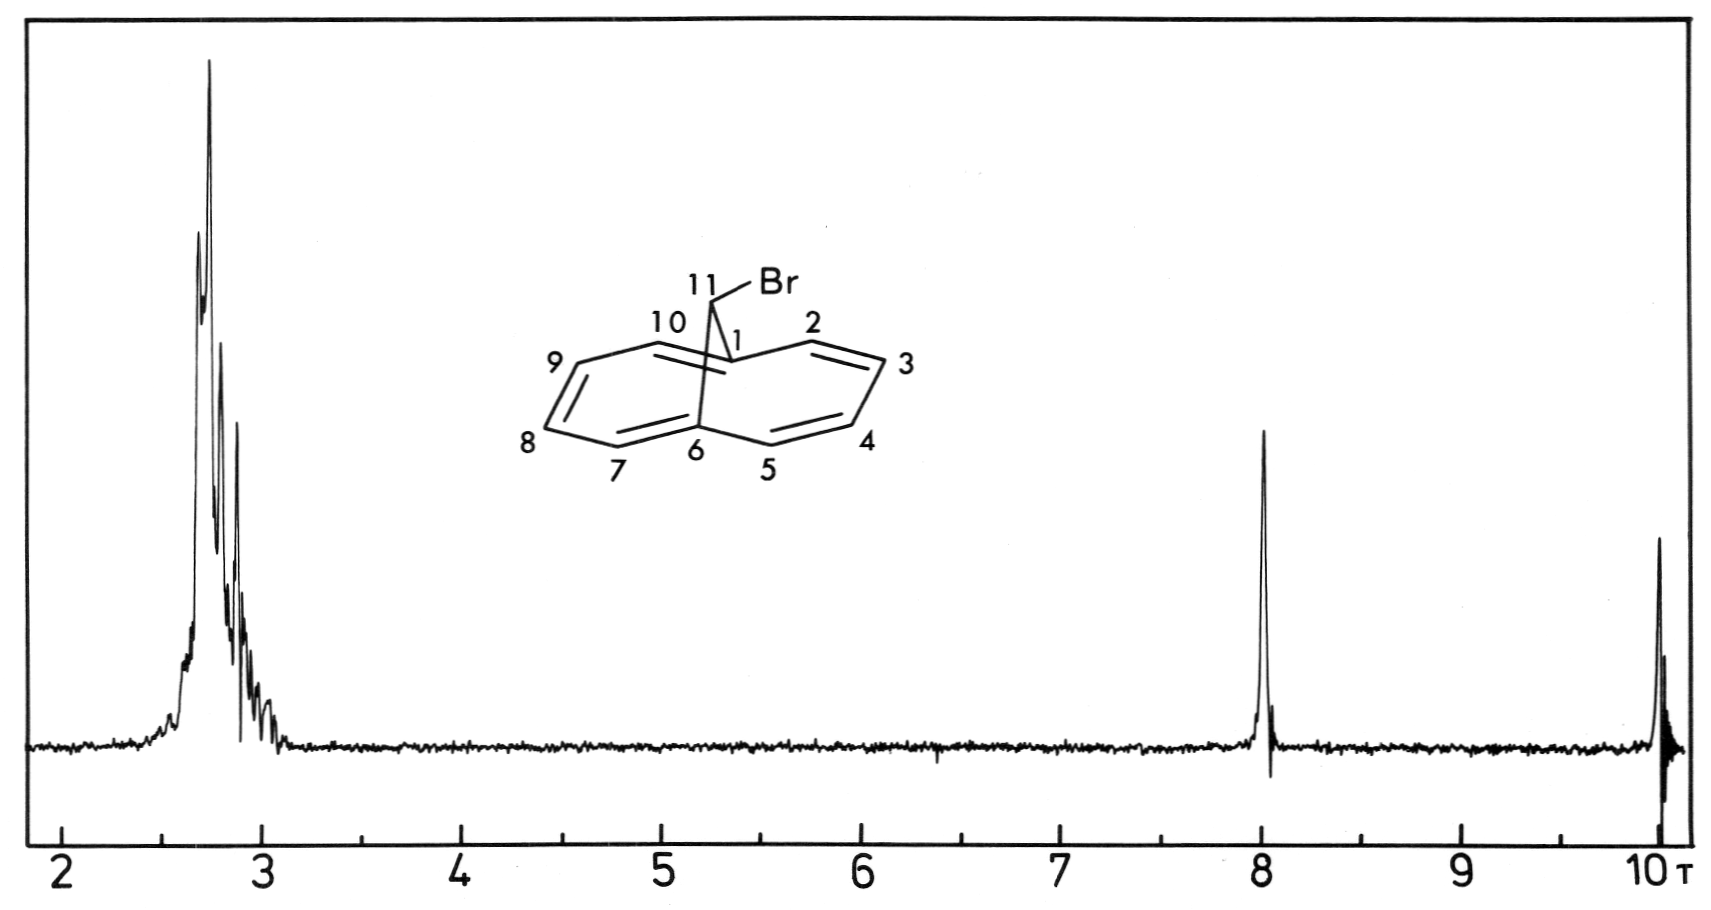
\includegraphics[width=14.48cm]{NMR_001}
\begin{alltt}
Abb. 1: \raise0.5ex\hbox{1}H-Spektrum des 11-Brom-l,6-methano-[10]annulens (25)
in CCl4 (60 MHz; TMS als innerer Standard)

 

Da eine Oxidation des Alkohols (20) nach den enttäuschenden Resul-
taten von H. Lepper \raise0.5ex\hbox{[42]} zunächst wenig aussichtsreich erschien,
wurde alternativ die Synthese des 11-Amino-1,6-methano-[10]annulens
(19) ins Auge gefasst.

Amine lassen sich im allgemeinen sehr leicht aus den um ein Kohlen-
stoffatom reicheren Carbonsäuren durch spezielle Abbaureaktionen
gewinnen \raise0.5ex\hbox{[46]}, von denen der CURTIUS-Abbau \raise0.5ex\hbox{[47]} - was Übersicht-
lichkeit des Reaktionsverlaufs und geringen apparativen Aufwand
angeht - den anderen Methoden überlegen ist. Damit zeichnet sich
folgendes Reaktionsschema ab:

\end{alltt}
\schemestart
\hspace{0.5cm}
% 11-Brom-1,6-methano-[10]annulen (25)
\chemname{
\chemfig{=_[:60]-[:12]=_[:-12]
(-[:-252]?(-[:15]Br))% 1,6 Brücke
-[:12]=_[:-12]-[:-120]=_[:-168]-[:168]?=_[:-168]-[:168]}
}{\cmpd{bromomethano10annulen}}
\arrow(.east--.west){->[\chemfig{n{-}BuLi}]}
% 11-Lithio-1,6-methano-[10]annulen (26)
\chemname{
\chemfig{=_[:60]-[:12]=_[:-12]
(-[:-252]?(-[:15]Li))% 1,6 Brücke
-[:12]=_[:-12]-[:-120]=_[:-168]-[:168]?=_[:-168]-[:168]}
}{\cmpd{lithiomethano10annulen}}
\arrow(.east--.west){->[\chemfig{CO_2}]}
% 1,6-methano-[10]annulen-11-carbonsaeure (27)
\chemname{
\chemfig{=_[:60]-[:12]=_[:-12]
(-[:-252]?(-[:15]CO_2H))% 1,6 Brücke
-[:12]=_[:-12]-[:-120]=_[:-168]-[:168]?=_[:-168]-[:168]}
}{\cmpd{methano10annulen11saeure}}
\schemestop
\\[8pt]
\schemestart
\hspace{0.75cm}
\arrow(.east--.west){->[\chemfig{SOCl_2}]}
% 1,6-methano-[10]annulen-11-carbonsaeurechlorid (28)
\chemname{
\chemfig{=_[:60]-[:12]=_[:-12]
(-[:-252]?(-[:15]COCl))% 1,6 Brücke
-[:12]=_[:-12]-[:-120]=_[:-168]-[:168]?=_[:-168]-[:168]}
}{\cmpd{chloromethano10annulen11saeure}}
\arrow(.east--.west){->[\chemfig{NaN_3}]}
% 1,6-methano-[10]annulen-11-carbonsaeureazid (29)
\chemname{
\chemfig{=_[:60]-[:12]=_[:-12]
(-[:-252]?(-[:15]CON_3))% 1,6 Brücke
-[:12]=_[:-12]-[:-120]=_[:-168]-[:168]?=_[:-168]-[:168]}
}{\cmpd{azidomethano10annulen11saeure}}
\arrow(.east--.west){->[\chemfig{{\Delta}T}]}
\schemestop
\chemnameinit{}
\begin{alltt}
\newpage
\makebox[0.8\textwidth][c]{- 9 -}


\end{alltt}
\schemestart[][west]
% 1,6-methano-[10]annulen-11-isocyanat (30)
\chemname{
% drawn counter-clockwise
\chemfig{-[:-12]=^[:12]?-[:-12]=^[:12]-[:60]=^[:168]-[:-168]
(-[:-252]?(-[:15]N{=}C{=}O))% 1,6 Brücke
=^[:168]-[:-168]=^[:-120]}
}{\cmpd{methano10annulenisocyanat}}
\arrow(aa.mid east--bb.mid west){->[\chemfig{H^{\oplus}}]}[45]
% 11-Amino-1,6-methano-[10]annulensalz
\chemname{
% drawn counter-clockwise^{\oplus}
\chemfig{-[:-12]=^[:12]?-[:-12]=^[:12]-[:60]=^[:168]-[:-168]
(-[:-252]?(-[:15]NH^{\oplus}_3))% 1,6 Brücke}
%(-[:-252]?(-[:15]\chemabove{N}{\scriptstyle\oplus}H_3))% 1,6 Brücke}
=^[:168]-[:-168]=^[:-120]}
}{Aminsalz}
\arrow(@aa.mid east--cc.mid west){->[][\chemfig{ROH}]}[-45]
% 1,6-methano-[10]annulen-11-urethan (31)
\chemname{
% drawn counter-clockwise
\chemfig{-[:-12]=^[:12]?-[:-12]=^[:12]-[:60]=^[:168]-[:-168]
(-[:-252]?(-[:15]NHCO_2R))% 1,6 Brücke
=^[:168]-[:-168]=^[:-120]}
}{\cmpd{methano10annulenurethan}}
\arrow(@bb.mid east--dd.mid west){->[\chemfig{OH^{\ominus}}]}[-45]
% 11-Amino-1,6-methano-[10]annulen 819)
\chemname{
% drawn counter-clockwise
\chemfig{-[:-12]=^[:12]?-[:-12]=^[:12]-[:60]=^[:168]-[:-168]
(-[:-252]?(-[:15]NH_2))% 1,6 Brücke
=^[:168]-[:-168]=^[:-120]}
}{\cmpd{aminomethano10annulen}}
\arrow(@cc.mid east--@dd.mid west){->[][\chemfig{H^{\oplus}}]}[45]
\schemestop
\chemnameinit{}
\begin{alltt}


Halogen-Metall-Austausch und Umsetzung des entstehenden Lithium-
Organyls (26) mit Kohlendioxid ergibt die Carbonsäure (27), die
sich über das Säurechlorid (28) und thermische Umlagerung des
Carbonsäureazids (29) in das Isocyanat (30) überführen lassen
sollte, aus dem durch alkalische oder saure Hydrolyse das Amin (19)
generiert wird.


2.1 11-Oxo-1‚6-methano-[10]annulen (15)

2.1.1 11-Amino-1,6-methano-[10]annulen (19)

2.1.1.1 1‚6-Methano-[10]annulen-11-carbonsäurechlorid (28)

Die als Ausgangsverbindung für den CURTIUS-Abbau benötigte Carbon-
säure (27) wurde bereits im Jahr 1967 von H. Lepper \raise0.5ex\hbox{[42]} in
59 \%iger Ausbeute präpariert. Durch sorgfältige Ausarbeitung der
Vorschrift konnte die Ausbeute auf 71 \% gesteigert werden, so daß
die gewünschte Verbindung (27) im 10 g - Maßstab zur Verfügung
stand.

Zur Synthese von Säurechloriden finden im allgemeinen Thionyl-
chlorid, Oxalylchlorid oder Phosphortrichlorid bei erhöhter Tem-
peratur Anwendung \raise0.5ex\hbox{[48]}. Möglichst schonende Bedingungen (niedrige
Reaktionstemperatur, kurze Reaktionszeit) erreicht man durch die
\newpage
\makebox[0.8\textwidth][c]{- 10 -}


Benutzung des Thionylchlorid-DMF- \raise0.5ex\hbox{[49]} oder Thionylchlorid-HMPT-
Komplexes \raise0.5ex\hbox{[50]}, mit denen die Carbonsäure (27) innerhalb einer
Stunde zum Säurechlorid (28) abreagiert.

\end{alltt}
\schemestart
\hspace{1.5cm}
% 1,6-methano-[10]annulen-11-carbonsaeure (27)
\chemname{
\chemfig{=_[:60]-[:12]=_[:-12]
(-[:-252]?(-[:15]CO_2H))% 1,6 Brücke
-[:12]=_[:-12]-[:-120]=_[:-168]-[:168]?=_[:-168]-[:168]}
}{\cmpd{methano10annulen11saeure}}
\arrow(.east--.west){->[\chemfig{SOCl_2}][\chemfig{DMF}]}
% 1,6-methano-[10]annulen-11-carbonsaeurechlorid (28)
\chemname{
\chemfig{=_[:60]-[:12]=_[:-12]
(-[:-252]?(-[:15]COCl))% 1,6 Brücke
-[:12]=_[:-12]-[:-120]=_[:-168]-[:168]?=_[:-168]-[:168]}
}{\cmpd{chloromethano10annulen11saeure}}
\schemestop
\chemnameinit{}

\begin{alltt}
Das 1,6-Methano-[10]annulen-11-carbonsäurechlorid (28) bildet
gelbe, hydrolyseempfindliche Nadeln vom Fp = 85 - 87\degree{}C. Die
Verbindung reagiert wie ein aliphatisches Säurechlorid: Umsetzung
mit Ammoniak bzw. Alkoholen führt zu Carbonsäureamiden bzw.
-estern.

\end{alltt}
\hspace*{-0.25cm}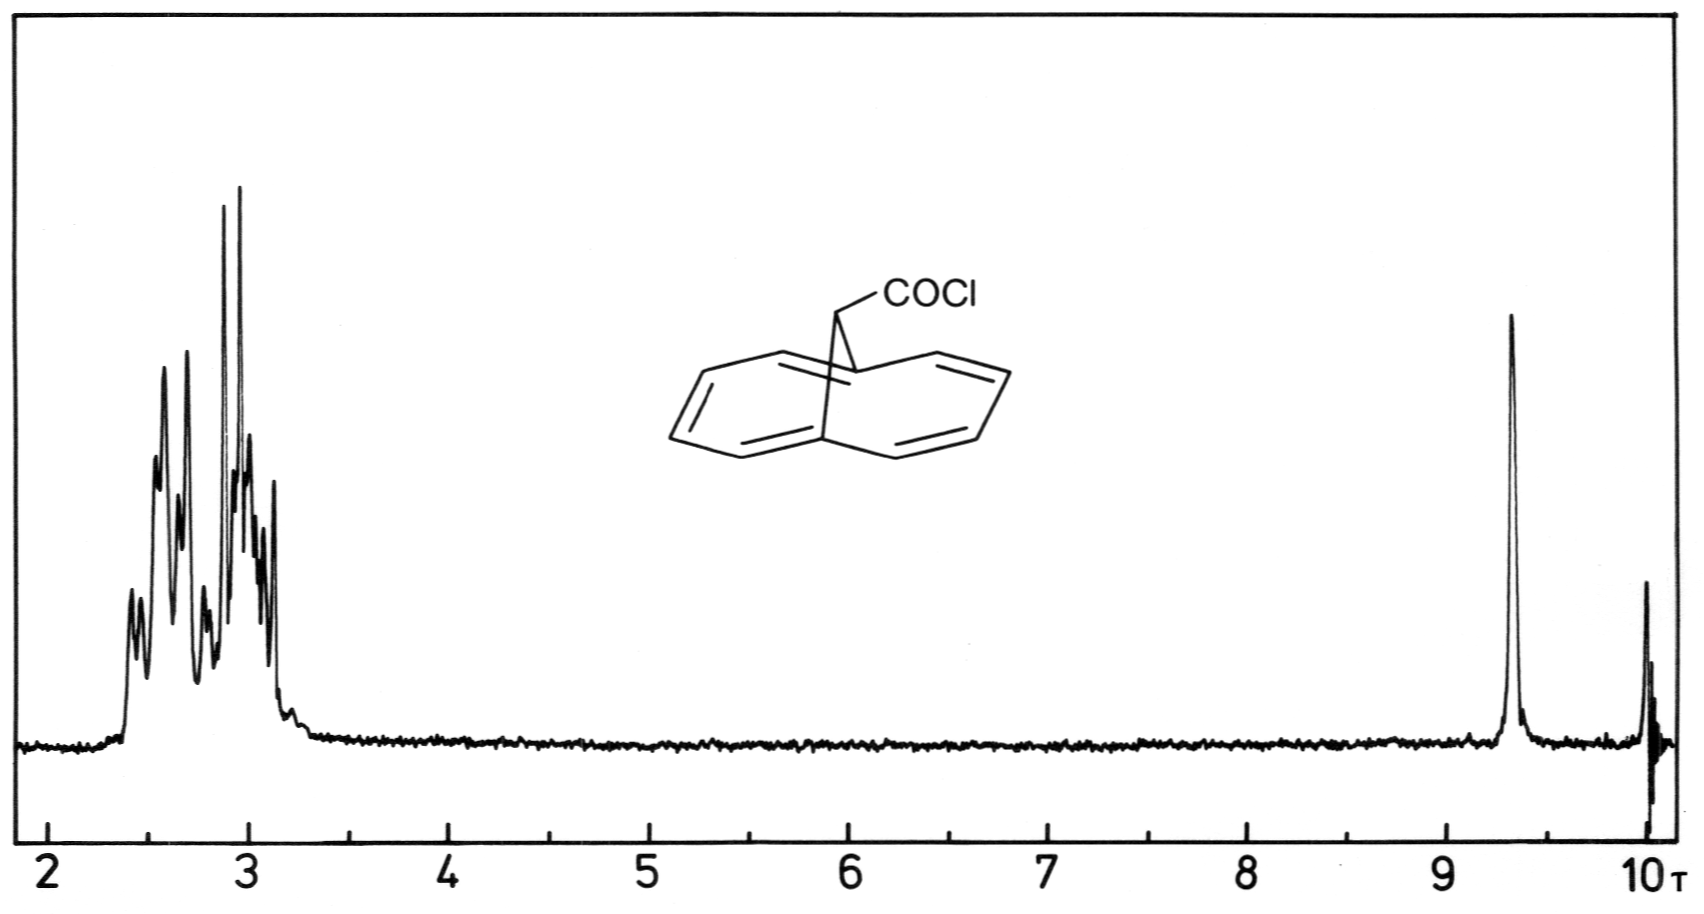
\includegraphics[width=14.427cm]{NMR_002}
\begin{alltt}
Abb. 2: \raise0.5ex\hbox{1}H-NMR-Spektrum des 1,6-Methano-[10]annulen-11-carbonsäure-
chlorids (28) in CDCl\lower0.5ex\hbox{3} (60 MHz; TMS als innerer Standard)

Das \raise0.5ex\hbox{1}H-NMR-Spektrum ist außerordentlich ähnlich dem der Säure
(27) \raise0.5ex\hbox{[42]}, einzig das Brückenproton H-11 ist um 0.5 ppm nach tie-
ferem Feld verschoben (\(\tau\) = 9.33). Das UV-Spektrum zeigt das für
1,6-Methano-[10]annulene typische Dreibandensystem.

\newpage
\makebox[0.8\textwidth][c]{- 11 -}


2.1.1.2 1‚6-Methano-[10]annulen-11-carbonsäureazid (29)

Der Austausch des Choratoms in (28) gegen die Azidgruppe gestal-
tet sich unproblematisch: In acetonischer Lösung reagiert das
Säurechlorid (28) bei 0\degree{}C fast spontan mit einer wässrigen Natrium-
azidlösung.

\end{alltt}
\schemestart
\hspace{1.5cm}
% 1,6-methano-[10]annulen-11-carbonsaeurechlorid (28)
\chemname{
\chemfig{=_[:60]-[:12]=_[:-12]
(-[:-252]?(-[:15]COCl))% 1,6 Brücke
-[:12]=_[:-12]-[:-120]=_[:-168]-[:168]?=_[:-168]-[:168]}
}{\cmpd{chloromethano10annulen11saeure}}
\arrow(.east--.west){->[\chemfig{NaN_3}][\chemfig{Aceton}]}
% 1,6-methano-[10]annulen-11-carbonsaeureazid (29)
\chemname{
\chemfig{=_[:60]-[:12]=_[:-12]
(-[:-252]?(-[:15]CON_3))% 1,6 Brücke
-[:12]=_[:-12]-[:-120]=_[:-168]-[:168]?=_[:-168]-[:168]}
}{\cmpd{azidomethano10annulen11saeure}}
\schemestop
\chemnameinit{}
\begin{alltt}

Wässrig-ätherische Aufarbeitung mit anschließender Säulenchromato-
graphie an Aluminiumoxid (Eluens: Methylenchlorid) liefert feine
gelbe Nadeln, die aus Methylenchlorid/Pentan als gelbe Quader
kristallisieren. Einen ersten Hinweis auf das Entstehen des Säure-
azids (29) gibt das Schmelzverhalten: Oberhalb von 110\degree{}C zersetzt
sich die Substanz unter starker Stickstoffentwicklung.

\end{alltt}
\hspace*{-0.25cm}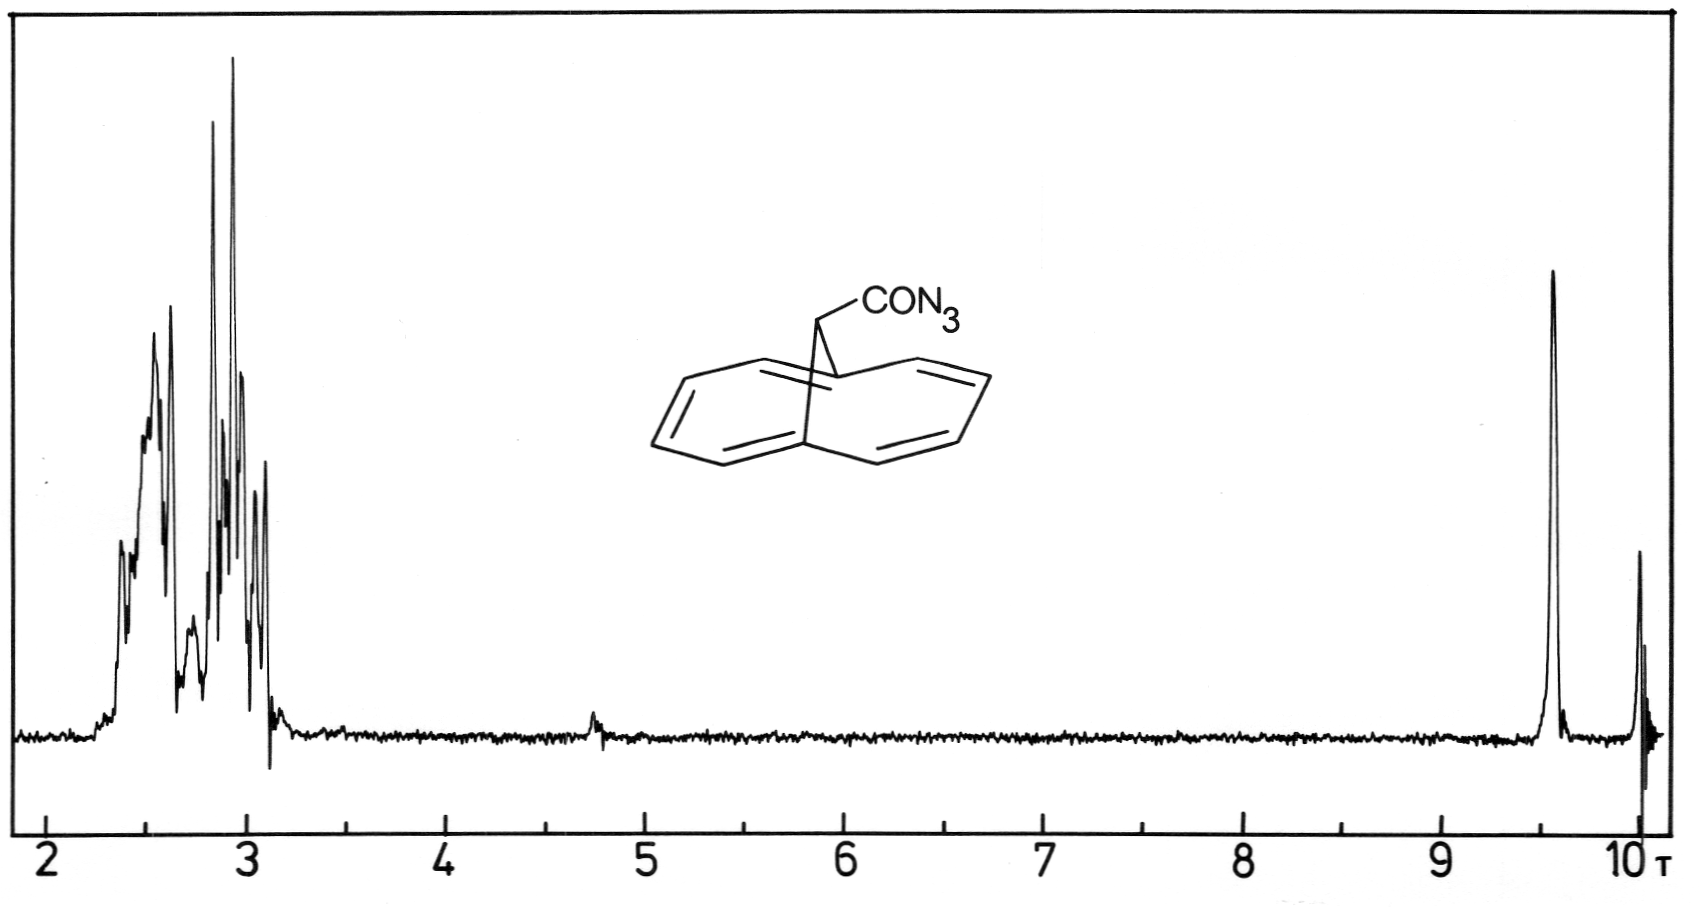
\includegraphics[width=14.385cm]{NMR_003}
\begin{alltt}
Abb. 3: \raise0.5ex\hbox{1}H-NMR-Spektrum des 1,6-Methano-[10]annulen-11-carbonsäure-
azids (29) in CD\lower0.5ex\hbox{2}Cl\lower0.5ex\hbox{2} (60 MHz; TMS als innerer Standard)

Das \raise0.5ex\hbox{1}H-NMR-Spektrum ist wenig aussagekräftig: Infolge der Pseudo-
halogeneigenschaften der Azidgruppe tritt fast keine Änderung
\newpage
\makebox[0.8\textwidth][c]{- 12 -}


gegenüber dem Säurechlorid (28) auf. Neben einem nur wenig struk-
turierten Multiplett (2 überlagerte AA'BB'-Systeme der beiden Ring-
hälften) bei \(\tau\) = 2.25 - 3.32 erscheint nur noch ein Signal für das
Brückenproton bei \(\tau\) = 9.57 - deutlich höher als im Säurechlorid
(28). Zwei Banden hoher Intensität im IR-Spektrum bei 2150 cm\raise0.5ex\hbox{-1}
(asymmetrische Streckschwingung der N=N=N - Einheit) sowie bei
1725 cm\raise0.5ex\hbox{-1} (C=O - Valenzschwingung) weisen die neue Verbindung
nachdrücklich als Carbonsäureazid aus \raise0.5ex\hbox{[51]}. Das UV-Spektrum ent-
spricht weitgehend dem des Säurechlorids (28).

2.1.1.3 4-Nitrophenyl-N-[1‚6-methano-[10]annulen-11-yl]carb-
aminat (31a)

Ersten Versuchen, das Isocyanat (30) durch thermische Einwirkung,
etwa durch Erhitzen des Carbonsäureazids (29) in inerten Lösungs-
mitteln wie Benzol oder Toluol, zu präparieren, war kein Erfolg
beschieden. Man isoliert neben wechselnden Mengen Edukt nur das
1,2-Benzocycloheptatrien-(1,4,6)-3-isocyanat (32), das vermutlich
in einer Berson-Willcott-Umlagerung \raise0.5ex\hbox{[52]} aus dem anscheinend
thermisch labilen Isocyanat (30) entsteht \raise0.5ex\hbox{[45]}.

\end{alltt}
\schemestart
\hspace{-0.5cm}
% 1,6-methano-[10]annulen-11-carbonsaeureazid (29)
\chemname{
\chemfig{=_[:60]-[:12]=_[:-12]
(-[:-252]?(-[:15]CON_3))% 1,6 Brücke
-[:12]=_[:-12]-[:-120]=_[:-168]-[:168]?=_[:-168]-[:168]}
}{\cmpd{azidomethano10annulen11saeure}}
\arrow(.mid east--.mid west){->[\chemfig{{\Delta}T}]}
% 1,6-methano-[10]annulen-11-isocyanat (30)
\chemname{
\chemleft[\chemfig{-[:-12]=^[:12]?-[:-12]=^[:12]-[:60]=^[:168]-[:-168]
(-[:-252]?(-[:15]N{=}C{=}O))% 1,6 Brücke
=^[:168]-[:-168]=^[:-120]}\chemright]
}{\cmpd{methano10annulenisocyanat}}
\arrow(.mid east--.mid west){->[\chemfig{\leadsto}]}
% Benzocycloheptatrien-isocyanat (32)
\chemname{
% drawn clockwise
\chemfig{=_[:-168]-[:168]=_[:60]-[:12]=_[:-12]%
-[:24,0.5](-[:60,0.8]N{=}C{=}O)(-[:-120,0.5])-[:24,0.5]-[:-15]=_[:-66,0.8]-[:-144]=_[:-172]-[:153]-[:60]}
}{\cmpd{benzocyclo7trienisocyanat}}
\schemestop
\chemnameinit{}
\begin{alltt}

Erhitzen des Carbonsäureazids (29) mit Alkoholen führt zwar zu den
entsprechenden Carbaminaten (31), eine alkalische Hydrolyse gemäß
dem Schema auf Seite 8 f. überstehen auch diese Verbindungen nicht.

\end{alltt}
\schemestart
% 1,6-methano-[10]annulen-11-carbonsaeureazid (29)
\chemname{
\chemfig{=_[:60]-[:12]=_[:-12]
(-[:-252]?(-[:15]CON_3))% 1,6 Brücke
-[:12]=_[:-12]-[:-120]=_[:-168]-[:168]?=_[:-168]-[:168]}
}{\cmpd{azidomethano10annulen11saeure}}
% 1,6-Methano-[10]annulen-11-urethan (31)
\arrow(.mid east--.mid west){->[\chemfig{ROH}]}
\chemname{
% drawn counter-clockwise
\chemfig{-[:-12]=^[:12]?-[:-12]=^[:12]-[:60]=^[:168]-[:-168]
(-[:-252]?(-[:15]NHCO_2R))% 1,6 Brücke
=^[:168]-[:-168]=^[:-120]}
}{\cmpd{methano10annulenurethan}}
\arrow(.mid east--.mid west){-/>}
% 11-Amino-1,6-methano-[10]annulen (19)
\chemname{
% drawn counter-clockwise
\chemfig{-[:-12]=^[:12]?-[:-12]=^[:12]-[:60]=^[:168]-[:-168]
(-[:-252]?(-[:15]NH_2))% 1,6 Brücke
=^[:168]-[:-168]=^[:-120]}
}{\cmpd{aminomethano10annulen}}
\schemestop
\chemnameinit{}
\begin{alltt}
\newpage
\makebox[0.8\textwidth][c]{- 13 -}


Nach H. R. Kricheldorf et al. \raise0.5ex\hbox{[53]} sollte man jedoch auf einem
Umweg zum Isocyanat (30) gelangen: Sie fanden, daß Carbamidsäure-
chloride, -anhydride und -ester (A) nach N-Silylierung mit
Trimethylchlorsilan/Triäthylamin oder Trimethylsilylacetamid bei
thermischer Beanspruchung in die Isocyanate (C) und eine Silizium-
verbindung (D) zerfallen.

\end{alltt}
\schemestart[0,1,line width=\bondwidth]
% Schema Kricheldorf
\chemnameinit{\chemfig{R'N-C(=[:90,0.8]O)(-[:-90]SiMe_3)-X}}
\chemname[0.75ex]{
\chemfig{R'-NH-CO-X}
}{\bf (A)}
\arrow(.mid east--.mid west){->}
\chemname[0.75ex]{
\chemfig{R'N-C(=[:90,0.8]O)(-[:-90]SiMe_3)-X}
}{\bf (B)}
\arrow(.mid east--.mid west){->[\chemfig{{\Delta}T}]}
\chemname[0.75ex]{
\chemfig{R'-N{=}C{=}O}
}{\bf (C)}
\+
\chemname[0.75ex]{
\chemfig{X-SiMe_3}
}{\bf (D)}
\schemestop
\chemnameinit{}
\\[4pt]
\schemestart
\hspace{4cm}
\chemfig{X{=\ }Cl{,\ }OR_1{,\ }O-CO-NH-R_2}
\schemestop
\begin{alltt} 

Bei den Carbaminaten R-NH-CO\lower0.5ex\hbox{2}R\lower0.5ex\hbox{1} hängt die Reaktionstemperatur bei
gleichbleibendem Rest R von R\lower0.5ex\hbox{1} ab; mit zunehmender Stabilität des
Anions R\lower0.5ex\hbox{1}O\raise0.5ex\hbox{-} nimmt sie stark ab. So wird für die 4-Nitrophenylcarb-
aminate eine Spalttemperatur von -20 - 0\degree{}C angegeben. Es lag daher
nahe, diese Sequenz auf die Synthese des Isocyanats (30) zu über-
tragen.

Tatsächlich entsteht durch dreistündiges Erhitzen des Carbonsäure-
azids (29) mit 4-Nitrophenol in Benzol laut Dünnschichtchromato-
gramm (SiO\lower0.5ex\hbox{2}/CH\lower0.5ex\hbox{2}Cl\lower0.5ex\hbox{2}) eine neue, bei 350 nm intensiv blau fluores-
zierende Substanz, die nach Säulenchromatographie an Kieselgel
(Eluens: Methylenchlorid) in Form hellgelber Nadeln vom Fp = 143 -
145\degree{}C isoliert wird. Bereits beim Versuch, die Verbindung aus
heißem Methanol umzukristallisieren, trat eine "Umesterung" ein.
Laut Dünnschichtchromatogramm entsteht neben der Ausgangsverbin-
dung (31a) ein neues Produkt, das als Methyl-N-[1,6-methano-
[10]annulen-11-yl]carbaminat (31b) identifiziert wurde.

\end{alltt}
\schemestart
% 1,6-methano-[10]annulen-11-carbonsaeureazid (29)
\chemname{
\chemfig{=_[:60]-[:12]=_[:-12]
(-[:-252]?(-[:15]CON_3))% 1,6 Brücke
-[:12]=_[:-12]-[:-120]=_[:-168]-[:168]?=_[:-168]-[:168]}
}{\cmpd{azidomethano10annulen11saeure}}
\arrow(.mid east--.mid west){->[\chemfig{R_1OH}]}
% Nitrophenyl-1,6-methano-[10]annulen-11-urethan (31a)
\chemname{
% drawn counter-clockwise
\chemfig{-[:-12]=^[:12]?-[:-12]=^[:12]-[:60]=^[:168]-[:-168]
(-[:-252]?(-[:15]NHCO_2R_1))% 1,6 Brücke
=^[:168]-[:-168]=^[:-120]}
}{\cmpd{methano10annulenurethan.a}}
\arrow(.mid east--.mid west){->[\chemfig{R_2OH}]}
% Methyl-1,6-methano-[10]annulen-11-urethan (31b)
\chemname{
% drawn counter-clockwise
\chemfig{-[:-12]=^[:12]?-[:-12]=^[:12]-[:60]=^[:168]-[:-168]
(-[:-252]?(-[:15]NHCO_2R_2))% 1,6 Brücke
=^[:168]-[:-168]=^[:-120]}
}{\cmpd{methano10annulenurethan.b}}
\schemestop
\chemnameinit{}
\\[16pt]
\schemestart
\hspace{5cm}
\chemfig[atom style={scale=0.9}]{R_1{=}-[,1.2]O-*6(-=-(-NO_2)=-=-)}
\hspace{2.4cm}
\chemfig[atom style={scale=0.9}]{R_2{=}-[,1.4]Me}
\schemestop
\begin{alltt}
\newpage
\makebox[0.8\textwidth][c]{- 14 -}


Das gebildete 4-Nitrophenyl-N-[1,6-methano-[10]annulen-11-yl]carb-
aminat (31a) scheint somit in der Tat eine sehr reaktive Spezies
darzustellen. Die Elementaranalyse macht die Summenformel
C\lower0.5ex\hbox{18}H\lower0.5ex\hbox{14}N\lower0.5ex\hbox{2}O\lower0.5ex\hbox{4} wahrscheinlich, und das \raise0.5ex\hbox{1}H-NMR-Spektrum stützt diesen
Strukturvorschlag.
           
\end{alltt}
\hspace*{-0.25cm}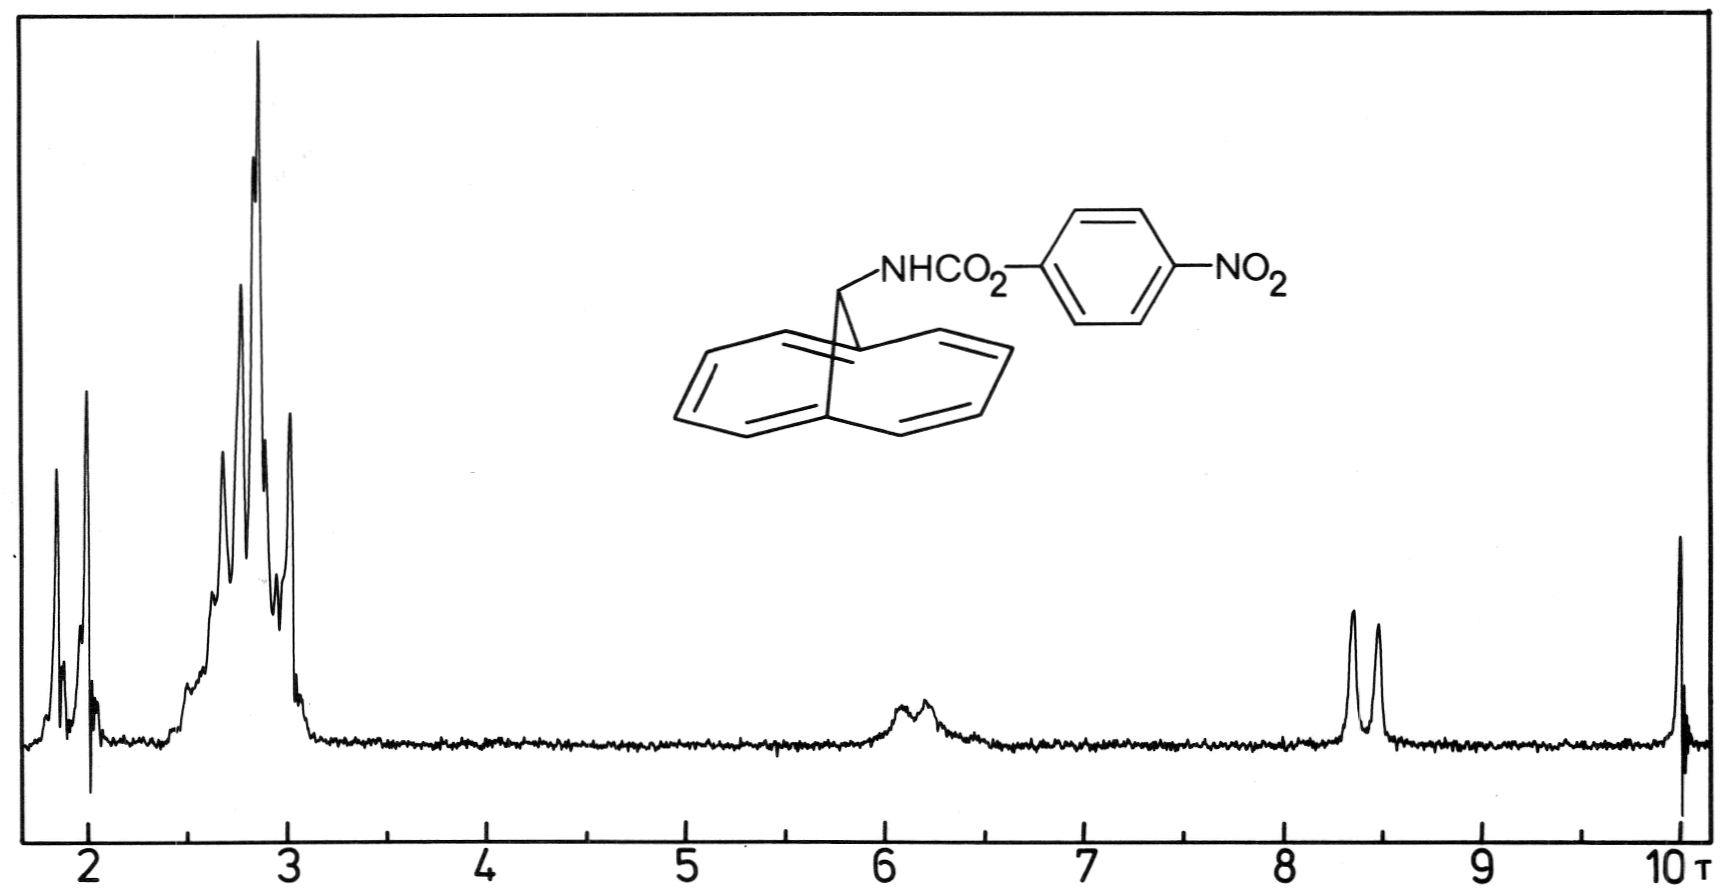
\includegraphics[width=14.68cm]{NMR_004}
\begin{alltt}
Abb. 4: \raise0.5ex\hbox{1}H-NMR-Spektrum des 4-Nitrophenyl-N-[1,6-methano-
[10]annulen-11-yl]carbaminats (31a) in CDCl\lower0.5ex\hbox{3} (60 MHz;
TMS als innerer Standard)

Bei \(\tau\) = 1.85 - 3.18 absorbieren zwölf aromatische Protonen, wobei
der A-Teil des AB-Systems für den para-substituierten Benzolring
(\(\nu\)\lower0.5ex\hbox{A} = 1.94, J\lower0.5ex\hbox{AB} = 16 Hz) deutlich vom Multiplett der übrigen
Protonen separiert ist. Die Perimeterprotonen des Annulenteils
geben Anlass zu zwei überlagerten AA'BB'-Systemen, deren Signal-
struktur starke Ähnlichkeit mit der des 11-Brom-1‚6-methano-
[10]annulens (25) (vgl. S. 8) aufweist. Brückenproton H-11 und
Amidproton (Dubletts zentriert bei \(\tau\) = 8.43 bzw. \(\tau\) = 6.16) bilden
ein weiteres AB-System mit J\lower0.5ex\hbox{AB} = 13 Hz. Auch das Amidproton
(normale Absorptionslage: 4.0 - 5.0 \(\tau\)) unterliegt noch dem Ring-
stromeffekt, wenn auch nicht mehr in dem Maße wie das Brücken-
proton (normale Lage: 5.9 \(\tau\) \raise0.5ex\hbox{[54]}) für eine höhere Position des
Amidprotons über dem 10\(\pi\)-Elektronensystem spricht.
\newpage
\makebox[0.8\textwidth][c]{- 15 -}


Das UV-Spektrum zeigt neben einem Hauptmaximum bei 256 nm (\(\epsilon\) =
58700) nicht mehr die für [10]Annulene typische Feinaufspaltung
im länger welligen Bereich, sondern nur noch drei Schultern bei
295 (13400), 387 (282) und 397 nm (188).

2.1.1.4 1‚6-Methano-[10]annulen-11-isocyanat (30)

Im weiteren Verlauf der Synthese wird eine Lösung des Carbaminats
(31a) in Methylenchlorid bei 0\degree{}C zunächst mit Triäthylamin als
Protonenakzeptor und dann mit Trimethylchlorsilan versetzt. Nach
etwa fünf Stunden hat sich fast alles Edukt umgesetzt.

\end{alltt}
\schemestart
\hspace{-0.5cm}
% Nitrophenyl-1,6-methano-[10]annulen-11-urethan (31)
\chemname{
% drawn counter-clockwise
\chemfig{-[:-12]=^[:12]?-[:-12]=^[:12]-[:60]=^[:168]-[:-168]
(-[:-252]?(-[:15]NHCO_2R_1))% 1,6 Brücke
=^[:168]-[:-168]=^[:-120]}
}{\cmpd{methano10annulenurethan}}
\arrow(.mid east--.mid west){->}
% N-Trimethylsilyl-1,6-methano-[10]annulen-11-urethan
\chemfig{
% drawn counter-clockwise
-[:-12]=^[:12]?-[:-12]=^[:12]-[:60]=^[:168]-[:-168]
(-[:-252]?(-[:15]N(-[:135,0.9]Me_3Si)(-[,0.8]C(=[:45,0.9]O)(-[:-45]OR_1))))% 1,6 Brücke
=^[:168]-[:-168]=^[:-120]}
\arrow(.mid east--.mid west){->}
% 1,6-methano-[10]annulen-11-isocyanat (30)
\chemname{
% drawn counter-clockwise
\chemfig{-[:-12]=^[:12]?-[:-12]=^[:12]-[:60]=^[:168]-[:-168]
(-[:-252]?(-[:15]N{=}C{=}O))% 1,6 Brücke
=^[:168]-[:-168]=^[:-120]}
}{\cmpd{methano10annulenisocyanat}}
\schemestop
\begin{alltt}

Durch Säulenchromatographie an Kieselgel (Eluens: Methylenchlorid)
gelangt man in 71 \%iger Ausbeute zum 1,6-Methano-[10]annulen-11-
isocyanat (30), das aus Äther/Pentan in Form hellgelber, recht-
eckiger Pinakoide vom Fp = 64 - 65\degree{}C kristallisiert.


\end{alltt}
\hspace*{-0.25cm}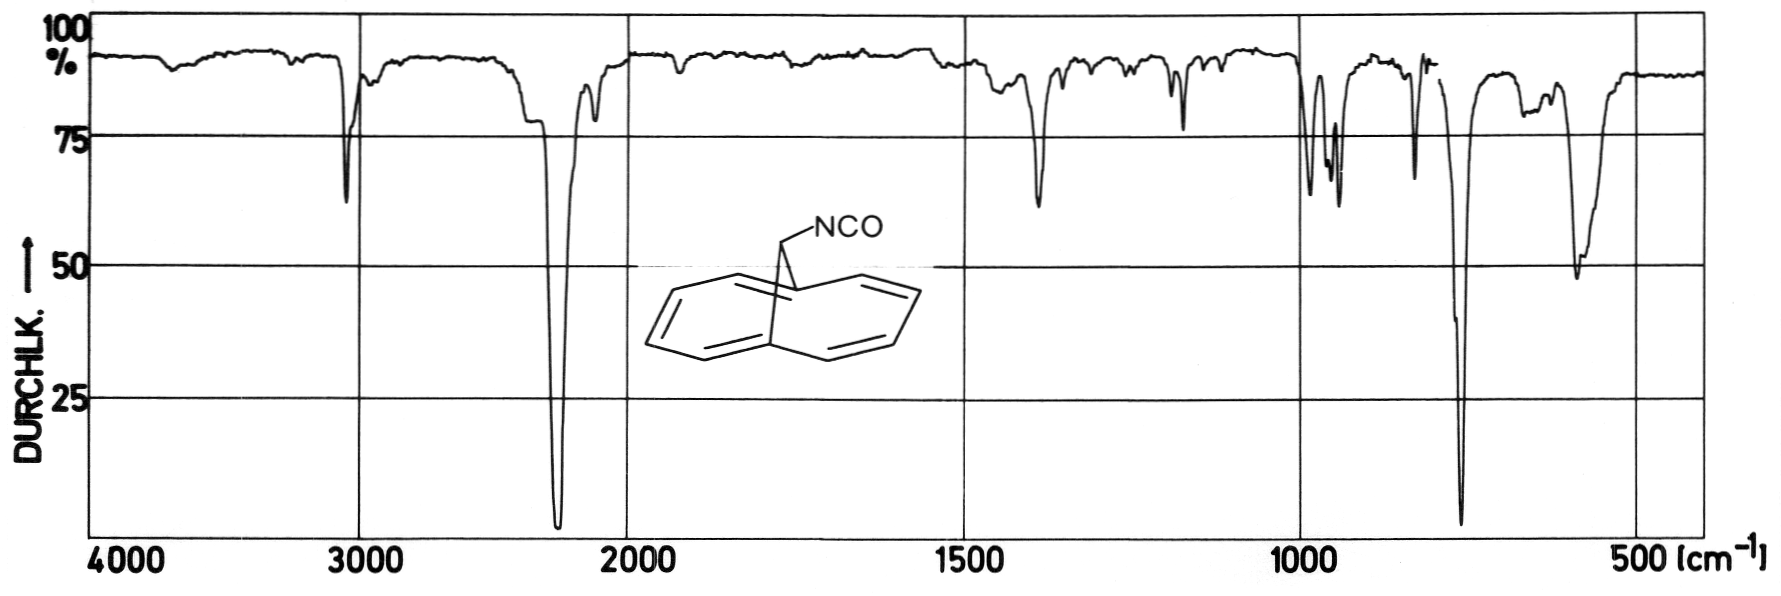
\includegraphics[width=14.68cm]{IR_005}
\begin{alltt}
Abb. 5: IR-Spektrum des 1‚6-Methano-[10]annulen-11-isocyanats (30)
(4000 - 820 cm\raise0.5ex\hbox{-1} in CCl\lower0.5ex\hbox{4}, 820 - 500 cm\raise0.5ex\hbox{-1} in CS\lower0.5ex\hbox{2})



Das IR-Spektrum wird beherrscht von der starken Bande bei 2258 cm\raise0.5ex\hbox{-1},
die die asymmetrische Streckschwingung der Isocyanat-Gruppe reprä-
\newpage
\makebox[0.8\textwidth][c]{- 16 -}


sentiert. Bei einer kleineren Bande bei 594 cm\raise0.5ex\hbox{-1} handelt es sich
um die "Bending"-Schwingung der funktionellen Gruppe. Auch der
[10]Annulenteil lässt sich im IR-Spektrum identifizieren: Die
charakteristischen C-H - Valenzschwingungen bei 3042 cm\raise0.5ex\hbox{-1} (Peri-
meterprotonen) und 2950 cm\raise0.5ex\hbox{-1} (Brücke) sowie die "Out-of-Plane"-
Schwingung bei 766 cm\raise0.5ex\hbox{-1} sprechen für die angenommene Struktur.

\end{alltt}
\hspace*{-0.25cm}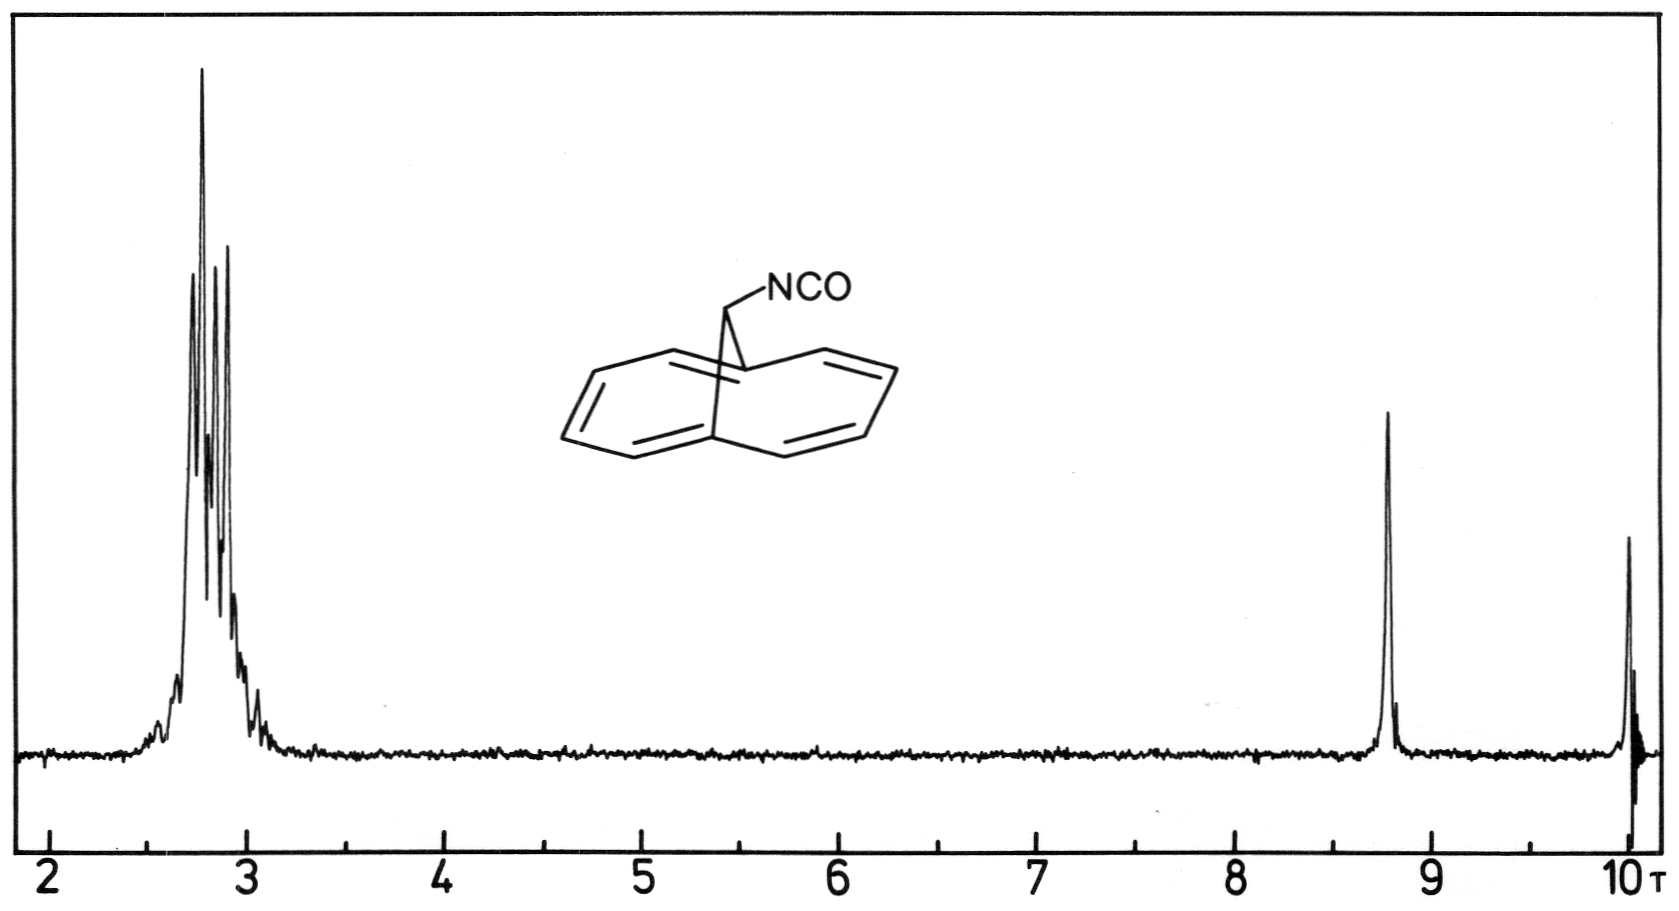
\includegraphics[width=14.216cm]{NMR_006}
\begin{alltt}
Abb. 6: \raise0.5ex\hbox{1}H-NMR-Spektrum des 1,6-Methano-[10]annulen-11-isocyanats
(30) in CCl\lower0.5ex\hbox{4} (60 MHz; TMS als innerer Standard)

Das \raise0.5ex\hbox{1}H-NMR-Spektrum zeigt die für ein brückensubstituiertes
[10]Annulen typischen Absorptionen: Ein Multiplett bei \(\tau\) = 2.45 -
3.22 für die aromatischen Protonen und ein Singulett bei \(\tau\) = 8.79
für das Wasserstoffatom H-11 sind die einzigen Signale des
Spektrums.

Für eine Verseifung des Isocyanats (30) scheiden die sonst
üblichen Hydrolysemethoden - starke Mineralsäuren bei erhöhter
Temperatur \raise0.5ex\hbox{[55]} - aus, da das [10]Annulensystem leicht Umlagerun-
gen vom Berson-Willcott-Typ \raise0.5ex\hbox{[52]} eingeht, besonders wenn durch
entsprechende Substituenten an C-11 die Aktivierungsenergie der
Umlagerung drastisch herabgesetzt ist \raise0.5ex\hbox{[56]}. In einem ersten Ver-
such wurde daher in Anlehnung an eine Vorschrift von W. Schröck \raise0.5ex\hbox{[57]}
eine ätherische Lösung des Isocyanats (30) bei 0\degree{}C mit verdünnter
\newpage
\makebox[0.8\textwidth][c]{- 17 -}


Natronlauge unterschichtet, wobei sich das Natriumsalz der
N-[1,6-Methano-[10]annulen-11-yl]carbaminsäure bildet. Nach zwei-
stündigem Rühren wird vorsichtig mit der äquivalenten Menge 2n -
Schwefelsäure neutralisiert. Dabei sollte unter Decarboxylierung
der Carbaminsäure das Amin (19) entstehen. Es lässt sich auch ein
gelbes Öl isolieren, das jedoch laut \raise0.5ex\hbox{1}H-NMR-Spektrum nur aus den
Folgeprodukten einer Umlagerung des 11-Amino-1,6-methano-
[10]annulens (19) besteht.

\end{alltt}
\schemestart
\hspace{-0.5cm}
\chemnameinit{\chemfig{=_[:-168]-[:168]=_[:60]-[:12]=_[:-12]%
-[:24](-[:60]NH_2)-[:-15]=_[:-66,0.8]-[:-144]=_[:-172]-[:153]-[:60]}
}
% 1,6-methano-[10]annulen-11-isocyanat (30)
\chemname{
\chemfig{-[:-12]=^[:12]?-[:-12]=^[:12]-[:60]=^[:168]-[:-168]
(-[:-252]?(-[:15]N{=}C{=}O))% 1,6 Brücke
=^[:168]-[:-168]=^[:-120]}
}{\cmpd{methano10annulenisocyanat}}
\arrow(.mid east--.mid west){->[\chemfig{OH^{\ominus}}]}
% 1,6-methano-[10]annulen-11-carbaminat (33)
\chemname{
\chemfig{-[:-12]=^[:12]?-[:-12]=^[:12]-[:60]=^[:168]-[:-168]
(-[:-252]?(-[:15]NHCO^{\ominus}_2))% 1,6 Brücke
=^[:168]-[:-168]=^[:-120]}
}{\cmpd{methano10annulencarbaminat}}
\arrow(.mid east--.mid west){->[\chemfig{H^{\oplus}}]}
% Benzocycloheptatrien-amin (34)
\chemname{
% drawn clockwise
\chemfig{=_[:-168]-[:168]=_[:60]-[:12]=_[:-12]%
-[:24,0.5](-[:60,0.8]NH_2)(-[:-120,0.5])-[:24,0.5]-[:-15]=_[:-66,0.8]-[:-144]=_[:-172]-[:153]-[:60]}
}{\cmpd{benzocyclo7trienamin}}
\schemestop
\chemnameinit{}
\begin{alltt}

Bei der gesuchten Verbindung (19] handelt es sich wahrscheinlich
um eine relativ empfindliche Spezies, die unter Oxidationsbedin-
gungen ebenfalls nicht zum gewünschten Keton (15) abreagieren
dürfte. Auf dieser Stufe der Synthese wurden daraufhin weitere
Versuche zurückgestellt. Eine erneute Aufnahme der Experimente
war nur für den Fall geplant, daß auch die Oxidation des 11-Hydroxy-
1,6-methano-[10]annulens (20) nicht zum 11-Oxo-1,6-methano-
[10]annulen (15) führen würde.

Die letzten Versuche auf diesem Gebiet datieren von 1967 \raise0.5ex\hbox{[42]}. Seit
diesem Zeitpunkt sind jedoch die Oxidationsmethoden laufend ver-
bessert worden. Besonders durch die Einführung von Dimethylsulf-
oxid \raise0.5ex\hbox{[58]} als Oxidationsmittel konnte eine Vielzahl von bis dahin
noch nicht bekannten Ketonen bzw. Aldehyden dargestellt werden.
\newpage
\makebox[0.8\textwidth][c]{- 18 -}


2.1.2 11-Hydroxy-1,6-methano-[1ÜJannulen (20)

Ausgehend vom 11-Brom-1,6-methano-[1O]annulen (25) ist das
11-Hydroxy-1,6-methano-[10]annulen (20) in einer durch Arbeiten
von H. Lepper \raise0.5ex\hbox{[42]} vorgezeichneten, dreistufigen Reaktionsfolge
darstellbar.

\end{alltt}
\schemestart
\hspace{-0.5cm}
% 11-Brom-1,6-methano-[10]annulen (25)
\chemname{
\chemfig{=_[:60]-[:12]=_[:-12]
(-[:-252]?(-[:15]Br))% 1,6 Brücke
-[:12]=_[:-12]-[:-120]=_[:-168]-[:168]?=_[:-168]-[:168]}
}{\cmpd{bromomethano10annulen}}
\arrow(.mid east--.mid west)
% 11-Acetoxy-1,6-methano-[10]annulen (35)
\chemname{
\chemfig{=_[:60]-[:12]=_[:-12]
(-[:-252]?(-[:15]OCOCH_3))% 1,6 Brücke
-[:12]=_[:-12]-[:-120]=_[:-168]-[:168]?=_[:-168]-[:168]}
}{\cmpd{acetoxymethano10annulen}}
\arrow(.mid east--.mid west)
% 11-Hydroxy-1,6-methano-[10]annulen (20)
\chemname{
\chemfig{=_[:60]-[:12]=_[:-12]
(-[:-252]?(-[:15]OH))% 1,6 Brücke
-[:12]=_[:-12]-[:-120]=_[:-168]-[:168]?=_[:-168]-[:168]}
}{\cmpd{hydoxymethano10annulen}}
\schemestop
\chemnameinit{}
\begin{alltt}

Wegen der nur geringen Reaktivität des Bromids (25) kann der
Alkohol (20) nicht durch direkte Hydrolyse mit Basen syntheti-
siert werden. Bei Umsetzung des Bromids (25) mit Silberacetat in
Eisessig erhält man jedoch in 60 \%iger Ausbeute das 11-Acetoxy-
1,6-methano-[10]annulen (35). Die Reaktionsträgheit des Bromids
(25) dürfte wohl auf die Tatsache zurückzuführen sein, daß die
Brücke mit dem Substituenten in die 10 \(\pi\)-Elektronenwolke oberhalb
des Perimeters eingebettet ist \raise0.5ex\hbox{[13b]}, wodurch die Annäherung
eines Reaktionspartners erheblich behindert wird. Bei der Spaltung
des Acetates (35) zum Alkohol (20) ergeben sich weitere Schwierig-
keiten: Konventionelle Methoden wie alkalische Verseifung, basen-
katalysierte Umesterung in Methanol und Umsetzung mit Lithium-
aluminiumhydrid sowie Methyllithium ergeben nur Umlagerungspro-
dukte des 11-Hydroxy-1,6-methano-[10]annulens (20). Wegen der
engen elektronischen Verwandtschaft der Hydroxylgruppe mit der
Amingruppierung sind angesichts dieser Befunde die negativen
Resultate bei der Hydrolyse des Isocyanats (30) verständlich. Erst
eine Behandlung des Acetates (35) mit Methylmagnesiumjodid und
anschließende Aufarbeitung mit gesättigter Ammoniumchloridlösung,
deren Acidität gerade zur Hydrolyse der Reaktionsmischung - aber
nicht mehr zur Umlagerung - ausreicht, führt zum Erfolg.

\newpage
\makebox[0.8\textwidth][c]{- 19 -}


2.1.2.1 11-Acetoxy-1‚6-methano-[10]annulen (35)

Bei kritischer Nacharbeitung der angegebenen Synthesefolge kann
die Ausbeute des Schrittes Bromid (25) \(\longrightarrow\) Acetat (35) auf
71 - 78 \% d.Th. gesteigert werden.

\end{alltt}
\schemestart
\hspace{1.5cm}
% 11-Brom-1,6-methano-[10]annulen (25)
\chemname{
\chemfig{=_[:60]-[:12]=_[:-12]
(-[:-252]?(-[:15]Br))% 1,6 Brücke
-[:12]=_[:-12]-[:-120]=_[:-168]-[:168]?=_[:-168]-[:168]}
}{\cmpd{bromomethano10annulen}}
\arrow(.mid east--.mid west){->[\chemfig{AgOAc}]}
% 11-Acetoxy-1,6-methano-[10]annulen (35)
\chemname{
\chemfig{=_[:60]-[:12]=_[:-12]
(-[:-252]?(-[:15]OCOCH_3))% 1,6 Brücke
-[:12]=_[:-12]-[:-120]=_[:-168]-[:168]?=_[:-168]-[:168]}
}{\cmpd{acetoxymethano10annulen}}
\schemestop
\chemnameinit{}
\begin{alltt}

Das Acetat (35) kristallisiert aus Petroläther (40-60) in Form
gelber Nadeln vom Fp = 92 - 93\degree{}C.

\end{alltt}
\hspace*{-0.25cm}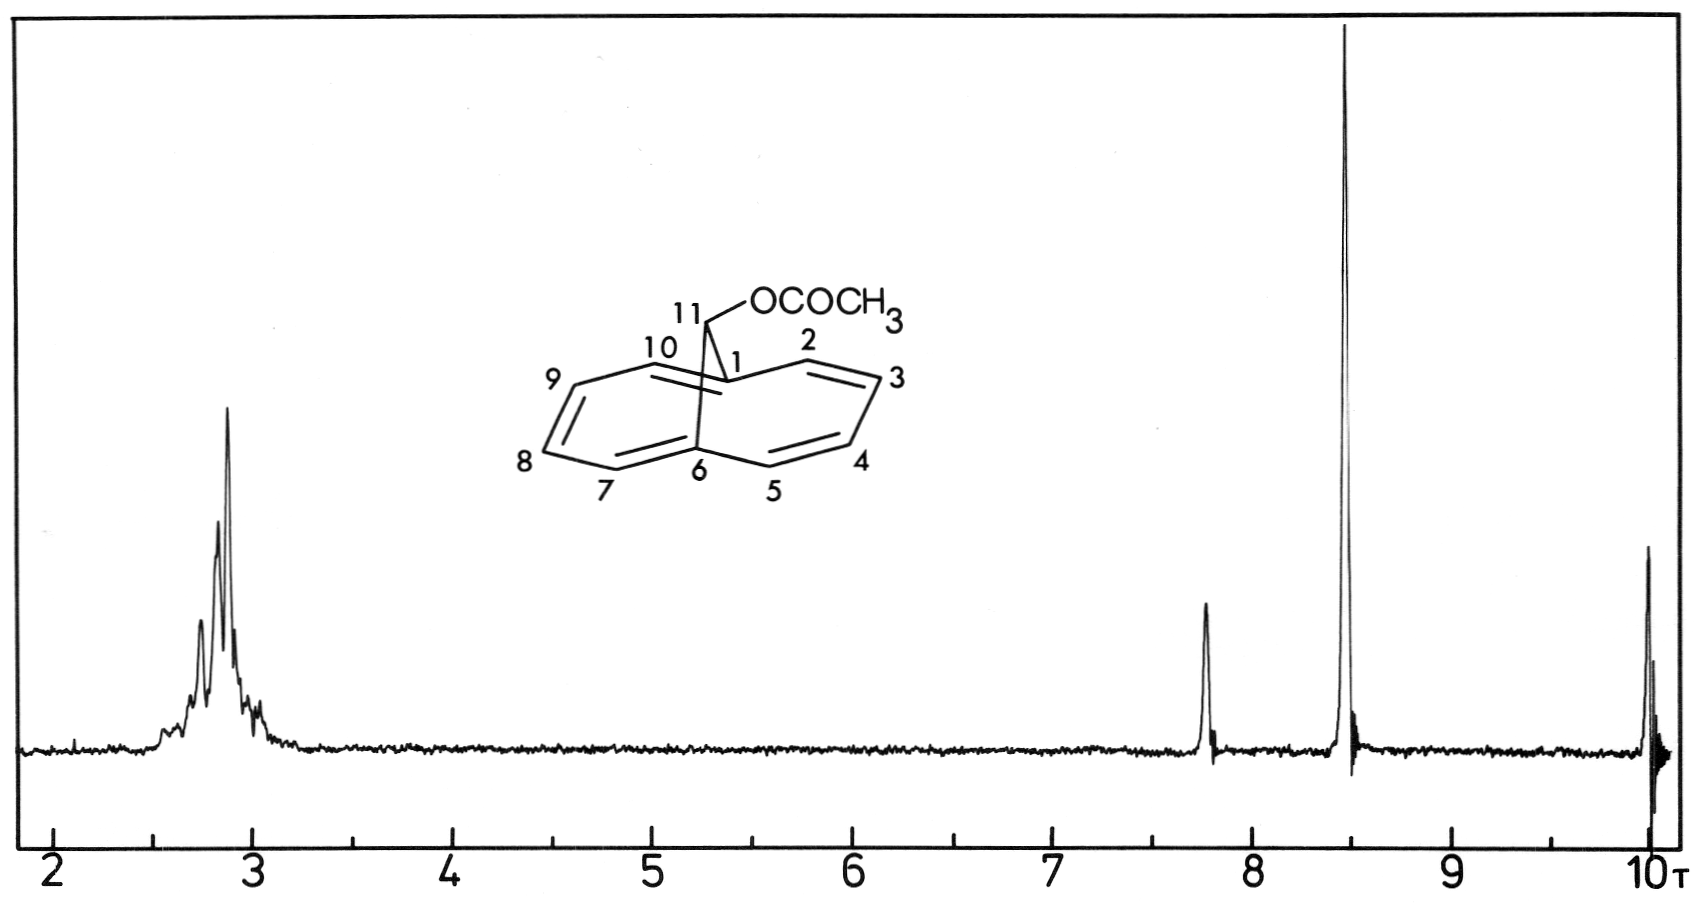
\includegraphics[width=14.351cm]{NMR_007}
\begin{alltt}
Abb. 7: \raise0.5ex\hbox{1}H-NMR-Spektrum des 11-Acetoxy-1,6-methano-[1O]annulen
(35) in CCl\lower0.5ex\hbox{4} (60 MHz; TMS als innerer Standard)

Im \raise0.5ex\hbox{1}H-NMR-Spektrum findet sich ein enges Multiplett bei \(\tau\) = 2.63 -
3.28 für die Annulenprotonen H-1 - H-10 sowie je ein Singulett
für das Brückenproton bei \(\tau\) = 7.87 und die Methylgruppe des Acetat-
restes bei \(\tau\) = 8.55 .

\newpage
\makebox[0.8\textwidth][c]{- 20 -}


2.1.2.2 11-Hydroxy-1,6-methano-[10]annulen (20)

Die Präparierung des Alkohols (2D) im Gramm-Maßstab gestaltete
sich wider Erwarten problematisch, da sich die Reaktionsvor-
schrift \raise0.5ex\hbox{[42]} als nicht reproduzierbar erwies.

\end{alltt}
\schemestart
\hspace{1.5cm}
% 11-Acetoxy-1,6-methano-[10]annulen (35)
\chemname{
\chemfig{=_[:60]-[:12]=_[:-12]
(-[:-252]?(-[:15]OCOCH_3))% 1,6 Brücke
-[:12]=_[:-12]-[:-120]=_[:-168]-[:168]?=_[:-168]-[:168]}
}{\cmpd{acetoxymethano10annulen}}
\arrow(.mid east--.mid west){->[\chemfig{MeMgJ}]}
% 11-Hydroxy-1,6-methano-[10]annulen (20)
\chemname{
\chemfig{=_[:60]-[:12]=_[:-12]
(-[:-252]?(-[:15]OH))% 1,6 Brücke
-[:12]=_[:-12]-[:-120]=_[:-168]-[:168]?=_[:-168]-[:168]}
}{\cmpd{hydoxymethano10annulen}}
\schemestop
\chemnameinit{}
\begin{alltt}

Gibt man jedoch nach einer Modifikation von V. Hautenstrauch \raise0.5ex\hbox{[59]}
das Acetat [35) nicht in Lösung \leavevmode\raise0.5ex\hbox{*}) sondern in fester Form zu der
ätherischen GRIGNARD-Verbindung, so isoliert man die gesuchte Ver-
bindung (20) in über 70 \%iger Ausbeute als gelbe monokline Prismen

 
\end{alltt}
\hspace*{-0.25cm}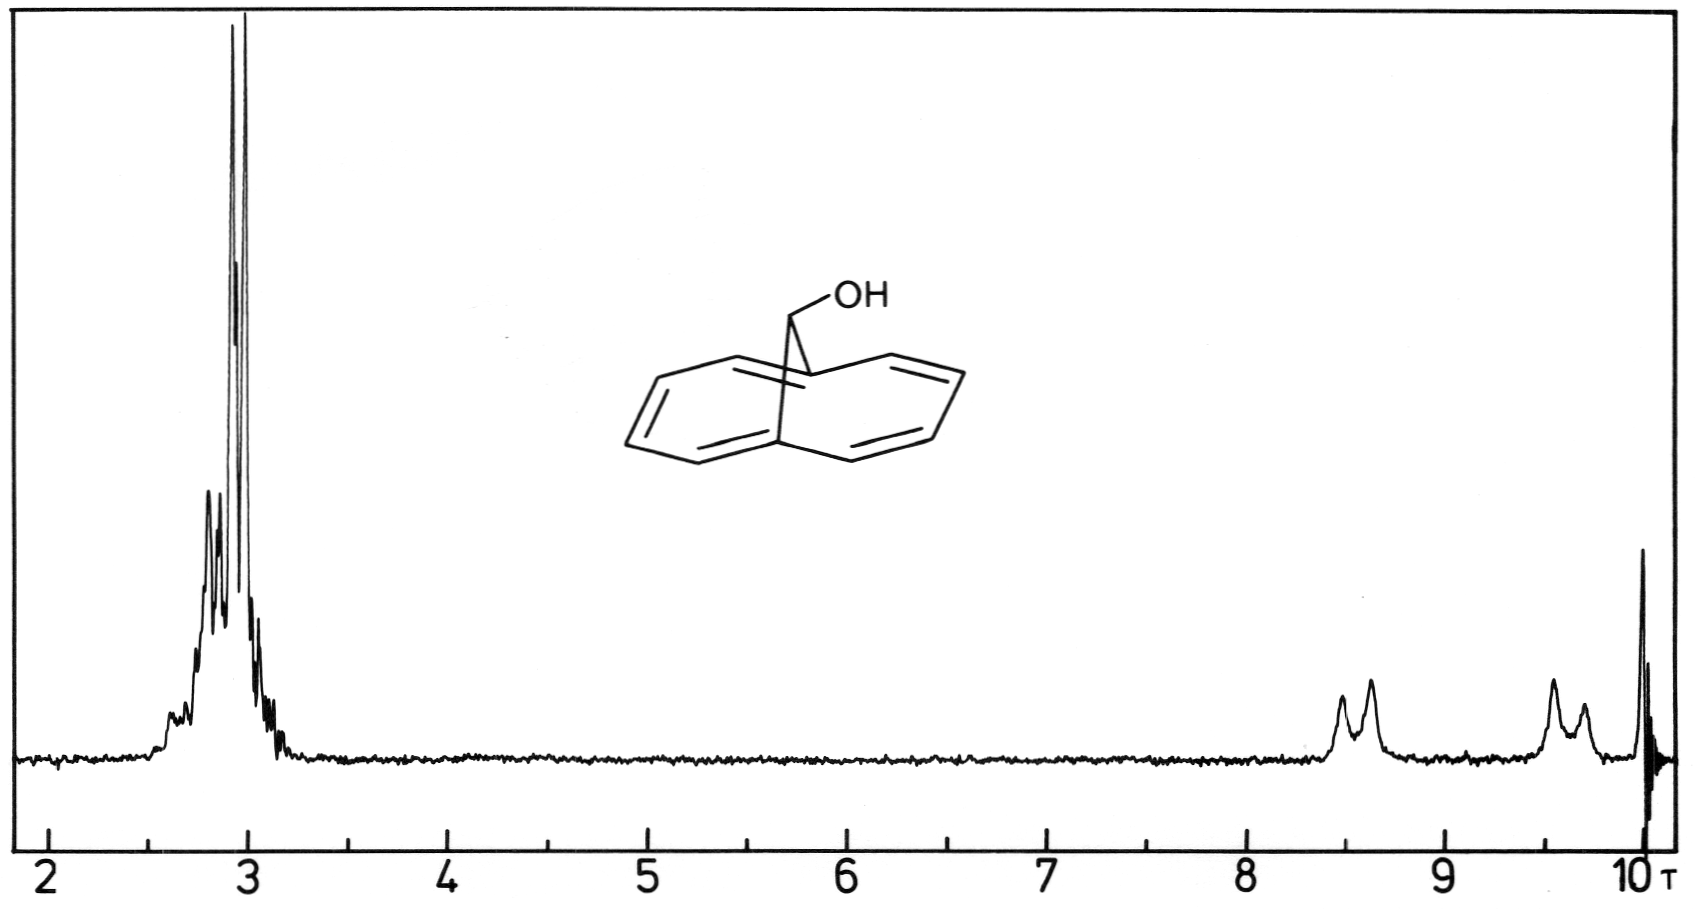
\includegraphics[width=14.351cm]{NMR_008}
\begin{alltt}
Abb. 8: \raise0.5ex\hbox{1}H-NMR-Spektrum des 11-Hydroxy-1,6-methano-[10]annulens
(20) in CDCl\lower0.5ex\hbox{3} (60 MHz; TMS als innerer Standard)

\(\overline{\hspace{7cm}}\)
\leavevmode\raise0.5ex\hbox{*}) Das als Lösungsmittel verwendete THF ist in jedem Verhältnis
   mit Wasser mischbar und dürfte daher für einen erhöhten Phasen-
   transfer von Protonen zwischen wässriger und ätherischer Schicht
   bei der Aufarbeitung verantwortlich sein, wodurch anscheinend
   unkontrollierte Umlagerungen des Alkohols (20) induziert wer-
   den.

\newpage
\makebox[0.8\textwidth][c]{- 21 -}


mit dem Schmelzpunkt 70 - 71\degree{}C. Ausgehend vom Naphthalin wird das
11-Hydroxy-1,6-methano-[10]annulen (20) in einer Gesamtausbeute
von 2.5 - 6.0 \% d.Th. zugänglich.

Neben dem für die Annulenprotonen charakteristischen Multiplett
bei \(\tau\) = 2.37 - 3.04 erscheint im \raise0.5ex\hbox{1}H-NMR-Spektrum ein AB-System
für Alkohol- und Brückenproton bei \(\nu\)\lower0.5ex\hbox{A} = 8.41 \(\tau\) und \(\nu\)\lower0.5ex\hbox{B} = 9.46 \(\tau\)
(J\lower0.5ex\hbox{AB} = 9.3 Hz). Eine Spin-Spin-Kopplung des Systems CH-OH wird
nur dann beobachtet, wenn kein schneller intermolekularer Aus-
tausch der Hydroxyprotonen über Wasserstoffbrücken erfolgt \raise0.5ex\hbox{[60]}.
Die breite Signalstruktur spricht dafür, daß der Austausch bei
diesem Molekül temperaturabhängig ist. Die Temperatur im \raise0.5ex\hbox{1}H-NMR-
Spektrometer scheint bereits ziemlich nahe am Koaleszenzpunkt zu
liegen, so daß anzunehmen ist, daß bei einer Erhöhung der Tempe-
ratur nur noch je ein Singulett für Brücken- bzw. Alkoholproton
beobachtbar wird. Bei Zugabe von Essigsäure ändert sich das Spek-
trum in charakteristischer Weise, da freie Protonen die Austausch-
reaktion katalysieren: Das Brückenproton absorbiert jetzt als
Singulett bei \(\tau\) = 8.55, während das Alkoholproton unter dem Signal
für das Säureproton verborgen ist.

2.1.2.3 Oxidation des 11-Hydroxy-1,6-methano-[10]annulens (20)

Für die Oxidation aliphatischer Alkohole steht in der organischen
Chemie ein breites Spektrum an Reagentien zur Auswahl \raise0.5ex\hbox{[40]}.
Erwähnung an dieser Stelle verdienen besonders Chrom-(VI)-oxid in
Schwefelsäure (JONES-Reagens \raise0.5ex\hbox{[61]}) oder Pyridin \raise0.5ex\hbox{[62]}, Mangan-
(IV)-oxid \raise0.5ex\hbox{[63]}, Aluminium(III)isopropanolat in Aceton (OPPENHAUER-
Dxidation \raise0.5ex\hbox{[64]} sowie Blei(IV]acetat in Pyridin \raise0.5ex\hbox{[65]}.

Um möglichst schonende Bedingungen einzuhalten, wurden aus der
Fülle der Methoden nur solche ausgewählt, deren Reaktionstempe-
ratur in einem Bereich von 0 - 20\degree{}C liegt. Exemplarisch für die
angegebenen Oxidationsmittel wurden Dipyridin-chrom(VI)oxid in
Methylenchlorid \raise0.5ex\hbox{[66]}, aktives Mangan(IV)oxid in Aceton \raise0.5ex\hbox{[63b]} und

\newpage
\makebox[0.8\textwidth][c]{- 22 -}


Blei(IV)acetat in Pyridin \raise0.5ex\hbox{[65]} eingesetzt. Bei jeder dieser Umset-
zungen mit dem Alkohol (20) bestanden die Reaktionsprodukte zu
über 90 \% aus Naphthalin (21). In wechselnden Mengen konnten da-
neben noch andere Substanzen nachgewiesen werden, bei denen es
sich jedoch in keinem Fall um das gesuchte Keton (15) handelte.
Eine Verbindung konnte \raise0.5ex\hbox{1}H-NMR-spektroskopisch als 1-Naphthaldehyd
(36) identifiziert werden \raise0.5ex\hbox{[42b]}.
\end{alltt}
\schemestart
\hspace{-0.5cm}
% 11-Hydroxy-1,6-methano-[10]annulen (20)
\chemname[2.0ex]{
\chemfig{=_[:60]-[:12]=_[:-12]
(-[:-252]?(-[:15]OH))% 1,6 Brücke
-[:12]=_[:-12]-[:-120]=_[:-168]-[:168]?=_[:-168]-[:168]}
}{\cmpd{hydoxymethano10annulen}}
\arrow(aa.mid east--bb.mid west){->[\chemfig{Ox.}]}
% 11-Oxo-1,6-Methano-[10]annulen (15)
\chemname{
\chemleft[\chemfig{=_[:60]-[:12]=_[:-12]
(-[:-252]?(=[:90,0.6]O))% 1,6 Brücke
-[:12]=_[:-12]-[:-120]=_[:-168]-[:168]?=_[:-168]-[:168]}\chemright]
}{\cmpd{hexaentroponophan}}
\arrow(@bb.mid east--.mid west){->[\chemfig{\leadsto}]}[45]
% Naphthalinaldehyd (36)
\chemname{
\chemfig{=_[:60]-[:12]=_[:-12]
(-[:-120]) % 1 - 6
-[:12](-[:60,0.8]CHO)=_[:-12]-[:-120]=_[:-168]-[:168]=_[:-168]-[:168]}
}{\cmpd{naphthalinaldehyd}}
\arrow(@bb.mid east--.mid west){->[][\chemfig{-[,0.5]CO}]}[-45]
% Naphthalin (21)
\chemname{
\chemfig{=_[:60]-[:12]=_[:-12]
(-[:-120]) % 1 - 6
-[:12]=_[:-12]-[:-120]=_[:-168]-[:168]=_[:-168]-[:168]}
}{\cmpd{naphthalin}}
\schemestop
\chemnameinit{}
\begin{alltt}

Die isolierten Produkte machen somit das intermediäre Entstehen
des 11-Oxo-1‚6-methano-[10]annulens (15) wahrscheinlich. Unter den
vorgegebenen Reaktionsbedingungen ist diese Verbindung nicht
stabil, sondern geht entweder durch Kohlenmonoxidabstraktion in
Naphthalin (21) oder durch Umlagerung in 1-Naphthaldehyd (36) bzw.
verwandte Produkte über.

Bereits 1963 fanden K. E. Pfitzner und J. G. Moffat \raise0.5ex\hbox{[67]}, daß ein
so empfindliches Molekül wie das 3'-O-Acetylthymidin (37) mit
Dimethylsulfoxid (DMSO) in Gegenwart von wasserfreier Phosphor-
säure und Dicyclohexylcarbodiimid (DCC) bei Raumtemperatur zum
Aldehyd (38) oxidiert wird.
\end{alltt}
\schemestart
% Acetylthymidin (37)
\chemname{
\definesubmol\nobondo{-[:66,0.3,,,draw=none]}
\chemfig{(-[:90]N*6(-=(-[:30,0.7]Me)-(-[:90,0.6]OH)=N-(=[:-150,0.6]O)-))%Thymidinring
-[:147,1.2]O-[:-147,1.2](-[:90,0.7,1,4]HOH_2C)<[:-45,0.7](!\nobondo\scriptstyle3')(-[:-90,0.7]OAc)-[,,,, line width=3pt]>[:45,0.7]}
}{\cmpd{acetylthymidin}}
\arrow(.mid east--.mid west){->[\chemfig{DMSO,\ DCC}][\chemfig{H_3PO_4}]}[,1.8]
% Acetylthymidinaldehyd (38)
\chemname{
\definesubmol\nobondo{-[:66,0.3,,,draw=none]}
\chemfig{(-[:90]N*6(-=(-[:30,0.7]Me)-(-[:90,0.6]OH)=N-(=[:-150,0.6]O)-))%Thymidinring
-[:147,1.2]O-[:-147,1.2](-[:90,0.7,1,3]OHC)<[:-45,0.7](!\nobondo\scriptstyle3')(-[:-90,0.7]OAc)-[,,,, line width=3pt]>[:45,0.7]}
}{\cmpd{acetylthymidinaldehyd}}
\schemestop
\chemnameinit{}
\begin{alltt}

Nähere Untersuchungen ergaben, daß die neue Methode allgemein an-
wendbar für primäre und sekundäre Alkohole ist \raise0.5ex\hbox{[68]}. Formal wirkt
das Dimethylsulfoxid als Sauerstoffüberträger, wohingegen das
Carbodiimid unter Säurekatalyse mit dem gebildeten Wasser abrea-
giert.

\newpage
\makebox[0.8\textwidth][c]{- 23 -}


Experimente mit isotopenmarkierten Verbindungen \raise0.5ex\hbox{[69]} machen fol-
genden Reaktionsmechanismus wahrscheinlich:

\end{alltt}
\hspace*{0.5cm}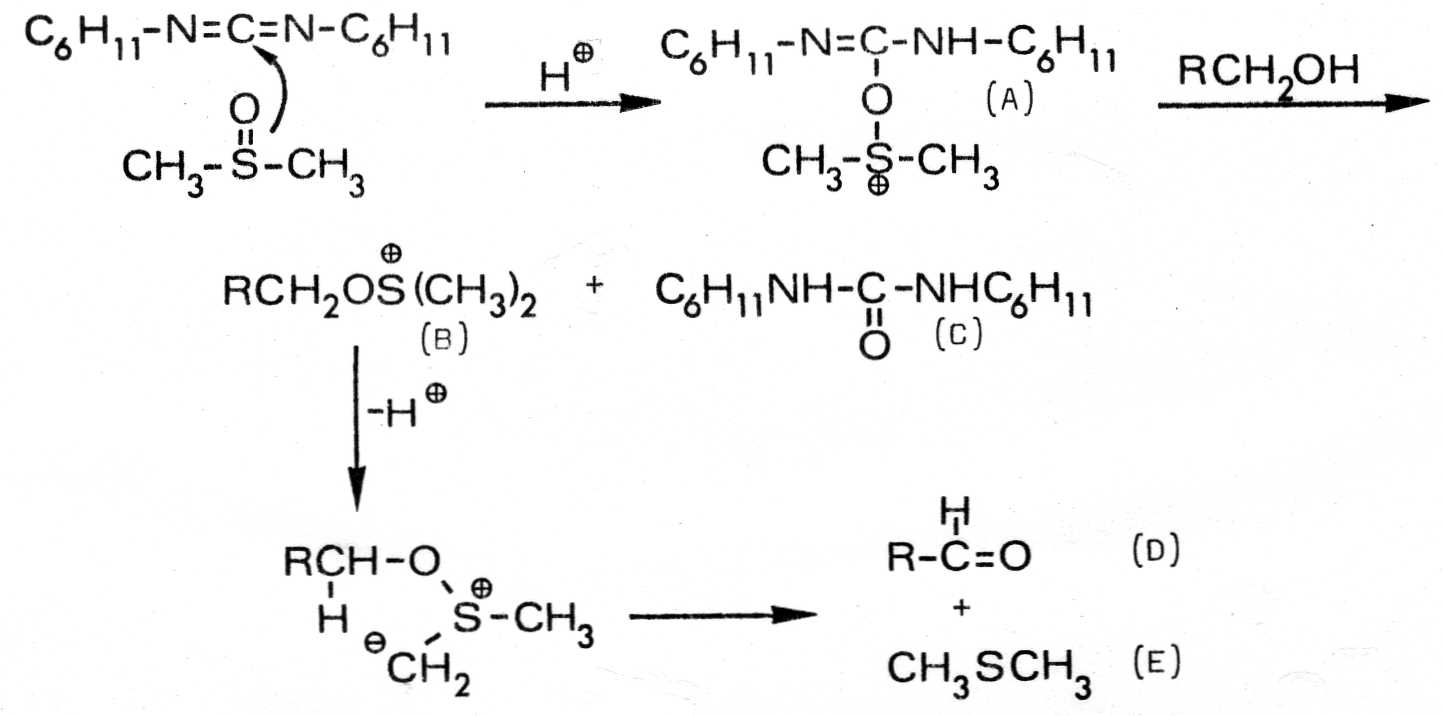
\includegraphics[width=12.217cm]{SCHEMA_001}
\begin{alltt}
Schema 1: Oxidation eines primären Alkohols mit DMSO/DCC

Das zunächst gebildete Addukt (A) reagiert mit dem Alkohol zu
einem Alkoxysulfoniumsalz (B) und zu DicyclohexylharnstoFf (C).
Unter Verlust eines Protons entsteht aus Verbindung (B) über
einen cyclischen Übergangszustand die Carbonylverbindung (D)
und Dimethylsulfid (E).

J. D. Albright und L. Goldman ersetzten das Carbodiimid und den
Protonendonator durch Essigsäureanhydrid \raise0.5ex\hbox{[70]}. Mit dieser neuen
Kombination gelang es, das labile Alkaloid Yohimbin und andere
Indol-Alkaloide in guten Ausbeuten zu den entsprechenden Ketonen
zu oxidieren.

\end{alltt}
\hspace*{0.5cm}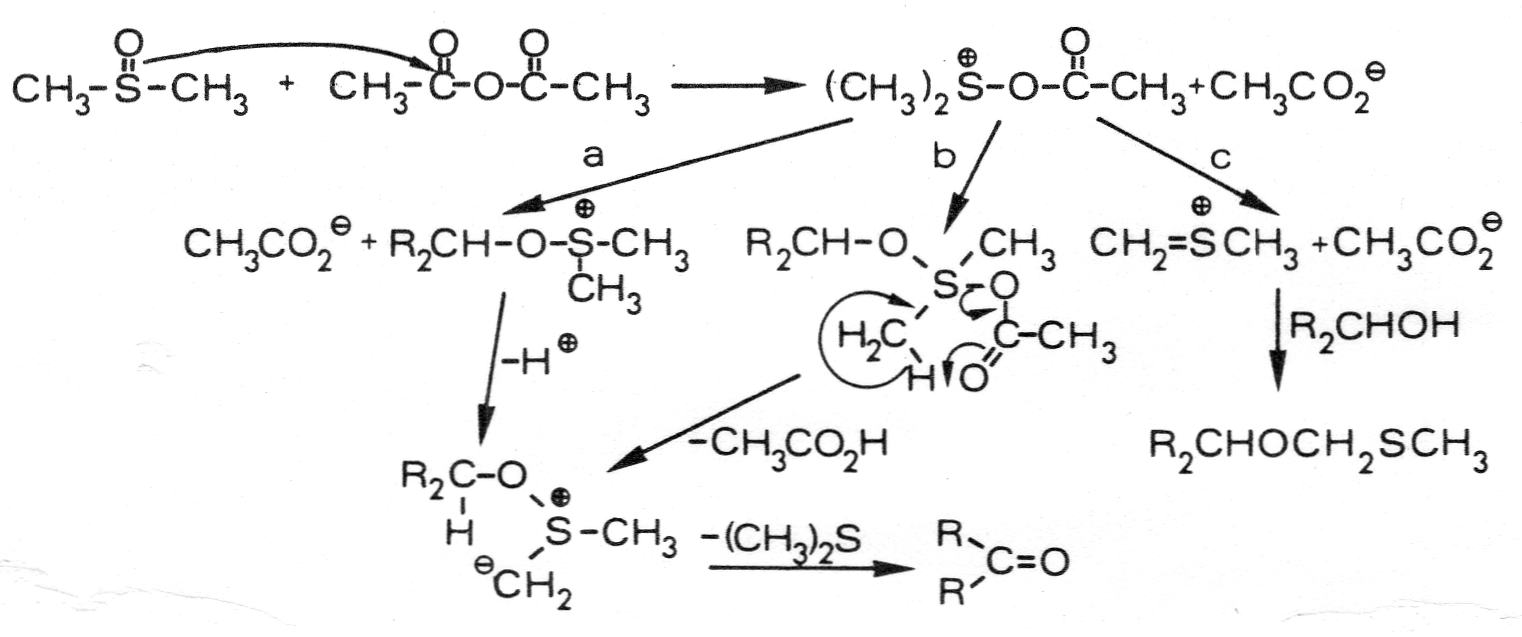
\includegraphics[width=12.886cm]{SCHEMA_002}
\begin{alltt}
Schema 2: Oxidation eines sekundären Alkohols mit DMSO/Acetanhydrid

\newpage
\makebox[0.8\textwidth][c]{- 24 -}


Die Oxidation verläuft nach einem völlig analogen Mechanismus: Das
zunächst gebildete Additionsprodukt reagiert alternativ über Weg a
oder b zur Carbonylverbindung ab, es besteht jedoch die Gefahr von
Nebenreaktionen, da über Weg c leicht Thiomethoxymethyläther ent-
stehen können.

\end{alltt}
\schemestart
\hspace{0.5cm}
% 11-Hydroxy-1,6-methano-[10]annulen (20)
\chemname{
\chemfig{=_[:60]-[:12]=_[:-12]
(-[:-252]?(-[:15]OH))% 1,6 Brücke
-[:12]=_[:-12]-[:-120]=_[:-168]-[:168]?=_[:-168]-[:168]}
}{\cmpd{hydoxymethano10annulen}}
\arrow(.mid east--.mid west){->[\textsf{\raise1.5pt\hbox{DMSO}}][\chemfig{Ac_2O}]}
% 11-Methylhiomethoxy-1,6-methano-[10]annulen (39)
\chemname{
\chemfig{=_[:60]-[:12]=_[:-12]
(-[:-252]?(-[:15]OCH_2SCH_3))% 1,6 Brücke
-[:12]=_[:-12]-[:-120]=_[:-168]-[:168]?=_[:-168]-[:168]}
}{\cmpd{thioethermethano10annulen}}
% 11-Oxo-1,6-Methano-[10]annulen (15)
\chemname{
\chemfig{=_[:60]-[:12]=_[:-12]
(-[:-252]?(=[:90,0.6]O))% 1,6 Brücke
-[:12]=_[:-12]-[:-120]=_[:-168]-[:168]?=_[:-168]-[:168]}
}{\cmpd{hexaentroponophan}}
\schemestop
\chemnameinit{}
\begin{alltt}

Eine erste Umsetzung des Alkohols (20) mit Dimethylsulfoxid/Essig-
säureanhydrid erbrachte sogleich den Beweis Für die Wirksamkeit
des neuen Reagens. Nach viertägigem Stehen bei Raumtemperatur
hatte sich das Edukt (20) vollständig umgesetzt; dünnschichtchro-
metographisch (SiO\lower0.5ex\hbox{2}/CHCl\lower0.5ex\hbox{3}) ließen sich zwei eng zusammenlaufende
Produkte nachweisen, die durch Säulenchromatographie an Kieselgel
(Eluens: Chloroform) aufgetrennt wurden. Die erste Komponente fiel
in 46 \%iger Ausbeute als hellgelbe Nadeln vom Schmelzpunkt 83 -
85\degree{}C an.

\end{alltt}
\hspace*{-0.25cm}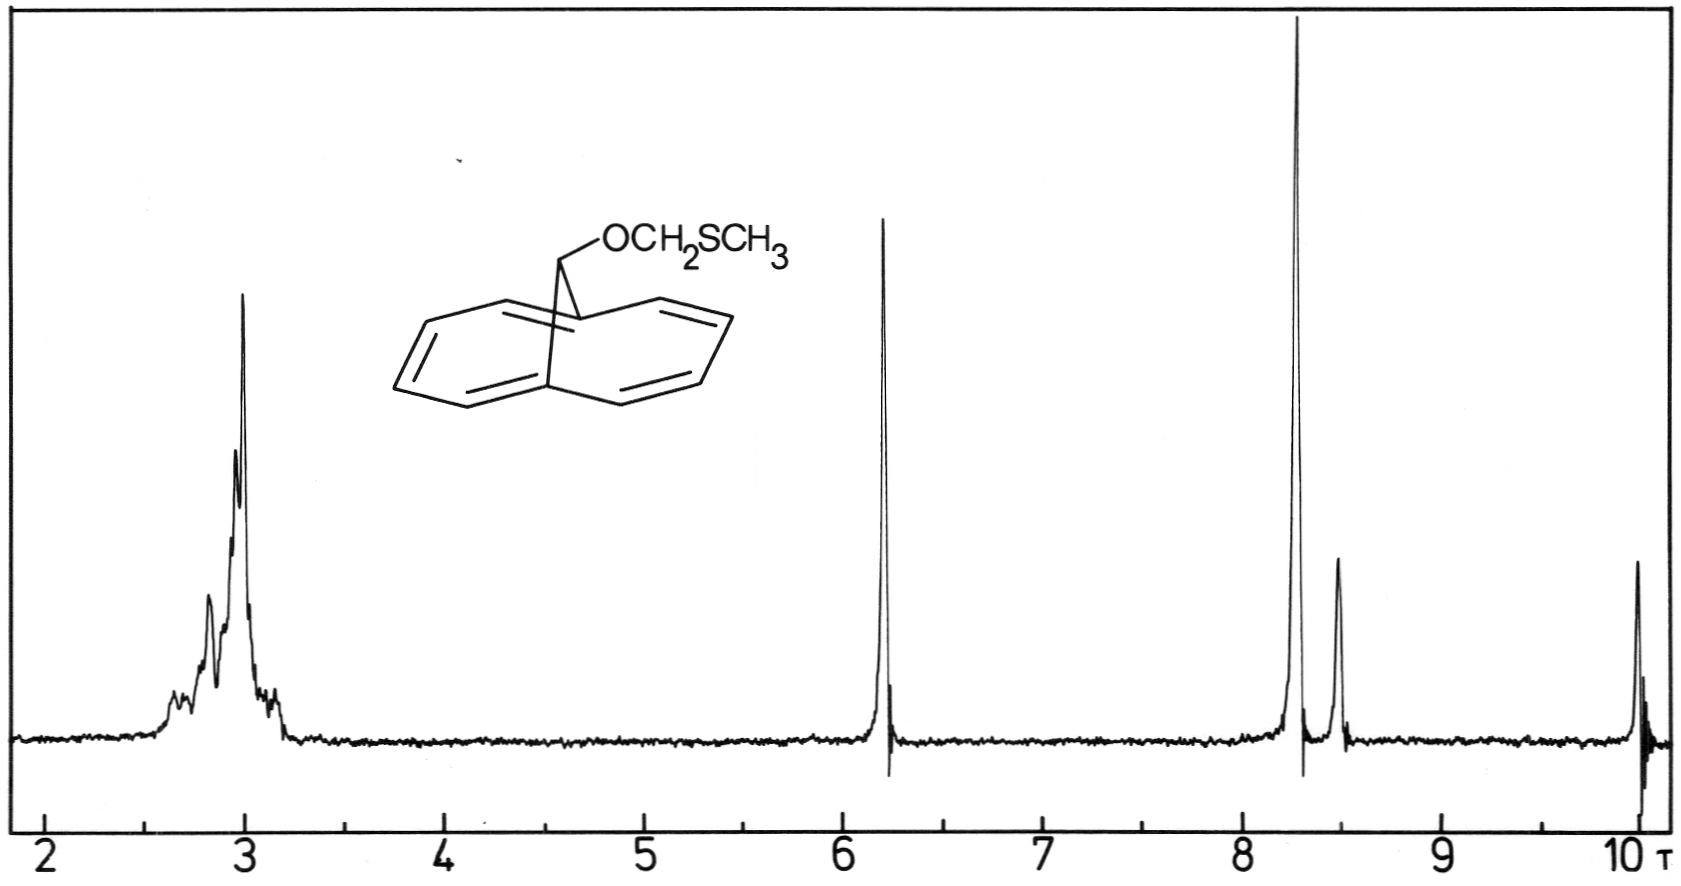
\includegraphics[width=14.23cm]{NMR_009}
\begin{alltt}
Abb. 9: \raise0.5ex\hbox{1}H-NMR-Spektrum des 11-Thiomethoxymethyl-1,6-methano-
[10]annulens (39) in CCl\lower0.5ex\hbox{4} (60 MHz; TMS als innerer
Standard)

\newpage
\makebox[0.8\textwidth][c]{- 25 -}


Das \raise0.5ex\hbox{1}H-NMR-Spektrum weist das Molekül als 11-Thiomethoxymethyl-
1,6-methano-[10]annulen (39) aus. Die Perimeterprotonen geben das
übliche Multiplett bei \(\tau\) = 2.43 - 3.25, und das Brückenproton H-11
absorbiert bei \(\tau\) = 8.50, während sich der neue Substituent durch
Singuletts bei \(\tau\) = 6.20 (2 Methylenprotonen) sowie bei \(\tau\) = 8.27
(Methylgruppe) zu erkennen gibt.

Das Auftreten des nach Reaktionsschema 2 zu erwartenden Nebenpro-
duktes (39) lässt für eine Entstehung des Ketons (15) hoffen. Tat-
sächlich erweist sich die zweite Fraktion als das lang gesuchte
11-Oxo-1,6-methano-[10]annulen (15). Man isoliert gelbgrüne
Kristallblättchen mit dem ungewöhnlich hohen Schmelzpunkt von
185 - 186\degree{}C, die sich unzersetzt im Hochvakuum sublimieren lassen.

Da die Ausbeute an Keton (15) nur 35 \% für das Rohprodukt beträgt,
sind zunächst systematische Versuche zur Optimierung der Oxidation
erforderlich. Dabei stellt sich heraus, daß die besten Ergebnisse
mit einer Vorschrift aus der Steroidchemie \raise0.5ex\hbox{[71]} erzielt werden,
die die Verwendung von DMSO in Gegenwart von Dicyclohexylcarbo-
diimid und Pyridin-trifluoracetat (PTFA) vorsieht. Nach zwei-
tägiger Reaktionsdauer erhält man in 64 \%iger Ausbeute bereits
reines Keton (15), das nach zweimaligem Umkristallisieren aus
Methanol den konstanten Schmelzpunkt von 188 - 189\degree{}C aufWeist.

Als ausgesprochen störend bei der wässrig-ätherischen Aufarbeitung
erweist sich der Dicyclohexylharnstoff. Wegen seiner Schwerlös-
lichkeit lässt er sich zwar durch Filtration entfernen, ein nicht
geringer Anteil bleibt jedoch in der organischen Phase zurück, was
die Reindarstellung des Ketons (15) ungemein erschwert, da er
selbst durch Säulenchromatographie nicht abgetrennt wird. J. G.
Moffat \raise0.5ex\hbox{[72]} schlägt in diesem Fall die Verwendung von Diäthylcarbo-
diimid vor, da dieses einen wasserlöslichen Harnstoff bildet.
Ähnlich hinderlich ist auch der große Überschuss an Dicyclohexyl-
carbodiimid selbst, das allerdings durch Digerieren mit Pentan, in
dem das Keton (15) relativ schwer löslich ist, entfernt werden
kann. Literaturrecherchen ergaben, daß in der Peptidchemie ver-
wandte Probleme anstehen: Als Kondensationsmittel zum Knüpfen der
\newpage
\makebox[0.8\textwidth][c]{- 26 -}


Peptidbindungen dienten hier zunächst Diisopropyl- und Dicyclo-
hexylcarbodiimid \raise0.5ex\hbox{[73]}. Die entsprechenden Harnstoffe besitzen
jedoch den Peptiden ähnliche Löslichkeiten, so daß man dazu über-
ging, speziell für diesen Zweck synthetisierte wasserlösliche
Carbodiimide \raise0.5ex\hbox{[74]} einzusetzen. Als besonders wirksam wurde das
Äthyl-[3-(dimethylamino)propyl]carbodiimid-hydrochlorid (40) her-
ausgestelltt \raise0.5ex\hbox{[75]}.

\end{alltt}
\hspace{3cm}
% Amino-carbodiimid (40)
\chemname{
\chemfig{CH_3CH_2{-}N{=}C{=}N{-(}CH_2{)}_3\chemabove[0.5pt]{N}{\scriptstyle\oplus}H{(}CH_3{)}_2{\ }Cl^{\ominus}}
}{\cmpd{aminocarbodiimid}}
\begin{alltt}

Die Übertragung dieses etwas exotischen Reagens' auf die Oxidation
des Alkohols (20) erbringt exzellente Resultate. Die wässrig-
ätherische Aufarbeitung gestaltet sich gänzlich unproblematisch,
da die ätherische Schicht nach dreimaligem Ausschütteln mit Wasser
nur noch das gewünschte Keton (15) enthält, das nach Abziehen des
Lösungsmittels sofort kristallin in praktisch quantitativer Aus-
beute anfällt.

In der Kombination DMSO/Äthyl-[3-(dimethylamino)propyl]carbodiimid-
hydrochlorid/PTFA steht somit ein effizientes Oxidationsmittel auch
für sterisch gehinderte oder labile Alkohole zur Verfügung, das
sich durch hohe Selektivität, Anwendbarkeit unter schonenden Bedin-
gungen (Raumtemperatur, Neutralbereich) sowie maximalen Wirkungs-
grad auszeichnet.

2.1.3 Spektrale Parameter des 11-Oxo-1,6-methano-[10]annulen (15)

Die spektralen Daten der Verbindung (15) sprechen für ein aroma-
tisches Molekül, das außerdem eine aliphatische Ketogruppe enthält.
So tritt im IR-Spektrum bei 1740 cm\raise0.5ex\hbox{-1} eine starke Carbonylbande
auf. Die hohe Frequenz dieser Schwingung entspricht normalerweise
den Werten für Fünfringketone, deutet in diesem Fall also auf einen
Bindungswinkel C1-C11-C6 von etwa 108\degree hin, da ein enger Zusammen-
hang zwischen IR-Carbonylfrequenz und Ringgröße besteht \raise0.5ex\hbox{[76]}. Ein
Konjugationseinfluß des 10\(\pi\)-Elektronensystems läßt sich anhand
dieses Wertes zwar nicht ausschließen, aber auch nicht beweisen, da
\newpage
\makebox[0.8\textwidth][c]{- 27 -}


dann die Frequenz merklich tiefer liegen müsste. Eine endgültige
Klärung dieser Frage wird im folgenden Kapitel versucht. Der C-H -
Schwingungsbereich wird bei 3065 cm\raise0.5ex\hbox{-1} und 3030 cm\raise0.5ex\hbox{-1} nur von Banden
geprägt, die der Gruppierung C=C-H zugeordnet werden müssen.

\end{alltt}
\hspace*{-0.2cm}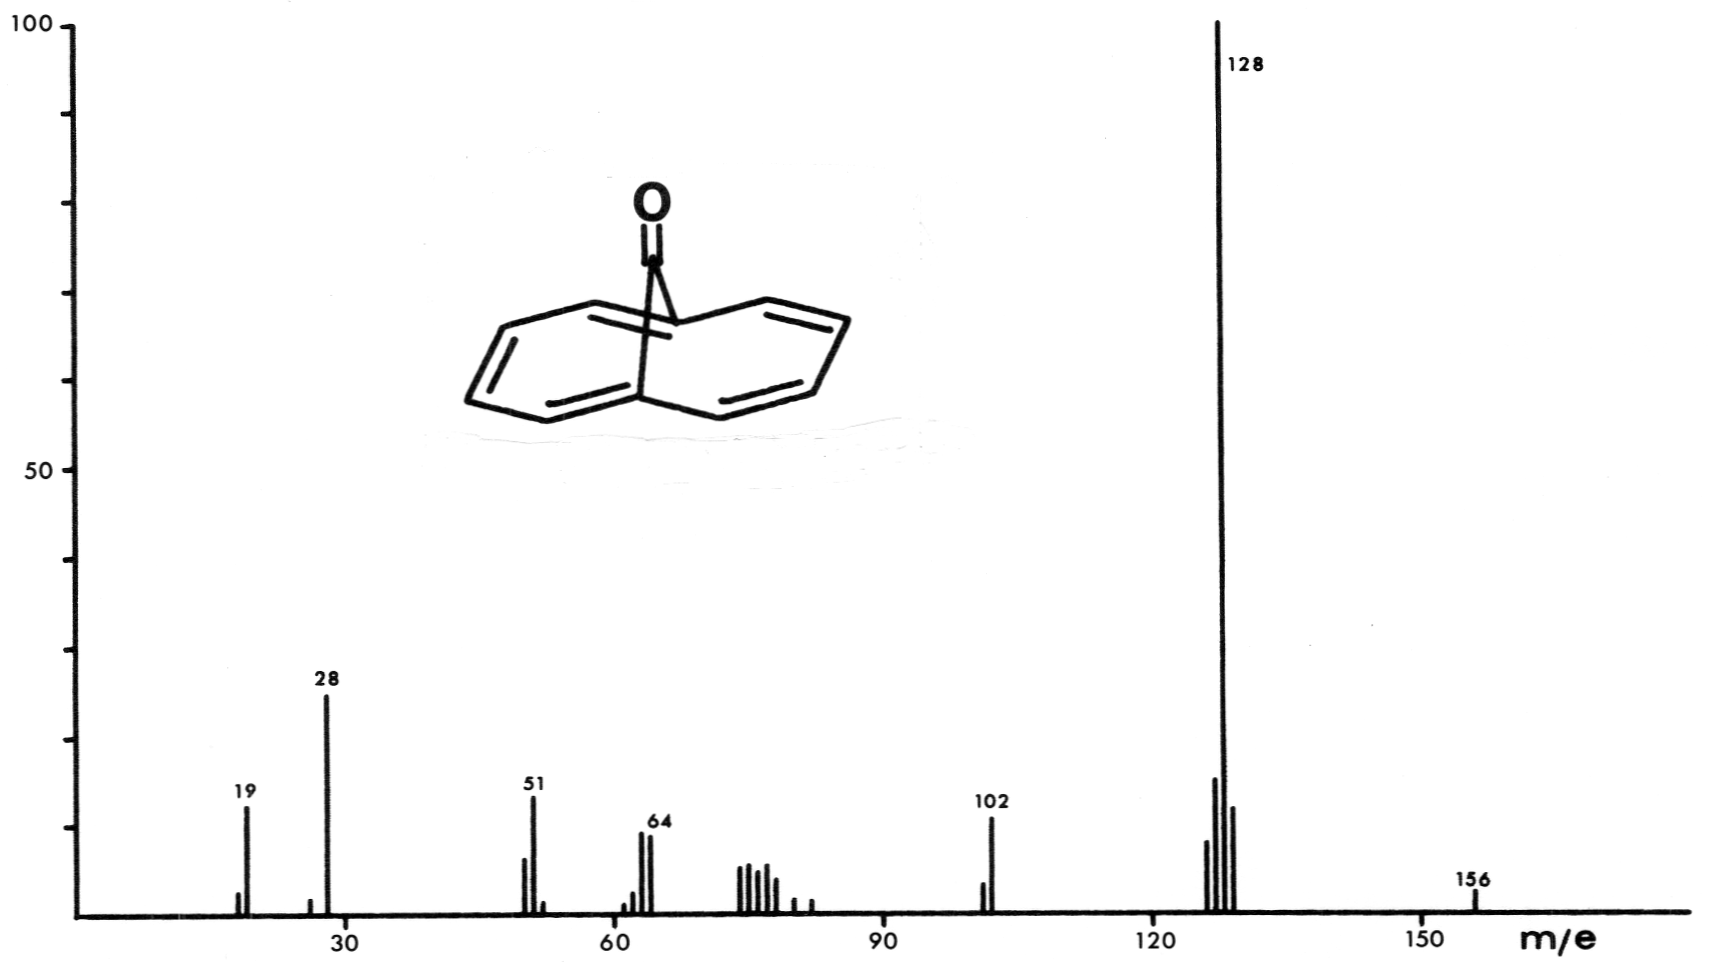
\includegraphics[width=14.487cm]{MASS_010}
\begin{alltt}
Abb. 10: Massenspektrum des 11-Oxo-1,6-methano-[10]annulens (15)
(100 eV)

Das Keton (15) zeigt im Massenspektrum einen für [10]Annulene unüb-
lichen Fragmentierungsverlauf. Während beim 1,6-Methano-[10]annulen
(16) der Massenpeak bei m/e = 141 (Benzotropyliumion) domi-
niert \raise0.5ex\hbox{[77]}, wird hier als primärer ZerfallsprozeB die Abspaltung
von Kohlenmonoxid favorisiert. Der außergewöhnlich kleine Molekül-
peak (rel. Int. 3 \%) bei m/e = 156 wird überragt durch den Basis-
peak bei m/e = 128 für das Naphthalinradikalkation, dessen weiterer
Zerfall \raise0.5ex\hbox{[78]} das Spektrum bestimmt. Ähnliche Verhältnisse im elek-
tronenstoß-induzierten Zerfall wurden für Tropon [79] und das Benz-
tropon \raise0.5ex\hbox{[80]} publiziert. Auch bei den an C-11 dihalogen-substituier-
ten [10]Annulenen sind im Massenspektrum ähnliche Intensitäten für
den Peak m/e = 128 zu beobachten, da sich diese Verbindungen unter
Carbenabspaltung zu Naphthalin stabilisieren \raise0.5ex\hbox{[77]}.

\newpage
\makebox[0.8\textwidth][c]{- 28 -}

\end{alltt}
\hspace*{-0.25cm}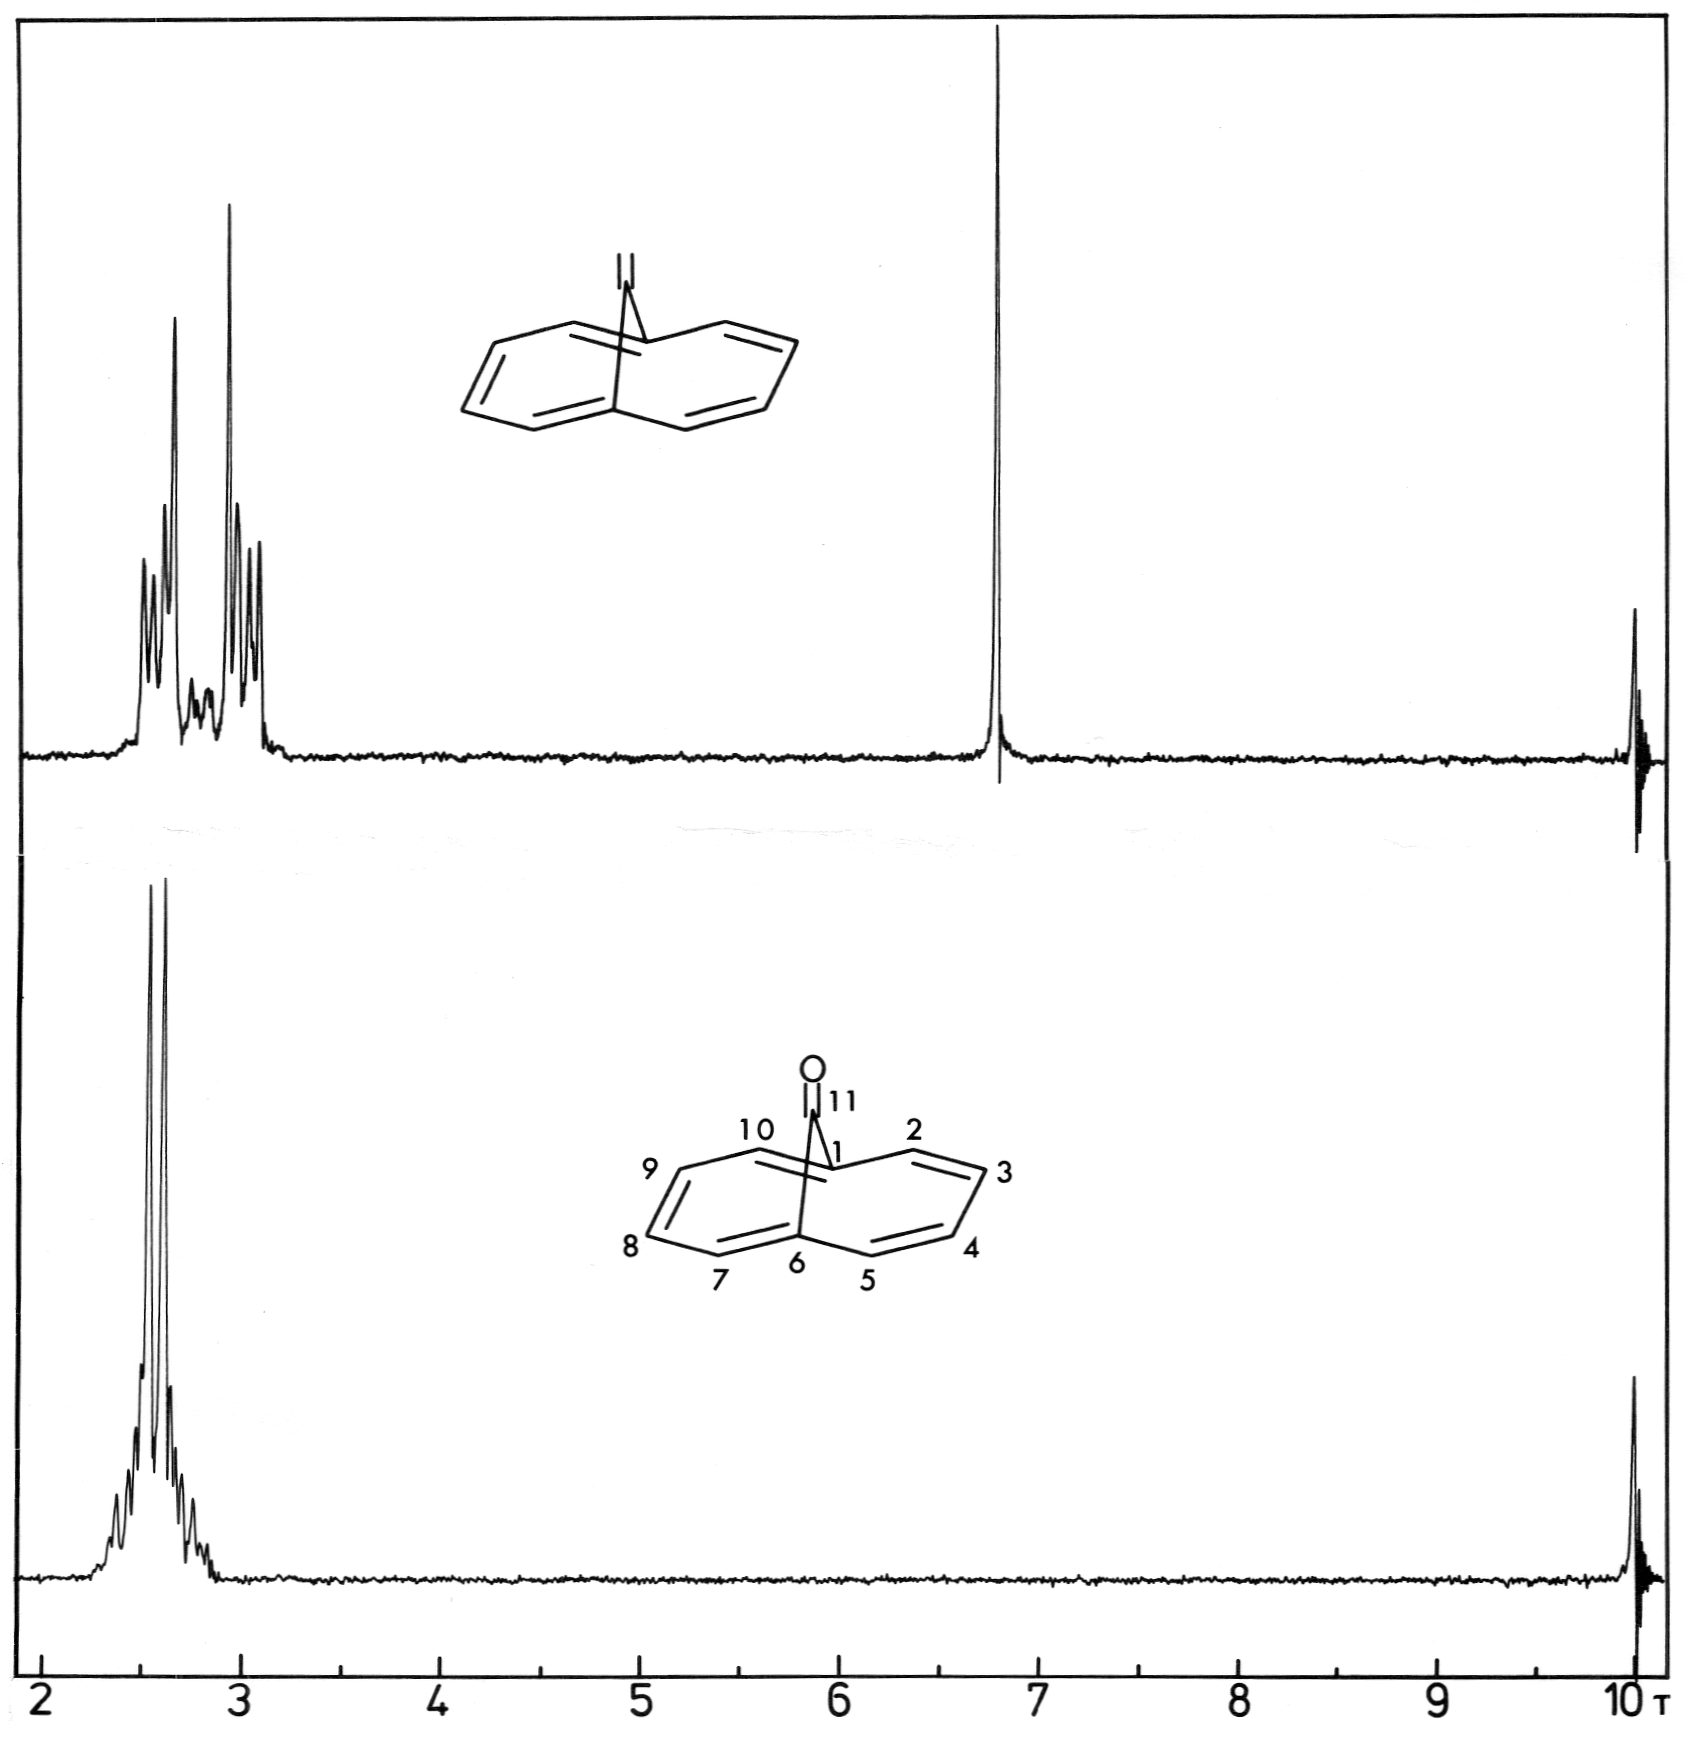
\includegraphics[width=14.283cm]{NMR_011}
\begin{alltt}
Abb. 11: \raise0.5ex\hbox{1}H-NMR-Spektren des 11-Methylen-1,6-methano-[10]annulens
(17) in CCl\lower0.5ex\hbox{4} und des 11-0xo-1,6-methano-[10]annulens (15)
in CDCl\lower0.5ex\hbox{3} (60 MHz; TMS als innerer Standard)

 

Das \raise0.5ex\hbox{1}H-NMR-Spektrum ist mit der Struktur des Ketons (15) in Ein-
klang. Zentriert bei \(\tau\) = 2.55 erscheint ein im Vergleich zum
11-Methylen-1,6-methano-[10]annulen (17) sehr enges AA'BB'-System.
Eine erneute Aufnahme des Spektrums des 11-Oxo-1,6-methano-
[10]annulens in Trifluoressigsäure ergibt keine Änderung des
Signalcharakters oder der Absorptionslage, so daß die Bildung
eines Kations auszuschließen ist.

\newpage
\makebox[0.8\textwidth][c]{- 29 -}


War das \raise0.5ex\hbox{1}H-NMR-Spektrum wenig aussagekräftig, so sollte das \raise0.5ex\hbox{13}C-
NMR-Spektrum einen differenzierteren Einblick in die struk-
turelle Beschaffenheit des Ketons (15) liefern. Auf Grund der
geringen Intensität und der tiefen Absorptionslage ist das Signal
bei \(\delta\) = 197.4 ppm dem an den Sauerstoff gebundenen Brückenkohlen-
stoff C-11 zuzuweisen. Die Resonanzfrequenz entspricht etwa der

\end{alltt}
\hspace*{-0.25cm}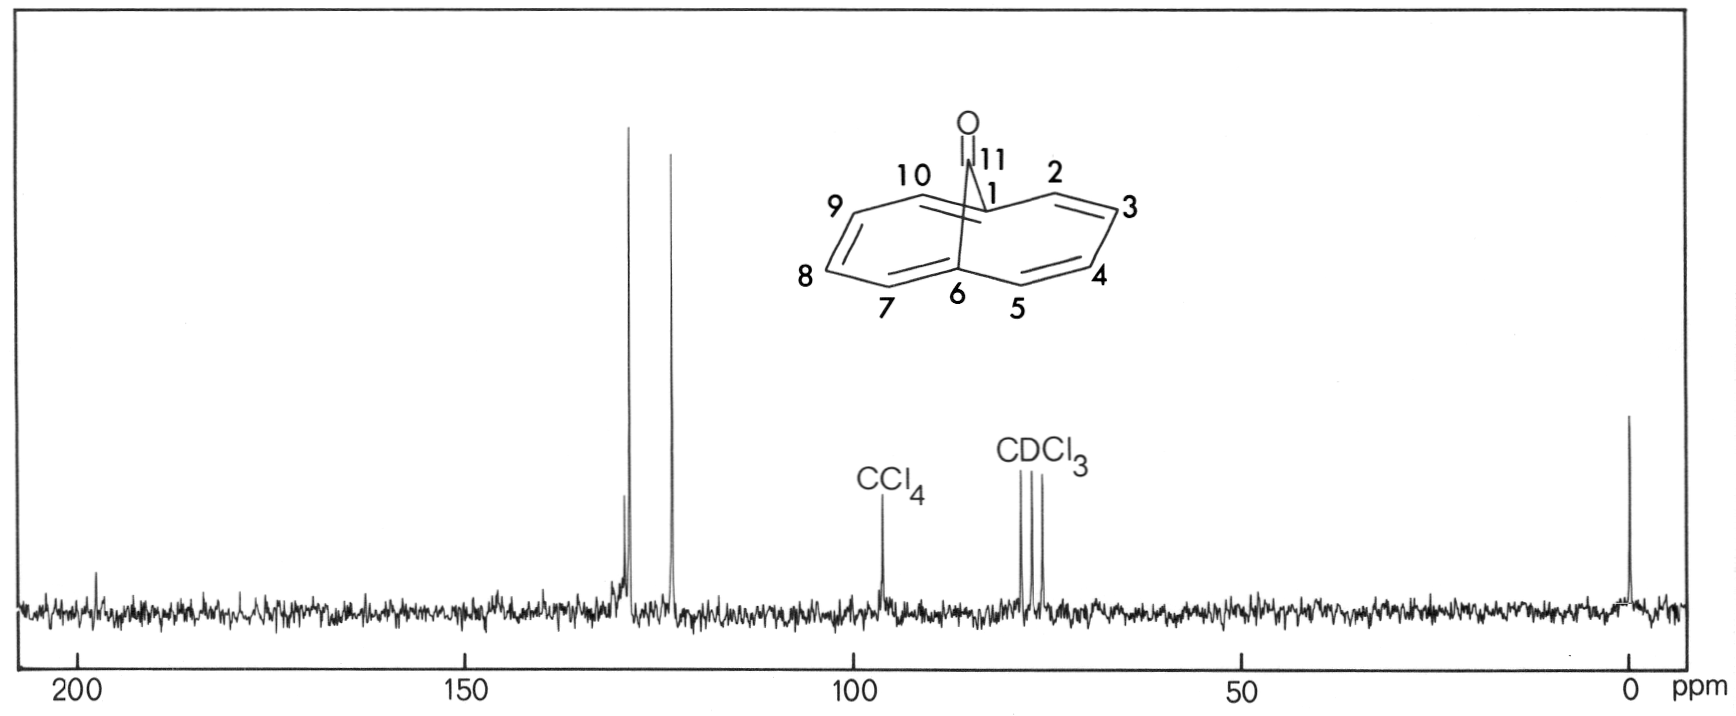
\includegraphics[width=14.7cm]{NMR_012}
\begin{alltt}
Abb. 12: \raise0.5ex\hbox{13}C-NMR-Spektrum des 11-Oxo-1‚6-methano-[10]annulens (15)
in CCl\lower0.5ex\hbox{4}/CDCl\lower0.5ex\hbox{3} 3:1 (22.63 MHz; rauschentkoppelt; TMS als
innerer Standard; Lockfrequenz: \raise0.5ex\hbox{2}H-Resonanz des CDCl\lower0.5ex\hbox{3})

im Cyclohexen-2-on-1 \raise0.5ex\hbox{[81]}. Erst die zusätzliche Registrierung eines
unentkoppelten Spektrums erlaubt die Identifizierung der Perimeter-
kohlenstoffe. Wie im Falle des 1,6-Methano-[10]annulens (16), bei
dem die entsprechenden Resonanzen durch spezifische Deuterierung
der \(\alpha\)-Stellung zugeordnet werden konnten, beobachtet man analog
charakteristische "fingerprints" \raise0.5ex\hbox{[82]}, die ohne große Mühe eine
eindeutige Festlegung der Resonanzfrequenzen für die \(\alpha\)- bzw. \(\beta\)-
Position bei \(\delta\) = 123.3 sowie 128.7 ppm erlauben. Die Brückenbasis-
atome C-1 und C-6 absorbieren fast 15 ppm höher als im 1,6-Methano-
[10]annulen (16). Mit 129.4 ppm stellt diese Frequenz den höchsten
bisher für ein 1,6-Methano-[10]annulen-Derivat gemessenen Wert dar.
Er ist vergleichbar mit entsprechenden Absorptionen beim 1,6-Oxido-
[10]annulen (\(\delta\) = 131.2 ppm) und Naphthalin (\(\delta\) = 133.4 ppm) \raise0.5ex\hbox{[83]} und
spricht damit für eine hohe Einebnung des Kohlenstoffgerüstes.

Diese Schlussfolgerung wird durch die Aufnahme eines ESR-Spektrums
noch erhärtet \raise0.5ex\hbox{[84]}. Nach der Hückel-Molecular-Orbital-Theorie \raise0.5ex\hbox{[85]}

\newpage
\makebox[0.8\textwidth][c]{- 30 -}


\end{alltt}
\hspace*{-0.25cm}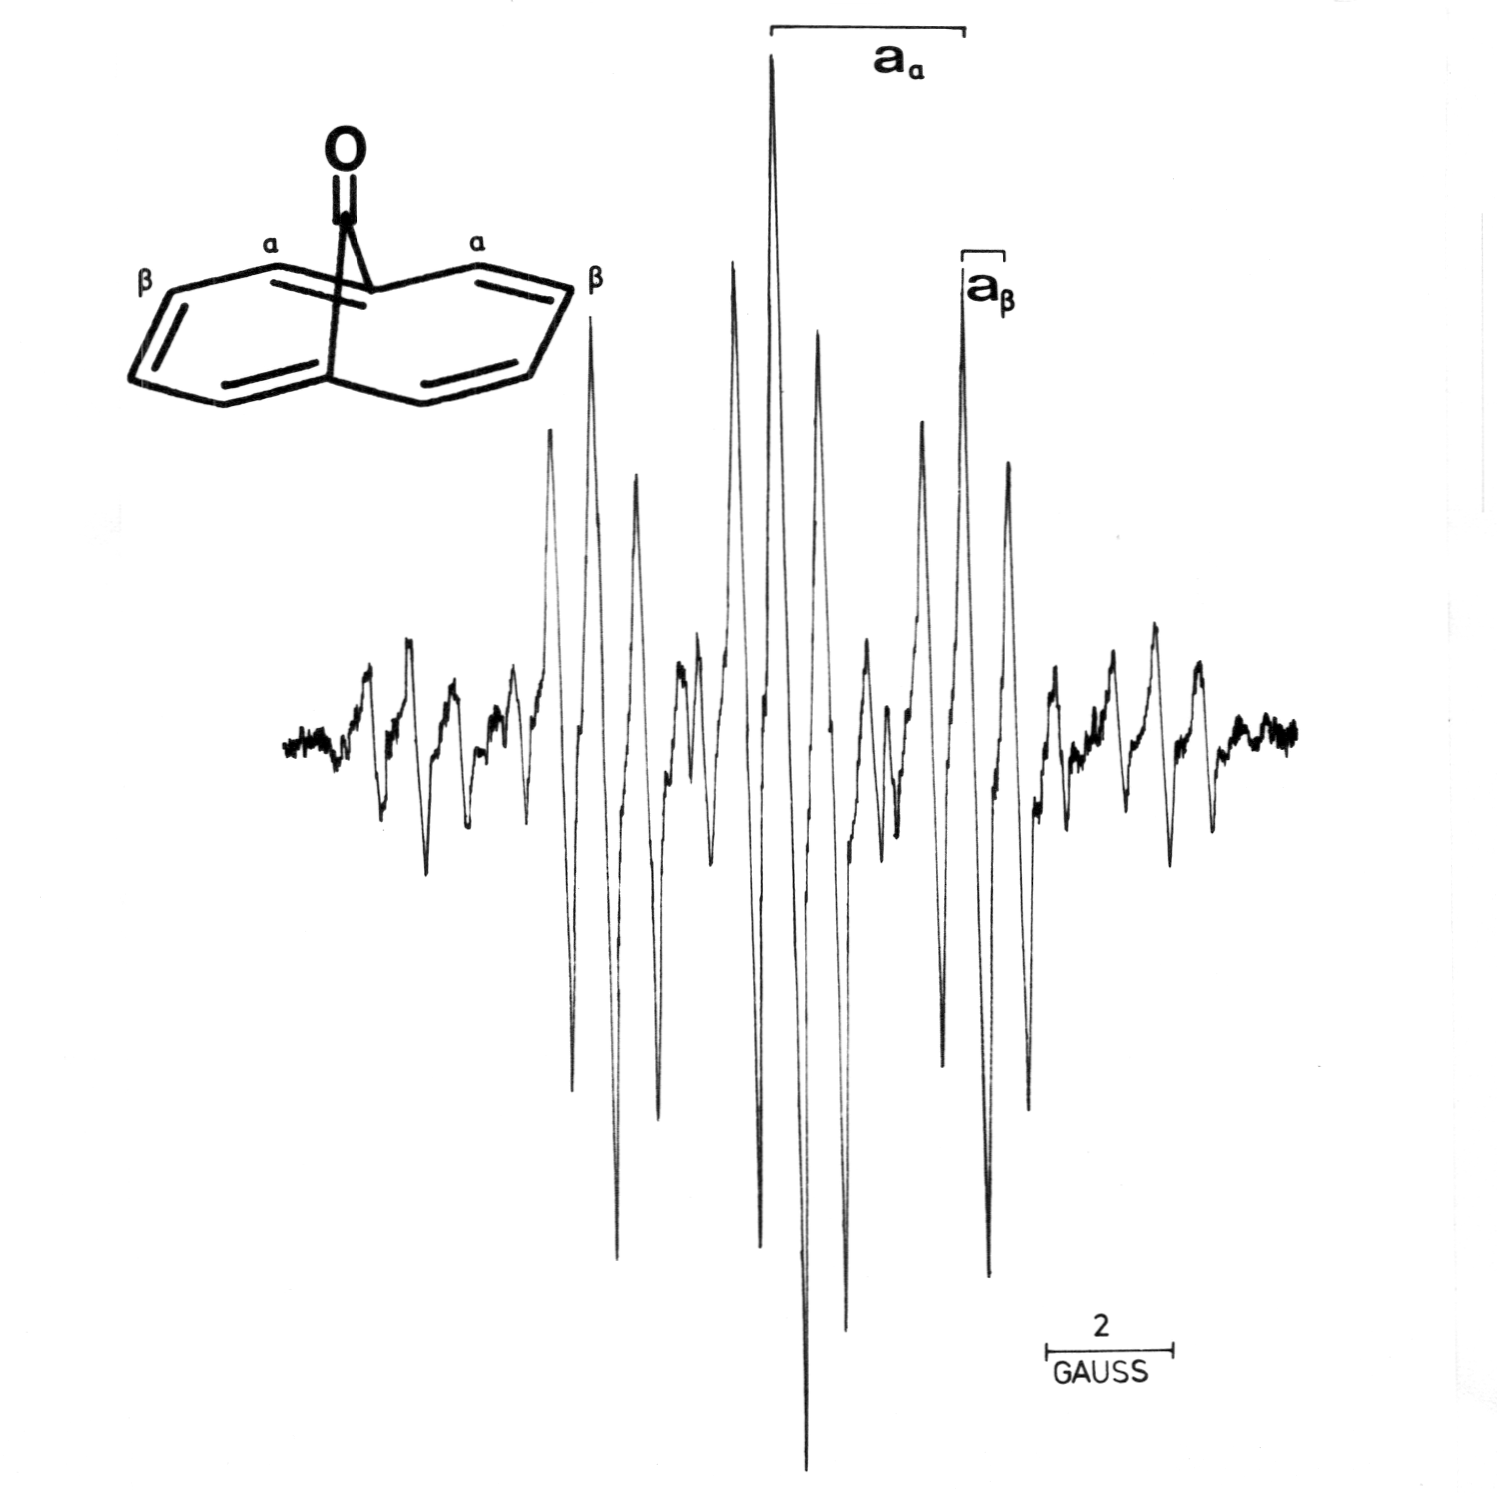
\includegraphics[width=12.675cm]{ESR_013}
\begin{alltt}
Abb. 13: ESR-Spektrum des 11-Oxo-1‚6-methano-[10]annulens (15),
0.002 m in DMF (-60\degree{}C; Leitsalz: 0.1 m Tetraäthyl-
ammoniumperchlorat)

lassen sich die Hyperfeinkopplungskonstanten a\(\mu\) mit der McConnell'
schen Gleichung \raise0.5ex\hbox{[86]} berechnen:

\makebox[0.8\textwidth][c]{a\(\mu\) = |Q|\(\rho\mu\)}

In dieser Formel bedeutet \(\rho\mu\)  die Spinpopulation an den beteiligten
Atomen, die Größe Q ist der Elektronen-Aufenthaltswahrscheinlich-
keit am Ort des Kerns proportional. Während |Q| beim Naphthalin
dem theoretisch vorhergesagten Wert von 23 Gauss entspricht, wurden
für des 1,6-Methano-[10]annulen (16) bzw. das 1,6-Oxido-[10]annulen
empirisch nur 10 sowie 13 Gauss ermittelt. Der Proportionalitäts-
Faktor erweist sich nämlich als abhängig von der Koplanarität des
\(\pi\)-Elektronensystems und bietet eine empfindliche Sonde auf

\newpage
\makebox[0.8\textwidth][c]{- 31 -}


gestörte Orthogonalität zwischen \(\sigma\)- und \(\pi\)-Orbitalen \raise0.5ex\hbox{[87]}. Mit den
gemessenen Kopplungskonstanten a\(\alpha\) = 3.02 Gauss und a\(\beta\) = 0.69 Gauss
errechnet sich ein |Q|-Wert von etwa 11 Gauss, so daß das Keton
(15) bezüglich der Perimetergeometrie eine Mittelstellung zwischen
1,6-Methano- und 1,6-Oxido-[10]annulen einnehmen dürfte.


2.1.4 Spektroskopische Eigenschaften des 11-Oxo-1‚6-methano-
[10]annulens (15) in vergleichender Diskussion

Um weitere Aussagen über die Molekülstruktur des Ketons (15)
machen zu können, seien im Folgenden die spektroskopischen Daten
denen von ähnlichen [10]Annulenen mit verschiedenen "Brücken"
gegenübergestellt.


2.1.4.1 \raise0.5ex\hbox{13}C-NMR-Spektren-Vergleich

Anhand von Tabelle 1 (s. S. 32) wird die starke strukturelle Ver-
wandtschaft aller aufgeführten Verbindungen sofort sichtbar. Die
Resonanzen für C-2,5 sowie C-3,4 liegen jeweils in vergleichbarer
Größenordnung. Einzig in den Absorptionen für die Kohlenstoffatome
C-1 und C-6 ist ein deutlicher Trend zu beobachten. Von oben nach
unten werden die Resonanzfrequenzen immer weiter nach tieferem
Feld verschoben. In dieser Tatsache dokumentiert sich der steigende
p-Charakter in den exocyclischen Bindungen an C-11. Hauptsächlich
führt jedoch die zunehmende Spreizung des Winkels C1-C11-C6 durch
die unterschiedliche Überbrückung zu einer Abstandsvergrößerung
zwischen den Brückenbasisatomen, wodurch im Perimeter die Überlap-
pung der \(\pi\)-Orbitale infolge der zunehmenden Aufrichtung der p\lower0.5ex\hbox{z} -
Orbitale an den Zentren C-1 bzw. C-6 und der damit verbundenen
Einebnung verbessert wird. Naphthalin (21) stellt den Extremfall
der angeführten Reihe dar, hier stehen sämtliche p\lower0.5ex\hbox{z} - Orbitale
parallel zueinander. Die Vertauschung der Frequenzen für die \(\alpha\)-
und \(\beta\)-Position im Keton (15) und Äther (42) scheint ohne tiefere

\newpage
\makebox[0.8\textwidth][c]{- 32 -}

\end{alltt}
\begin{table}[h!]\ttfamily
\captionsetup{singlelinecheck = false, justification=justified, labelfont=tt, textfont=tt}
\caption[caption]
    {\tabular[t]{@{}l@{}}\raise0.5ex\hbox{13}C-NMR-Daten einiger ausgewählter [10]Annulene\\
    (22.63 MHz; \(\delta\)-Werte in ppm; TMS als innerer Standard)\endtabular}
\label{tab:13CNMRDaten}
 \begin{tabular}{ccccccc}
 \  & \  & C-1,6  & C-2,5  & C-3,4  & C-11 & Liter.\\
% 1,6-methano-[10]annulen (16) mit Atomnummern
\pgfmathsetmacro{\currentscale}{0.8}%
\chemfig[atom style={scale=0.8}]{%
=_[:60,,,,shrtdbl={0pt}{3.5pt}]%
-[:12]%
=_[:-12]@{n1}%
(-[:-252]?)% 1,6 Brücke
-[:12]@{n2}%
=_[:-12,,,,shrtdbl={4pt}{0pt}]@{n3}%
-[:-120]@{n4}%
=_[:-168]@{n5}%
-[:168]?@{n6}%
=_[:-168,,,,shrtdbl={1pt}{2pt}]%
-[:168]%
}%
\chemmove{% with scale=0.8
    \node at (n1) [above right=-0.04 and -0.08] {\scriptsize\textsf{1}};
    \node at (n2) [above right=-0.04 and -0.08] {\scriptsize\textsf{2}};
    \node at (n3) [right=-0.04] {\scriptsize\textsf{3}};
    \node at (n4) [right=0.04] {\scriptsize\textsf{4}};
    \node at (n5) [below=-0.04] {\scriptsize\textsf{5}};
    \node at (n6) [below=-0.04] {\scriptsize\textsf{6}};
}%
 & (16) & 114.6 & 128.7 & 128.1 & 34.8 & [88]\\[21pt]
% 11-Methylen-1,6-Methano-[10]annulen (17)
\chemfig[atom style={scale=0.8}]{=_[:60,,,,shrtdbl={0pt}{3.5pt}]-[:12]=_[:-12]
(-[:-252]?(=[:90,0.5]))% 1,6 Brücke
-[:12]=_[:-12,,,,shrtdbl={4pt}{0pt}]-[:-120]=_[:-168]-[:168]?=_[:-168,,,,shrtdbl={1pt}{2pt}]-[:168]}
 & (17) & 121.8 & (127.1) & (128.7) & 137.5 & [83]\\[24pt]
% 11-Spiro-1,6-Methano-[10]annulen (41)
\chemfig[atom style={scale=0.8}]{=_[:60,,,,shrtdbl={0pt}{3.5pt}]-[:12]=_[:-12]%
(-[:-252]?(-[:42]-[:180,1.5]-[:-42]))% 1,6 Brücke
-[:12]=_[:-12,,,,shrtdbl={4pt}{0pt}]-[:-120]=_[:-168]-[:168]?=_[:-168,,,,shrtdbl={1pt}{2pt}]-[:168]}%
\cmpd*{spiromethano10annulen}%
 & (41) & 123.2 & 129.2 & 126.3 & 25.3 & [88]\\[21pt]%
% 11-Oxo-1,6-Methano-[10]annulen (15)
\chemfig[atom style={scale=0.8}]{=_[:60,,,,shrtdbl={0pt}{3.5pt}]-[:12]=_[:-12]
(-[:-252]?(=[:90,0.6]O))% 1,6 Brücke
-[:12]=_[:-12,,,,shrtdbl={4pt}{0pt}]-[:-120]=_[:-168]-[:168]?=_[:-168,,,,shrtdbl={1pt}{2pt}]-[:168]}
 & (15) & 129.4 & 123.3 & 128.7 & 197.4 & [d.A.]\\[21pt]
% 1,6-Oxido-[10]annulen (42)
\chemfig[atom style={scale=0.8}]{=_[:60,,,,shrtdbl={0pt}{3.5pt}]-[:12]=_[:-12]%
(-[:-252,0.9]O?)% 1,6 Brücke
-[:12]=_[:-12,,,,shrtdbl={4pt}{0pt}]-[:-120]=_[:-168]-[:168]?=_[:-168,,,,shrtdbl={1pt}{2pt}]-[:168]}%
\cmpd*{oxidomethano10annulen}%
 & (42) & 131.2 & 123.4 & 127.9 & --- & [83]\\[21pt]%
% Naphthalin (21) gerade
\chemfig{*6(=-@{n6}%
(*6(% Sechsring
-@{n5}%
=@{n4}%
-@{n3}%
=@{n2}%
-@{n1}%
-))=-=-)
}%
\chemmove{
    \node at (n1) [above=-0.05] {\scriptsize\textsf{1}};
    \node at (n2) [above=-0.05] {\scriptsize\textsf{2}};
    \node at (n3) [right=-0.05] {\scriptsize\textsf{3}};
    \node at (n4) [right=-0.05] {\scriptsize\textsf{4}};
    \node at (n5) [below=-0.05] {\scriptsize\textsf{5}};
    \node at (n6) [below=-0.04] {\scriptsize\textsf{6}};
}%
% reset scale to normal
\pgfmathsetmacro{\currentscale}{\normalscale}
 & (21) & 133.4 & 127.7 & 125.7 & --- & [89]\\
 \end{tabular}
\end{table}
\begin{alltt}

Bedeutung zu sein, sie ist wohl auf den Anisotrooieeffekt des
Sauerstoffatome zurückzuführen.


2.1.4.2 \raise0.5ex\hbox{1}H-NMR-Spektren-Vergleich

Die äußere Gestalt des \raise0.5ex\hbox{1}H-NMR-Spektrums (s. S. 28) deutet schon
auf ähnliche Elektronendichte-Verhältnisse wie beim 1,6-Oxido-
[10]annulen (42) \raise0.5ex\hbox{[90]} hin. Beide Verbindungen zeigen im Gegensatz
zu den anderen in Tabelle 2 (s. S. 33) aufgeführten Referenzsub-
stanzen ein sehr enges AA'BB'-System für die aromatischen Protonen.
Eine genaue Protonenanalyse wurde anhand von 100 MHz-Spektren
durchgeführt. Dazu ermittelte man aus den aufgenommenen Spektren
die chemischen Verschiebungen und Kopplungskonstanten durch direkte
Analyse \raise0.5ex\hbox{[94]} und verfeinerte die Werte iterativ mit Hilfe des
Rechenprogramms LAOCOON 3 \raise0.5ex\hbox{[95]}. Dabei wurden die Fernkopplungen
\newpage
\makebox[0.8\textwidth][c]{- 33 -}

\end{alltt}
% next from <http://tex.stackexchange.com/questions/2441/how-to-add-a-forced-line-break-inside-a-table-cell>
\newcommand{\specialcell}[2][c]{%
 \begin{tabular}[#1]{c@{}}#2\end{tabular}
}
\begin{table}[h!]\ttfamily
\captionsetup{singlelinecheck = false, justification=justified, labelfont=tt, textfont=tt}
\caption[caption]
    {\tabular[t]{@{}l@{}}\raise0.5ex\hbox{1}H-NMR-Daten einiger ausgewählter [10]Annulene\\
    (100 MHz; \(\delta\)-Werte in ppm; J in Hz; \(\nu\)\lower0.5ex\hbox{o}\(\delta\) in Hz)\endtabular}
\label{tab:1HNMRDaten}
 \hspace*{-1cm}
 \begin{tabular}{cp{0.5cm}ccccccccc}
  \  & \  & \(\delta\)\lower0.5ex\hbox{(2,5)} & \(\delta\)\lower0.5ex\hbox{(3,4)} & \(\nu\)\lower0.5ex\hbox{o}\(\delta\) &%
J\lower0.5ex\hbox{(23)} & J\lower0.5ex\hbox{(24)} & J\lower0.5ex\hbox{(25)} & J\lower0.5ex\hbox{(34)} & N & Liter.\\[8pt]
% 1,6-methano-[10]annulen (16) mit Atomnummern
\pgfmathsetmacro{\currentscale}{0.8}%
\chemfig[atom style={scale=0.8}]{%
=_[:60,,,,shrtdbl={0pt}{3.5pt}]%
-[:12]%
=_[:-12]@{n1}%
(-[:-252]?)% 1,6 Brücke
-[:12]@{n2}%
=_[:-12,,,,shrtdbl={4pt}{0pt}]@{n3}%
-[:-120]@{n4}%
=_[:-168]@{n5}%
-[:168]?@{n6}%
=_[:-168,,,,shrtdbl={1pt}{2pt}]%
-[:168]%
}%
\chemmove{% with scale=0.8
    \node at (n1) [above right=-0.04 and -0.08] {\scriptsize\textsf{1}};
    \node at (n2) [above right=-0.04 and -0.08] {\scriptsize\textsf{2}};
    \node at (n3) [right=-0.04] {\scriptsize\textsf{3}};
    \node at (n4) [right=0.04] {\scriptsize\textsf{4}};
    \node at (n5) [below=-0.04] {\scriptsize\textsf{5}};
    \node at (n6) [below=-0.04] {\scriptsize\textsf{6}};
}%
 & (16) & 7.27 & 6.95 & 32.4 & 8.97 & -0.02 & 1.46 & 9.19 & 8.95 & [91]\\[21pt]
% 11-Methylen-1,6-Methano-[10]annulen (17)
\chemfig[atom style={scale=0.8}]{=_[:60,,,,shrtdbl={0pt}{3.5pt}]-[:12]=_[:-12]
(-[:-252]?(=[:90,0.5]))% 1,6 Brücke
-[:12]=_[:-12,,,,shrtdbl={4pt}{0pt}]-[:-120]=_[:-168]-[:168]?=_[:-168,,,,shrtdbl={1pt}{2pt}]-[:168]}%
 & (17) & 7.42 & 7.02 & 40.0 & 8.97 & -0.03 & 1.26 & 9.47 & 8.84 & [92]\\[21pt]
% 11-Spiro-1,6-Methano-[10]annulen (41)
% 11-Spiro-1,6-Methano-[10]annulen (41)
\chemfig[atom style={scale=0.8}]{=_[:60,,,,shrtdbl={0pt}{3.5pt}]-[:12]=_[:-12]%
(-[:-252]?(-[:42]-[:180,1.5]-[:-42]))% 1,6 Brücke
-[:12]=_[:-12,,,,shrtdbl={4pt}{0pt}]-[:-120]=_[:-168]-[:168]?=_[:-168,,,,shrtdbl={1pt}{2pt}]-[:168]}%
\cmpd*{spiromethano10annulen}%
 & (41) & 7.48 & 7.20 & 28.0 & 9.20 & -0.30 & 1.50 & 9.10 & 8.90 & [83]\\[21pt]
% 11-Oxo-1,6-Methano-[10]annulen (15)
\chemfig[atom style={scale=0.8}]{=_[:60,,,,shrtdbl={0pt}{3.5pt}]-[:12]=_[:-12]%
(-[:-252]?(=[:90,0.6]O))% 1,6 Brücke
-[:12]=_[:-12,,,,shrtdbl={4pt}{0pt}]-[:-120]=_[:-168]-[:168]?=_[:-168,,,,shrtdbl={1pt}{2pt}]-[:168]}%
 & (15) & 7.54 & 7.36 & 18.4 &%
 \specialcell{9.18\\[-0.5ex]9.16} & \specialcell{-0.01\\[-0.5ex]-0.08} & \specialcell{0.72\\[-0.5ex]0.73} &%
 \specialcell{9.18\\[-0.5ex]9.17} & \specialcell{9.17\\[-0.5ex]9.08} & [d.A.]\\[21pt]
% 1,6-Oxido-[10]annulen (42)
\chemfig[atom style={scale=0.8}]{=_[:60,,,,shrtdbl={0pt}{3.5pt}]-[:12]=_[:-12]%
(-[:-252,0.9]O?)% 1,6 Brücke
-[:12]=_[:-12,,,,shrtdbl={4pt}{0pt}]-[:-120]=_[:-168]-[:168]?=_[:-168,,,,shrtdbl={1pt}{2pt}]-[:168]}%
\cmpd*{oxidomethano10annulen}%
 & (42) & 7.46 & 7.26 & 20.3 & 8.77 & \ 0.28 & 1.13 & 9.28 & 9.05 & [91]\\[21pt]
% Naphthalin (21) gerade
\chemfig{*6(=-@{n6}%
(*6(% Sechsring
-@{n5}%
=@{n4}%
-@{n3}%
=@{n2}%
-@{n1}%
-))=-=-)
}%
\chemmove{
    \node at (n1) [above=-0.05] {\scriptsize\textsf{1}};
    \node at (n2) [above=-0.05] {\scriptsize\textsf{2}};
    \node at (n3) [right=-0.05] {\scriptsize\textsf{3}};
    \node at (n4) [right=-0.05] {\scriptsize\textsf{4}};
    \node at (n5) [below=-0.05] {\scriptsize\textsf{5}};
    \node at (n6) [below=-0.04] {\scriptsize\textsf{6}};
}%
% reset scale to normal
\pgfmathsetmacro{\currentscale}{\normalscale}
 & (21) & 7.66 & 7.30 & 36.0 & 8.28 & \ 1.24 & 0.74 & 6.85 & 7.59 & [93]\\
  \end{tabular}
\end{table}

\begin{alltt}
zwischen den beiden Ringhälften bewusst vernachlässigt, um die Ana-
lyse als einfachen 4-Spin-Fall durchführen zu können. Aus diesem
Grund weist das mit dem erhaltenen Parametersatz simulierte \leavevmode\raise0.5ex\hbox{*})
Spektrum (s. Abb. 14 auf S. 34) nur befriedigende Übereinstimmung
mit dem Experiment auf. Die berechneten Größen (mittlerer quadra-
tischer Fehler: 0.1 Hz) können jedoch als repräsentativ für das
Spektrum bezeichnet Werden; insbesondere der N-Wert von 9.1 Hz
weist das Keton (15) eindeutig als [10]Annulen aus. Im Vergleich
zu den anderen Verbindungen in Tabelle 2 sind die beiden vicinalen
Kopplungskonstanten extrem angeglichen. Dies kann als Indiz Für
eine sehr weitgehende Bindungslängenangleichung im 11-Oxo-
1,6-methano-[10]annulen (15) gewertet werden.

\(\overline{\hspace{7cm}}\)
\leavevmode\raise0.5ex\hbox{*}) Zur Simulation des theoretischen Spektrums diente das Rechenpro-
   gramm LAOCPL (s. Kap. "Computerrechnungen").
\newpage
\makebox[0.8\textwidth][c]{- 34 -} 


\end{alltt}
\begin{minipage}{7.5cm}
  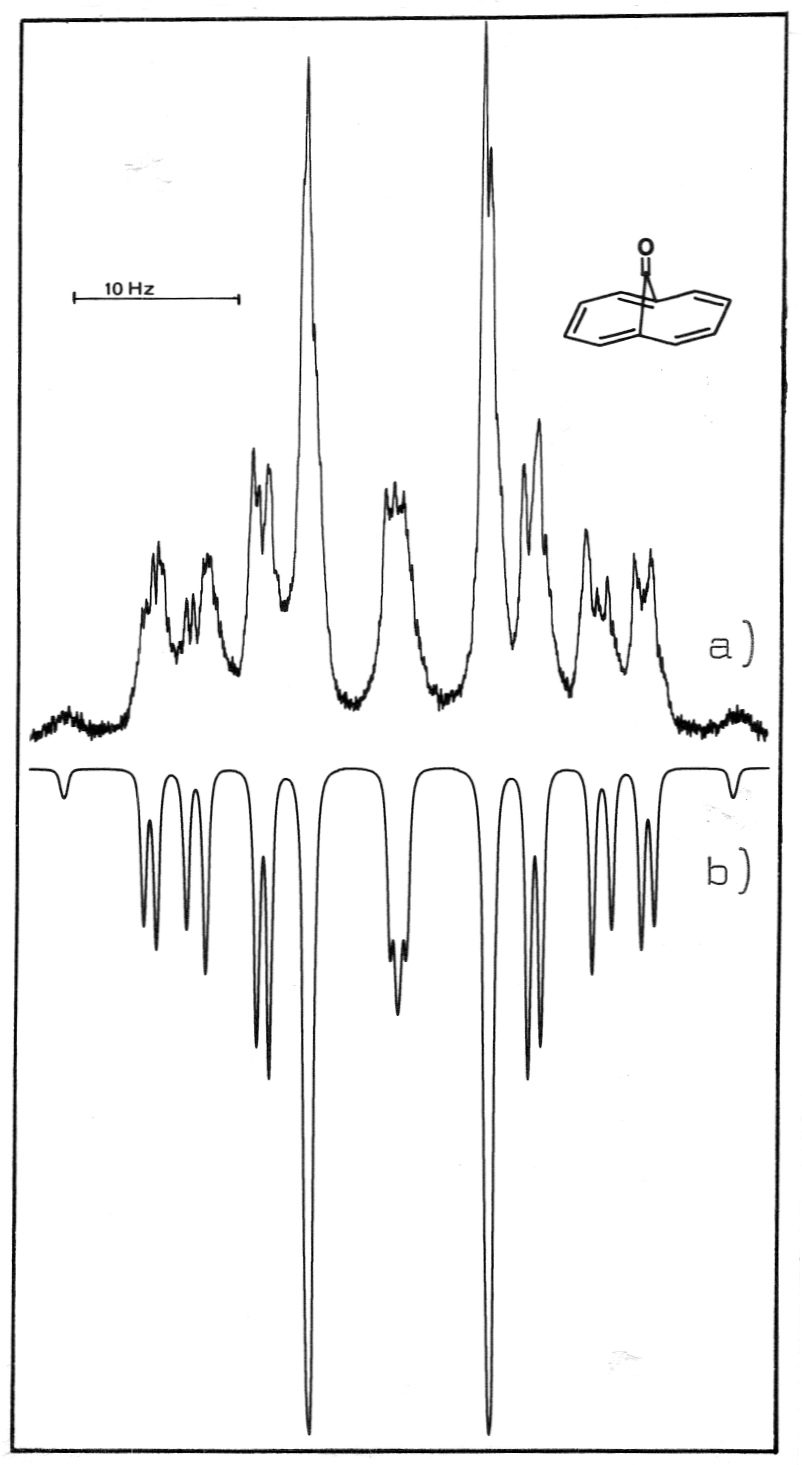
\includegraphics[width=6.79cm]{ESR_014}
\end{minipage}%
%\hfill%
\begin{minipage}{0.5\textwidth}
\begin{alltt}
Abb. 14:
Experimentelles a) und theoreti-
sches b) \raise0.5ex\hbox{1}H-NMR-Spektrum der
Perimeterprotonen des
11-Oxo-1,6-methano-[10]annulens
(100 MHz; 100 Hz sweep width)
\end{alltt}
\end{minipage}
\begin{alltt}



2.1.4.3 UV-Spektren-Vergleich

Das Keton (15) zeigt im Ultraviolettabsorptionsspektrum (s. Abb. 15
auf s. 35) mit \(\lambda\)\lower0.5ex\hbox{max} = 252 (\(\epsilon\) = 74000), 296 (6700), 352 (75), 364
(105), 372 (149), 381 (198), 389 (206) und 403 nm (216) sowie mit
einer Schulter bei \(\lambda\) = 295 nm [\(\epsilon\) = 157) den für Aromaten, insbeson-
dere [10]Annulene typischen Habitus. Insgesamt gesehen, weist das
Spektrum des 11-Oxo-1,6-methano-[10]annulens (15) eine bemerkens-
wert gute Übereinstimmung mit den Werten für den Kohlenwasserstoff
(16) auf, einzig das kurzwellige Maximum ist um 5 nm hypsochrom
verschoben. Die ausgesprochen hohe Extinktion (\(\epsilon\) = 74000) dieses
Maximums und die wie beim 11-Methylen-1,6-methano-[10]annulen (17)
besonders gut ausgeprägte Feinstruktur der längstwelligen Bande

\newpage
\makebox[0.8\textwidth][c]{- 35 -}


\end{alltt}
\hspace*{-0.5cm}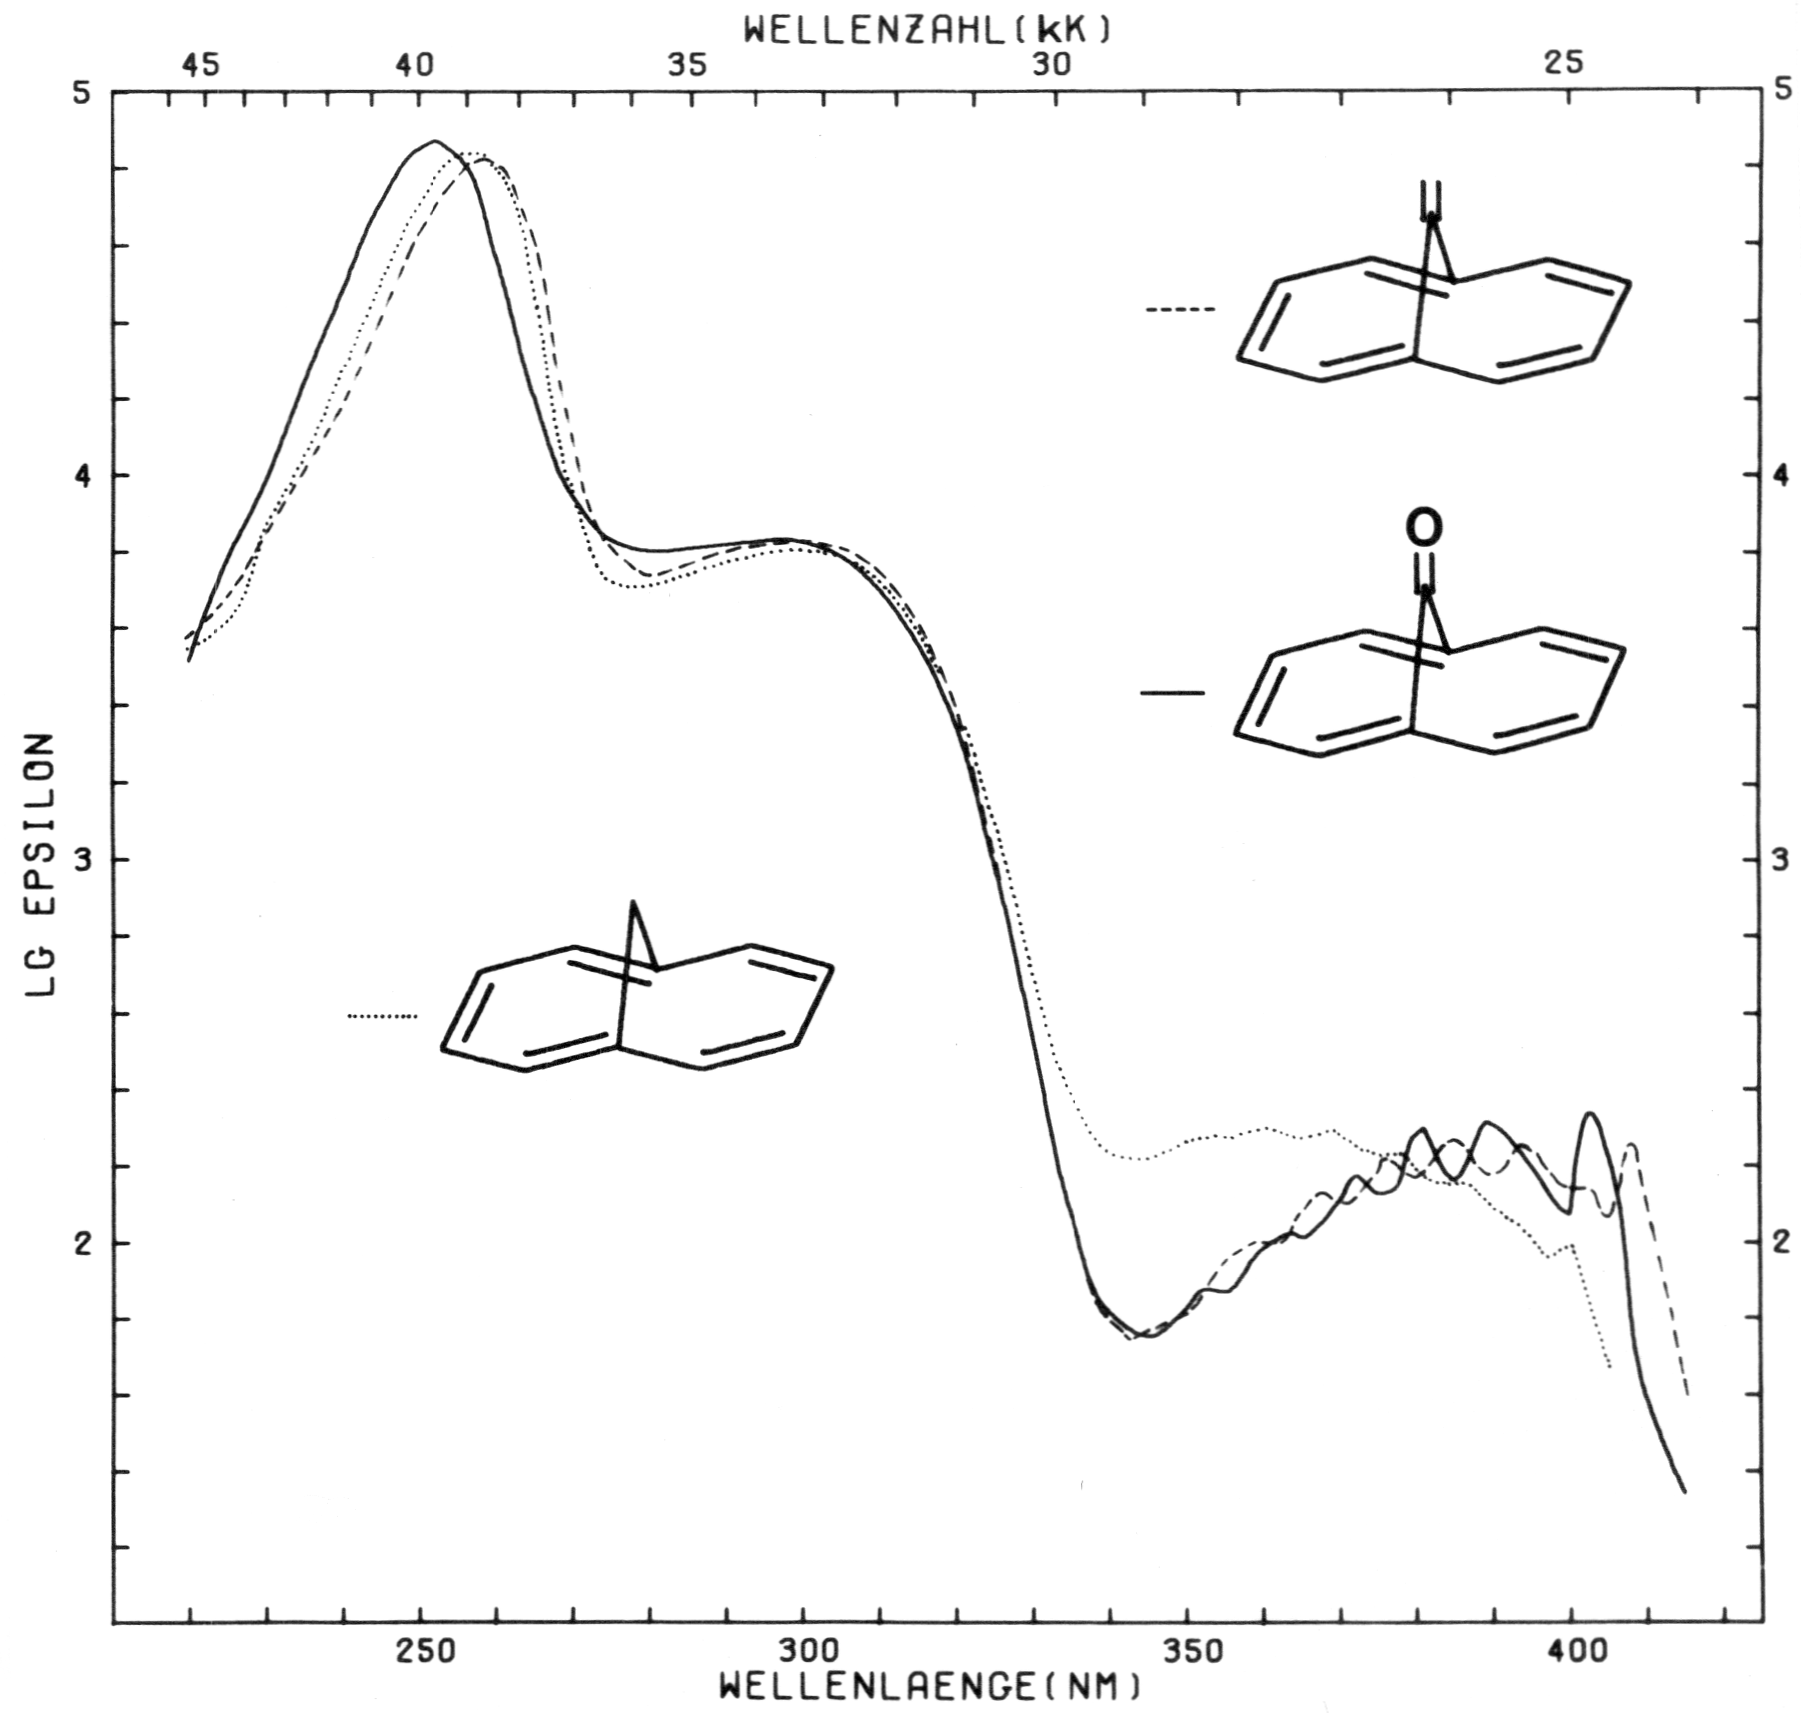
\includegraphics[width=15.25cm]{UV_015}
\begin{alltt}
Abb. 15: UV-Spektren des 11-Oxo-1,6-methano-[10]annulens (15), des
         11-Methylen-1‚6-methano-[10]annulens (17) in Cyclohexan
         und des 1,6-Methano-[10]annulens (16) in Dioxan

lassen allerdings auf eine höhere Delokalisation der \(\pi\)-Elektronen
über den Perimeter schließen. Wegen der großen Ähnlichkeit der
UV-Spektren aller drei angesprochenen Verbindungen kann eine signi-
fikante Wechselwirkung zwischen Carbonylgruppe und \(\pi\)-Elektronen-
system im Keton (15) mit Sicherheit ausgeschlossen werden.

\newpage
\makebox[0.8\textwidth][c]{- 36 -}


2.1.4.4 Schlußbetrachtung

Alle im Vorhergehenden aus den Spektren des Ketons (15) gewonnenen
Aussagen werden eindrucksvoll durch die Röntgenstrukturanalyse
untermauert. Nach Untersuchungen von S. Ito und Y. Fukazawa \raise0.5ex\hbox{[96]}
sind die Bindungslängen in etwa genauso angeglichen wie im Fall
der 1,6-Methano-[10]annulen-2-carbonsäure (43) \raise0.5ex\hbox{[97]} und des
11‚11-Difluor-1,6-methano-[10]annulens (44) \raise0.5ex\hbox{[98]} (vgl. Tab. 3).

\end{alltt}
% allow numbering of atoms, first=number, second=angle
\def\atom#1#2{-[:#2,0.3,,,draw=none]{\scriptstyle#1}}
\begin{table}[h!]\ttfamily
\captionsetup{singlelinecheck = false, justification=justified, labelfont=tt, textfont=tt}
\caption[caption]
    {\tabular[t]{@{}l@{}}Röntgenographische Daten der 1,6-Methano-[10]annulen-2-\\
    carbonsäure (43), des 11‚11-Difluor-1‚6-methano-[10]annu-\\
    lens (44) und des 11-Oxo-1,6-methano-[10]annulens (15)\\
    (Bindungslängen in {\AA}; Winkel in Grad)\endtabular}
\label{tab:RoentgenDaten}
\begin{varwidth}{\columnwidth}
 \hspace{2cm}
 \begin{tabular}{cp{1cm}c}
\schemestart
% kleiner Kreis
\def\emptydisk{\tikz\draw[thick](0,0)circle(2pt);}
 % [10]Annulenperimeter von oben
\definesubmol\nobondo{-[:66,0.3,,,draw=none]}
\definesubmol\nobondu{-[:-66,0.4,,,draw=none]}
\definesubmol\nobondh{-[:132,0.4,,,draw=none]}
% set scale and atom bond distance
\chemfig[atom style={scale=1.2},bond offset=0pt]{[,,,,,thick]%
-[:-36]\emptydisk%
-[:24]\emptydisk(-[:-66,0.4,,,draw=none]\scriptstyle6)%
(-[:111,0.8]?\emptydisk(-[:132,0.4,,,draw=none]\scriptstyle11)%
(-[:-6,0.5,,,draw=none]{\scriptstyle\alpha}))%
-[@{n1,-0.1}:-24]\emptydisk(-[:-45,0.4,,,draw=none]\scriptstyle5)% 5
-[:36]\emptydisk(-[:-15,0.4,,,draw=none]\scriptstyle4)%
-[:90]\emptydisk(-[:0,0.4,,,draw=none]\scriptstyle3)%
-[:144]\emptydisk(-[:45,0.3,,,draw=none]\scriptstyle2)%
-[@{n2,1.1}:-156]?\emptydisk(!\nobondo\scriptstyle1)%
-[:156]\emptydisk%
-[:-144]\emptydisk%
-[:-90]\emptydisk}%
\chemmove[>=Stealth]{\draw[<->,shorten <=2pt,shorten >=2pt](n1)..controls +(30:6mm) and +(-30:6mm)..(n2);}
\schemestop
 &   & %
\begingroup
% kleiner Kreis
\def\emptydisk{\tikz\draw[thick](0,0)circle(2pt);}
% set scale and atom bond distance
\chemfig[atom style={scale=1.2},bond offset=0pt]{[,,,,,thick]%
\emptydisk-[:9]\emptydisk-[:24]\emptydisk(-[:-90,0.4,,,draw=none]\scriptstyle1,6)%
(-[:45,0.3,,,draw=none]{\scriptstyle\beta})%
(-[@{n1,0.6}:90]\emptydisk(-[:90,0.3,,,draw=none]\scriptstyle11))% 11
-[@{ce}:-24]\emptydisk(-[:-90,0.4,,,draw=none]\scriptstyle2,5)% 2,5
(-[:45,0.3,,,draw=none]{\scriptstyle\gamma})%
-[@{n2}:-9]\emptydisk(-[:-90,0.4,,,draw=none]\scriptstyle3,4)
}% 
\chemmove[>=Stealth]{\draw[<-,shorten <=1pt,shorten >=1pt](n1)..controls +(6:6mm) and +(60:6mm)..(ce);}
\chemmove[>=Stealth]{\draw[->,shorten <=1pt,shorten >=1pt](n2)..controls +(81:6mm) and +(60:6mm)..(ce);}
\endgroup
\end{tabular}
 \\[18pt]
\hspace*{-0.75cm} 
 \begin{tabular}{cccccllccc}
 \  & \  & C1-C2 & C2-C3 & C3-C4 & C1-C6 & \quad\(\alpha\) & \(\beta\) & \(\gamma\) & Liter.\\
% 1,6-Methano-[10]annulen-2-carbonsäure (43)
\chemfig[atom style={scale=0.8}]{=_[:60,,,,shrtdbl={0pt}{3.5pt}]-[:12]=_[:-12]%
(-[:-252]?)% 1,6 Bruecke
-[:12](-[:60]CO_2H)=_[:-12,,,,shrtdbl={4pt}{0pt}]-[:-120]=_[:-168]-[:168]?=_[:-168,,,,shrtdbl={1pt}{2pt}]-[:168]}%
\cmpd*{methano10annulen2saeure}%
 & (43) & 1.40 & 1.38 & 1.41 & 2.257 & \ 99.6 & 108 & 162 & [97]\\[18pt]
% 11,11-Difluor-1,6-Methano-[10]annulen (44)
\chemfig[atom style={scale=0.8}]{=_[:60,,,,shrtdbl={0pt}{3.5pt}]-[:12]=_[:-12]%
(-[:-252]?(-[:165]F)(-[:15]F))% 1,6 Bruecke
-[:12]=_[:-12,,,,shrtdbl={4pt}{0pt}]-[:-120]=_[:-168]-[:168]?=_[:-168,,,,shrtdbl={1pt}{2pt}]-[:168]}%
\cmpd*{difluormethyano10annulen}%
 & (44) & 1.42 & 1.41 & 1.39 & 2.22 & 101\ \  & \  & \  & [98]\\[18pt]
% 11-Oxo-1,6-Methano-[10]annulen (15)
\chemfig[atom style={scale=0.8}]{=_[:60,,,,shrtdbl={0pt}{3.5pt}]-[:12]=_[:-12]%
(-[:-252]?(=[:90,0.6]O))% 1,6 Bruecke
-[:12]=_[:-12,,,,shrtdbl={4pt}{0pt}]-[:-120]=_[:-168]-[:168]?=_[:-168,,,,shrtdbl={1pt}{2pt}]-[:168]}%
\cmpd*{hexaentroponophan}%
 & (15) & 1.42 & 1.38 & 1.39 & 2.348 & 106.1 & 107 & 167 & [96]\\[18pt]
 \end{tabular}
 \end{varwidth}
\end{table}

\begin{alltt}
Die Diederwinkel im Perimeter von (15) sind so beschaffen, daß das
Kohlenstoffgerüst wesentlich flacher ist und geringer abgebeugt
erscheint als in den beiden anderen [10]Annulenen, was eine höhere
Delokalisation der \(\pi\)-Elektronen zur Folge hat. In dieser Tatsache
manifestiert sich der große Winkel C1-C11-C6, der den Abstand C1-C6
auf 2.348 {\AA} aufweitet. Zugleich jedoch ist dieser Winkel mit 106.1\degree
kleiner als in normalen Carbonylverbindungen und nur vergleichbar
mit den Werten in Fünfringketonen. Anhand dieser Daten dürfte eine
Valenztautomerie Bis-cycloheptatrien \(\rightleftarrows\) Bis-norcaradien, wie sie

\newpage
\makebox[0.8\textwidth][c]{- 37 -}


kürzlich für verschiedene [10]Annulene nachgewiesen wurde \raise0.5ex\hbox{[88]},
auszuschließen sein. Außerdem verneint die Röntgenstrukturanalyse
ausdrücklich eine Konjugation der Carbonylgruppe mit dem delokali-
sierten Elektronendezett, da die Kohlenstoff-Sauerstoff-Distanz
mit 1.221 {\AA} durchaus mit den Werten Für isolierte Ketone in Ein-
klang steht. Auch die Bindungen C1-C11 bzw. C6-C11 sind mit durch-
schnittlich 1.47 {\AA} typisch für die Länge einer Kohlenstoff-Einfach-
bindung in einem unkonjugierten C=C-C=O - System \raise0.5ex\hbox{[99]}.


2.1.5 Chemische Reaktionen des 11-Oxo-1‚6-methano-[101annulens (15)

Bei allen bisher unternommenen Reaktionen fällt die große Bereit-
schaft des Ketons (15) ins Auge, unter Kohlenmonoxidabspaltung in
Naphthalin (21) überzugehen, da hierdurch der anscheinend für eine
sp\raise0.5ex\hbox{2}-Hybridisierung ungünstige Bindungswinkel C1-C11-C6 beseitigt
wird. Weiterhin ist infolge der höheren Einebnung des Annulenteils
die Naphthalinstruktur bereits vorgebildet.

Die für Ketone spezifischen Reaktionen, wie Umsetzung mit 2,5-
Dinitrophenylhydrazin, mit p-Toluolsulfonylhydrazid oder Ketali-
sierung mit Orthoameisensäureester, die ansonsten unter Protonen-
katalyse stabile Derivate ergeben, führen unweigerlich zu Naphtha-
lin (21) und geringen Mengen nicht identifizierter Nebenprodukte.
In diesem Zusammenhang sei nochmals auf die vergeblichen Oxida-
tionsversuche des 11-Hydroxy-1,6-methano-[10]annulens (20) hinge-
wiesen (s. S. 21 f.).

Versuche, eine elektrophile Substitution im Perimeter herbeizufüh-
ren, hatten ähnlich negative Ergebnisse: Entweder verhält sich das
Keton (15) völlig inert, oder es entstehen neben wechselnden Mengen
Edukt (15) substituierte Naphthalinderivate (z.B. bei der Einwir-
kung von elementarem Brom \raise0.5ex\hbox{[100]}. Einzig die Umsetzung des Annu-
lenons (15) mit N-Bromsuccinimid in Nitromethan scheint ein Reak-
tionsprodukt mit unversehrter Annulenstruktur zu geben, dessen
nähere Untersuchung jedoch noch aussteht.

\newpage
\makebox[0.8\textwidth][c]{- 38 -}

2.2 11-Oxobicyclo[4.4.1]undecatetraen-(1‚3,5,8) (14)


Die erfolgreiche Synthese des 11-Oxo-1,6-methano-[10]annulens (15)
macht auch die Existenz der ähnlich strukturierten Verbindungen
(13) und (14] wahrscheinlich.

\end{alltt}
\hspace{2.5cm}
% 11-Oxo-1,6-Methano-undecatrien (13)
\chemname{
\chemfig{=_[:60]-[:12]=_[:-12]
(-[:-252]?(=[:90,0.6]O))% 1,6 Bruecke
-[:12]-[:-12]-[:-120]-[:-168]-[:168]?=_[:-168]-[:168]}
}{\cmpd{trientroponophan}}
\hspace{1.0cm}
% 11-Oxo-1,6-Methano-undecatetraen (14)
\chemname{
\chemfig{=_[:60]-[:12]=_[:-12]
(-[:-252]?(=[:90,0.6]O))% 1,6 Bruecke
-[:12]-[:-12]=_[:-120]-[:-168]-[:168]?=_[:-168]-[:168]}
}{\cmpd{tetraentroponophan}}
\chemnameinit{}
\begin{alltt}

Es lag daher nahe, die Präparierung dieser [4](2,7)-Troponophane
in Angriff zu nehmen, und die Eigenschaften der neuen Verbindungen
im Kontrast zur aromatischen Referenzverbindung (15), aus der sie
durch sukzessive Entfernung der Doppelbindungen aus einer Ring-
hälfte entstehen, zu studieren.

\end{alltt}
\schemestart
\hspace{0.5cm}
% 11-Brom-1,6-methano-undecatetraen
\chemname{
\chemfig{=_[:60]-[:12]=_[:-12]%
(-[:-252]?(-[:15]Br))% 1,6 Bruecke
-[:12]-[:-12]=_[:-120]-[:-168]-[:168]?=_[:-168]-[:168]}%
}{\cmpd{brombicyclo11tetraen}}%
\arrow(.mid east--){->[\parbox[b]{2cm}{\textsf{1.\,AgOAc, 2.\,Hydrolyse}}]}[,1.5]
\mbox{~}%
\arrow(--.mid west){->[\raise1.5pt\hbox{\textsf{3.\,DMSO}}]}[,1.1]
% 11-Oxo-1,6-Methano-undecatetraen
\chemname{
\chemfig{=_[:60]-[:12]=_[:-12]%
(-[:-252]?(=[:90,0.6]O))% 1,6 Bruecke
-[:12]-[:-12]=_[:-120]-[:-168]-[:168]?=_[:-168]-[:168]}%
}{\cmpd{tetraentroponophan}}%
\schemestop
\chemnameinit{}
\begin{alltt}

Zur Darstellung der Titelverbindung eignet sich ein analoger Syn-
theseweg, wie er zum aromatischen Keton (15) führte.


2.2.1 11-\underline{endo}-Brombicyclo[4.4.l]undecatetraen-(1‚3,5,8) (45) \leavevmode\raise0.5ex\hbox{*})

Die Gewinnung des \underline{endo}-Bromids (45) bietet keine Schwierigkeiten,
tritt es doch bei der Dehydrierung des 11-Bromtricyclo[4.4.1.0\raise0.5ex\hbox{1.6}]-
undecadiens-(3,8) (24) zum 11-Brom-1,6-methano-[10]annulen (25) als
Nebenprodukt auf. Beim Umkristallisieren des Reaktionsproduktes

\(\overline{\hspace{7cm}}\)
\leavevmode\raise0.5ex\hbox{*}) Die Bezeichnungen \underline{endo}- bzw. \underline{exo}- in dieser Arbeit sind willkür-
   lich gewählt; \underline{endo}- bezeichnet immer den Substituenten, der sich
   über der Ringhälfte mit der geringeren Anzahl an Doppelbindungen
   befindet.

 

 

\newpage
\makebox[0.8\textwidth][c]{- 39 -}


\end{alltt}
\schemestart
\hspace{1.0cm}
% Bromtricycloundecadien (24)
\chemname{
\chemfig{=_[:60]-[:12]-[:-12]
(-[:-120]) % Einfachbindung 1 - 6
(-[:-252]?(-[:15]Br))% 1,6 Bruecke
-[:12]-[:-12]=_[@{ab,0.3}:-120]-[:-168]-[:168]?-[:-168]-[:168]}
}{\cmpd{bromtricyclo11dien}}
\arrow(@ab--[xshift=-6pt]){->[\chemfig{DDCh}]}[,1.0]
\mbox{~}
\arrow(mb--.mid west){->}[45]% node at mbox
% 11-Brom-1,6-methano-[10]annulen (25)
\chemname{
\chemfig{=_[:60]-[:12]=_[:-12]
(-[:-252]?(-[:15]Br))% 1,6 Bruecke
-[:12]=_[:-12]-[:-120]=_[:-168]-[:168]?=_[:-168]-[:168]}
}{\cmpd{bromomethano10annulen}}
\arrow(@mb--.mid west){->}[-45]
% 11-Brom-1,6-methano-undecatetraen (45)
\chemname{
\chemfig{=_[:60]-[:12]=_[:-12]
(-[:-252]?(-[:15]Br))% 1,6 Bruecke
-[:12]-[:-12]=_[:-120]-[:-168]-[:168]?=_[:-168]-[:168]}
}{\cmpd{brombicyclo11tetraen}}
\schemestop
\chemnameinit{}
\begin{alltt}

verbleibt des \underline{endo}-Bromid (45) in der Mutterlauge und kann bis auf
etwa 50 \% angereichert Werden. Eine Reindarstellung des 11-\underline{endo}-
Brombicyclo[4.4.1]undecatetraens-(1‚3,5,8) (45) gelingt durch
mehrtägige Säulenchromatographie des 50:50 Gemisches an Aluminium-
oxid (Eluens: Pentan), wobei das Bromid (45) in Form weißer Nadeln
vom Fp = 49 - 51\degree{}C anfällt. Aus einem Ansatz von 0.1 Mol 11-Brom-
tricyclo[4.4.1.0\raise0.5ex\hbox{1,6}]undecadien-(3,8) (24) erhält man so neben
19.4 g aromatischem Bromid (25) noch 1.3 g \underline{endo}-Bromid (45), das
allerdings auch auf unabhängigem Wege synthetisiert wurde \raise0.5ex\hbox{[42]}.
Da das 11-Brom-1,6-methano-[10]annulen (25) jedoch in relativ
großen Mengen benötigt wurde, konnten die für die Synthese des
Ketons (14) erforderlichen Quantitäten \underline{endo}-Bromid (45) bequem
dargestellt werden.

\end{alltt}
\schemestart
% für korrekte Bezifferung vorab definieren
\cmpd*{acetoxybicyclo11tetraen}% (46)
\cmpd*{hydroxybicyclo11tetraen}% (47)
% Dibromcarbenaddukt (23)
\chemname{
\chemfig{=_[:60]-[:12]-[:-12]%
(-[:-120])% Einfachbindung 1 - 6
(-[:-252]?(-[:165]Br)(-[:15]Br))% 1,6 Bruecke
-[:12]-[:-12]=_[:-120]-[:-168]-[:168]?-[:-168]-[:168]}%
}{\cmpd{dibromcarbenaddukt}}
\arrow(.east--.west){->[\chemfig{DDCh}]}[,1.2]
% Dibromtricycloundecadien (48)
\chemname{
\chemfig{=_[:60]-[:12]=_[:-12]
(-[:-252]?(-[:165]Br)(-[:15]Br))% 1,6 Bruecke
-[:12]-[:-12]=_[:-120]-[:-168]-[:168]?=_[:-168]-[:168]}
}{\cmpd{dibrombicyclo11tetraen}}
\arrow(.east--.west){->[\chemfig{{-}Br}]}[,1.0]
% 11-Brom-1,6-methano-undecatetraen (45)
\chemname{
\chemfig{=_[:60]-[:12]=_[:-12]
(-[:-252]?(-[:15]Br))% 1,6 Bruecke
-[:12]-[:-12]=_[:-120]-[:-168]-[:168]?=_[:-168]-[:168]}
}{\cmpd{brombicyclo11tetraen}}
\schemestop
\chemnameinit{}
\begin{alltt}

Eine rationelle Synthese würde vom 11‚11-Dibromtricyclo[4.4.1.0\raise0.5ex\hbox{1,6}]-
undecadien-(3,8) (23) ausgehen und sich die Tatsache zunutze machen,
daß 11‚11-dihalogensubstituierte Tricycloundecadiene bei der Behand-
lung mit DDQ nur in einer Ringhälfte dehydriert werden \raise0.5ex\hbox{[101]}. Die
weiteren Umsetzungen erfolgen nach konventionellen Methoden.


Im \raise0.5ex\hbox{1}H-NMR-Spektrum (s. Abb. 16 auf S. 40) gibt der Trienteil (H-2 -
H-5) Anlass zu einem AA'XX'-System mit \(\nu\)\lower0.5ex\hbox{A} = 3.22\(\tau\) und \(\nu\)\lower0.5ex\hbox{X} = 4.03\,\(\tau\).
Der N-Wert von 5.5 Hz ist mit der Cycloheptatrienstruktur in Ein-
klang \raise0.5ex\hbox{[102]}. Die beiden olefinischen Protonen H-8 und H-9 treten

\newpage
\makebox[0.8\textwidth][c]{- 40 -}    



\end{alltt}
\hspace*{-0.5cm}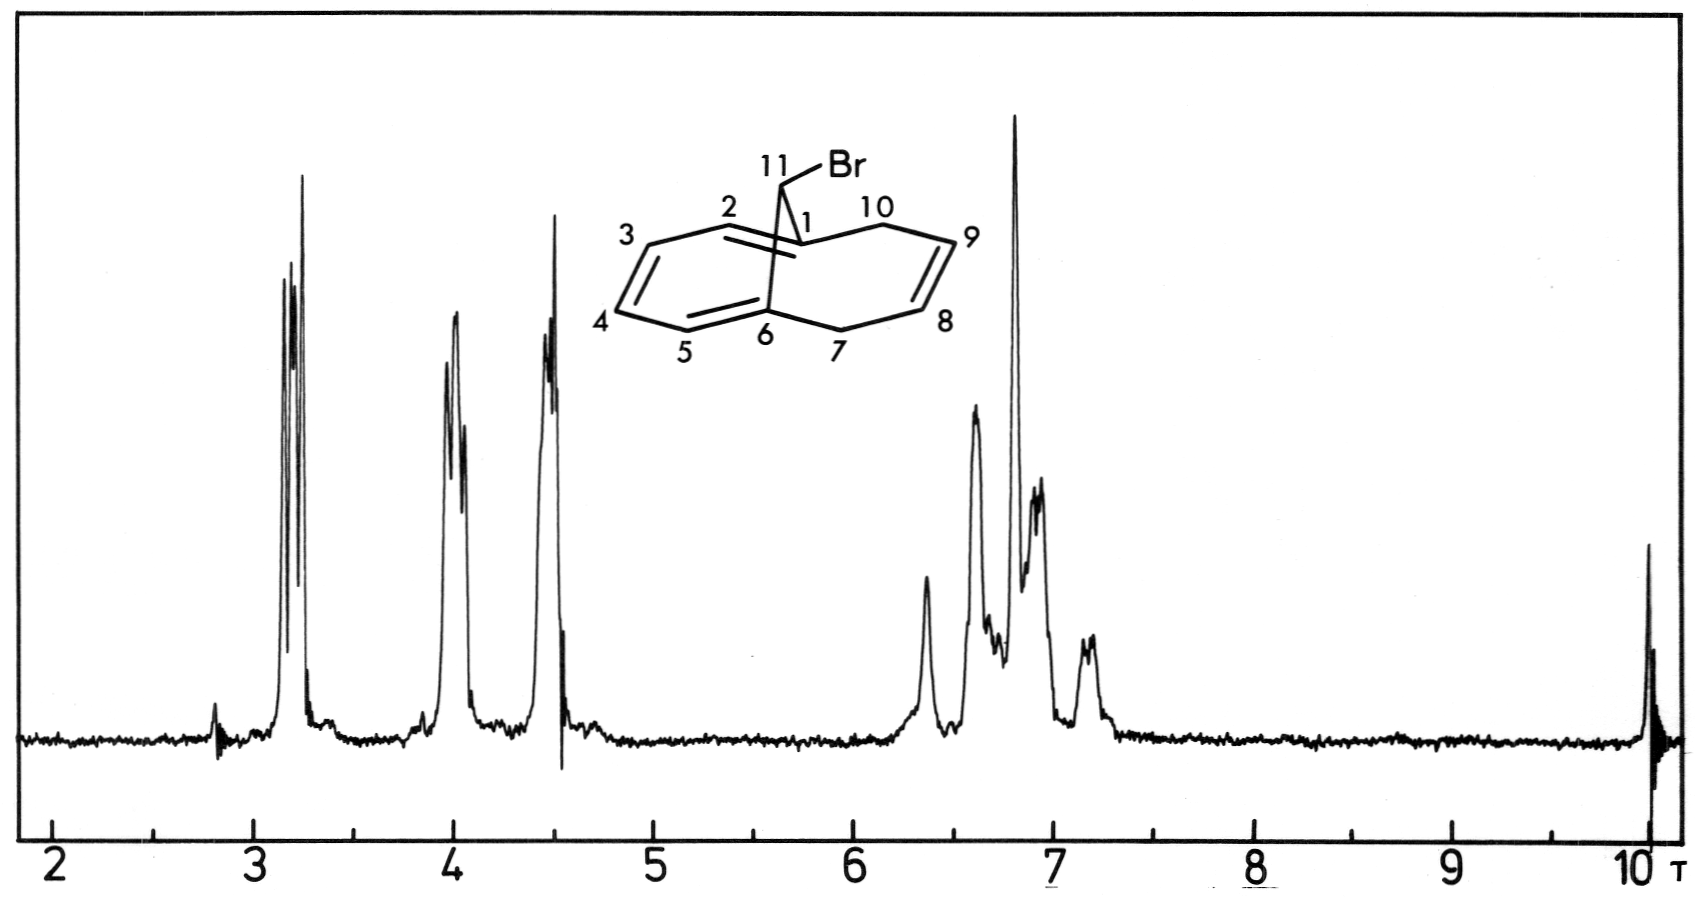
\includegraphics[width=14.35cm]{NMR_016}
\begin{alltt}
Abb. 16: \raise0.5ex\hbox{1}H-NMR-Spektrum des 11-\underline{endo}-Brombicyclo[4.4.ljundeca-
tetraens-(1,3‚5‚8) (45) in CDCl\lower0.5ex\hbox{3} (60 MHz; TMS als innerer
Standard)

 

bei \(\tau\) = 4.35 - 4.73 in Resonanz, während die allylischen Protonen
an C-7 bzw. C-10 bei \(\tau\) = 6.22 - 7.35 als Multiplett mit AB-Charak-
ter absorbieren (J\lower0.5ex\hbox{AB} = 14 Hz). Die \underline{endo}-Stellung des Substituenten
folgt aus der hohen Absorptionslage von H-11 bei \(\tau\) = 6.83, da das
Brückenproton oberhalb der \(\pi\)-Bindungen der dreifach ungesättigten
Ringhälfte eine Abschirmung erfährt, die den induktiven - entschir-
menden - Effekt des benachbarten Bromatoms teilweise kompensiert.


2.2.2 11-\underline{endo}-Acetoxybicyclo[4.4.1]undecatetraen-(l‚3,5,8) (46)

Eine Substitution des Bromatoms durch die Acetoxygruppe findet beim
Erhitzen des 11-\underline{endo}-Brombicyclo[4.4.1]undecatetraens-(1‚3,5,8)
(45) mit Silber(I)acetat in Eisessig statt. Diese drastischen
Bedingungen führen innerhalb 24 h zum vollständigen Umsatz des
Eduktes. Außer 11-\underline{endo}-Acetoxybicyclo[4.4.1]undecatetraen-(1‚3,5,8)
(46) werden keine weiteren Reaktionsprodukte beobachtet, so daß
solvolytische Umlagerungen auszuschließen sind. Überhaupt scheint

 

\newpage
\makebox[0.8\textwidth][c]{- 41 -}


das intermediär entstehende Carboniumion an C-11 von den übrigen
\(\pi\)-Systemen des Perimeters völlig isoliert zu sein, wie es auch
im entsprechenden 1,6-Methano-[10]annuleniumion der Fall ist \raise0.5ex\hbox{[42]}.
Weiterhin ist die \(\pi\)-Elektronendichte über dem Trienteil so groß,
daß eine Annäherung des Substituenten nur von der anderen Seite
erfolgen kann, weshalb trotz des wahrscheinlichen S\lower0.5ex\hbox{N1}-Mechanismus'
nur Retention beobachtet wird.

\end{alltt}
\schemestart
\hspace{1.25cm}
% 11-Brom-1,6-methano-undecatetraen (45)
\chemname{
\chemfig{=_[:60]-[:12]=_[:-12]
(-[:-252]?(-[:15]Br))% 1,6 Bruecke
-[:12]-[:-12]=_[:-120]-[:-168]-[:168]?=_[:-168]-[:168]}
}{\cmpd{brombicyclo11tetraen}}
\arrow(.mid east--.mid west){->[\chemfig{AgOAc}]}[,1.2]
% 11-Acetoxy1,6-methano-undecatetraen (46)
\chemname{
\chemfig{=_[:60]-[:12]=_[:-12]
(-[:-252]?(-[:15]OCOCH_3))% 1,6 Bruecke
-[:12]-[:-12]=_[:-120]-[:-168]-[:168]?=_[:-168]-[:168]}
}{\cmpd{acetoxybicyclo11tetraen}}
\schemestop
\chemnameinit{}
\begin{alltt}

Das 11-\underline{endo}-Acetoxybicyclo[4.4.1]undecatetraen-(1‚3,5,8) (46) wird
nach Verdünnen der Reaktionsmischung mit Wasser und Extraktion mit
Pentan in Form weißer Kristallnadeln isoliert, die nach Umkristal-
lisieren aus Petroläther einen konstanten Schmelzounkt von 86 -
87\degree{}C aufweisen.

Die angenommene Summenformel C13H14O2 wird durch die Elementarana-
lyse bestätigt. Die Anwesenheit einer Estergruppierung im Molekül

\end{alltt}
\hspace*{-0.25cm}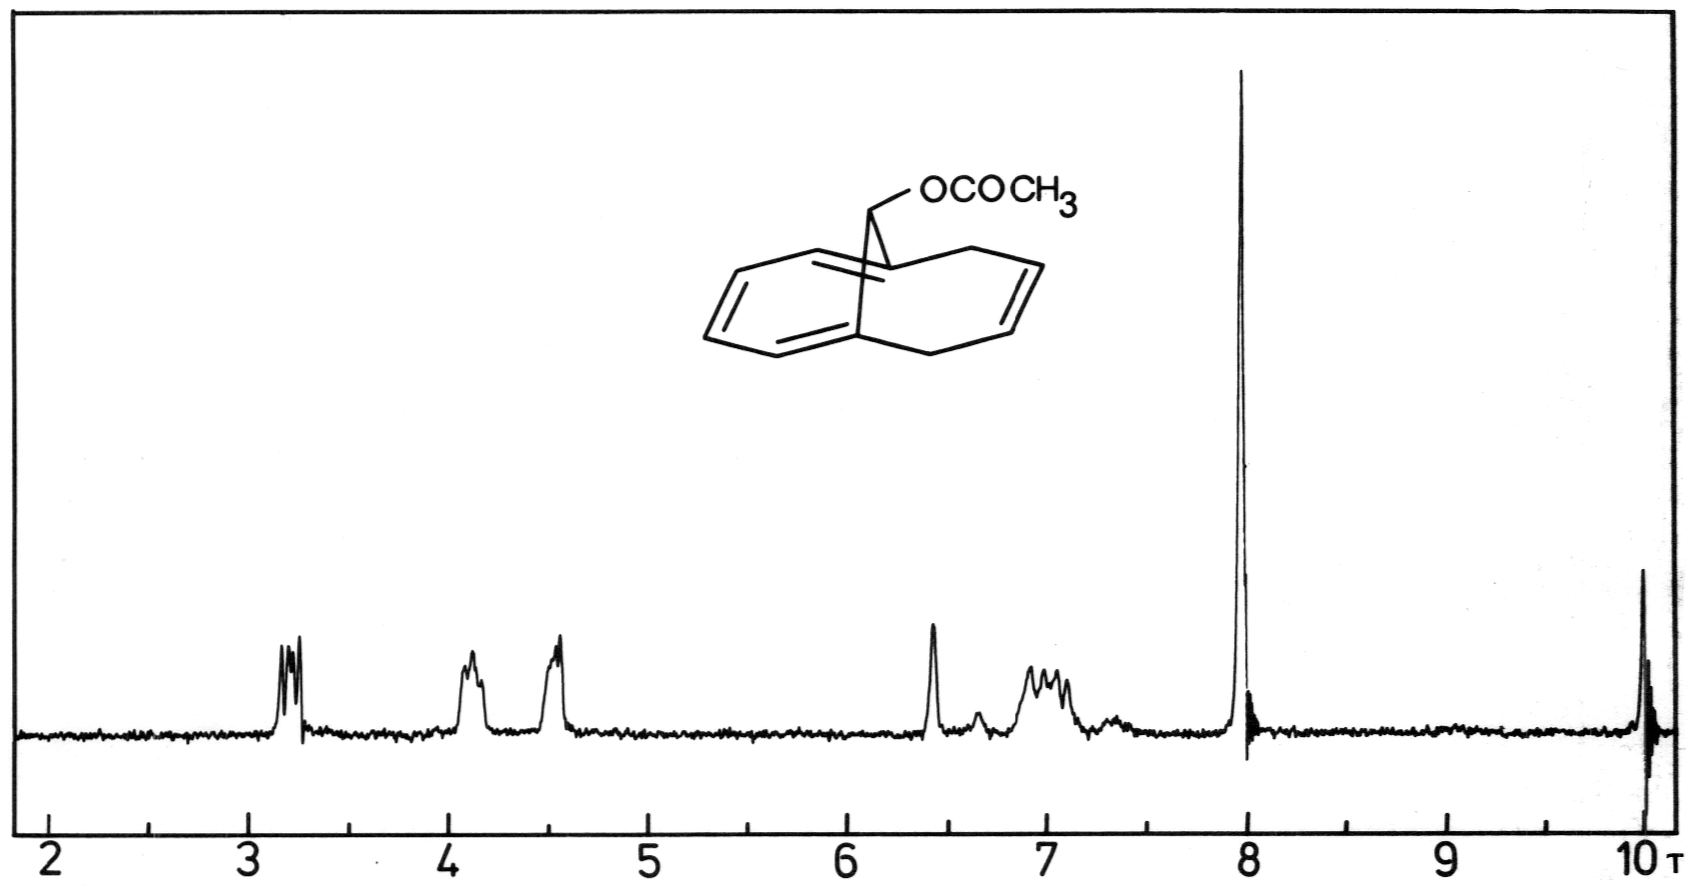
\includegraphics[width=14.29cm]{NMR_017}
\begin{alltt}
Abb. 17: \raise0.5ex\hbox{1}H-NMR-Spektrum des 11-\underline{endo}-Acetoxybicyclo[4.4.1]undeca-
tetraens-(1,3,5,8) (46) in CCl\lower0.5ex\hbox{4} (60 MHz; TMS als innerer
Standard)
\newpage
\makebox[0.8\textwidth][c]{- 42 -}


dokumentiert sich überzeugend im IR-Spektrum, das charakteristische
Banden hoher Intensität bei 1756 cm\raise0.5ex\hbox{-1} und 1742 cm\raise0.5ex\hbox{-1} (\(\nu\)\lower0.5ex\hbox{C=O}) sowie
bei 1240 cm\raise0.5ex\hbox{-1} und 1064 cm\raise0.5ex\hbox{-1} (\(\nu\)\lower0.5ex\hbox{C-O}) zeigt.

Laut \raise0.5ex\hbox{1}H-NMR-Spektrum (s. Abb. 17 auf S. 41) hat tatsächlich nur
ein Austausch des Brückensubstituenten stattgefunden, da die ole-
finischen Protonen gegenüber dem Bromderivat (45) an fast identi-
schen Stellen absorbieren. Vier Protonen (H-2 - H-5) bilden ein
AA'XX'-System mit \(\nu\)\lower0.5ex\hbox{A} = 3.23\(\tau\) und \(\nu\)\lower0.5ex\hbox{X} = 4.15\(\tau\) (N = 5.5 Hz), während
die Protonen der isolierten Doppelbindung bei \(\tau\) = 4.43 - 4.68 er-
scheinen. Bedingt durch die Acetatgruppe wird das Brückenproton
um 0.4 ppm nach tieferem Feld verschoben (\(\tau\) = 6.45), und das
Multiplett für die allylischen Protonen bei \(\tau\) = 6.57 - 7.45 rückt
enger zusammen. Die Methylprotonen des Acetatrestes geben ein
Singulett bei \(\tau\) = 7.99.

Auch das Elektronenspektrum spricht mit einem Maximum bei 252 nm
(\(\epsilon\) = 4400) für ein intaktes Doppelbindungssystem.

 
2.2.3 11-\underline{endo}-Hydroxybicyclo[4.4.1]undecatetraen-(1‚3,5,8) (47)

 Zur Spaltung des Acetates (46) wird wie beim entsprechenden
1‚6-Methano-[10]annulenderivat (35) Methylmagnesiumjodid in Äther
eingesetzt. Nach Zugabe des Eduktes (46) in fester Form zur
GRIGNARD-Verbindung setzt die Umsetzung - erkenntlich am Ausfallen
von Magnesiumsalzen - nach kurzer Induktionsperiode ein. Die üb-
liche wässrig-extraktive Aufarbeitung nach etwa 2 h Reaktionszeit
liefert in fast quantitativer Ausbeute weiße Kristalle, die nach
Umlösen aus Äther/Hexan als farblose Quader vom Fp = 126 - 127\degree{}C
vorliegen.

\end{alltt}
\schemestart
\hspace{1.25cm}
% 11-Acetoxy1,6-methano-undecatetraen (46)
\chemname{
\chemfig{=_[:60]-[:12]=_[:-12]
(-[:-252]?(-[:15]OCOCH_3))% 1,6 Bruecke
-[:12]-[:-12]=_[:-120]-[:-168]-[:168]?=_[:-168]-[:168]}
}{\cmpd{acetoxybicyclo11tetraen}}
\arrow(.mid east--.mid west[xshift=5mm]){->[\chemfig{MeMgJ}]}[,1.2]
% 11-Hydoxy1,6-methano-undecatetraen (47)
\chemname{
\chemfig{=_[:60]-[:12]=_[:-12]
(-[:-252]?(-[:15]OH))% 1,6 Bruecke
-[:12]-[:-12]=_[:-120]-[:-168]-[:168]?=_[:-168]-[:168]}
}{\cmpd{hydroxybicyclo11tetraen}}
\schemestop
\chemnameinit{}
\begin{alltt}

\newpage
\makebox[0.8\textwidth][c]{- 43 -}

Alle spektroskopischen Daten sowie die korrekte Elementaranalyse
sprechen für einen Reaktionsablauf nach dem formulierten Schema.
So weist die breite Valenzschwingung der assoziierten Hydroxyle
bei 3390 cm\raise0.5ex\hbox{-1} im IR-Spektrum das neue Molekül als Alkohol aus.

             

\end{alltt}
\hspace*{-0.5cm}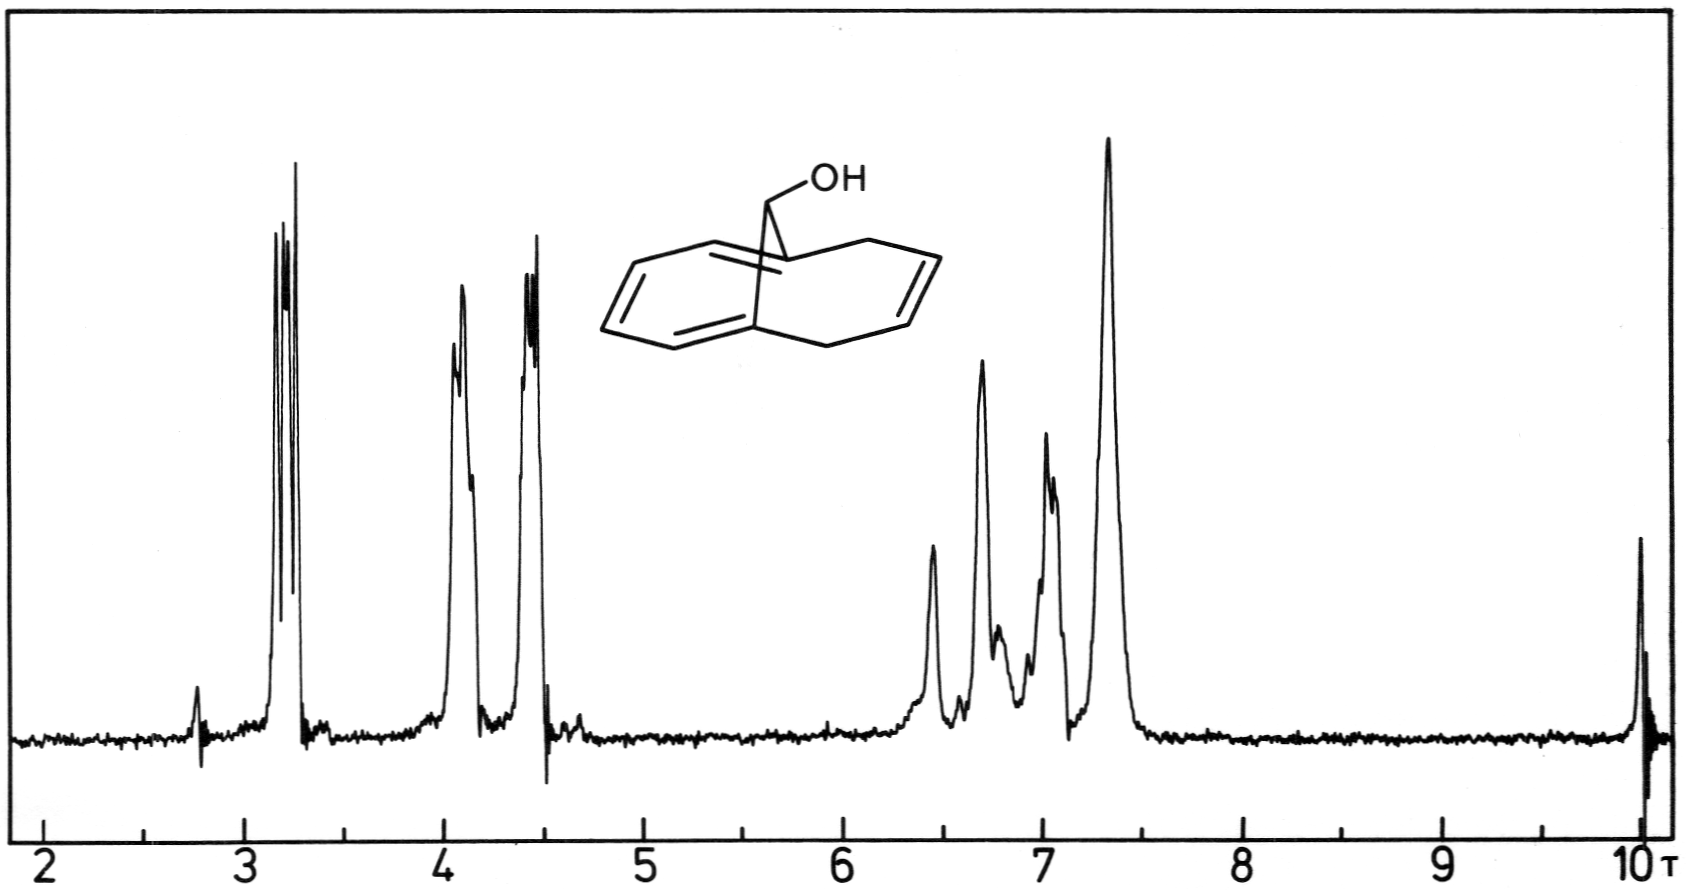
\includegraphics[width=14.31cm]{NMR_018}
\begin{alltt}
Abb. 18: \raise0.5ex\hbox{1}H-NMR-Spektrum des 11-\underline{endo}-Hydroxybicyclo[4.4.1]undeca-
tetraens-(1,3,5‚8] (47) in CDCl\lower0.5ex\hbox{3} (60 MHz; TMS als innerer
Standard)

 
Das \raise0.5ex\hbox{1}H-NMR-Spektrum lässt keinerlei Veränderung der Molekülstruktur
erkennen. Unverändert erscheinen das AA‘XX'-System für die Trien-
protonen bei \(\tau\) = 2.98 - 4.27 und das Multiplett für H-8 bzw. H-9
bei \(\tau\) = 4.27 - 4.72. Weiterhin beobachtet man bei \(\tau\) = 7.35 ein
breites Signal, das einer Überlagerung der Absorptionen für Hydro-
xyl- und Brückenproton entspricht, da man nach Zugabe von D2O nur
noch ein scharfes Singulett an dieser Stelle erhält. Die hohe
Resonanzfrequenz für das Proton H-11 stellt wiederum das stärkste
Argument für die Beibehaltung der \underline{endo}-Konfiguration des Substitu-
enten dar.

Das UV-Spektrum weist entsprechend der Cycloheptatrienstruktur nur
ein kurzwelliges Maximum bei 253 nm von geringer Extinktion
(\(\epsilon\) = 3800) auf.

\newpage
\makebox[0.8\textwidth][c]{- 44 -}

2.2.4 11-Oxobicyclo[4.4.1]undecatetraen-(1‚3,5,8) (14)

Die Oxidation des 11-\underline{endo}-Hydroxybicyclo[4.4.1]undecatetraens-
(1,3,5,8) (47) mit der neuen Kombination DMSO/Äthyl-[3-(dimethyl-
amino)propyl]carbodiimid-hydrochlorid/PTFA (s. S. 26) verläuft
problemlos. Das quantitativ anfallende Rohprodukt ergibt nach Um-
kristallisieren aus Äther/Hexan weiße Kristallnadeln, deren
Schmelzpunkt zu 94 - 95.5\degree{}C bestimmt wird.

\end{alltt}
\schemestart
\hspace{1.25cm}
% 11-Hydoxy1,6-methano-undecatetraen (47)
\chemname{
\chemfig{=_[:60]-[:12]=_[:-12]
(-[:-252]?(-[:15]OH))% 1,6 Bruecke
-[:12]-[:-12]=_[:-120]-[:-168]-[:168]?=_[:-168]-[:168]}
}{\cmpd{hydroxybicyclo11tetraen}}
\arrow(.mid east--.mid west){->[\chemfig{DMSO}]}[,1.2]
% 11-Oxo-1,6-Methano-undecatetraen (14)
\chemname{
\chemfig{=_[:60]-[:12]=_[:-12]
(-[:-252]?(=[:90,0.6]O))% 1,6 Bruecke
-[:12]-[:-12]=_[:-120]-[:-168]-[:168]?=_[:-168]-[:168]}
}{\cmpd{tetraentroponophan}}
\schemestop
\chemnameinit{}
\begin{alltt}

Neben der Elementaranalyse gibt schon das Massenspektrum einige
Hinweise zur Strukturaufklärung. Ähnlich dem Fragmentierungsmuster
des 11-Oxo-1‚6-methano-[10]annulens (15) ist der Molekülpeak bei
m/e = 158 sehr wenig ausgeprägt (rel. Int. 0.6 \%). Im Spektrum
dominiert das Signal bei m/e = 130 für das Dihydronaphthalin-
Radikalkation, das durch Kohlenmonoxidabspaltung aus dem Molekül-
ion entsteht. Sukzessiver Verlust von zwei Wasserstoffradikalen

 

\end{alltt}
\hspace*{-0.25cm}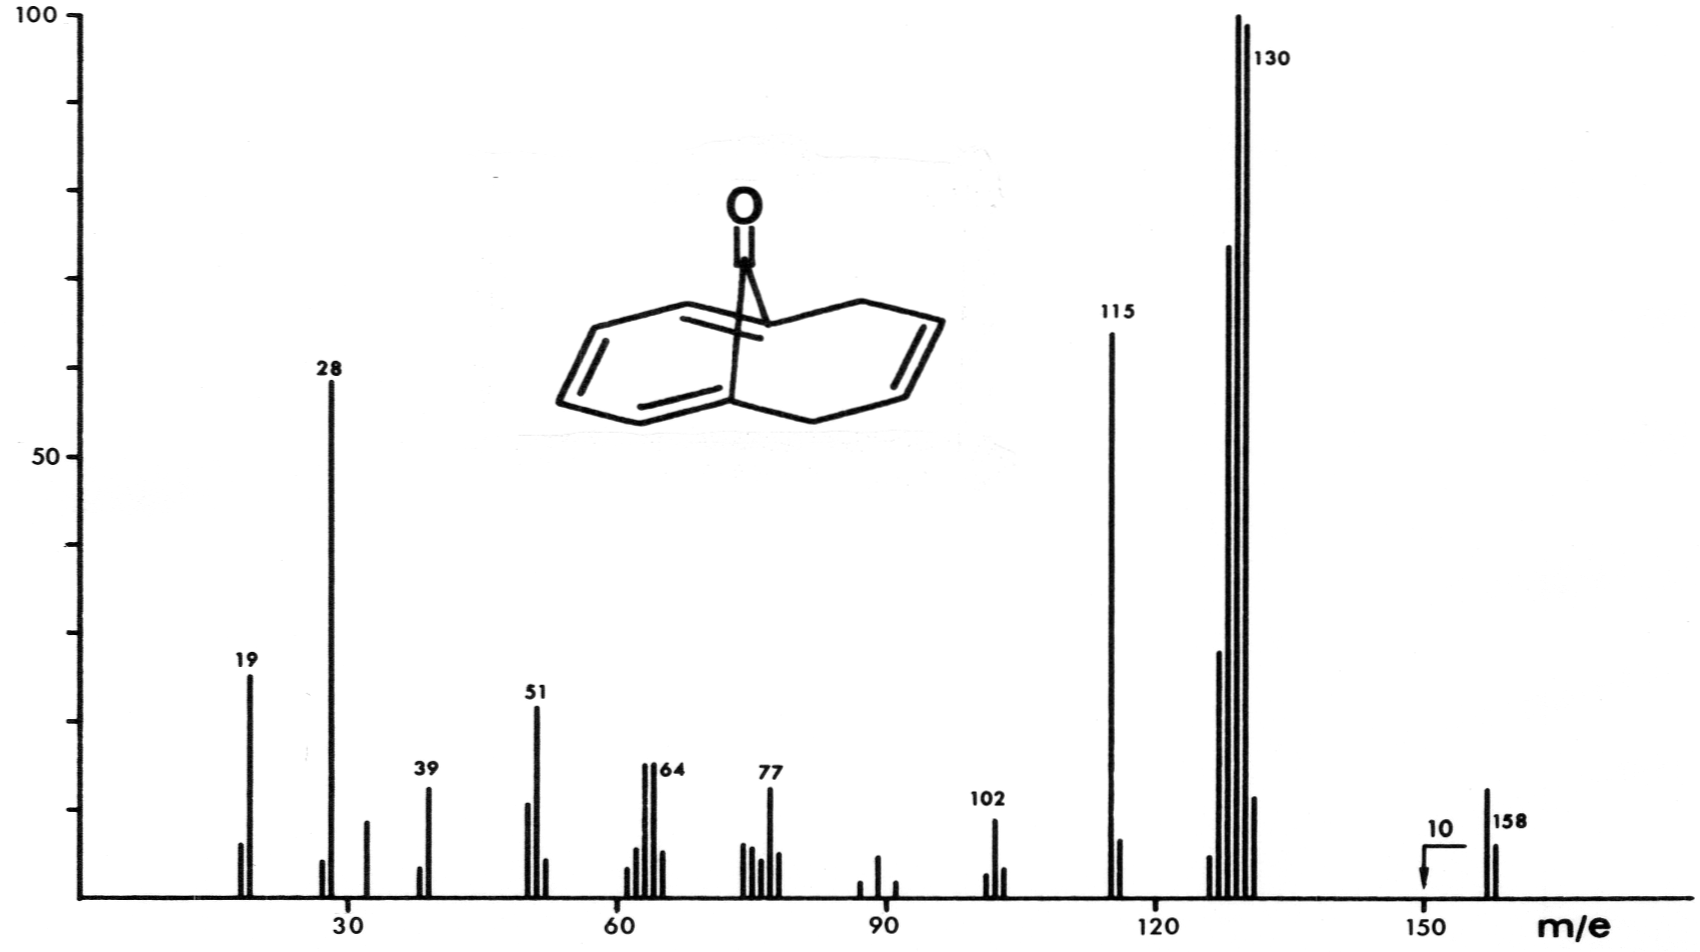
\includegraphics[width=14.39cm]{MASS_019}
\begin{alltt}
Abb. 19: Massenspektrum des 11-Oxobicyclo[4.4.1]undeoa-
tetraens-(1‚3,5‚8) (14) (100 eV)

\newpage
\makebox[0.8\textwidth][c]{- 45 -}

lässt Naphthalin entstehen, dessen weitere Zerfallsprodukte sich im
Spektrum wiederfinden lassen. Daneben existiert jedoch noch ein
weiterer Fragmentierungsgang, erkenntlich am Auftreten des Signals
bei m/e = 115 (64 \%], das dem Indenyliumkation entspricht. Diese
Spezies dürfte einer Ketenabspaltung aus einem Dihydrobenztropo-
niumion entstammen, das in einem vorgelagerten Reaktionsschritt
gemäß Schema 3 generiert wird.
\end{alltt}
\hspace*{0.5cm}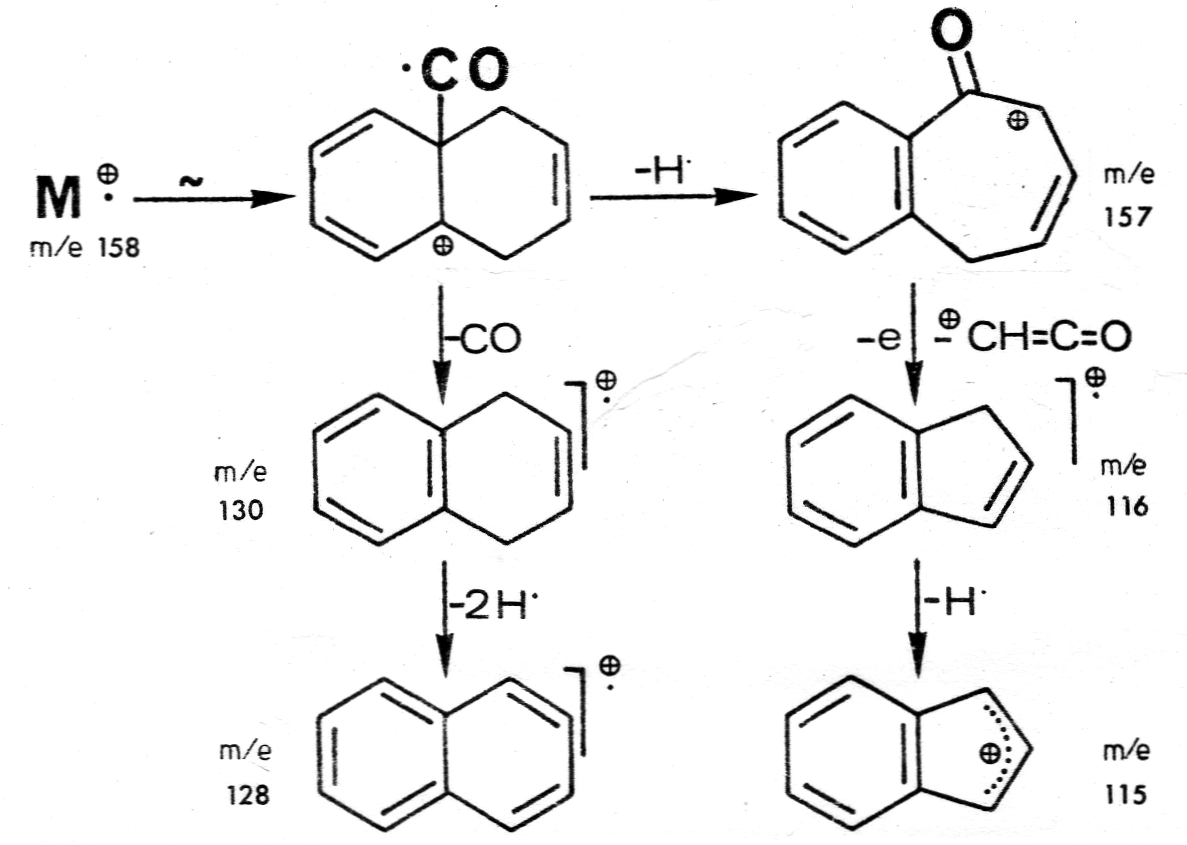
\includegraphics[width=10.05cm]{SCHEMA_003}
\begin{alltt}
Schema 3: Fragmentierungsverlauf des 11-Oxobicyclo[4.4.1]undeca-
tetraens-(1,3,5,8] (14) im Massenspektrum
 

Auch das IR-Spektrum lässt sich im Sinne von Struktur (14) inter-
pretieren: Die ausgeprägte Carbonyl-Valenzschwingung absorbiert
mit \(\nu\)\lower0.5ex\hbox{C=O} = 1740 cm\raise0.5ex\hbox{-1} im Vergleich zum aromatischen Keton (15) an
identischer Stelle, so daß auch ohne das Vorliegen einer Röntgen-
strukturanalyse für den Winkel C1-C11-C6 ein Wert von etwa 107\degree
postuliert werden kann.

Im \raise0.5ex\hbox{13}C-NMR-Spektrum (s. Abb. 20 auf S. 46) beobachtet man für die
Brückenbasisatome C-1 bzw. C-6 eine Resonanzfrequenz von "nur"
125.6 ppm, etwa 4 ppm niedriger als im aromatischen Keton (15).
Ob diese "hohe" Absorptionslage nur auf die Nachbarschaft der bei-
den sp\raise0.5ex\hbox{3}-hybridisierten Kohlenstoffatome C-7 und C-10, die bei \(\delta\) =
30.96 ppm in Resonanz treten, oder auf einen noch kleineren Dieder-
winkel C1-C11-C6 zurückzuführen ist, kann allerdings nicht ent-
schieden werden. Im Vergleich zum Annulenon (15) absorbiert der

\newpage
\makebox[0.8\textwidth][c]{- 46 -}


\end{alltt}
\hspace*{-0.25cm}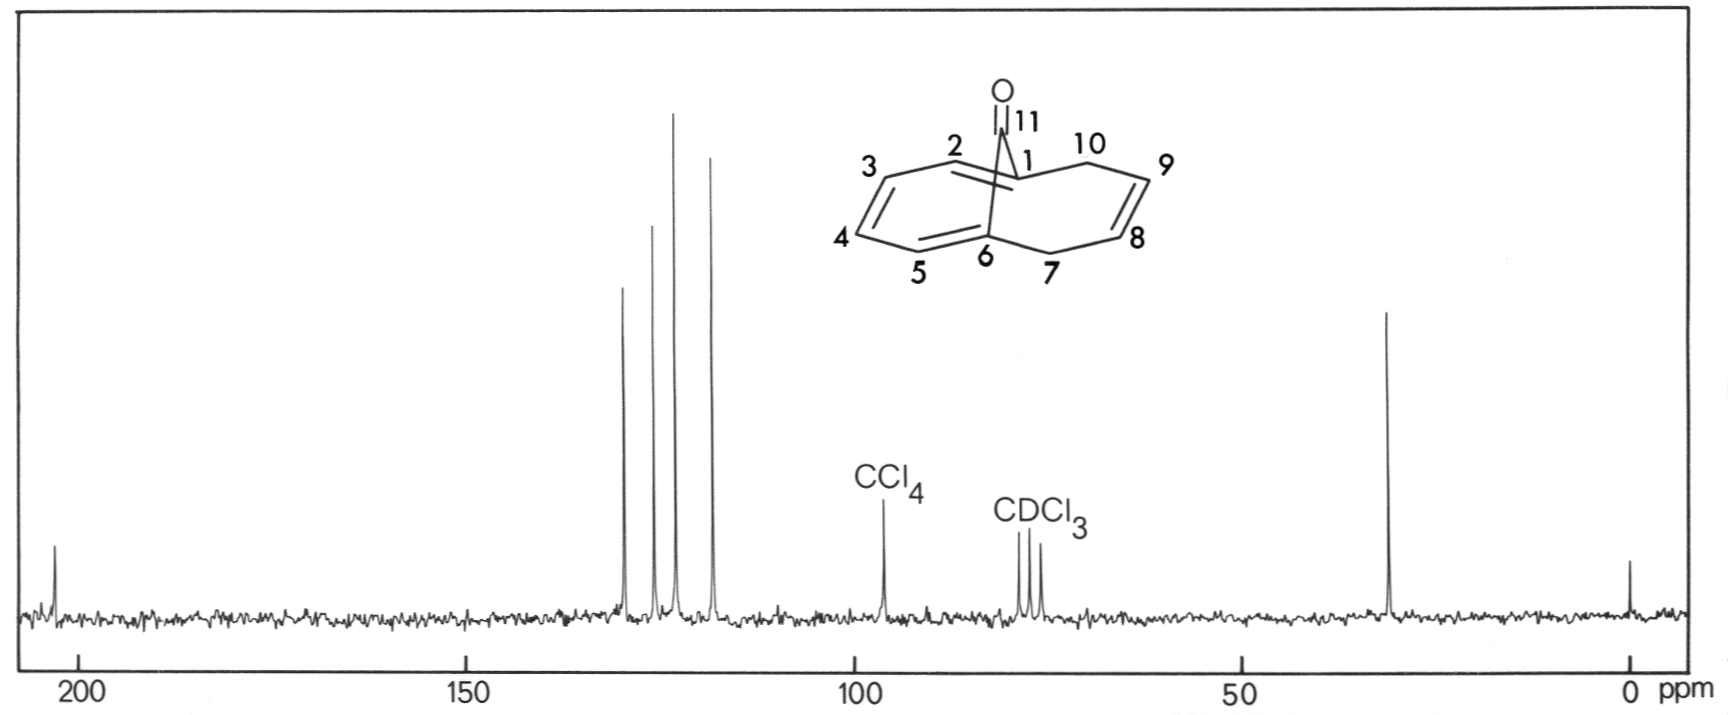
\includegraphics[width=14.63cm]{NMR_020}
\begin{alltt}
Abb. 20: \raise0.5ex\hbox{13}C-NMR-Spektrum des 11-Oxobicyclo[4.4.1]undecatetra-
ens-(1,3,5,8) (14) in CCl\lower0.5ex\hbox{4}/CDCl\lower0.5ex\hbox{3} 3:1 (-30\degree{}C; 22.63 MHz;
rauschentkoppelt; TMS als innerer Standard; Lockfrequenz:
\leavevmode\raise0.5ex\hbox{2}H-Resonanz des CDCl\lower0.5ex\hbox{3})

Carbonylkohlenstoff C-11 um 5.3 ppm höher bei \(\delta\) = 202.7 ppm, wäh-
rend die übrigen Signale in den für sp\raise0.5ex\hbox{2}-hybridisierte Kohlenstoffe
typischen Bereich fallen (C-3,4: \(\delta\) = 129.4 ppm; C-2,5: \(\delta\) = 117.9
ppm; C-8,9:\(\delta\) = 122.8 ppm \leavevmode\raise0.5ex\hbox{*})). Ein Gleichgewicht (14a) \(\rightleftarrows\) (14b),

\end{alltt}
\schemestart
\hspace{0.25cm}
% 11-Oxo-1,6-Methano-undecatetraen (14a)
\chemname{
\chemfig{=_[:60]-[:12]=_[:-12]
(-[:-252]?(=[:90,0.6]O))% 1,6 Bruecke
-[:12]-[:-12]=_[:-120]-[:-168]-[:168]?=_[:-168]-[:168]}
}{\cmpd{tetraentroponophan.a}}% c1
\arrow(.mid east--[yshift=1mm]){0}[,0.1]
\mbox{} % c2 1mm höher
\arrow(@c2--){->}[,1.0]
\mbox{}% c3
% erster Pfeil des Gleichgewichtes
\arrow([yshift=-1mm]--.mid west){0}[,0.1]
% 11-Oxo-tricyclo-undecatetraen (14b)
\chemname{
\chemfig{-[:60]=_[:12]-[:-12]
(-[:-120]) % Einfachbindung 1 - 6
(-[:-252]?(=[:90,0.6]O))% 1,6 Bruecke
-[:12]-[:-12]=_[:-120]-[:-168]-[:168]?-[:-168]=_[:168]}
}{\cmpd{tetraentroponophan.b}}
% invisible shortened arrow to separate compounds and align them
\arrow(.mid east--.mid west){0}[,.2]
% 1,6-methano-undecatetraen (49)
\chemname{
\chemfig{=_[:60]-[:12]=_[:-12]%
(-[:-252]?)% 1,6 Bruecke
-[:12]-[:-12]=_[:-120]-[:-168]-[:168]?=_[:-168]-[:168]}
}{\cmpd{methano11tetraen}}
% zweiter Pfeil des Gleichgewichtes
\arrow(@c3--){->}[-180,1.0]
\schemestop
\chemnameinit{}
\begin{alltt}

wie es für den entsprechenden Kohlenwasserstoff (49) durch die
Temperaturabhängigkeit seines \raise0.5ex\hbox{13}C-NMR-Spektrums nachgewiesen
wurde \raise0.5ex\hbox{[83]}, konnte nicht festgestellt werden, da sich die Erschei-
nungsform des Spektrums bei Abkühlung von 20\degree{}C auf -30\degree{}C nicht
wesentlich ändert.

Durch das Fehlen eines Brückenprotons vereinfacht sich das \raise0.5ex\hbox{1}H-NMR-
Spektrum (s. Abb. 21 auf S. 47) zu vier Signalgruppen, wobei die
Protonen der isolierten Doppelbindung und die allylischen Protonen

\(\overline{\hspace{7cm}}\)
\leavevmode\raise0.5ex\hbox{*}) Zwischen den Absorptionslagen für C-2,5 und C-8‚9 konnte eindeu-
   tig erst nach Messung der Resonanzfrequenz für C-2‚5 im 11-Oxo-
   bicyclo[4.4.1]undecatrien-(1,3,5) (13) unterschieden werden.

 

\newpage
\makebox[0.8\textwidth][c]{- 47 -}


\end{alltt}
\hspace*{-0.25cm}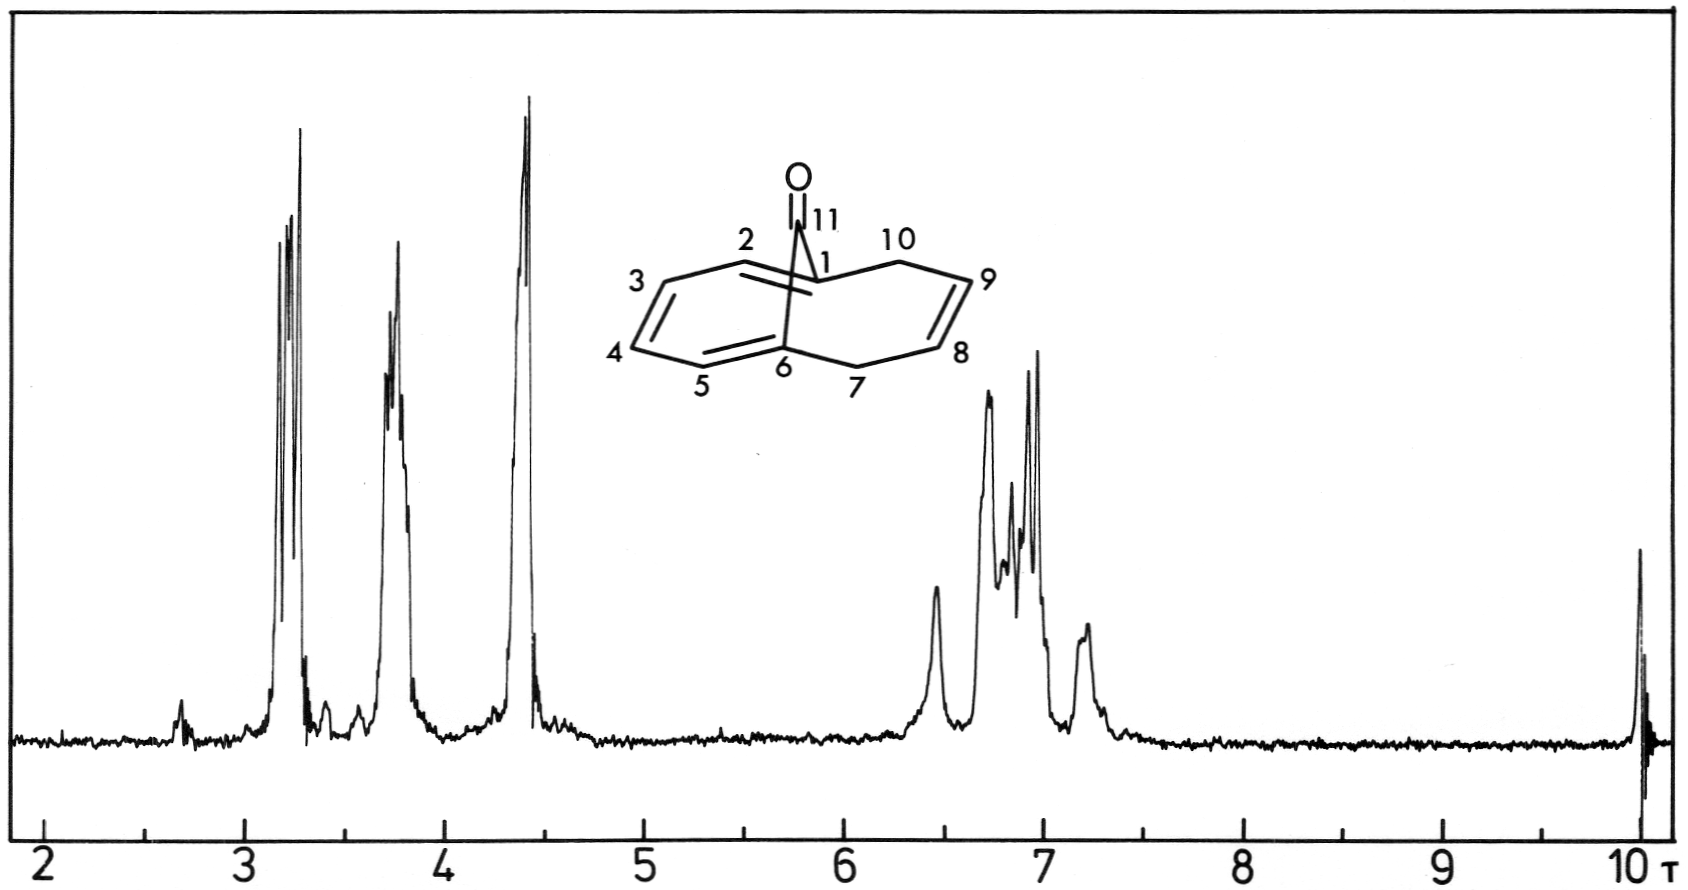
\includegraphics[width=14.29cm]{NMR_021}
\begin{alltt}
Abb. 21: \raise0.5ex\hbox{1}H-NMR-Spektrum des 11-Oxobicyclo[4.4.1]undecatetraens-
(1,3,5‚8) (14) in CDCl\lower0.5ex\hbox{3} (60 MHz; TMS als innerer Standardj


gegenüber dem 11-\underline{endo}-Brombicyclo[4.4.l]undecatetraen-(1‚3,5,8)
(45) fast identische Aufspaltungsmuster und Absorptionslagen zei-
gen. Eine genaue Protonenanalyse des AA'XX'-Systems wurde nach
Vermessen von 100 MHz - Spektren durchgeführt. Dabei stellte sich
heraus, daß die Signale des X-Teils durch Fernkopplung mit der ein-
fach ungesättigten Ringhälfte so stark aufgespalten werden, daß nur
der A-Teil angenähert analysiert werden konnte. Daher sind die er-
haltenen Parameter mit dem relativ großen Fehler von 0.2 Hz behaf-
tet. Die vicinalen Kopplungskonstanten J23 = 5.7 Hz sowie J34 =
11.0 Hz differieren sehr stark, weshalb das Triensystem lokalisier-
te Doppelbindungen und ausgeprägte Bindungsalternanz aufweisen
dürfte. Auch der N-Nert ist mit 5.8 Hz typisch für ein Dyclohepta-
triensystem. Die Verschiebungsdifferenz der Lamorfrequenzen \(\nu\)\lower0.5ex\hbox{A} und
\(\nu\)\lower0.5ex\hbox{B} besitzt mit \(\nu\)\lower0.5ex\hbox{B} \(\delta\) = 0.54 ppm einen wesentlich kleineren Wert als
in den monosubstituierten Verbindungen, in denen sie generell um
0.9 ppm lag. Diese Erscheinung dürfte eine Folge der sp\raise0.5ex\hbox{2}-Hybridi-
sierung des Brückenkohlenstoffatoms in Verbindung mit einem Aniso-
tropieeffekt des Sauerstoffatoms sein. Aus dieser Tatsache analog
zu den Verhältnissen beim 11-Oxo-1,6-methano-[101annulen (15) eine

\newpage
\makebox[0.8\textwidth][c]{- 48 -}


weitgehende Einebnung des Cycloheptatriensegmentes ableiten zu
wollen, bleibt jedoch Spekulation, obwohl auch das UV-Spektrum zu
dieser Hypothese beiträgt. Es weist zwei eng benachbarte Maxima
bei 235 nm und 251 nm mit deutlich höherer Extinktion (\(\epsilon\) = 5600
bzw. 5800) auf.

 

2.3 11-Oxobicyclo[4.4.1lundecatrien-[1‚3,5) (13)

Zur Darstellung der Titelverbindung (13) konnte nicht wie bei der
Synthese des 11-Oxobicyclo[4.4.1]undeoatetraens-(1‚3,5,8) (14) auf
eine Verbindung zurückgegriffen werden, die den Perimeter mit den
erforderlichen Doppelbindungen bereits vorgebildet enthält. Hier
muss ein neues Konzept entwickelt werden, wenn auch die einzelnen
Reaktionsschritte durch frühere Arbeiten des hiesigen Arbeits-
kreises vorgezeichnet sind.

\end{alltt}
%\schemedebug{true}
\schemestart
\hspace{-0.5cm}
% iso-Hexalin (50)
\chemname{
\chemfig{=_[:60]-[:12]-[:-12]
(=_[:-120])% 1 - 6
-[:12]-[:-12]-[:-120]-[:-168]-[:168]-[:-168]-[:168]}
}{\cmpd{isohexalin}}
\arrow(.mid east--.mid west){->[\chemfig{\lewis{4:,C}Br_2}]}[,1.1]
% Hexalindibromcarbenaddukt (51)
\chemname{
\chemfig{=_[:60]-[:12]-[:-12]%
(-[:-120])% Einfachbindung 1 - 6
(-[:-252]?(-[:165]Br)(-[:15]Br))% 1,6 Bruecke
-[:12]-[:-12]-[:-120]-[:-168]-[:168]?-[:-168]-[:168]}%
}{\cmpd{hexalindibromcarbenaddukt}}
\arrow(.mid east--.mid west){->[\textsf{--Br}]}[,1.05]
% Monobromid (52)
\chemname{
\chemfig{=_[:60]-[:12]-[:-12]
(-[:-120])% Einfachbindung 1 - 6
(-[:-252]?(-[:15]Br))% 1,6 Bruecke
-[:12]-[:-12]-[:-120]-[:-168]-[:168]?-[:-168]-[:168]}
}{\cmpd{bromtricyclo11en}}
\schemestop
\\[8pt]
%\schemedebug{true}
\schemestart
\hspace{-0.5cm}
\arrow(.mid east--.mid west){->[\textsf{--2H}]}[,0.7]
% 11-Brom-bicycloundecatrien (53)
\chemname{
\chemfig{=_[:60]-[:12]=_[:-12]
(-[:-252]?(-[:15]Br))% 1,6 Bruecke
-[:12]-[:-12]-[:-120]-[:-168]-[:168]?=_[:-168]-[:168]}
}{\cmpd{bromobicyclo11trien}}
\arrow(.mid east--){->[\parbox[b]{2cm}{\textsf{1.\,AgOAc, 2.\,MeMgJ}}]}[,1.2]
\mbox{~}%
\arrow(--.mid west){->[\hbox{\textsf{3.\,DMSO}}]}[,1.1]
\chemname{
\chemfig{=_[:60]-[:12]=_[:-12]
(-[:-252]?(=[:90,0.6]O))% 1,6 Bruecke
-[:12]-[:-12]-[:-120]-[:-168]-[:168]?=_[:-168]-[:168]}
}{\cmpd{trientroponophan}}
\schemestop
\chemnameinit{}
\begin{alltt}
 
Analog zur Darstellung des aromatischen Ketons (15) beginnt man
mit einem Dibromcarbenaddukt (51), aus dem reduktiv ein Bromatom
entfernt wird. Die anschließende Einführung weiterer Doppelbin-
dungen mit Hilfe dehydrierender Agentien sollte eine Öffnung des
Cyclopropanringes bewirken und zum 11-Brombicyclo[4.4.1]undeca-
trien-(1,3‚5) (53) führen, das in der bekannten Reaktionssequenz
in das Keton (13) überführt wird. Die im Zuge der Synthese auftre-
tende Bildung von Stellungsisomeren, mit der wegen der Nichtäqui-
valenz der beiden Ringhälften gerechnet werden muss, könnte jedoch
Komplikationen durch Trennungsprobleme mit sich bringen.

\newpage
\makebox[0.8\textwidth][c]{- 49 -}


2.3.1 11-Bromtricyclo[4.4.1.0\raise0.5ex\hbox{1,6}]undecaen-3 (52)

Das benötigte Dibromcarbenaddukt an 1,4-Dihydrotetralin (50), das
aus Tetralin durch BIRCH-Reduktion erhalten wird \raise0.5ex\hbox{[103]}, ist in
etwa 12 \%iger Ausbeute zugänglich \raise0.5ex\hbox{[36]}. Nach Erhitzen der reinen
Substanz (51) mit Tri-n-butylzinnhydrid und nachfolgende fraktio-
nierte Destillation im Hochvakuum resultiert ein farbloses Öl, das
laut gaschromatographischer Untersuchung (Säule: Carbowax 20) zwei
neue Verbindungen im Verhältnis 3:2 enthält. Durch verlustreiche
Säulenchromatographie an Aluminiumoxid (Eluens: Pentan) lässt sich
das Gemisch in die Komponenten trennen. Für die weitere Synthese
kann das Isomerengemisch eingesetzt werden, ohne daß Ausbeutever-
luste zu befürchten sind.

\end{alltt}
\schemestart
\hspace{0.25cm}
% Hexalindibromcarbenaddukt (51)
\chemname{
\chemfig{=_[:60]-[:12]-[:-12]%
(-[:-120])% Einfachbindung 1 - 6
(-[:-252]?(-[:165]Br)(-[:15]Br))% 1,6 Bruecke
-[:12]-[:-12]-[:-120]-[:-168]-[:168]?-[:-168]-[:168]}%
}{\cmpd{hexalindibromcarbenaddukt}}
\arrow(.mid east--.mid west){->[\chemfig{n{-}Bu_3SnH}]}[,1.4]
% exo-Monobromid (52a)
\chemname{
\chemfig{=_[:60]-[:12]-[:-12]
(-[:-120]) % Einfachbindung 1 - 6
(-[:-252]?(-[:15]Br))% 1,6 Bruecke
-[:12]-[:-12]-[:-120]-[:-168]-[:168]?-[:-168]-[:168]}
}{\cmpd{bromtricyclo11en.a}}
% invisible shortened arrow to separate compounds and align them
\arrow(.mid east--.mid west){0}[,.2]
% endo-Monobromid (52b)
\chemname{
\chemfig{=_[:60]-[:12]-[:-12]
(-[:-120]) % Einfachbindung 1 - 6
(-[:-252]?(-[:165]Br))% 1,6 Bruecke
-[:12]-[:-12]-[:-120]-[:-168]-[:168]?-[:-168]-[:168]}
}{\cmpd{bromtricyclo11en.b}}
\schemestop
\chemnameinit{}
\begin{alltt}

Beide Verbindungen geben identische Elementaranalysen und besitzen
fast deckungsgleiche IR-Spektren, wie es im Sinne der obigen Reak-
tionsgleichung für die erwarteten Isomere (52) zu fordern ist. An-
hand der \raise0.5ex\hbox{1}H-NMR-Spektren (s. Abb. 22 auF S. 50) ist eine eindeutige
Zuordnung der Isomeren möglich, auch wenn sich nur die Absorptionen
für das Brückenproton und die allylischen Protonen an C-2 und C-5
signifikant unterscheiden. Zieht man nämlich noch das \raise0.5ex\hbox{1}H-NMR-
Spektrum des 11,11-Dibromtricyclo[4.4.1.0\raise0.5ex\hbox{1,6}]undecaens-3 (51) zu-
rate, so ist augenscheinlich das Bromatom über der ungesättigten
Ringhälfte für das Singulett der allylischen Protonen verantwort-
lich. Somit dürfte aber auch in Verbindung (52b) das Bromatom die
\underline{exo}-Konfiguration einnehmen, da dieselbe Erscheinung beobachtet
wird. Für das Isomere (52a) steht damit gleichzeitig die \underline{endo}-
Stellung außer Frage, zumal auch das Brückenproton H-11 bei
\(\tau\) = 6.72 um 0.3 ppm tiefer in Resonanz tritt als im \underline{exo}-Isomeren
(52b), da es zusätzlich durch den Anisotropiekegel der Doppelbin-
dung in geringem Maße entschirmt wird.


\newpage
\makebox[0.8\textwidth][c]{- 50 -}


\end{alltt}
\hspace*{-0.25cm}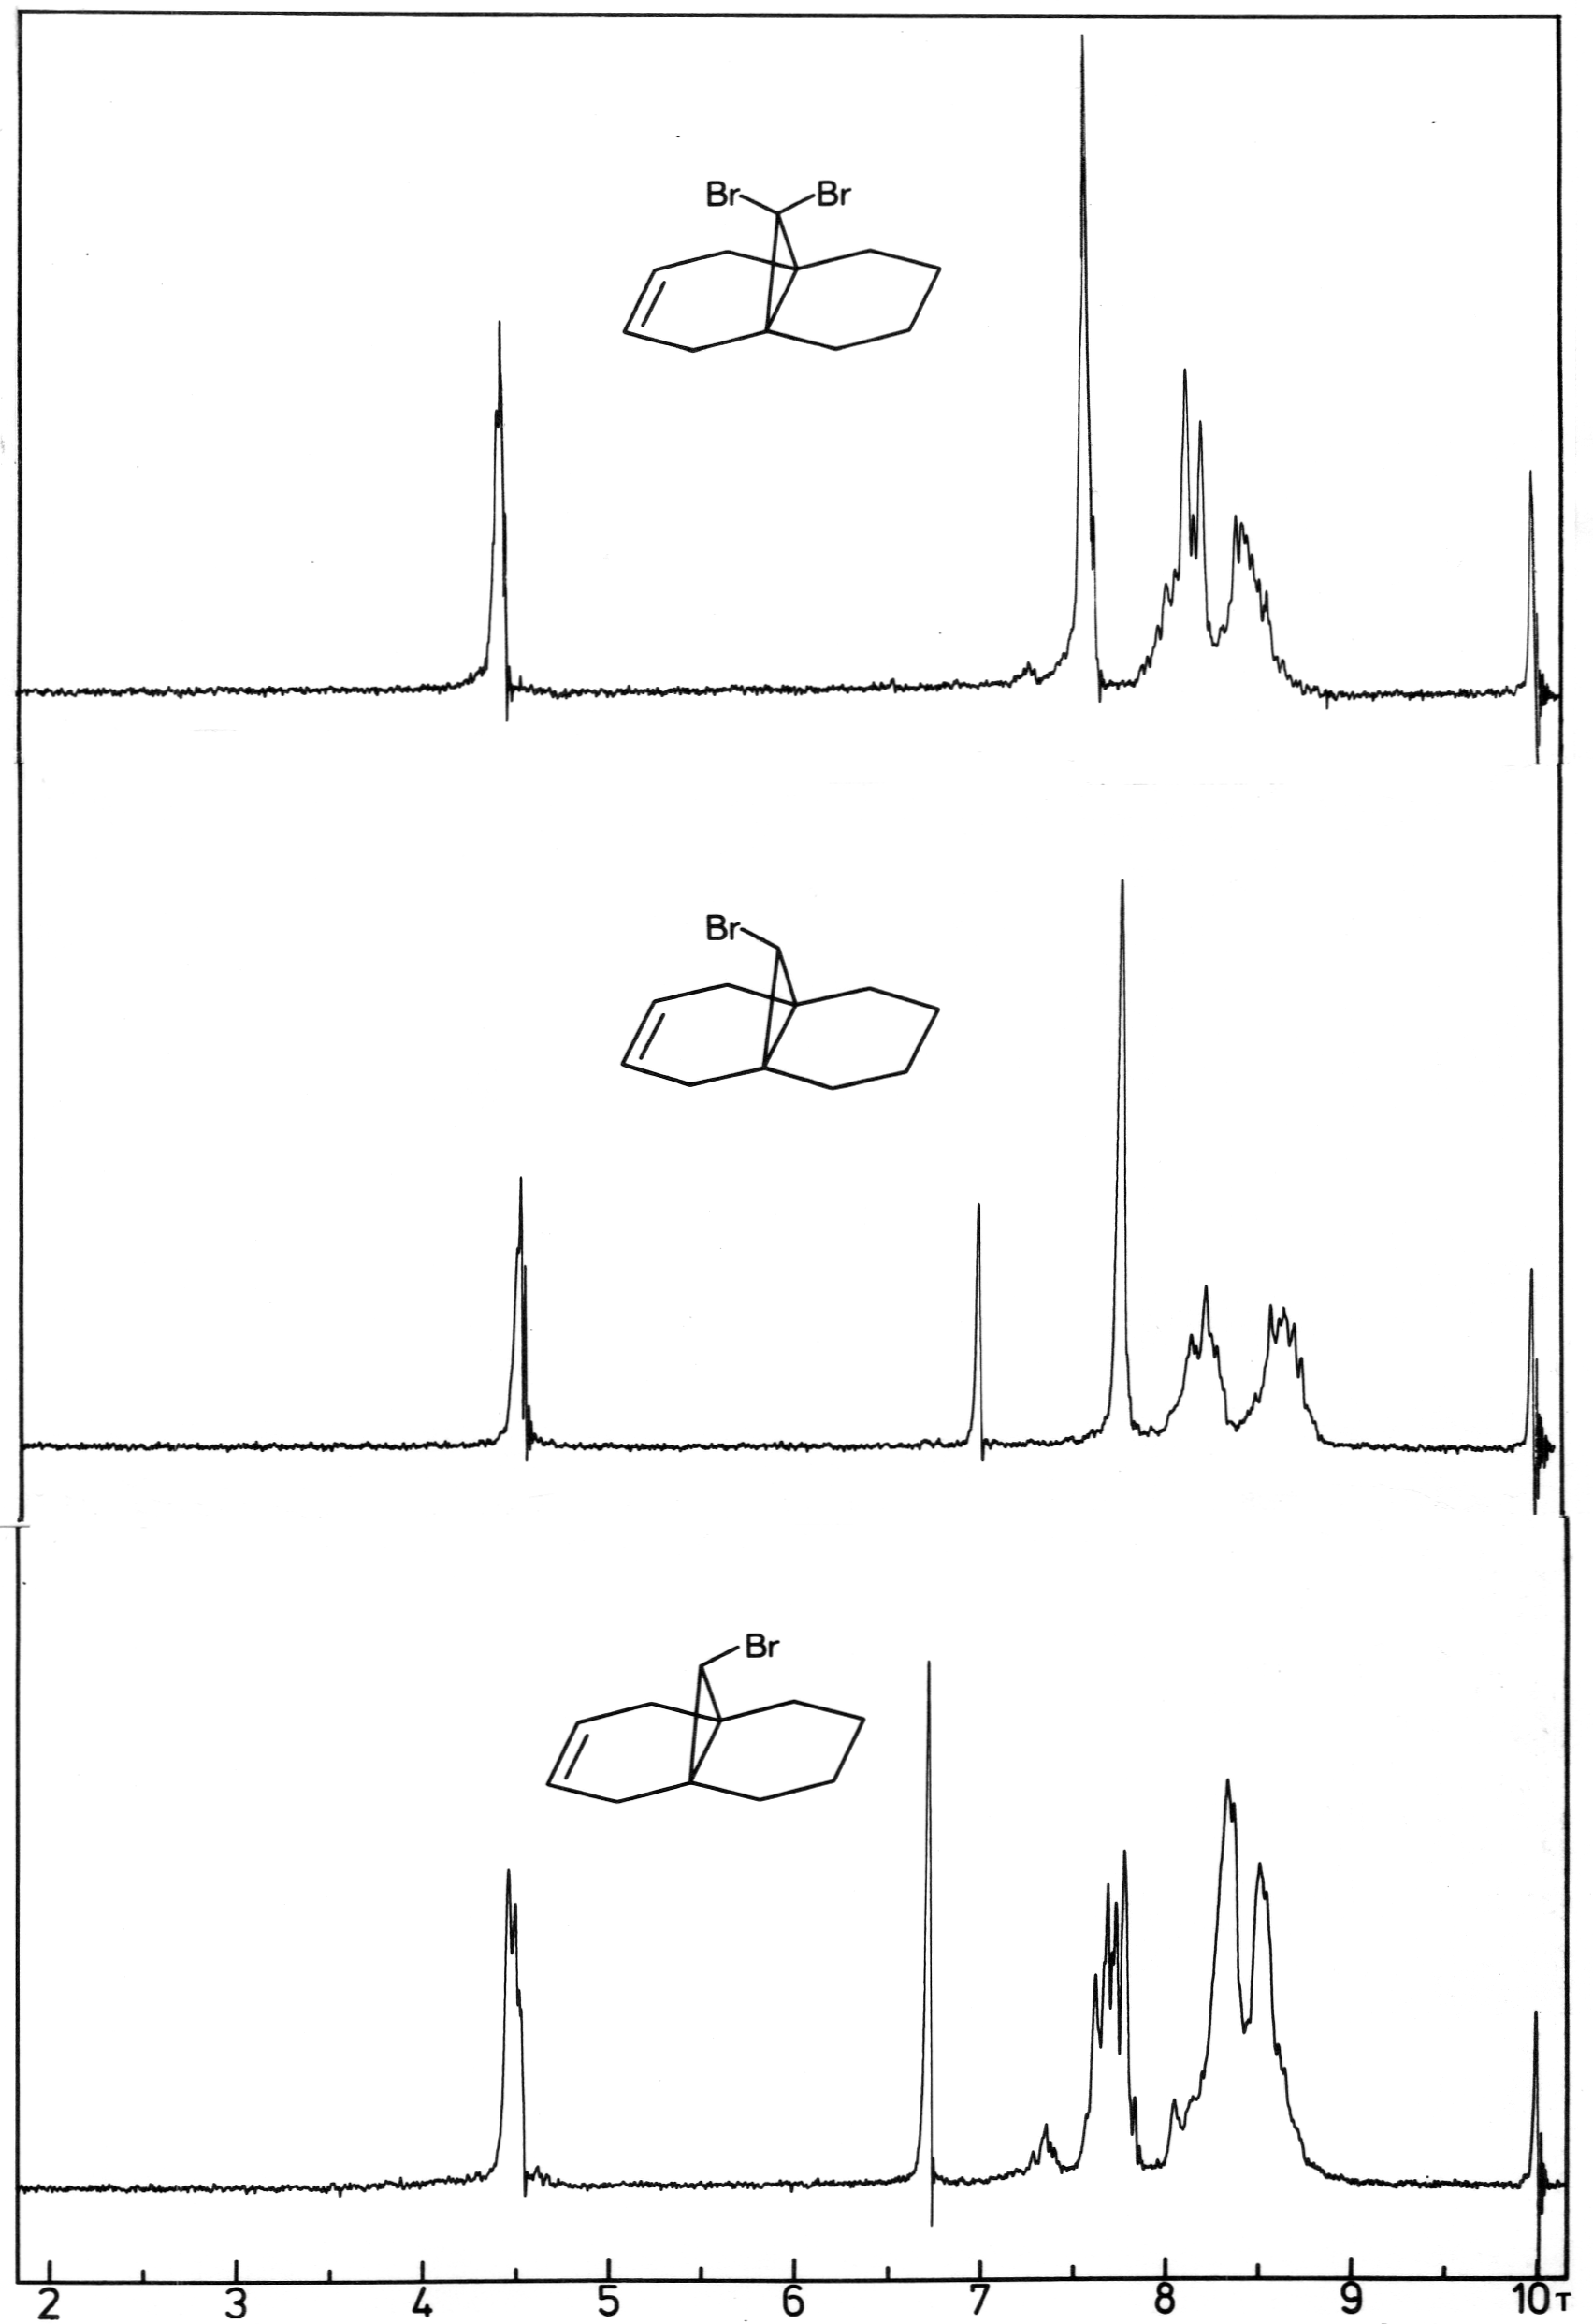
\includegraphics[width=14.42cm]{NMR_022}
\begin{alltt}
Abb. 22: \raise0.5ex\hbox{1}H-NMR-Spektren des 11‚11-Dibromtricyclo[4.4.1.0\raise0.5ex\hbox{1,6}]unde-
caens-3 (51), des 11-\underline{exo}-Bromtricyclo[4.4.1.0\raise0.5ex\hbox{1,6}]undeca-
ans-3 (52b) und des \underline{endo}-Bromids (52a) in CCl\lower0.5ex\hbox{4} (60 MHz;
TMS als innerer Standard)
\newpage
\makebox[0.8\textwidth][c]{- 51 -}


Der Strukturbeweis wurde unabhängig auch auf chemischem Wege ge-
führt, indem man beide Isomere (52) getrennt zum 11-Brombicyclo-
[4.4.1]undecatrien-(1‚3,5) (53) dehydrierte, wobei jeweils ein
Stellungsisomeres entstand, dessen Molekülaufbau sehr einfach
aufgrund der \raise0.5ex\hbox{1}H-NMR-Spektren festzustellen war (vgl. S. 53).

 

2.3.2 11-Brombicyclo[4.4.1]undecatrien-(1‚3,5) (53)

Die zur Dehydrierung ansonsten generell angewandte Methode -
Bromierung und nachfolgende Dehydrobromierung - erscheint aufgrund
früherer Erfahrungen \raise0.5ex\hbox{[42,104]} bei dieser Verbindungsklasse nicht
zweckmäßig. Da jedoch ein 1,4-hydriertes Molekülsegment vorliegt,
empfiehlt sich der Einsatz von DDCh. Die Umsetzung des Bromidge-
misches (52) mit diesem Reagens in siedendem Dioxan führt erwar-
tungsgemäß in 70 \%iger Ausbeute zu den beiden isomeren 11-Brom-
bicyclo[4.4.1]undecatrienen-(l‚3,5) (53), die laut Gaschromatogramm
(Säule: Carbowax 20) jetzt im Verhältnis 3:1 vorliegen. Dies lässt
den Schluss zu, daß sich das \underline{endo}-Isomere (53a) infolge einer höhe-
ren thermodynamischen Stabilität unter den Reaktionsbedingungen
weniger zersetzt.

\end{alltt}
\schemestart
\hspace{0.5cm}
% Monobromid (52)
\chemname{
\chemfig{=_[:60]-[:12]-[:-12]
(-[:-120]) % Einfachbindung 1 - 6
(-[:-252]?(-[:15]Br))% 1,6 Bruecke
-[:12]-[:-12]-[:-120]-[:-168]-[:168]?-[:-168]-[:168]}
}{\cmpd{bromtricyclo11en}}
\arrow(.mid east--.mid west){->[\chemfig{{-2}H}]}
% exo-11-Brom-bicycloundecatrien (53a)
\chemname{
\chemfig{=_[:60]-[:12]=_[:-12]
(-[:-252]?(-[:15]Br))% 1,6 Bruecke
-[:12]-[:-12]-[:-120]-[:-168]-[:168]?=_[:-168]-[:168]}
}{\cmpd{bromobicyclo11trien.a}}
% invisible shortened arrow to separate compounds and align them
\arrow(.mid east--.mid west){0}[,.2]
% endo-11-Brom-bicycloundecatrien (53b)
\chemname{
\chemfig{=_[:60]-[:12]=_[:-12]
(-[:-252]?(-[:165]Br))% 1,6 Bruecke
-[:12]-[:-12]-[:-120]-[:-168]-[:168]?=_[:-168]-[:168]}
}{\cmpd{bromobicyclo11trien.b}}
\schemestop
\chemnameinit{}
\begin{alltt}

Völlig identische Resultate erzielt man überraschenderweise durch
die Verwendung von Selendioxid in wässriger, gepufferter Dioxan-
lösung. Dieses Reagens ist nämlich ebenfalls in der Lage, bei Ver-
bindungen, die das Bicyclo[4.1.0]hepten-3-Fragment enthalten, eine
Dehydrierung herbeizuführen \raise0.5ex\hbox{[105]}. Erstaunlich ist immerhin, daß
keinerlei Ketonbildung zu beobachten ist, obwohl Selendioxid unter
denselben Reaktionsbedingungen z.B. Cycloheptatrien zu Tropon oxi-
diert \raise0.5ex\hbox{[106]}.

\newpage
\makebox[0.8\textwidth][c]{- 52 -}


Für die Synthese erweist es sich als praktisch, eine Isomerentren-
nung auf dieser Stufe durchzuführen. Dazu wird das nach der Umset-
zung anfallende ölige Rohgemisch einer Säulenchrcmatographie an
Aluminiumoxid (Eluens: Pentan) unterworfen. Das als erste Fraktion
isolierte farblose Öl vom Kp = 75 - 77\degree{}C bei 0.45 mm Hg erweist
sich als 11-\underline{endo}-Brombicyclo[4.4.1]undecatrien-(1‚3,5) (53a), wäh-
rend die Substanz mit dem geringeren Rf-Wert kristallines \underline{exo}-
Isomeres (53b) vom Fp = 33 - 34\degree{}C darstellt.

Die Elementaranalysen sprechen für die gleiche Zusammensetzung der


\end{alltt}
\hspace*{-0.25cm}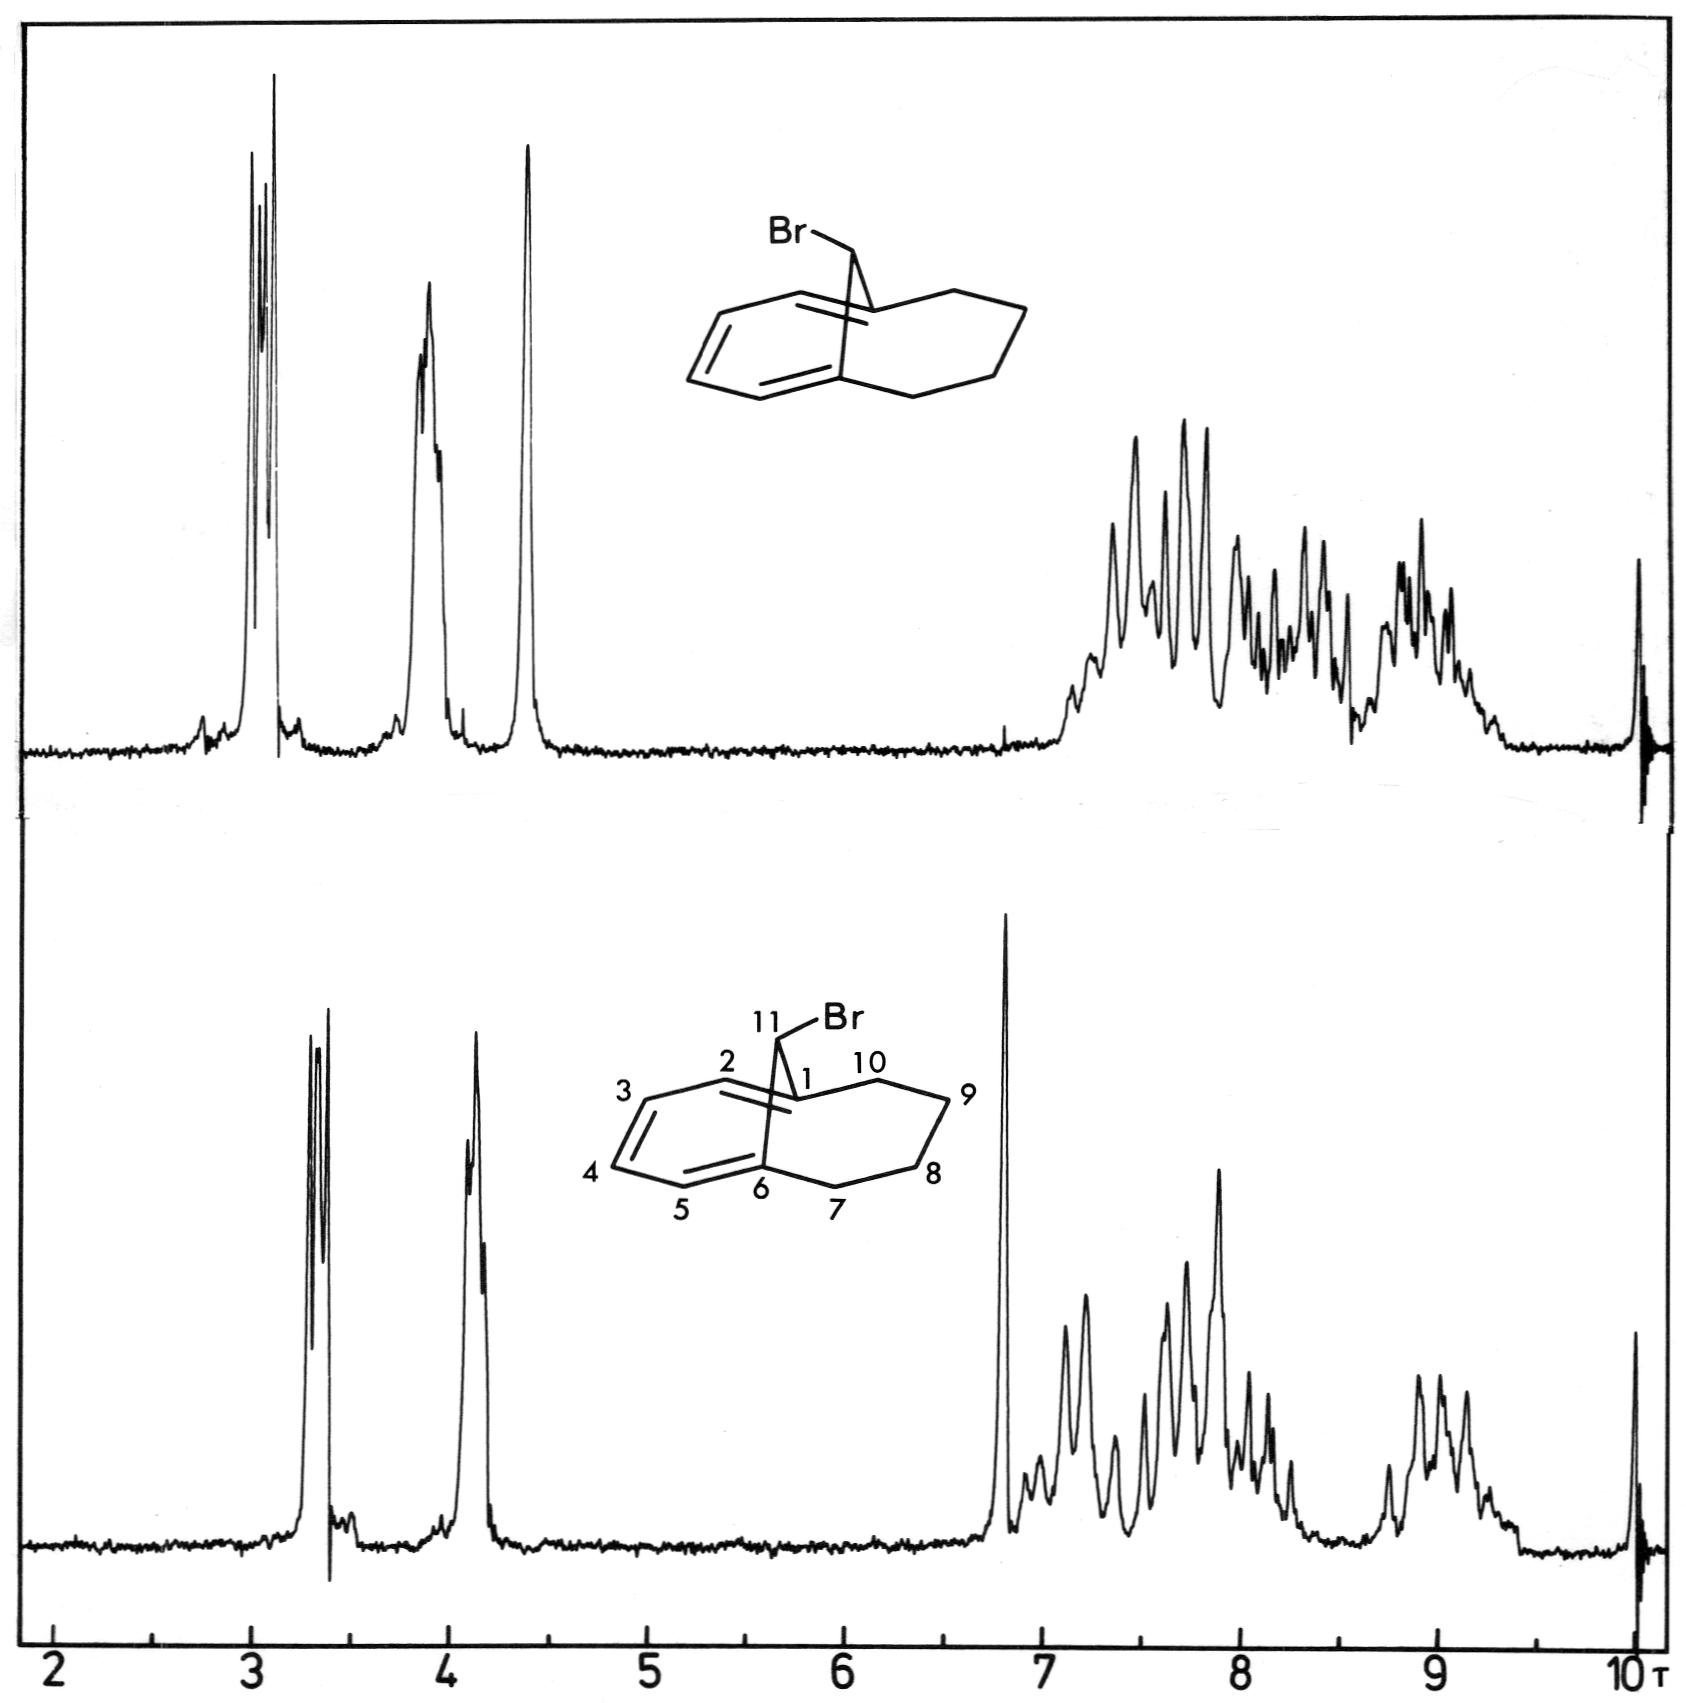
\includegraphics[width=14.275cm]{NMR_023}
\begin{alltt}
Abb. 23: \raise0.5ex\hbox{1}H-NMR-Spektren des 11-\underline{exo}-Brombicyclo[4.4.1]undeca-
triens-(1,3,5) (53b) in CDCl\lower0.5ex\hbox{3} und des \underline{endo}-Bromids (53a)
in CCl\lower0.5ex\hbox{4} (60 MHz; TMS als innerer Standardi
\newpage
\makebox[0.8\textwidth][c]{- 53 -}


beiden Isomeren (53); die IR-Spektren sind wegen ihrer Ähnlichkeit
für die Strukturzuordnung nur von geringem diagnostischen Wert.

In den \raise0.5ex\hbox{1}H-NMR-Soektren (e. Abb. 23 auf s. 52) geben die olefini-
schen Protonen H-2 - H-5 jeweils Anlass zu einem AA'XX'-System
zentriert bei \(\tau\) = 3.6, während die Protonen des gesättigten Ring-
teils bei \(\tau\) = 6.7 - 9.4 als komplexes Multiplett erscheinen. Trotz
der weitgehenden Übereinstimmung unterscheiden sich die Spektren
in einem wichtigen Detail, der Absorptionslage des Brückenprotons
H-11‚ die in einem Bereich von 2.4 ppm variiert. Infolge der ste-
rischen und elektronischen Besonderheiten der Moleküle lässt sich
aus dieser Shiftdifferenz die exakte Struktur der Isomeren (53)
ableiten. Das Brückenproton liegt nämlich im 11-\underline{endo}-Brombicyclo-
[4.4.1]undecatrien-(1‚3,5) (53a) über der \(\pi\)-Elektronenwolke des
Trienteils in Richtung der pz-Drbitale und wird infolgedessen
stark abgeschirmt (\(\tau\) = 6.78), während im \underline{exo}-Isomeren (53b) der
entschirmende Effekt des Bromatoms ungehindert einwirken kann,
so daß die Absorption bei tiefem Feld (\(\tau\) = 4.40) eintritt. Bei
bekannter Molekülgeometrie lassen sich die Isomeren (53) auch an-
hand des N-Wertes charakterisieren, der im \underline{endo}-Isomeren (53a) wie
im ll-\underline{endo}-Brombicyclo[4.4.ljundecatetraen-(l‚3,5,8) [45) bei 5.5
Hz liegt, wohingegen er im \underline{exo}-Isomeren (53b) mit 6.5 Hz deutlich
größer ist.

Signifikante Unterschiede lassen sich auch in den Elektronenspek-
tren feststellen: Wie beim analogen Tetraen (45] weist das \underline{endo}-
Isomere (53a) nur eine Schulter bei 253 nm (\(\epsilon\) = 5500) auf. Das
11-\underline{exo}-Brombicyclo[4.4.1]undeoatrien-(1‚3,5) (53b) zeigt dagegen
ein Maximum bei 234 nm mit der hohen Extinktion von 13300 sowie
zwei Schultern bei 262 nm (\(\epsilon\) = 5800) und 305 nm (\(\epsilon\) = soo).


2.3.3 11-\underline{endo}-Aoetoxybicyclo[4.d.1]undecatrien-(1‚3,5) (54)

Zur Präparierung des 11-\underline{endo}-Acetoxybicyclo[4.4.1]undecatriens-
(1,3‚5) (54) geht man von reinem \underline{endo}-Bromid (53a) aus, das durch
Säulenchromatographie durchaus im 20 g - Maßstab zu erhalten ist.

\newpage
\makebox[0.8\textwidth][c]{- 54 -}


Ein Einsatz des rohen Isomerengemisches (53) erweist sich als wenig
zweckmäßig, da wegen des zusätzlichen Auftretens von Zersetzungs-
produkten der labileren \underline{exo}-lsomeren die Ausbeute an Acetat (54)
unnötig erniedrigt wird. Außerdem erfolgt der Brom-Acetat-Austausch
mit Silber(I)acetat in siedendem Eisessig aus denselben Gründen wie
beim Tetraen (46) mit 100 \%iger Retention (vgl. S. 40 f.), so daß
bei Verwendung von isomerenreinem Edukt (53a) komplizierte Reini-
gungsmethoden entfallen. Das Reaktionsgemisch wird nach Filtration
mit Wasser/Pentan aufgearbeitet, wobei nach Umkristallisieren aus
Petroläther das 11-\underline{endo}-Acetoxybicyclo[4.4.1]undecatrien-(1‚3,5)
(54) in Form weißer Nadeln vom Fp = 55 - 56\degree{}C anfällt.

\end{alltt}
\schemestart
\hspace{1.5cm}
% exo-11-Brom-bicycloundecatrien (53a)
\chemname{
\chemfig{=_[:60]-[:12]=_[:-12]
(-[:-252]?(-[:15]Br))% 1,6 Bruecke
-[:12]-[:-12]-[:-120]-[:-168]-[:168]?=_[:-168]-[:168]}
}{\cmpd{bromobicyclo11trien.a}}
\arrow(.mid east--.mid west){->[\textsf{AgOAc}]}[,1.2]
% exo-11-Acetoxy-bicycloundecatrien (54)
\chemname{
\chemfig{=_[:60]-[:12]=_[:-12]
(-[:-252]?(-[:15]OCOCH_3))% 1,6 Bruecke
-[:12]-[:-12]-[:-120]-[:-168]-[:168]?=_[:-168]-[:168]}
}{\cmpd{acetoxybicyclo11trien}}
\schemestop
\chemnameinit{}
\begin{alltt}

Elementaranalyse und IR-Spektrum entsprechen den Erwartungen. Die
Präsenz der Acetatgruppe lässt sich anhand der intensiven Banden
für die Carbonylvalenz bei 1752 cm\raise0.5ex\hbox{-1} und der Schwingung bei \(\tilde{\nu}\)\lower0.5ex\hbox{C-O} =
1236 cm\raise0.5ex\hbox{-1} nachweisen.


\end{alltt}
\hspace*{-0.25cm}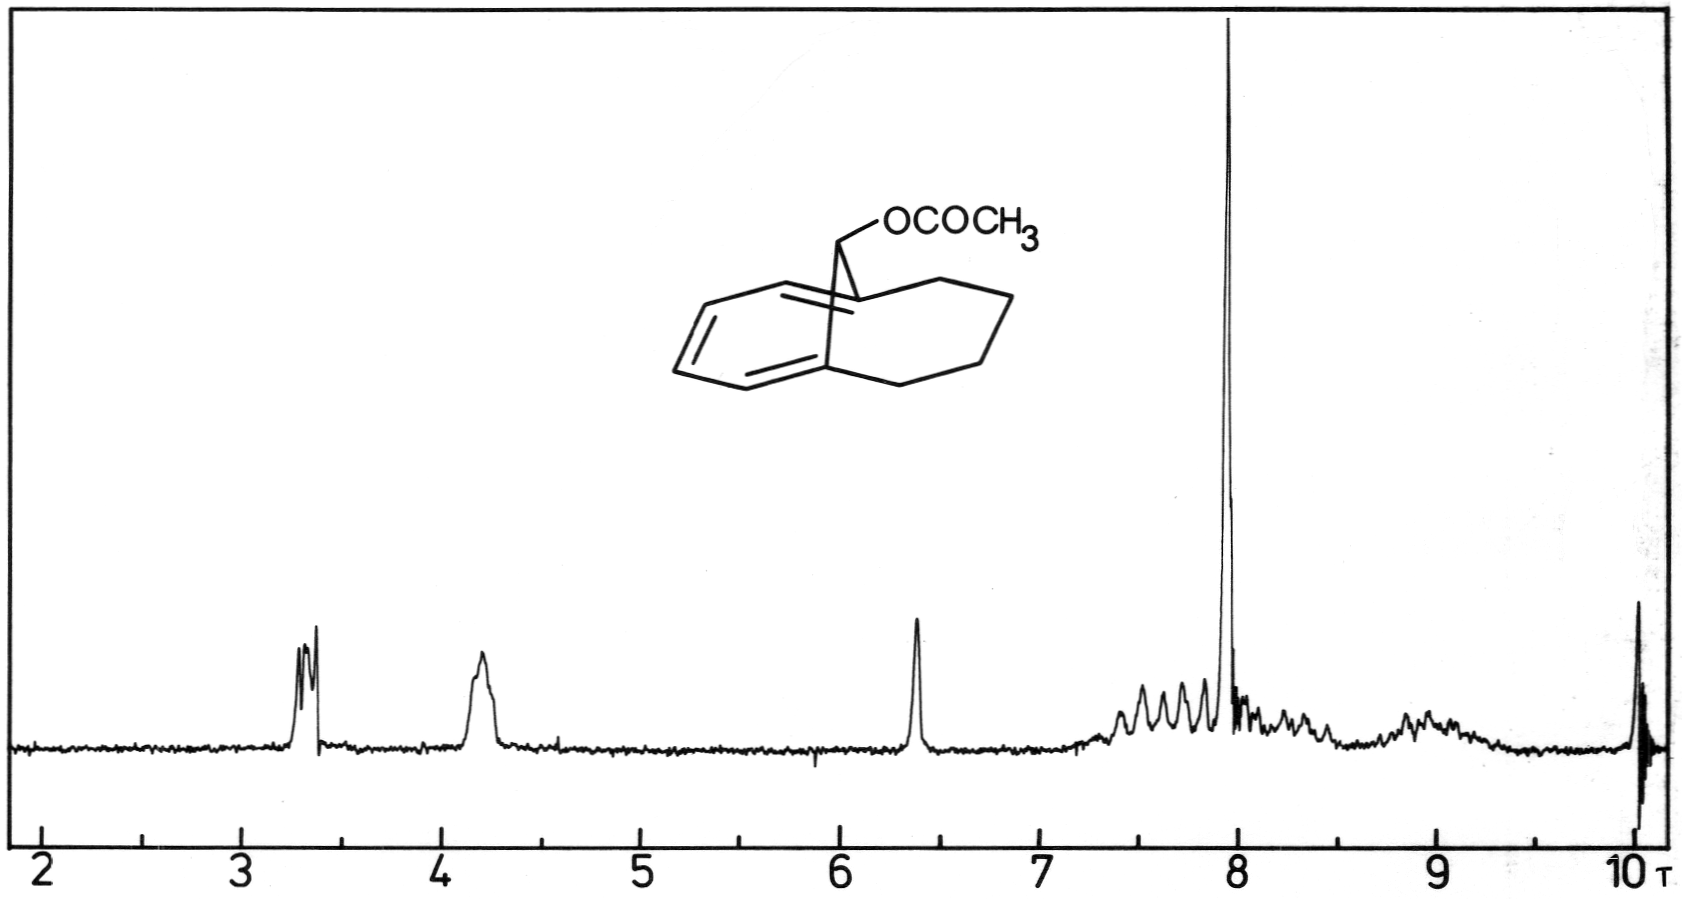
\includegraphics[width=14.24cm]{NMR_024}
\begin{alltt}
Abb. 24: \raise0.5ex\hbox{1}H-NMR-Spektrum des 11-\underline{endo}-Acetoxybioyclo[4.4.1]undeca-
triens-(1,3‚5) (54) in (CCl\lower0.5ex\hbox{4} (60 MHz; TMS als innerer
Standard)
\newpage
\makebox[0.8\textwidth][c]{- 55 -}


Der Erhalt der \underline{endo}-Konfiguration folgt aus der hohen Absorptions-
lage des Brückenprotons bei \(\tau\) = 6.38 und dem niedrigen N-Wert von
5.5 Hz. Weitere Signalgruppen im \raise0.5ex\hbox{1}H-NMR-Spektrum (s. Abb. 24 auF
S. 54) sind das AA'XX'-System für die Trienprotonen H-2 - H-5 bei
\(\nu\)\lower0.5ex\hbox{A} = 3.32\(\tau\) bzw. \(\nu\)\lower0.5ex\hbox{X} = 4.20\(\tau\) und das komplexe Multiplett der ali-
cyclischen Protonen an C-7 - C-10 im Bereich von \(\tau\) = 7.1 - 9.4.
Die Methylgruppe des Substituenten tritt als scharfes Singulett
bei \(\tau\) = 7.93 in Resonanz.

Auch das UV-Spektrum gibt die endo-Struktur mit einem Maximum bei
252 nm (\(\epsilon\) = 5500) befriedigend wieder.

 

2.3.4 11-\underline{endo}-Hydroxybicyclo[4.4.1]undecetrien-(i‚3,5) (55)

Die Umsetzung des 11-\underline{endo}-Acetoxybicyclo[4.4.1]undecatriens-(1‚3,5)
(54) mit Methylmagnesiumjodid in Äther ergibt erwartungsgemäß das
11-\underline{endo}-Hydroxybicyclo[4.4.1]undecatrien-(1‚3,5) (55) in 46 \%iger
Ausbeute. Verlustreiches Umkristallisieren aus Äther/Hexan führt
zu rhombischen, temperaturlabilen Kristallen mit dem Schmelzpunkt
72 - 73\degree{}C.

\end{alltt}
\schemestart
\hspace{1.5cm}
% exo-11-Acetoxy-bicycloundecatrien (54)
\chemname{
\chemfig{=_[:60]-[:12]=_[:-12]
(-[:-252]?(-[:15]OCOCH_3))% 1,6 Bruecke
-[:12]-[:-12]-[:-120]-[:-168]-[:168]?=_[:-168]-[:168]}
}{\cmpd{acetoxybicyclo11trien}}
\arrow(.mid east--.mid west[xshift=5mm]){->[\textsf{MeMgJ}]}[,1.2]
% exo-11-Hydroxy-bicycloundecatrien (55)
\chemname{
\chemfig{=_[:60]-[:12]=_[:-12]
(-[:-252]?(-[:15]OH))% 1,6 Bruecke
-[:12]-[:-12]-[:-120]-[:-168]-[:168]?=_[:-168]-[:168]}
}{\cmpd{hydroxybicyclo11trien}}
\schemestop
\chemnameinit{}
\begin{alltt}

Der Austausch der funktionellen Gruppe lässt sich im IR-Spektrum
mit der breiten Bande bei \(\tilde{\nu}\)\lower0.5ex\hbox{O-H} = 3265 cm\raise0.5ex\hbox{-1} (Valenzschwingung der
Wasserstoffbrücken) und dem Signal bei \(\tilde{\nu}\)\lower0.5ex\hbox{C-O} = 1076 cm\raise0.5ex\hbox{-1} belegen.

Der Habitus des \raise0.5ex\hbox{1}H-NMR-Spektrums (s. Abb. 25 auF S. 56) hat sich
gegenüber dem 11-\underline{endo}-Brombicyclo[4.4.1]undecatrien-(1‚3,5) (53)
nur unwesentlich geändert, zeigt aber weiterhin die Effekte der
\underline{endo}-Substitution sehr deutlich. So tritt das Proton H-11 mit \(\tau\) =
7.25 bei hohem Feld in Resonanz. Das Singulett bei \(\tau\) = 7.35 muss
wegen der charakteristischen Austauschphänomene bei Zusatz von
\newpage
\makebox[0.8\textwidth][c]{- 56 -}


\end{alltt}
\hspace*{-0.25cm}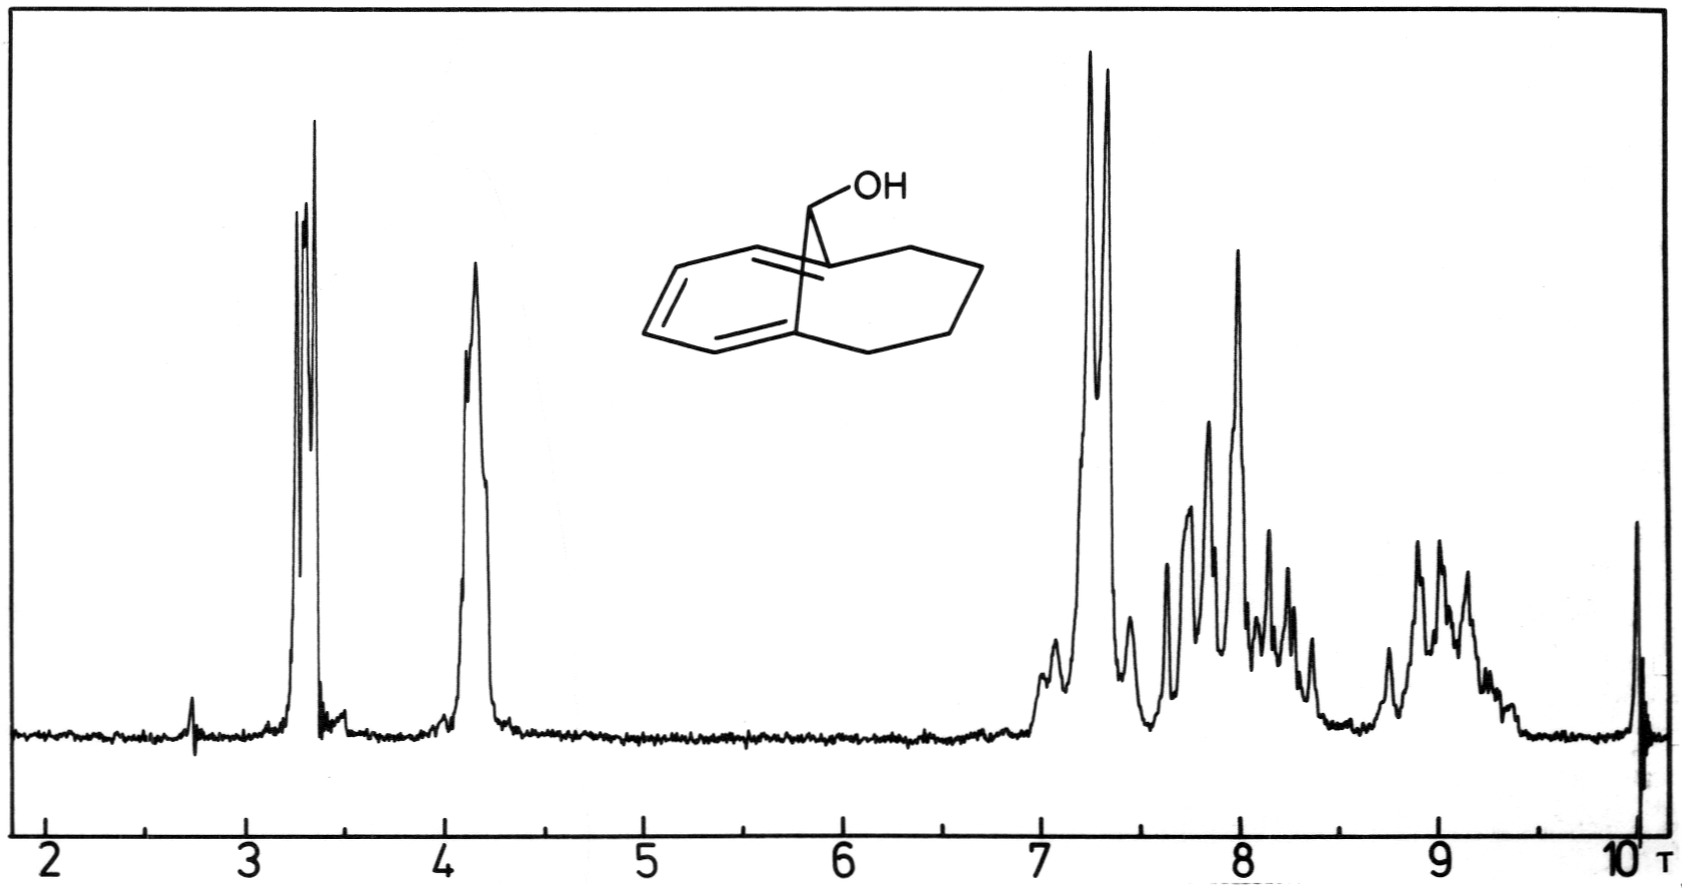
\includegraphics[width=14.24cm]{NMR_025}
\begin{alltt}
Abb. 25: \raise0.5ex\hbox{1}H-NMR-Spektrum des 11-\underline{endo}-Hydroxybicyclo[4.4.1]undeca-
triens-(1,3,5) (55) in CDCl\lower0.5ex\hbox{3} (60 MHz; TMS als innerer
Standard)

 
schwerem Wasser dem Alkoholproton zugeschrieben werden.

Das Maximum im UV-Spektrum bei \(\lambda\)\lower0.5ex\hbox{max} = 255 nm (\(\epsilon\) = 5200) hat sich
im Vergleich zum \underline{endo}-Acetat (54) nur geringfügig bathochrom ver-
schoben. Dies ist ein weiteres Indiz für die Unversehrtheit des
Chromophors.

2.3.5 11-Oxobicyclo[4.4.1]undecatrien-(1‚3,5) (13)

Auch bei diesem etwas labilen Alkohol (55) bewährt sich die Oxi-
dation mit DMSO/Äthyl-[3-(dimethylamino)propyl]carbodiimid-hydro-
chlorid/PTFA vorzüglich. Verfolgt man die Umsetzung dünnschicht-
chromatographisch, so stellt man eine gegenüber dem Tetraen-
Alkohol (47] merklich beschleunigte Reaktionsgeschwindigkeit fest,
da anscheinend die nunmehr völlig gesättigte Ringhälfte die Annähe-
rung des Reaktanden sterisch weniger behindert. Wässrig-ätherische
Aufarbeitung nach 24-stündiger Reaktion liefert das Rohprodukt in
90 - 100 \%iger Ausbeute als weiße Kristalle, die nach dem Umkri-
\newpage
\makebox[0.8\textwidth][c]{- 57 -}


stallisieren als Nadeln mit dem Schmelzpunkt 63 - 65\degree{}C vorliegen.

\end{alltt}
\schemestart
\hspace{1.5cm}
% exo-11-Hydroxy-bicycloundecatrien (55)
\chemname{
\chemfig{=_[:60]-[:12]=_[:-12]
(-[:-252]?(-[:15]OH))% 1,6 Bruecke
-[:12]-[:-12]-[:-120]-[:-168]-[:168]?=_[:-168]-[:168]}
}{\cmpd{hydroxybicyclo11trien}}
\arrow(.mid east--.mid west){->[\raise1.5pt\hbox{\textsf{DMSO}}]}
% 11-Oxo-1,6-methano-undecatrien (13)
\chemname{
\chemfig{=_[:60]-[:12]=_[:-12]
(-[:-252]?(=[:90,0.6]O))% 1,6 Bruecke
-[:12]-[:-12]-[:-120]-[:-168]-[:168]?=_[:-168]-[:168]}
}{\cmpd{trientroponophan}}
\schemestop
\chemnameinit{}
\begin{alltt}

Die Elementaranalyse sichert die Summenformel C11H12O. Mithin muss
ein Keton vorliegen, da im Infrarotspektrum die starke Bande der
Carbonylschwingung bei \(\tilde{\nu}\)\lower0.5ex\hbox{C=O} = 1729 cm\raise0.5ex\hbox{-1} dominiert. Dieser Wert ist
um 11 cm\raise0.5ex\hbox{-1} niedriger als in den beiden anderen Ketonen (14) und
(15), so daß der Winkel C1-C11-C6 aufgeweitet sein muss.


\end{alltt}
\hspace*{-0.25cm}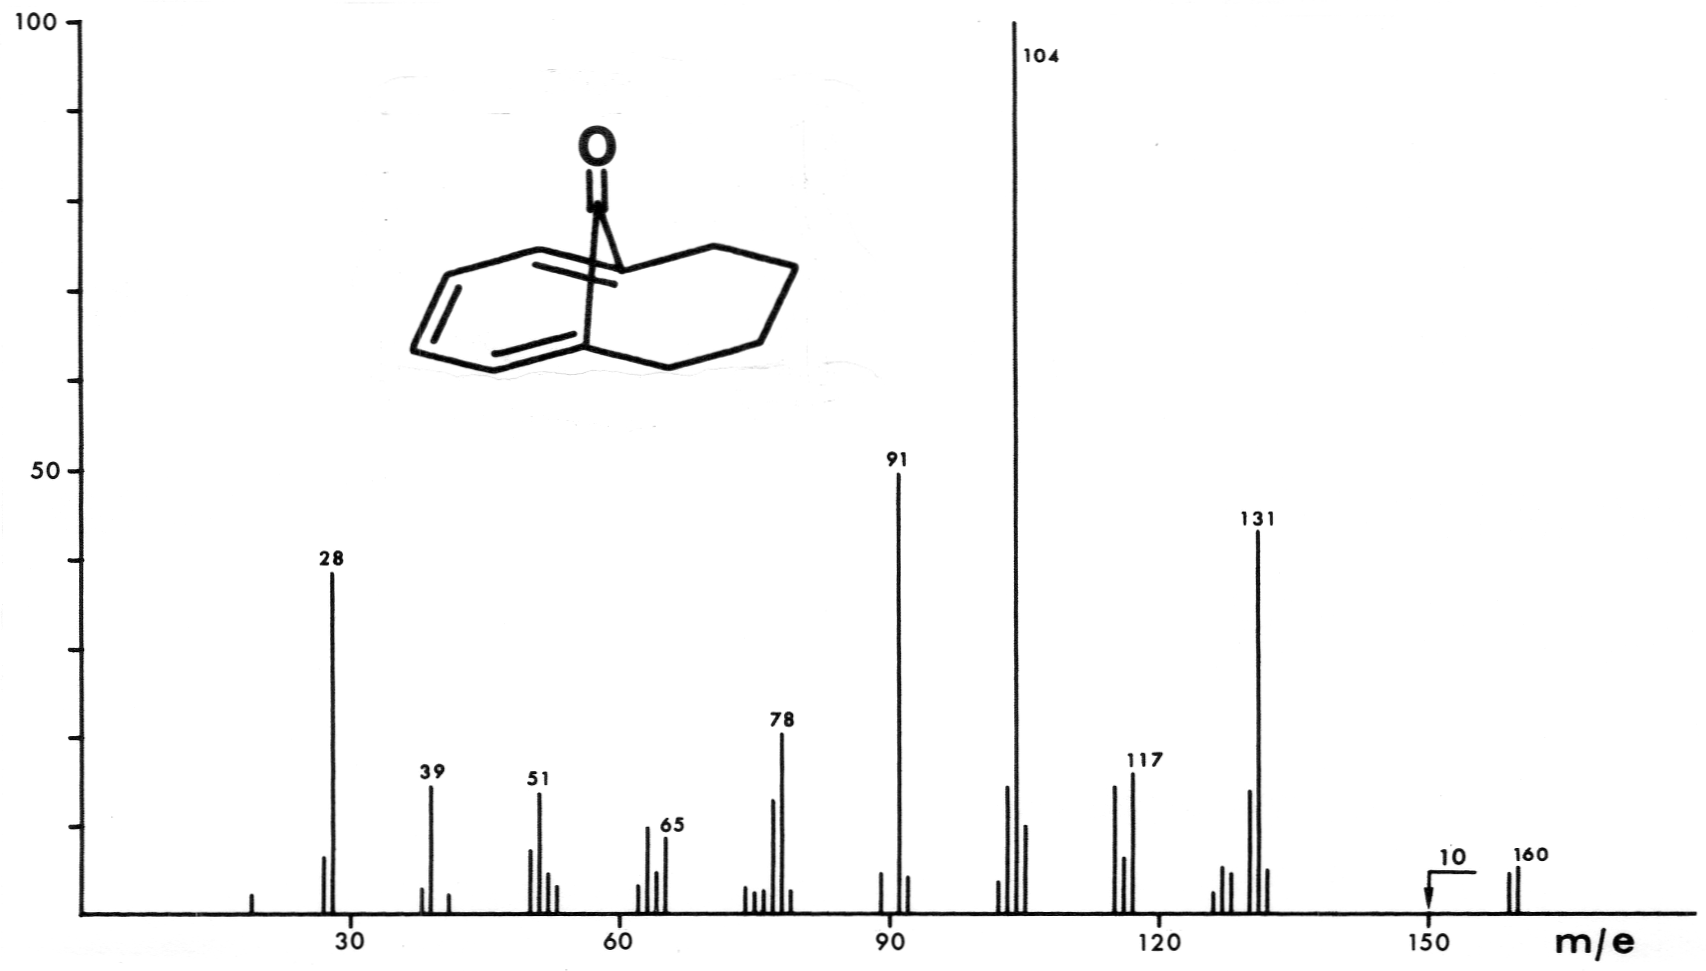
\includegraphics[width=14.444cm]{MASS_026}
\begin{alltt}
Abb. 26: Massenspektrum des 11-Oxobicyclo[4.4.1]undeca-
triens-(1,3,5) (13) (100 eV)

Erwartungsgemäß zeigt das Massenspektrum nur einen unscheinbaren
Molekülpeak bei m/e = 160 (rel. Int. 0.5 \%). In dem komplizierten
Fragmentierungsmuster lassen sich drei Hauptzerfallswege erkennen.

Die Abspaltung von Kohlenmonoxid verläuft erstaunlicherweise nur
in untergeordnetem Maße, erkenntlich an einem Signal mittlerer
Intensität für ein Tetralinkation bei m/e = 131 (43 \%). Auch der
zusätzliche, für das "Tetraen-Keton" (14) diskutierte Fragmentie-
rungsgang, der vom Molekülion durch Ketenabspaltung zum Indenyl-

\newpage
\makebox[0.8\textwidth][c]{- 58 -}


\end{alltt}
\hspace*{0.25cm}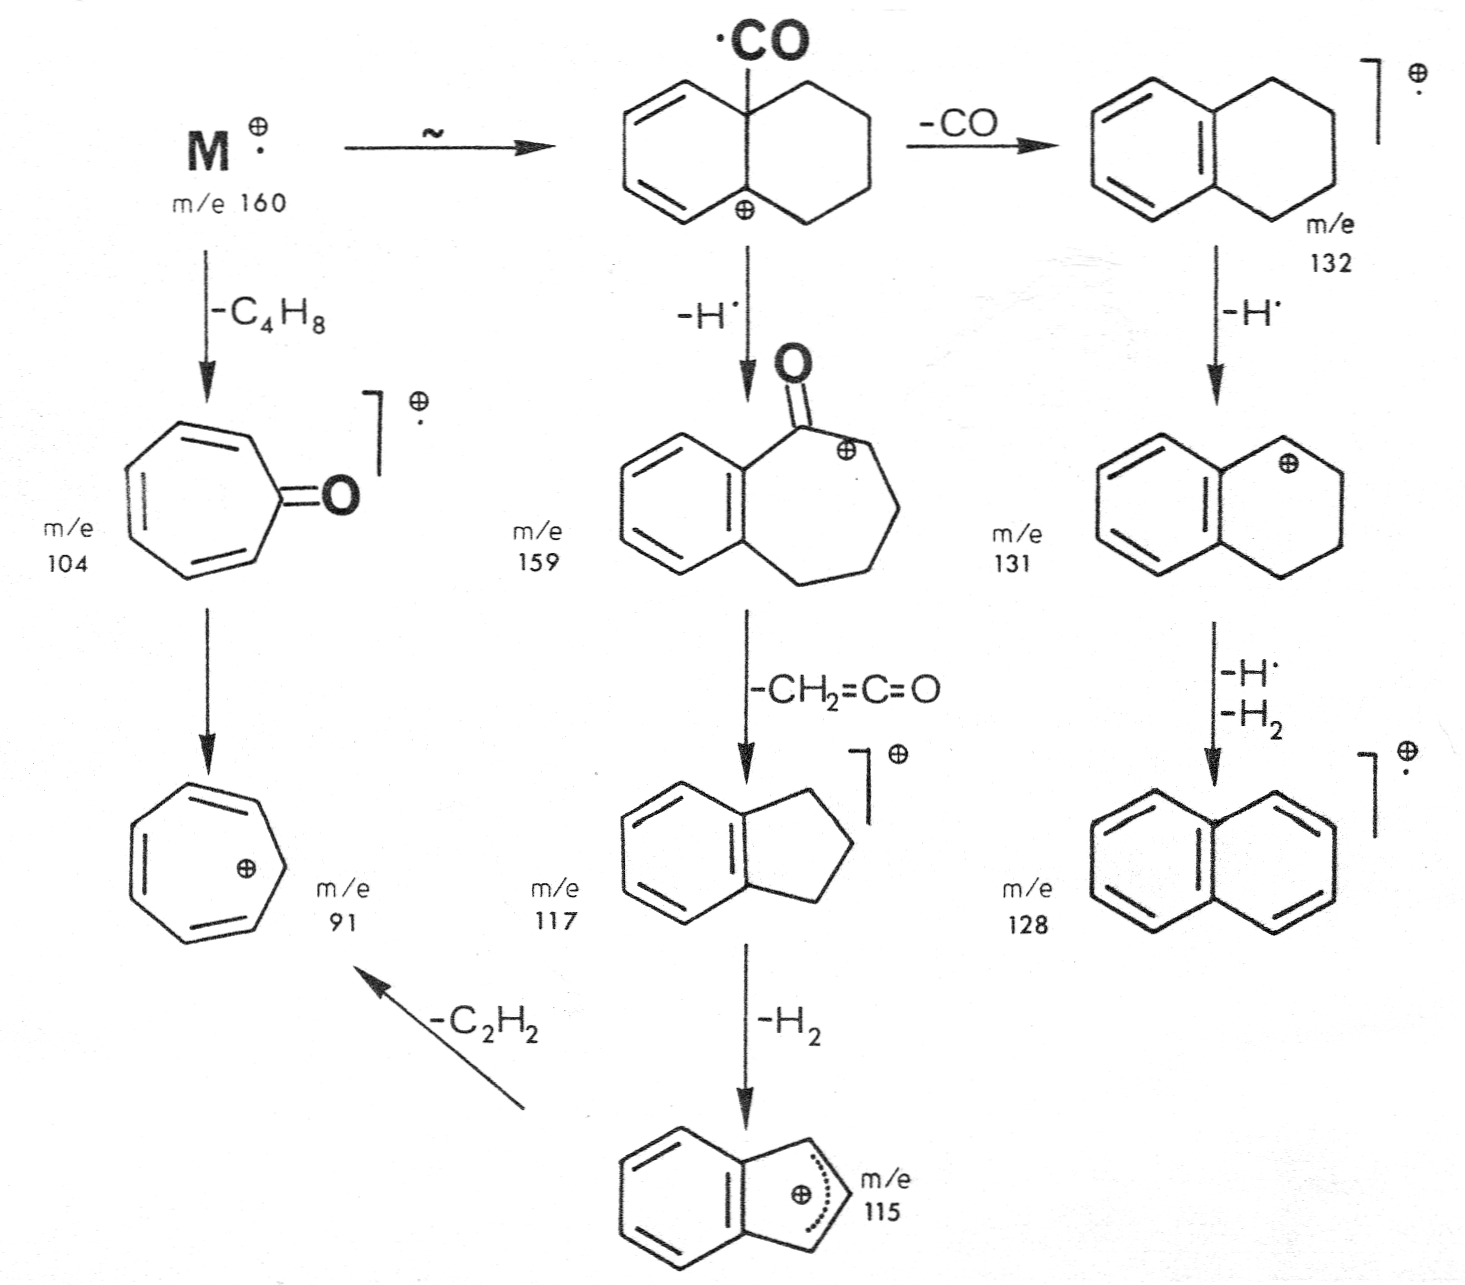
\includegraphics[width=12.4cm]{SCHEMA_004}
\begin{alltt}
Schema 4: Fragmentierungsverlauf des 11-Oxobicyclo[4.4.1]undeca-
triens-(1,3,5) (13) im Massenspektrum

kation bei m/e = 115 (15 \%) führt, ist ohne größere Bedeutung.
Favorisiert ist vielmehr die Bildung von Tropon (Basispeak bei
m/e = 104), das durch die einmalige Abspaltung der gesamten Tetra-
methylenbrüoke entsteht.

Symmetrie- und strukturbedingt zeigt das \raise0.5ex\hbox{1}H-NMR-Spektrum (s. Abb.
27 auf S. 59) nur zwei Signalgruppen für die Perimeterprotonen.
So treten die Wasserstoffatome H-2 - H-5 als AA'XX'-System bei
\(\tau\) = 3.12 - 4.05 in Resonanz. Der A-Teil des Protonensystems absor-
biert dabei mit \(\nu\)\lower0.5ex\hbox{A} = 3.33\(\tau\) an gewohnter Stelle, während die Absorp-
tionslage des X-Teils abhängig von der Brückensubstitution vari-
iert und jetzt bei \(\nu\)\lower0.5ex\hbox{X} = 3.83\(\tau\) liegt. Verglichen mit dem 11-Oxo-
bicyclo[4.4.1]undeoatetraen-(1‚3,5,8] (14) ist die Shiftdifferenz
mit \(\nu\)\lower0.5ex\hbox{o}\(\delta\) = 0.5 ppm weiter gesunken, so daß sich mit der zusätzli-
chen Information aus dem IR-Spektrum über die Aufweitung des Brük-
kendiederwinkels eine höhere Planarität des "Troponsegmentes"
\newpage
\makebox[0.8\textwidth][c]{- 59 -}


\end{alltt}
\hspace*{-0.25cm}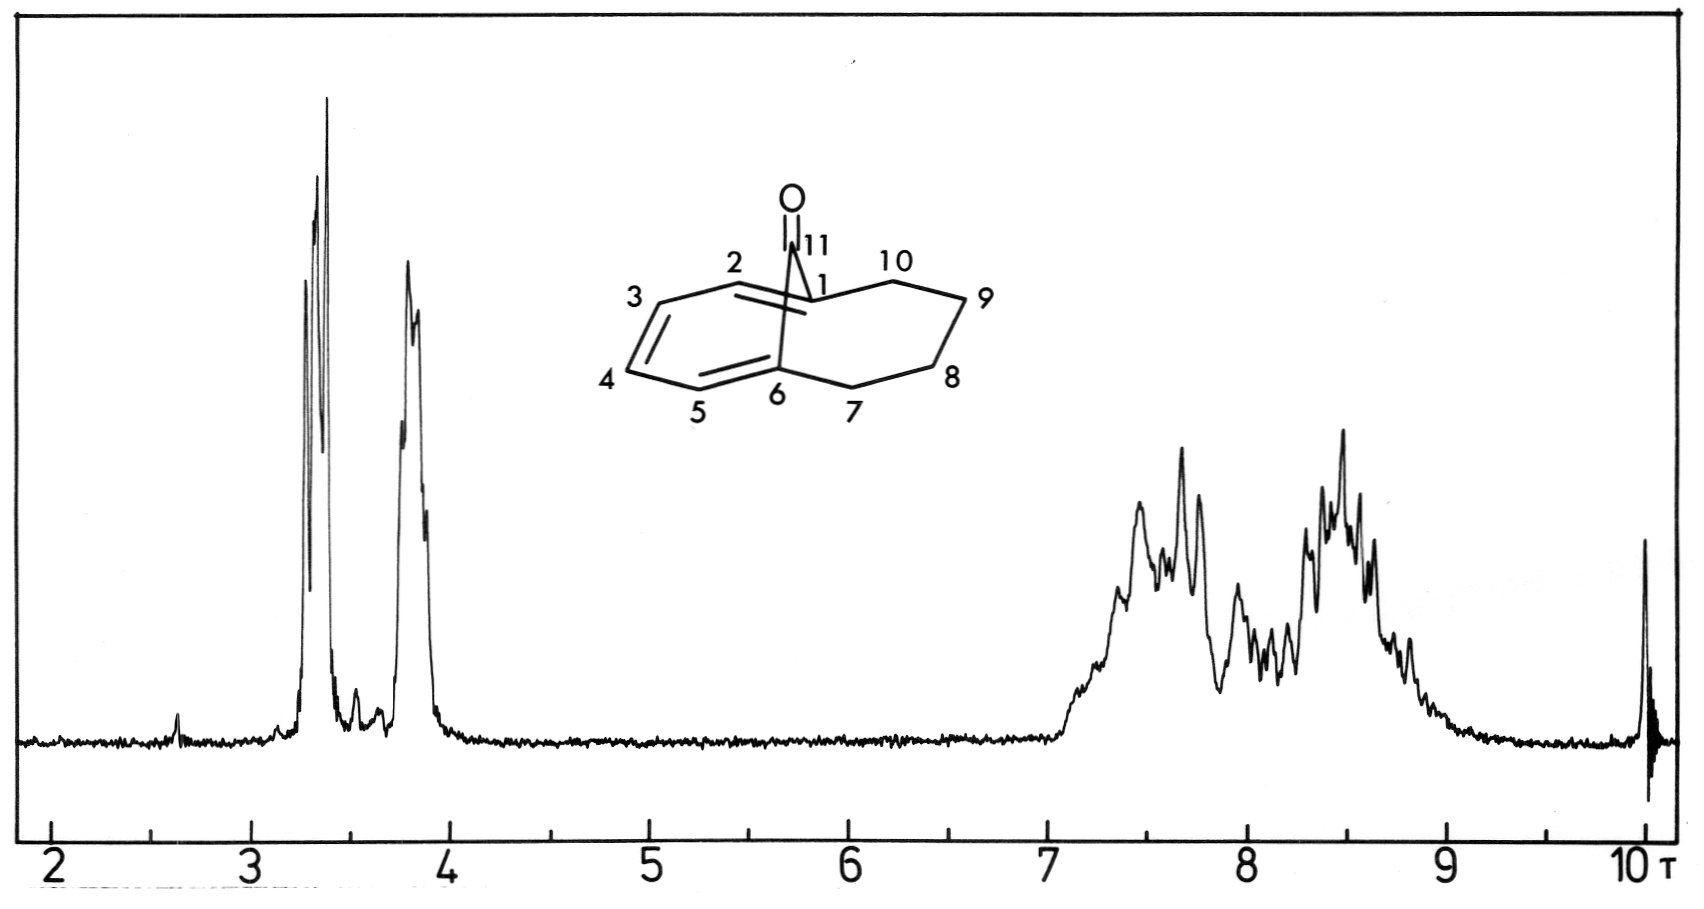
\includegraphics[width=14.427cm]{NMR_027}
\begin{alltt}
Abb. 27: \raise0.5ex\hbox{1}H-NMR-Spektrum des 11-Oxobicyclo[4.4.1]undecatriens-
(1,3,5) (13) in CDCl\lower0.5ex\hbox{3} (60 MHz; TMS als innerer Standard)

postulieren lässt, obwohl ohne Frage die Abwinkelung der Brücke
weiter besteht. Das in den \underline{endo}-Isomeren meist dreifach unterteilte
Multiplett der alicyclischen Protonen an C-7 - C-10 ist hier nur
einfach separiert und erscheint bei \(\tau\) = 7.05 - 9.17.

\end{alltt}
\hspace*{-0.25cm}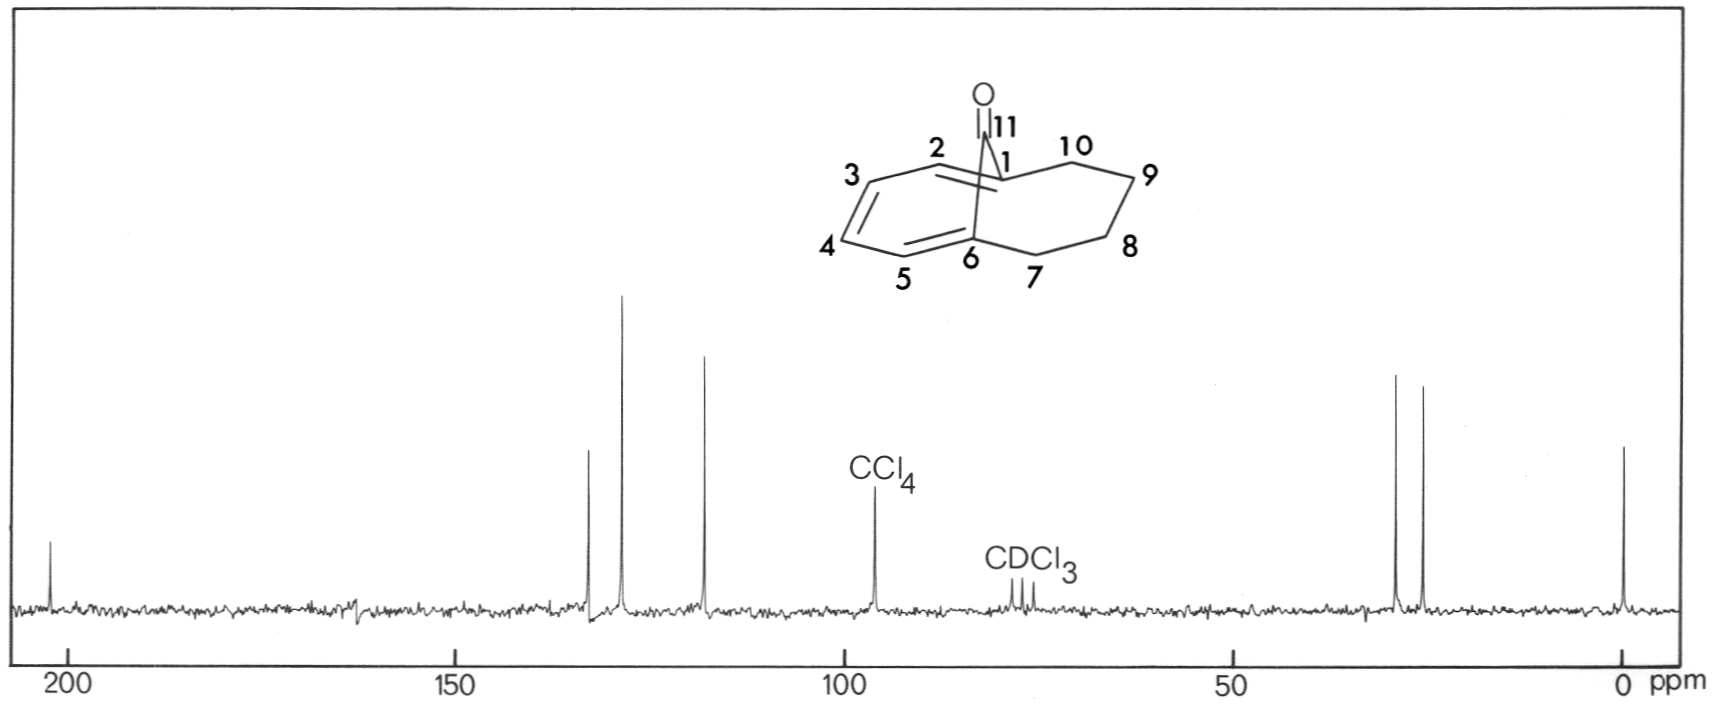
\includegraphics[width=14.52cm]{NMR_028}
\begin{alltt}
Abb. 28: \raise0.5ex\hbox{13}C-NMR-Spektrum des 11-Oxobicyclo[4.4.1]undeeatriens-
(1,3‚5) (13) in CCl\lower0.5ex\hbox{4}/CDCl\lower0.5ex\hbox{3} 3:1 (22.63 MHz; rauschent-
koppelt; TMS als innerer Standard; Lockfrequenz: \raise0.5ex\hbox{2}H-
Resonanz des CDCl\lower0.5ex\hbox{3})

 

\newpage
\makebox[0.8\textwidth][c]{- 60 -}


Mit 202.1 ppm tritt der Brückenkohlenstoff C-11 im \raise0.5ex\hbox{13}C-NMR-Spektrum
(s. Abb. 28 auF S. 59) an fast identischer Stelle wie im 11-Oxo-
bicyclo[4.4.1]undecatetraen-(1‚3,5,8) (14) in Resonanz. Auch die
übrigen wegen des Vorliegens einer Spiegelebene im Molekül auf fünf
reduzierten Signale für die Perimeterkohlenstoffe erscheinen mit
Ausnahme der Absorptionen für die Brückenbasisatome C-1 bzw. C-6
an den nach dem \raise0.5ex\hbox{13}C-NMR-Spektrum des "Tetreen-Ketons" (14) zu er-
wartenden Stellen (C-3,4: \(\delta\) = 128.7 ppm; C-2,5: \(\delta\) = 118.0 ppm;
C-7,10: \(\delta\) = 29.2 ppm; C-8‚9: \(\delta\) = 25.7 ppm). Die Tieffeldverschie-
bung von C-1,6 nach \(\delta\) = 133.0 ppm (\(\Delta\) = 7.4 ppm) lässt sich zwanglos
mit einer höheren sp\raise0.5ex\hbox{2}-Hybridisierung der Brückenbasis und dem damit
verbundenen höheren Abstand C1- C6 erklären. Überhaupt scheint die \raise0.5ex\hbox{13}C-
kernmagnetische Resonanz empfindlich auf eine zu- oder abneh-
mende Verdrillung der p\lower0.5ex\hbox{z}-Orbitale in diesen überbrückten Doppel-
bindungssystemen zu reagieren.

\end{alltt}
\begin{minipage}{10.5cm}
  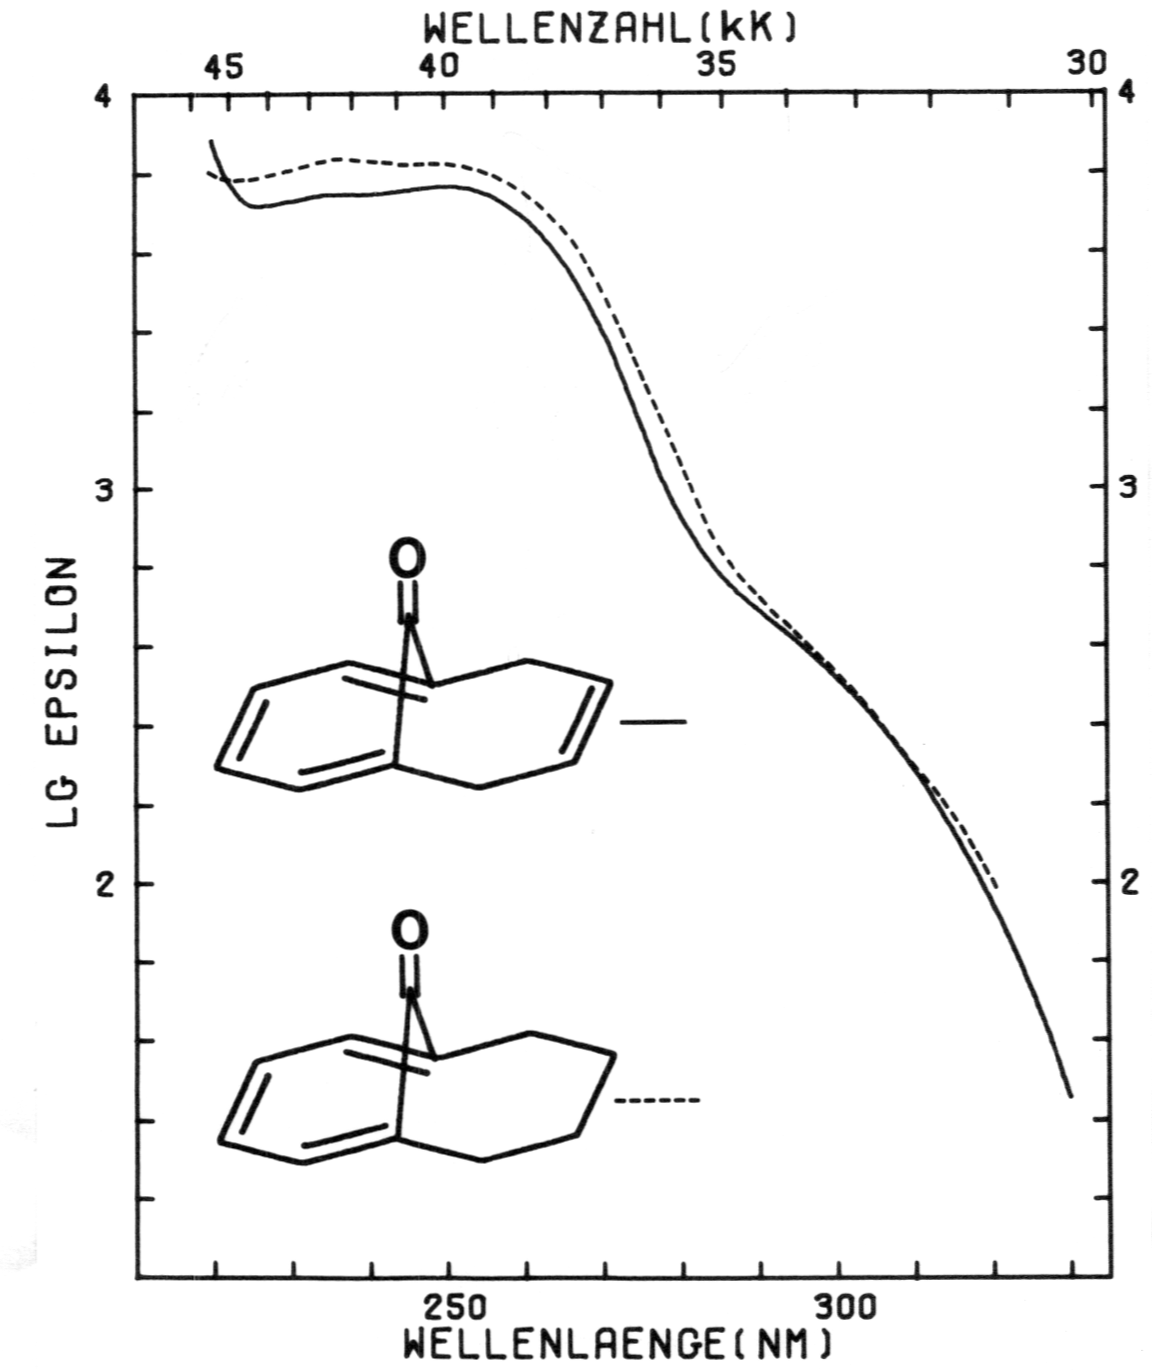
\includegraphics[width=9.75cm]{UV_029}
\end{minipage}%
%\hfill%
\begin{minipage}{0.3\textwidth}
\begin{alltt}
Abb. 29:
UV-Spektren des
11-Oxobicyclo-
[4.4.1]undecatetra-
ens-(1,3,5‚8) (14)
und des 11-Oxobicyclo-
[4.4.1]undecatriens-
(1,3,5) (13) in Cyclo-
hexan
\end{alltt}
\end{minipage}
\begin{alltt}
\newpage
\makebox[0.8\textwidth][c]{- 61 -}


Das Elektronenspektrum des 11-Oxobicyclo[4.4.1]undecatriens-(1‚3,5)
(13) ist mit zwei Maxima bei 237 und 247 nm Fast deckungsgleich
mit dem des 11-Oxobicyclo[4.4.1]undecatetraens-(1‚3,5,8) (14).
Wegen der höheren Extinktionswerte (\(\epsilon\) = 6800 bzw. 6600) dürfte in
diesem Molekül eine bessere Überlappung der \(\pi\)-Orbitale des Trien-
systems existieren.

2.4 Diskussion des troponoiden Charakters

Beim Vergleich der IR-Spektren von 2,7-disubstituierten Troponen
stellt man eine deutliche Diskrepanz in den Carbonylschwingungs-
frequenzen fest. Es fällt auf, daB die verbrückten Tropone, die
[n](2,7)-Troponophane (11), bei den niederen Gliedern der Reihe
höhere Werte für die Carbonylbande zeigen als die "offenen" Ver-
bindungen. Schließt man nämlich die Lücke zwischen der 2- und 7-
Stellung im Tropon (1) durch mehrere Methylengruppen (n\(\geq\)4), so
wird die vorherige Planarität des Tropongerüstes aufgehoben, da
das Molekül abhängig von der Größe der Brücke durch mehr oder
weniger große Abwinkelung der Carbonylgruppe der übergroßen Ring-
Spannung auszuweichen sucht, wobei jedoch der für eine sp\raise0.5ex\hbox{2}-Hybridi-
sierung an C-11 zu fordernde Winkel C1-C11-C6 erheblich verkleinert
und verbunden damit die IR-Frequenz \(\tilde{\nu}\)\lower0.5ex\hbox{C=O} erhöht wird (vgl. Tab. 4).
Infolge der dadurch gehinderten oder völlig unterbundenen Wechsel-
wirkung von Doppelbindungs- und Carbonylsystem gehen einige oder
alle der für Tropone typischen Eigenschaften verloren. So zeigt
das nonamethylenüberbrückte Tropon (11f) noch normale IR-Eigen-
schaften und wird in Trifluoressigsäure protoniert. Allerdings
weist das UV-Spektrum für das kurzwellige Maximum eine gegenüber
dem 2,7-Dimethyltropon (56) bereits erniedrigte Extinktion auf.
Bei den erstmals präparierten Ketonen (13), (14) und (15) ist die
Basizität überhaupt nicht mehr ausgeprägt, da eine Registrierung
der \raise0.5ex\hbox{1}H-NMR-Spektren in Trifluoressigsäure keinerlei Veränderung
zu den Aufnahmen in aprotischen Lösungsmitteln zeigt. Bei dem durch
Einführung eines Butadien-Segmentes in das Troponmolekül entstehen-
\newpage
\makebox[0.8\textwidth][c]{- 62 -}
\end{alltt}
\begin{table}[h!]\ttfamily
\captionsetup{singlelinecheck = false, justification=justified, labelfont=tt, textfont=tt}
\caption[caption]
    {\tabular[t]{@{}l@{}}C=O - Valenz- und C=C - Streckschwingungsfrequenzen im\\
    IR-Spektrum (in cm\raise0.5ex\hbox{-1}) sowie kurzwelliges Maximum (in nm)\\
    und Extinktion (in cm\raise0.5ex\hbox{2}·mol\raise0.5ex\hbox{-1}) im Elektronenspektrum eini-\\
    ger 2‚7-dialkylsubstituierter Tropone\endtabular}
\label{tab:IRKetonDaten}
 \begin{tabular}{cccclc}
 \  & \  & $\tilde{\nu}$\lower0.5ex\hbox{C=O} & $\tilde{\nu}$\lower0.5ex\hbox{C=C} &%
  $\ \lambda$\lower0.5ex\hbox{max}\quad ($\epsilon$)\   & Liter.\\[0.5ex]
% 2,7-Dimethyltropon (56)
\chemfig[atom style={scale=0.8}]{*7(-=(-CH_3)-(=[,0.7]O)-(-CH_3)=-=)}%
\cmpd*{dimethyltropon}%
 & (56) & 1620 & \specialcell{1600\\[-0.5ex]1570} & 234 (\,30500\,) &  [107]\\[24pt]
% 2,7-Diisopropyltropon (57)
\chemfig[atom style={scale=0.8}]{*7(-=(-[,0.8](-[::45,0.8])(-[::-45,0.8]))-(=[,0.7]O)-(-[,0.8](-[::45,0.8])(-[::-45,0.8]))=-=)}%
\cmpd*{diisopropyltropon}%
 & (57) & \  & 1571 & 238 (\,17800\,) & [108]\\[24pt]
% 2,7-Di-tert.-butyltropon (58)
\chemfig[atom style={scale=0.8}]{*7(-=(-[,0.8](-[::-90,0.8])(-[::90,0.8])(-[::0,0.8]))-(=[,0.7]O)-(-[,0.8](-[::90,0.8])(-[::-90,0.8])(-[::0,0.8]))=-=)}%
\cmpd*{ditbutyltropon}%
 & (58) & 1635 & \specialcell{1610\\[-0.5ex]1590} & 237 (\,15000) &  [107]\\[24pt]
\schemestart
\pgfmathsetmacro{\currentscale}{0.9}%
% drawn clockwise from bridge atom
\chemfig[atom style={scale=0.9}]{?@{u}=_[:-168,,,,shrtdbl={1pt}{2pt}]-[:168]=_[:60,,,,shrtdbl={0pt}{3.5pt}]-[:12]=_[:-12]%
(@{o}-[:-252]?(=[:90,0.6]O)% bridge 1-6
(-[:-30,2.75,,,draw=none]{(}@{n}CH_2{)}_9))% varable CH2 groups
}%
\chemmove{\draw[thick,-](o).. controls +(30:0.75cm) and +(120:0.75cm).. (n);}%
\chemmove{\draw[thick,-](u).. controls +(-30:0.75cm) and +(-120:0.75cm).. (n);}%
\schemestop%
 & (11f) & 1620 & 1575 & 239 (\,20400\,) &  [33]\\[16pt]
\schemestart
% drawn clockwise from bridge atom
\chemfig[atom style={scale=0.9}]{?@{u}=_[:-168,,,,shrtdbl={1pt}{2pt}]-[:168]=_[:60,,,,shrtdbl={0pt}{3.5pt}]-[:12]=_[:-12]%
(@{o}-[:-252]?(=[:90,0.6]O)% bridge 1-6
(-[:-30,2.75,,,draw=none]{(}@{n}CH_2{)}_6))% varable CH2 groups
}%
\chemmove{\draw[thick,-](o).. controls +(30:0.75cm) and +(120:0.75cm).. (n);}%
\chemmove{\draw[thick,-](u).. controls +(-30:0.75cm) and +(-120:0.75cm).. (n);}%
\schemestop%
 & (11c) & 1656 & \  & \  & [32]\\[16pt]
\schemestart
% drawn clockwise from bridge atom
\chemfig[atom style={scale=0.9}]{?@{u}=_[:-168,,,,shrtdbl={1pt}{2pt}]-[:168]=_[:60,,,,shrtdbl={0pt}{3.5pt}]-[:12]=_[:-12]%
(@{o}-[:-252]?(=[:90,0.6]O)% bridge 1-6
(-[:-30,2.75,,,draw=none]{(}@{n}CH_2{)}_4))% varable CH2 groups
}%
\chemmove{\draw[thick,-](o).. controls +(30:0.75cm) and +(120:0.75cm).. (n);}%
\chemmove{\draw[thick,-](u).. controls +(-30:0.75cm) and +(-120:0.75cm).. (n);}%
\schemestop%
 & (11a) & 1729 & 1602 & 237 (\,6800\,) & [d.A.]\\[16pt]
 % 11-Oxo-1,6-methano-undecatetraen (14)
\chemfig[atom style={scale=0.9}]{=_[:60,,,,shrtdbl={0pt}{3.5pt}]-[:12]=_[:-12]%
(-[:-252]?(=[:90,0.6]O))% 1,6 Brücke
-[:12]-[:-12]=_[:-120,,,,shrtdbl={0pt}{3.5pt}]-[:-168]-[:168]?=_[:-168,,,,shrtdbl={1pt}{2pt}]-[:168]}%
 & (14) & 1740 & \specialcell{1632\\[-0.5ex]1598} & 235 (\,5600\,) & [d.A.]\\[16pt]
 % 11-Oxo-1,6-methano-[10]annulen (15)
\chemfig[atom style={scale=0.9}]{=_[:60,,,,shrtdbl={0pt}{3.5pt}]-[:12]=_[:-12]%
(-[:-252]?(=[:90,0.6]O))% 1,6 Brücke
-[:12]=_[:-12,,,,shrtdbl={4pt}{0pt}]-[:-120]=_[:-168]-[:168]?=_[:-168,,,,shrtdbl={1pt}{2pt}]-[:168]}%
 & (15) & 1740 & \  & 252 (\,74000\,) & [d.A.]%
% reset scale to normal
\pgfmathsetmacro{\currentscale}{\normalscale}%
 \end{tabular}
\end{table}
\begin{alltt}
den Keton (15) handelt es sich darüber hinaus laut UV-Spektrum um
einen typischen Vertreter der [10]Annulenreihe‚ der weder die für
Tropone noch für Ketone typischen Reaktionsmechanismen zeigt. Die
beiden anderen Ketone (13) und (14) verhalten sich dem gegenüber
\newpage
\makebox[0.8\textwidth][c]{- 63 -}


wie sterisch gehinderte aliphatische Ketone, die sich z.B. in die
Ketale umwandeln lassen. Die geringen Extinktionswerte der kurz-
welligen Bande im UV-Spektrum sprechen weiterhin dafür, daß die
Konjugation zwischen dem Carbonylchromophor und dem Doppelbindungs-
system zusammengebrochen ist; es liegt nur ein mäßig konjugiertes
Trien vor. Durch eine Tetramethylenbrücke wird die troponoide
Struktur somit völlig zerstört, so daß die Verbindungen (13) und
(14) nur unter Vorbehalt als [4](2,7)-Troponophane bezeichnet
werden dürfen; für das 11-Oxo-1,6-methano-[10Jannulen (15) ist
dieser Ausdruck unangebracht.

2.5 11-Oxo-1,2-benzo-4‚9-methano-[10]annulen (61) \raise0.5ex\hbox{[109a]} \leavevmode\raise0.5ex\hbox{*})

Die kürzlich gelungene Synthese des 1‚2-Benzo-4,9-methano-[10]annu-
lens (62) \raise0.5ex\hbox{[109b]} lenkte die Aufmerksamkeit auf das entsprechende
Ketoderivat (61).

\end{alltt}
\schemestart[]
\hspace{0.5cm}
% Vorabdefinitionen
% Tropon-Butadien-Addukt (59)
\cmpd*{troponbutadienaddukt}
% Nummer 60 (bis jetzt nicht gefunden)
\cmpd*{nummer60}
% Benzo-11-oxo-1,6-methano-[10]annulen (61)
\chemname[18pt]{
\chemfig{-[:60]=_[:12]-[:-12]%
(-[:-252]?(=[:90,0.6]O))% 1,6 Bruecke
=_[:12]-[:-12](-[:12]=_[:-12,,,,shrtdbl={3.5pt}{0pt}]-[:-120]%
=_[:-168]-[:168])=_[:-120,,,,shrtdbl={0pt}{3.5pt}]-[:-168]=_[:168,,,,shrtdbl={3pt}{0pt}]?%
-[:-168]=_[:168,,,,shrtdbl={3.5pt}{0pt}]}%
}{\cmpd{benzohexaentroponophan}}%
% invisible shortened arrow to separate compounds and align them
\arrow(.mid east--.mid west){0}[,.4]
% Benzo-1,6-methano-[10]annulen (62)
\chemname[18pt]{
\chemfig{-[:60]@{n7}%
=_[:12]@{n8}%
-[:-12]@{n9}%
(-[:-252]?@{n11})% 1,6 Brücke
=_[:12]@{n10}%
-[:-12]@{n1}%
(-[:12]@{n66}%
=_[:-12,,,,shrtdbl={3.5pt}{0pt}]@{n55}%
-[:-120]@{n44}%
=_[:-168]@{n33}%
-[:168])%
=_[:-120,,,,shrtdbl={0pt}{3.5pt}]@{n2}%
-[:-168]@{n3}%
=_[:168,,,,shrtdbl={3pt}{0pt}]?@{n4}%%
-[:-168]@{n5}%%
=_[:168,,,,shrtdbl={3.5pt}{0pt}]@{n6}%
}%
\chemmove{% with scale=1.0
    \node at (n1) [above=0.08] {\scriptsize\textsf{1}};
    \node at (n2) [below=0.08] {\scriptsize\textsf{2}};
    \node at (n3) [below=0.08] {\scriptsize\textsf{3}};
    \node at (n4) [below=0.08] {\scriptsize\textsf{4}};
    \node at (n5) [below=0.08] {\scriptsize\textsf{5}};
    \node at (n6) [left=0.06] {\scriptsize\textsf{6}};
    \node at (n7) [left=0.08] {\scriptsize\textsf{7}};
    \node at (n8) [above=0.08] {\scriptsize\textsf{8}};
    \node at (n9) [above right=0.08 and 0.04] {\scriptsize\textsf{9}};
    \node at (n10) [above=0.08] {\scriptsize\textsf{10}};
    \node at (n11) [right=0.08] {\scriptsize\textsf{11}};
    \node at (n33) [below=0.08] {\scriptsize\textsf{3'}};
    \node at (n44) [right=0.12] {\scriptsize\textsf{4'}};
    \node at (n55) [right=0.08] {\scriptsize\textsf{5'}};
    \node at (n66) [above=0.08] {\scriptsize\textsf{6'}};
}%
}{\cmpd{benzomethano10annulen}}
\schemestop
\chemnameinit{}
\begin{alltt}

Von seiner Darstellung konnte man weitere klärende Aspekte zum
Phänomen der Benzoannelierung \raise0.5ex\hbox{[110]} erwarten. Anneliert man nämlich
einem Annulen mit delokalisiertem \(\pi\)-Elektronensystem einen Benzol-
ring, so sollte die Delokalisation in einem Ringteil aufgehoben
werden. Infolge der höheren Stabilität des Elektronensextetts im
Benzolkern ist somit eine merkliche Bindungsfixierung im Annulenteil
vorherzusagen. Dieser Effekt wird auch allgemein beobachtet \raise0.5ex\hbox{[111]}
und tritt ebenfalls - \raise0.5ex\hbox{1}H-NMR-spektroskopisch nachweisbar - im
1,2-Benzo-4‚9-methano-[10Jannulen (62) auf. Analog zum nicht anne-
lierten aromatischen Keton (15) sollte die entsprechende Benzoverbin-

\(\overline{\hspace{7cm}}\)
\leavevmode\raise0.5ex\hbox{*}) Die Bezifferung der Kohlenstoffatome erfolgte nach der IUPAC-
   Regel Nummer A 23.5 von 1957 \raise0.5ex\hbox{[113]}.

\newpage
\makebox[0.8\textwidth][c]{- 64 -}


dung (61) stärker eingeebnet sein und dadurch eine höhere Elek-
tronendelokalisation bedingen, so daß der Einfluss der Annelierung
zumindest geschwächt würde. A priori ist auch eine Störung des
Benzolsystems selbst nicht auszuschließen.

\end{alltt}
\schemestart
\hspace{3cm}
% Benzo-11-bromo-1,6-methano-[10]annulen (63)
\chemname{
\chemfig{-[:60]=_[:12]-[:-12]%
(-[:-252]?(-[:15]Br))% 1,6 Bruecke
=_[:12]-[:-12](-[:12]=_[:-12]-[:-120]=_[:-168]-[:168])=_[:-120]-[:-168]=_[:168]?-[:-168]=_[:168]}%
}{\cmpd{brombenzomethano10annulen}}
\schemestop
\chemnameinit{}
\begin{alltt}

Nach dem bewährten Syntheseprinzip müsste eine Präparierung des
11-Oxo-1,2-benzo-4,9-methano-[10]annulens (61) vom 11-Brom-1,2-
benzo-4,9-methano-[10]annulen (63) ausgehen, das jedoch in einer
vielstufigen Reaktionsfolge nur in einer Gesamtausbeute von 0.05 \%
(bezogen auf 1,4,5,8,9,10-Hexahydroanthracen) zugänglich ist.

Während der Durchführung dieser Arbeit wurde von S. Ito et al. \raise0.5ex\hbox{[112]}
ein alternativer Weg zum 11-Oxo-1,6-methano-[10]annulen (15) pub-
liziert. Die Autoren fanden, daß Tropon (1) thermisch 1,3-Butadien
im Sinne einer [6 + 4]-Cycloaddition addiert.

\end{alltt}
\schemestart
\hspace{0.5cm}
% Tropon-Butadien-Addition
\chemname{
\chemfig{=_[@{p5a}:60]-[@{p1e}:12]=_[@{p1a}:-12]%
(-[:-252]?(=[:90,0.6]O))% 1,6 Brücke
-[@{p2e}:12,,,,draw=none]=_[@{p2a}:-12]-[@{p3e}:-120]=_[@{p3a}:-168]%
-[@{p4e}:168,,,,draw=none]?=_[@{p4a}:-168]-[@{p5e}:168]}%
}{\cmpd{tropon}}
\chemmove{
\draw[shorten <= 3pt](p1a)..controls +(-135:5mm) and +(-45:5mm)..(p1e);
\draw[shorten <= 3pt](p2a)..controls +(-135:5mm) and +(-45:5mm)..(p2e);
\draw[shorten <= 3pt](p3a)..controls +(135:5mm) and +(174:5mm)..(p3e);
\draw[shorten <= 3pt](p4a)..controls +(81:5mm) and +(108:5mm)..(p4e);
\draw[shorten <= 3pt](p5a)..controls +(6:5mm) and +(45:5mm)..(p5e);
}
\arrow(.mid east--.mid west){->[\textsf{$\Delta$T}]}
% Tropon-Butadien-Addukt (59)
\chemname{
\chemfig{-[:60]=_[:12]-[:-12]%
(-[:-252]?(=[:90,0.6]O))% 1,6 Bruecke
-[:12]-[:-12]=_[:-120]-[:-168]-[:168]?-[:-168]=_[:168]}%
}{\cmpd{troponbutadienaddukt}}
\arrow(.mid east--.mid west){->[\textsf{DDCh}]}
% 11-Oxo-1,6-methano-[10]annulen (15)
\chemname{
\chemfig{=_[:60]-[:12]=_[:-12]%
(-[:-252]?(=[:90,0.6]O))% 1,6 Brücke
-[:12]=_[:-12]-[:-120]=_[:-168]-[:168]?=_[:-168]-[:168]}%
}{\cmpd{hexaentroponophan}}%
\schemestop
\chemnameinit{}
\begin{alltt}

Das gebildete 11-Oxobicyclo[4.4.1]undecatrien-(2‚4,8) (59) kann in
geringer Ausbeute (unter 10 \% d.Th.) in das aromatische Keton (15)
durch Dehydrierung mit DDCh überführt werden. Die Synthese kann nur
wegen der Kürze der Reaktionsschritte als effizient bezeichnet wer-
den, da die Gesamtausbeute (7 \% d.Th. bezogen auf Tropon) nur un-
wesentlich höher liegt als die auf konventionellem Wege - allerdings
über sieben Stufen - erzielte Ausbeute (5 \% d.Th. bezogen auf Naph-
thalin). Übertragung dieses Schemas auf die Darstellung des 11-Oxo-
1,2-benzo-4,9-methano-[10]annulens (61) bedeutet Addition eines
Sechsringes mit zwei vicinalen, exocyclischen Methylengruppen an
Tropon (1). Hierfür käme insbesondere o-Xylylen infrage.

\newpage
\makebox[0.8\textwidth][c]{- 65 -}


2.5.1 11-Oxo-3',6'‚3,4,9,10-hexahydro-1,2-benzo-4,9-methano-
      [10]annulen (64)

Statt o-Xylylen stand durch Synthesevorhaben des hiesigen Arbeits-
kreises \raise0.5ex\hbox{[109b,122]} das gleichermaßen geeignete 1‚6-Dimethylen-
cyclohexen-3 (66) zur Verfügung, das in vierfachem ÜberschuB bei
120\degree{}C mit Tropon (1) zur Reaktion gebracht wurde. Nach Säulen-
chromatographie an Kieselgel (Eluens: Methylenchlorid) fallen
neben dem Dimeren des 1‚6-Dimethylencyclohexens-3 als zweite Frak-
tion farblose Kristalle vom Fp = 41 - 42.5\degree{}C an.

\end{alltt}
\schemestart
\hspace{0.75cm}
% Vorabdefinitionen
% Tropon-Dimethylencyclohexen-Addukt (64)
\cmpd*{tropondimethylencyclohexenaddukt}
% Benzo-Tropon-Butadien-Addukt (65)
\cmpd*{benzotroponbutadienaddukt}
% Tropon (1) und 1,6-Dimethylen-cyclohexen-3 (66)
\chemname{
\chemfig{=_[:60]-[:12]=_[:-12]%
(-[:-252]?(=[:90,0.6]O))% 1,6 Brücke
-[:12,,,,draw=none]=_[:-12](-[:12]-[:-12]=_[:-120]-[:-168]-[:168])-[:-120]=_[:-168]-[:168,,,,draw=none]?=_[:-168]-[:168]}%
}{\cmpd{tropon dimethylencyclohexen}}%
\arrow(.mid east--.mid west){->[\textsf{$\Delta$T}]}%
% Tropon-Dimethylencyclohexen-Addukt (64)
\chemname{%
\chemfig{-[:60]=_[:12]-[:-12]%
(-[:-252]?(=[:90,0.6]O))% 1,6 Bruecke
-[:12]-[:-12](-[:12]-[:-12]=_[:-120]-[:-168]-[:168])=_[:-120]-[:-168]-[:168]?-[:-168]=_[:168]}%
}{\cmpd{tropondimethylencyclohexenaddukt}}
\schemestop
\chemnameinit{}
\begin{alltt}

Die Molekülstruktur entspricht nach Elementaranalyse und IR-Spek-
trum (intensive Bande bei \(\tilde{\nu}\)\lower0.5ex\hbox{C=O} = 1702 cm\raise0.5ex\hbox{-1}) der eines Ketons.

Das \raise0.5ex\hbox{1}H-NMR-Spektrum (s. Abb. 30 auf S. 66) erlaubt eine eindeutige
Identifizierung der Verbindung. Die charakteristischen Signale für
das konjugierte Diensystem bei \(\tau\) = 3.95 - 4.73 und die tertiären
Protonen an C-4 bzw. C-9 (Pseudoquartett bei \(\tau\) = 6.50) entsprechen
genau dem Spektrum des nicht annelierten Ketons (59). Weiterhin
erscheinen die olefinischen Protonen H-4' bzw. H-5' erwartungsge-
mäß als Singulett bei \(\tau\) = 4.39, während die zugehörigen Allyle des
1,4-dihydrierten Benzolringes bei \(\tau\) = 7.37 absorbieren. Die rest-
lichen Protonen geben ein zunächst nicht deutbares Multiplett, des-
sen Habitus sich jedoch mit Hilfe der Verschiebungs-Reagens-
Technik \raise0.5ex\hbox{[113]} klären ließ. Dabei werden der Probenlösung paramag-
netische Seltenerdchelate als "Shiftreagentien" zugesetzt, die zwei
unbesetzte Koordinationslücken durch Komplexierung mit einsamen
Elektronenpaaren von funktionellen Gruppen des Moleküls aufzufüllen
vermögen. In einem derartigen Komplex herrscht zusätzlich zum äus-
seren angelegten Magnetfeld ein durch den Paramagnetismus des
Chelations hervorgerufenes konstantes Feld, dessen Einfluss auf die
einzelnen Protonen von deren Entfernung und Winkel zum Zentralion

\newpage
\makebox[0.8\textwidth][c]{- 66 -}


\end{alltt}
\hspace*{-0.25cm}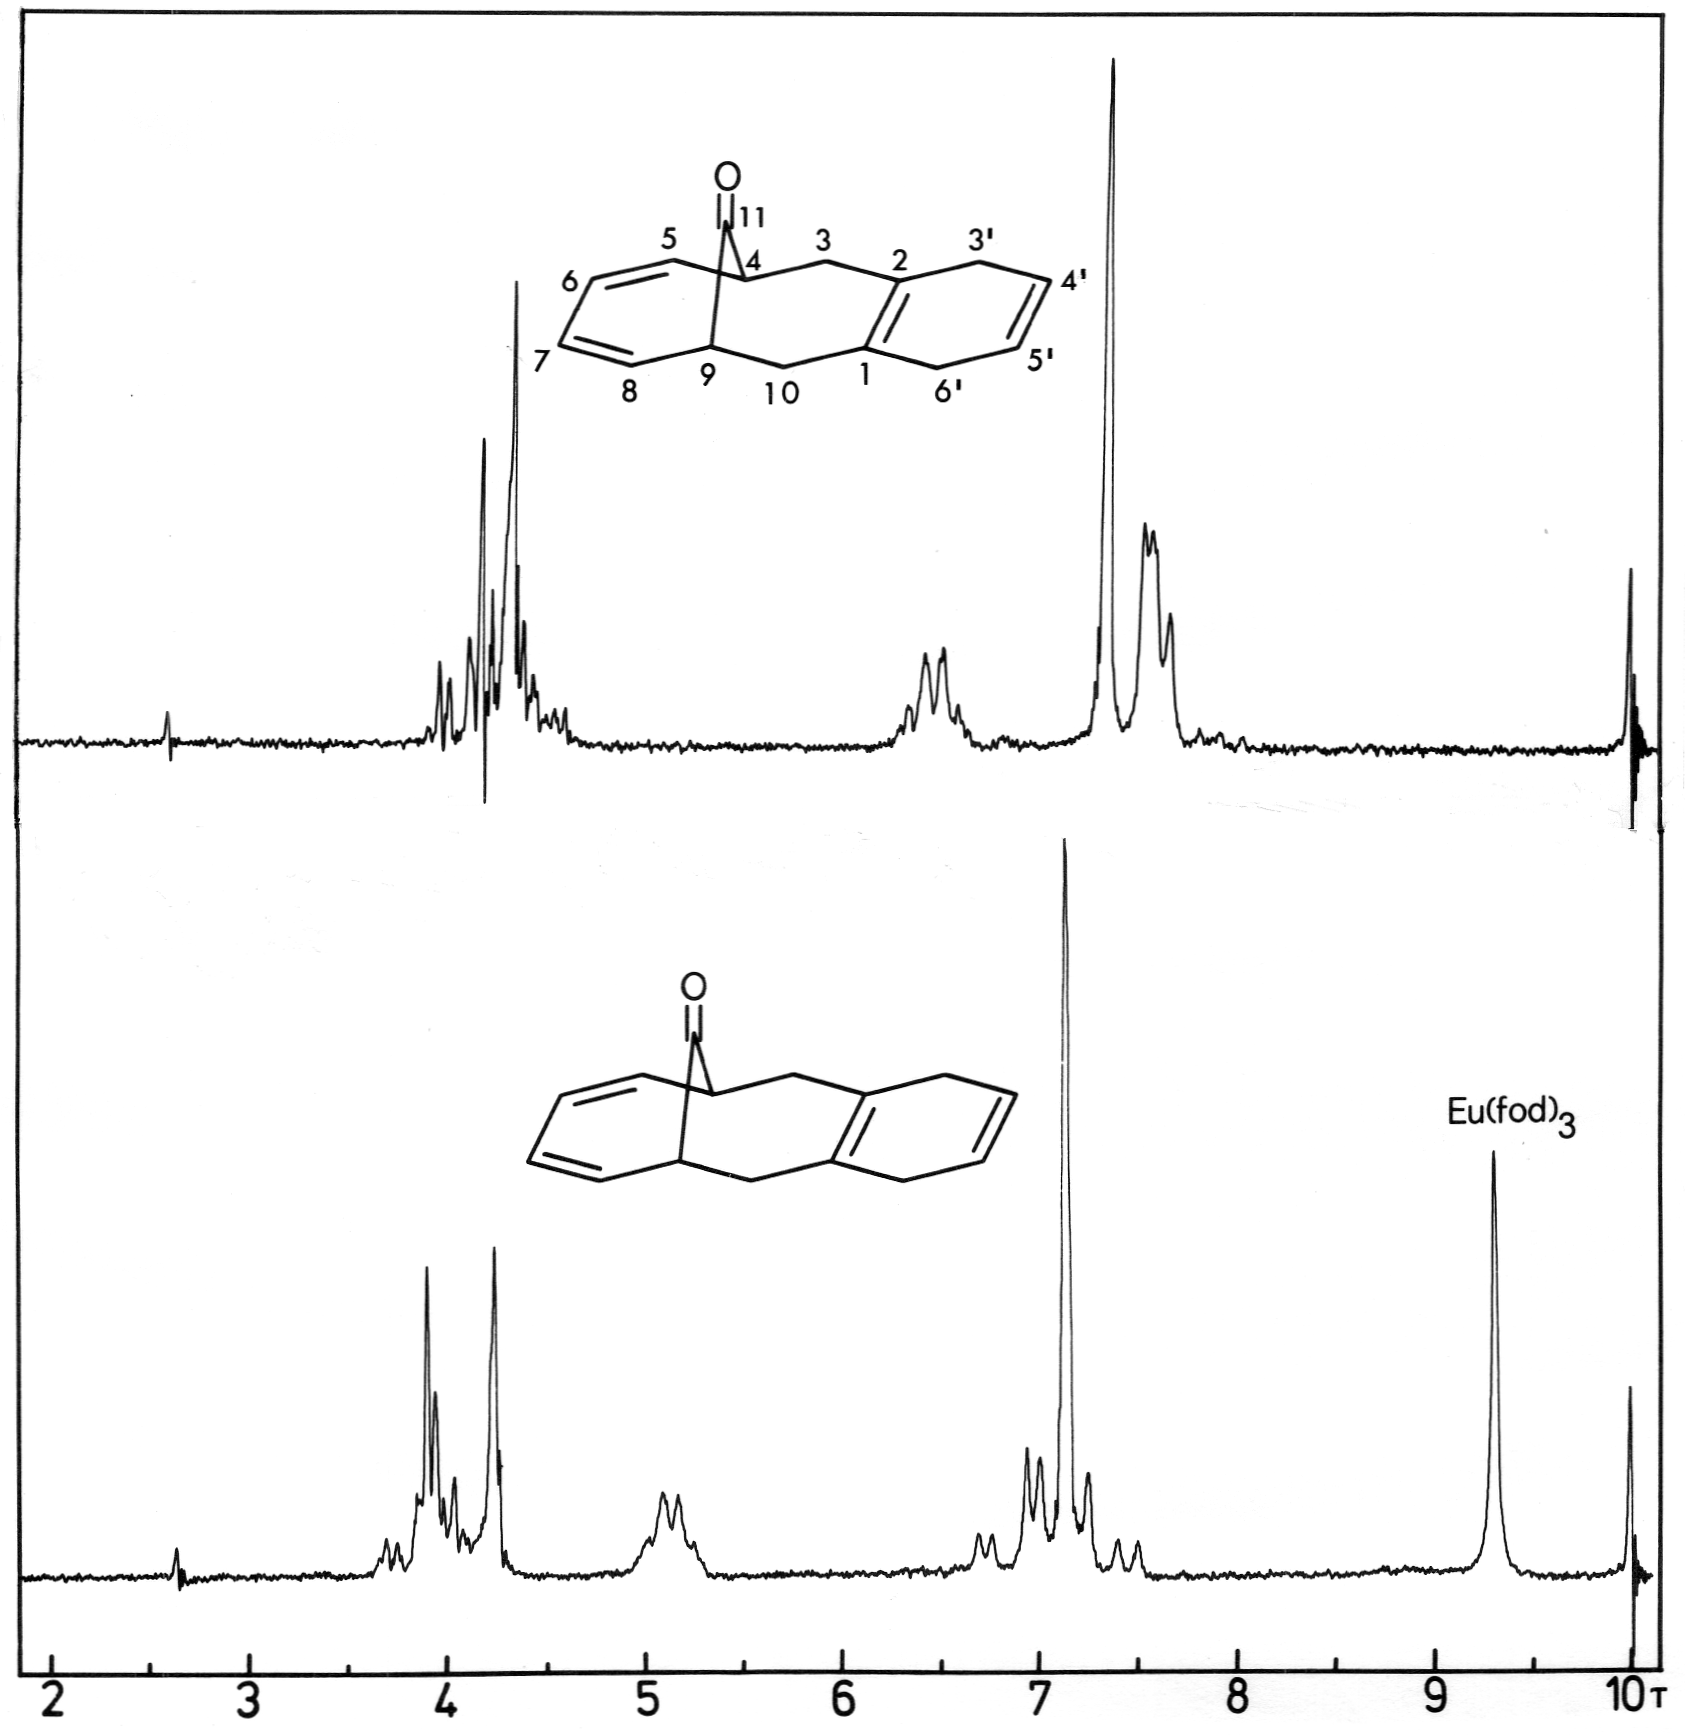
\includegraphics[width=14.27cm]{NMR_030}
\begin{alltt}
Abb. 30: \raise0.5ex\hbox{1}H-NMR-Spektrum des 11-Oxo-3',6',3‚4‚9,10-hexahydro-1‚2-
benzo-4,9-methano-[10]annulens (64) in CDCl\lower0.5ex\hbox{3}, einmal ohne
und einmal mit Zusatz von Tris-1‚1‚1,2‚2,3,3-heptafluor-
7,7-dimethyloctadionato-(4,6)-europium (60 MHz; TMS als
innerer Standard)

abhängt. Die dadurch bedingte unterschiedliche Verschiebung erlaubt
oft eine Analyse des Spektrums nach erster Ordnung. Bei Verwendung
von Tris-1‚1‚1‚2,2‚3,3-heptafluor-7,7-dimethyloctadionato-(4,6)-
europium resultiert eine Verschiebung nach tieferem Feld, so daß
die Nachbarschaft der Protonen H-4 bzw. H-9 zur Carbonylgruppe zwang-
los aus ihrer hohen Shiftrate folgt. Auch das Multiplett des Dien-
systems ist jetzt deutlich vom Singulett der olefinischen Protonen

\newpage
\makebox[0.8\textwidth][c]{- 67 -}


H-4' bzw. H-5' separiert. Das Multiplett schließlich für die
allylischen Protonen an C-3 bzw. C-10 besteht aus zwei überla-
gerten AB-Systemen mit der Kopplungskonstante J\lower0.5ex\hbox{AB} = 14.5 Hz.



2.5.2 11-Oxo-3,4,9,10-tetrahydro-1‚2-benzo-4,9-methano-
[10]annulen (65)
 

Bereits bei Raumtemperatur wird das 1‚4-Cyclohexadien-Segment des
11-Oxo-3',6',3,4,9‚10-hexahydro-1,2-benzo-4,9-methano-[10]annulens
(64) bei Zugabe von DDCh dehydriert - erkenntlich am sofortigen
Ausfall des zugehörigen Hydrochinons. Nach "Filtration" über eine
kurze Säule (Aluminiumoxid; Eluens: Methylenchlorid) erhält man
in praktisch quantitativer Ausbeute weiße Kristalle vom Fp = 74 -
75\degree{}C.

\end{alltt}
\schemestart
\hspace{0.75cm}
% Tropon-Dimethylencyclohexen-Addukt (64)
\chemname{
\chemfig{-[:60]=_[:12]-[:-12]%
(-[:-252]?(=[:90,0.6]O))% 1,6 Bruecke
-[:12]-[:-12](-[:12]-[:-12]=_[:-120]-[:-168]-[:168])=_[:-120]-[:-168]-[:168]?-[:-168]=_[:168]}%
}{\cmpd{tropondimethylencyclohexenaddukt}}
\arrow(.mid east--.mid west){->[\textsf{DDCh}][\textsf{RT}]}
% Benzo-Tropon-Butadien-Addukt (65)
\chemname{
\chemfig{-[:60]=_[:12]-[:-12]%
(-[:-252]?(=[:90,0.6]O))% 1,6 Bruecke
-[:12]-[:-12](-[:12]=_[:-12]-[:-120]=_[:-168]-[:168])=_[:-120]-[:-168]-[:168]?-[:-168]=_[:168]}%
}{\cmpd{benzotroponbutadienaddukt}}
\schemestop
\chemnameinit{}
\begin{alltt}

Die Carbonylgruppe dokumentiert sich unverändert deutlich im IR-
Spektrum durch die starke Bande bei 1690 cm\raise0.5ex\hbox{-1}, während sich das
typische Muster der Out-of-Plane-Schwingungen des ortho-disubstitu-
ierten Benzolringes bei 750 cm\raise0.5ex\hbox{-1} identifizieren lässt.

Das \raise0.5ex\hbox{1}H-NMR-Spektrum präsentiert sich fast völlig unverändert. Als
neue Signalgruppe tritt ein enges AA'BB'-System für die Benzol-
protonen zentriert bei \(\tau\) = 2.94 in Erscheinung, was einen Reaktions-
ablauf in der gewünschten Weise wahrscheinlich macht. Zusatz von
Eu(fod)\lower0.5ex\hbox{3} zu der Probe erlaubt die Bestimmung der Kopplungskonstante
der beiden überlagerten AB-Systeme bei \(\tau\) = 6.65 - 7.25 zu J\lower0.5ex\hbox{AB} =
14.5 Hz, so daß die Ähnlichkeit der Verbindung mit dem Keton (64)
als gesichert gelten darf.

\newpage
\makebox[0.8\textwidth][c]{- 68 -}



\end{alltt}
\hspace*{-0.2cm}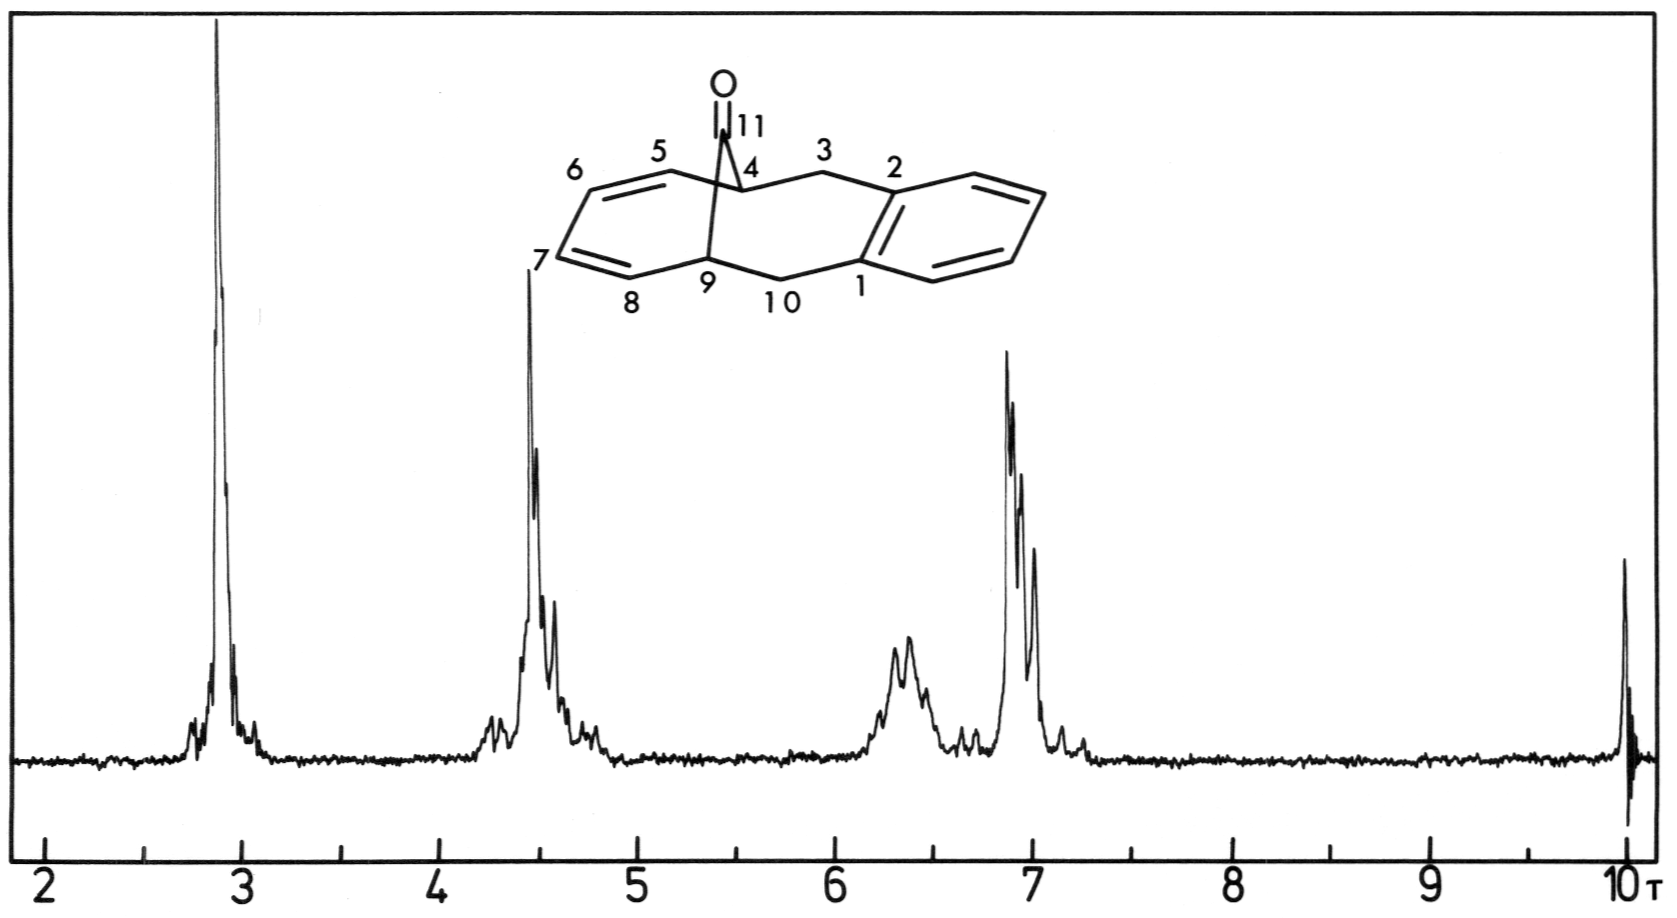
\includegraphics[width=14.22cm]{NMR_031}
\begin{alltt}
Abb. 31: \raise0.5ex\hbox{1}H-NMR-Spektrum des 11-Oxo-3,4,9,10-tetrahydro-1,2-benzo-
         4,9-methano-[10]annulens (66) in CDCl\lower0.5ex\hbox{3} (60 MHz; TMS als
         innerer Standard.


\end{alltt}
\begin{minipage}{10.0cm}
  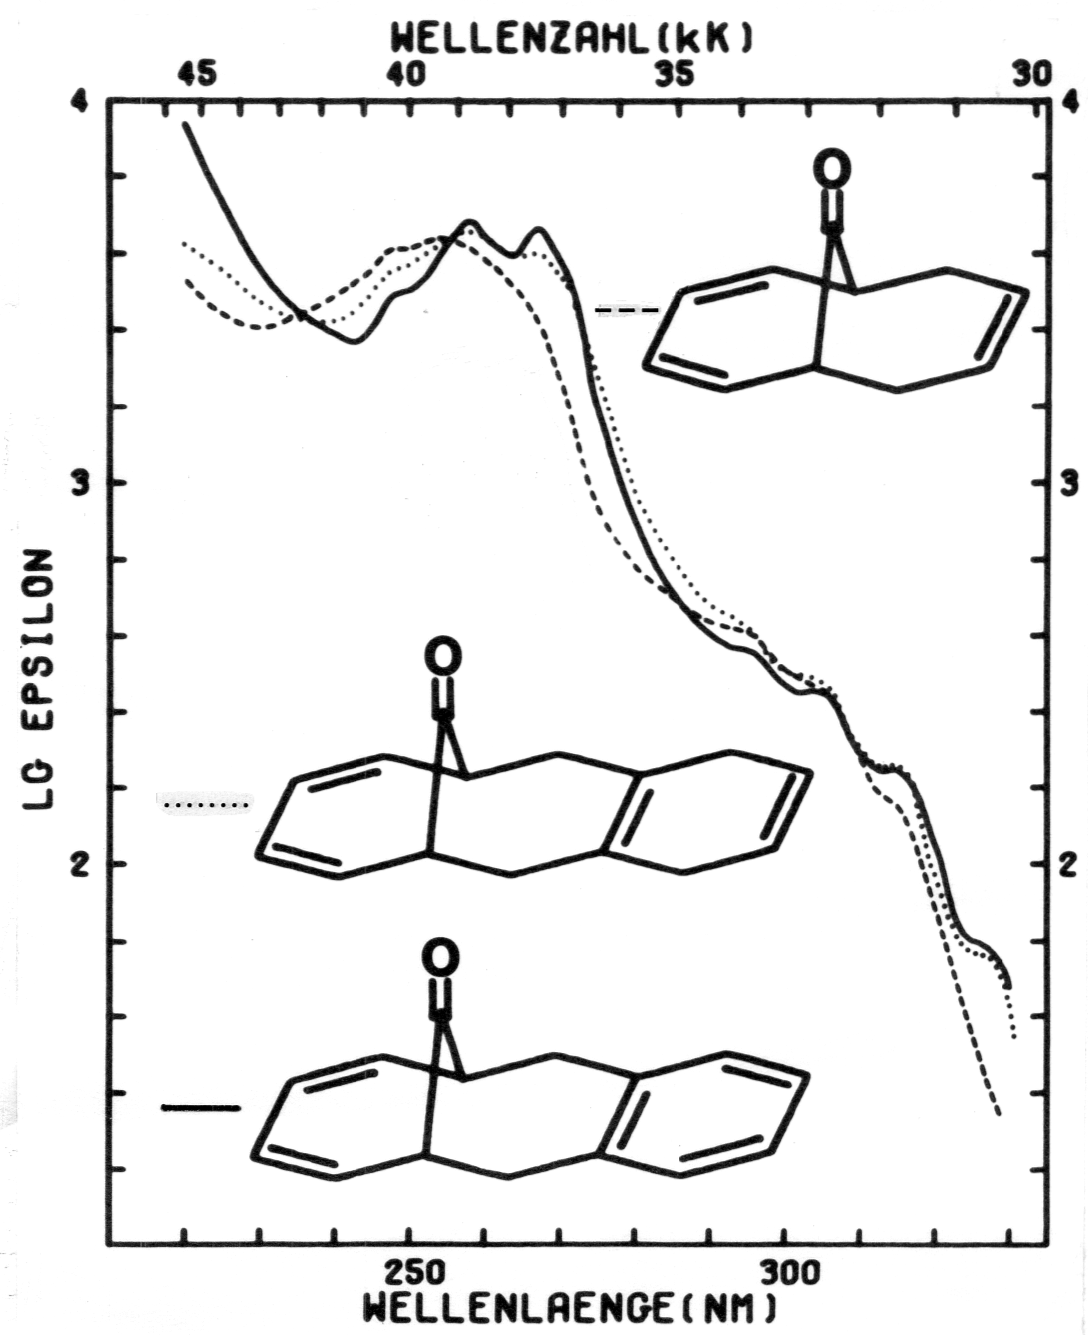
\includegraphics[width=9.21cm]{UV_032}
\end{minipage}%
%\hfill%
\begin{minipage}{0.4\textwidth}
\begin{alltt}
Abb. 32:
UV-Spektren des 11-Oxo-
bicyclo[4.4.1]undecatri-
ens (59) und der Ketone
(64) bzw. (65) in Cyclo-
hexan
\end{alltt}
\end{minipage}
\begin{alltt}
\newpage
\makebox[0.8\textwidth][c]{- 69 -}


Die Elektronenspektren der beiden Ketone (64) und (65) (s. Abb. 32
auf S. 68) betonen die Verwandtschaft zum 11-Oxo-bicyclo[4.4.1]un-
decatrien-(2,4‚8) (69) weiter, da die Kurven fast deckungsgleich
verlaufen. Im Unterschied zu den anderen Verbindungen weist das
11-Oxo-3,4,9,10-tetrahydro-1,2-benzo-4,9-methano-[10]annulen (65)
etwas ausgeprägtere Maxima und einen strukturierteren Kurvenverlauf
auf.

\end{alltt}
\schemestart
% Benzo-Tropon-Butadien-Addukt (65)
\chemname{
\chemfig{-[:60]=_[:12]-[:-12]%
(-[:-252]?(=[:90,0.6]O))% 1,6 Bruecke
-[:12]-[:-12](-[:12]=_[:-12]-[@{ab,0.5}:-120]=_[:-168]-[:168])=_[:-120]-[:-168]-[:168]?-[:-168]=_[:168]}%
}{\cmpd{benzotroponbutadienaddukt}}
\arrow(@ab--[xshift=-6pt]){->[\textsf{DDCh}][\textsf{120\degree{}C}]}[,1.2]
\mbox{}
\arrow(mb--.mid west){-/>}[45]% node at mbox
% Benzo-11-oxo-1,6-methano-[10]annulen (61)
\chemname{
\chemfig{-[:60]=_[:12]-[:-12]%
(-[:-252]?(=[:90,0.6]O))% 1,6 Bruecke
=_[:12]-[:-12](-[:12]=_[:-12]-[:-120]=_[:-168]-[:168])=_[:-120]-[:-168]=_[:168]?-[:-168]=_[:168]}%
}{\cmpd{benzohexaentroponophan}}%
\arrow(@mb--.mid west){->}[-45]
% Dichloranthracen (67)
\chemname{
\chemfig{-[:60]=_[:12]-[:-12]?%
=_[:12](-[:60,0.8,1,1]Cl)-[:-12](-[:12]=_[:-12]-[:-120]=_[:-168]-[:168])=_[:-120]-[:-168](-[:-120,0.8,1,1]Cl)=_[:168]?-[:-168]=_[:168]}%
}{\cmpd{dichloranthracen}}%
\schemestop
\chemnameinit{}
\begin{alltt}

Unter verschiedenen Reaktionsbedingungen konnte eine Dehydrierung
des Ketons (65) mit DDCh, das sich bei der Stammverbindung (15)
bewährt hatte, nicht erzielt werden. Wurde eine Reaktion beobach-
tet, so bestand das einzige isolierbare Reaktionsprodukt aus
9,10-Dichloranthracen (massenspektrometrisch nachgewiesen), das
aus dem intermediär entstehenden Anthracen durch Chlorierung mit
überschüssigem DDCh entsteht. Es ist zu vermuten, daß durch die
Benzoannelierung der Abstand C-1 zu C-2 weiter verkürzt wird, so
daß den Brückenbasisatomen C-4 bzw. C-9 ein kleiner Abstand aufge-
zwungen und ein kleiner Winkel C4-C11-C9 induziert wird, dem das
Molekül durch Fragmentierung in Kohlenmonoxid und Anthracen aus-
weicht. Weiterhin lässt sich anscheinend eine Entfernung der terti-
ären Protonen H-4 bzw. H-9 nur unter so drastischen Bedingungen
realisieren, daß Folgeprodukte unvermeidlich sind. Mit dieser An-
nahme erscheint auch die geringe Ausbeute von 8 \% d.Th. bei der
Dehydrierung des Ketons (59) zum 11-Oxo-1,6-methano-[10]annulen
(15) plausibel.

\newpage
\makebox[0.8\textwidth][c]{- 70 -}


3. ZUSAMMENFASSUNG


In der vorliegenden Arbeit wurde ein allgemein gültiges Konzept
zur Präparierung von [n](2‚7)-Troponophanen (11) ausgearbeitet:

\end{alltt}
\schemestart
% NaphthalX (68)
\chemname{
\chemfig{=_[:60,,,,shrtdbl={0pt}{3.5pt}]-[:12]=_[:-12,,,,shrtdbl={4pt}{0pt}]%
(-[:-120]) % 1 - 6
-[:12]-[:-12]-[@{ar}:-120]-[:-168]-[:168]=_[:-168,,,,shrtdbl={1pt}{1pt}]-[:168]}%
}{\cmpd{naphthalx}}
\hspace{1.5cm}
% IsotetralX (69)
\chemname{
\chemfig{=_[@{bl}:60,,,,shrtdbl={0pt}{3.5pt}]-[:12]-[:-12]
(=_[:-120,,,,shrtdbl={0pt}{3.5pt}]) % 1 - 6
-[:12]-[:-12]-[@{br}:-120]-[:-168]-[:168]-[:-168]-[:168]}
}{\cmpd{isotetralx}}
\hspace{1.5cm}
% DibromcarbenadduktX (70)
\chemname{
\chemfig{=_[@{cl}:60,,,,shrtdbl={0pt}{3.5pt}]-[:12]-[:-12]%
(-[:-120])% Einfachbindung 1 - 6
(-[:-252]?(-[:165]Br)(-[:15]Br))% 1,6 Bruecke
-[:12]-[:-12]-[@{cr}:-120]-[:-168]-[:168]?-[:-168]-[:168]}%
}{\cmpd{dibromcarbenadduktx}}
\arrow(@ar--@bl){->[\chemfig{Na}][\chemfig{NH_3}]}
\arrow(@br--@cl){->[\chemfig{\lewis{4:,C}Br_2}]}
\schemestop
\\[8pt]
\schemestart
\mbox{}
\hspace{1.8cm}
% MonobromidX (71)
\chemname{
\chemfig{=_[@{dl}:60,,,,shrtdbl={0pt}{3.5pt}]-[:12]-[:-12]
(-[:-120]) % Einfachbindung 1 - 6
(-[:-252]?(-[:15]Br))% 1,6 Bruecke
-[:12]-[:-12]-[@{dr}:-120]-[:-168]-[:168]?-[:-168]-[:168]}
}{\cmpd{monobromidX}}
\hspace{1.2cm}
% Brom-1,6-methanoannulenX (72)
\chemname{
\chemfig{=_[@{el}:60,,,,shrtdbl={0pt}{3.5pt}]-[:12]=_[:-12,,,,shrtdbl={4pt}{0pt}]%
(-[:-252]?(-[:15]Br))% 1,6 Bruecke
-[:12]-[:-12]-[@{er}:-120]-[:-168]-[:168]?=_[:-168,,,,shrtdbl={1pt}{1pt}]-[:168]}%
}{\cmpd{bromomethanoannulenX}}
\hspace{1.5cm}
\mbox{}
\arrow(@dl--){<-[\chemfig{n{-}Bu_3SnH}]}[-180,1.5]
\arrow(@dr--@el){->[\textsf{--2H}]}
\arrow(@er--){->[\textsf{AgOAc}]}[,1.3]
\schemestop
\chemnameinit{}
\\[8pt]
\schemestart
% 11-Acetoxy-1,6-methanoannulenX (73)
\chemname{
\chemfig{=_[:60,,,,shrtdbl={0pt}{3.5pt}]-[:12]=_[:-12,,,,shrtdbl={4pt}{0pt}]%
(-[:-252]?(-[:15]OCOCH_3))% 1,6 Bruecke
-[:12]-[:-12]-[@{fr}:-120]-[:-168]-[:168]?=_[:-168,,,,shrtdbl={1pt}{1pt}]-[:168]}%
}{\cmpd{acetoxymethanoannulenX}}
\hspace{1.4cm}
% 11-Hydroxy-1,6-methanoannulenX (74)
\chemname{
\chemfig{=_[@{gl}:60,,,,shrtdbl={0pt}{3.5pt}]-[:12]=_[:-12,,,,shrtdbl={4pt}{0pt}]%
(-[:-252]?(-[:15]OH))% 1,6 Bruecke
-[:12]-[:-12]-[@{gr}:-120]-[:-168]-[:168]?=_[:-168,,,,shrtdbl={1pt}{1pt}]-[:168]}%
}{\cmpd{hydroxymethanoannulenX}}
\hspace{1.4cm}
% n-Troponophane(11)
\chemname{%
\chemfig{=_[@{hl}:60,,,,shrtdbl={0pt}{3.5pt}]-[:12]=_[:-12,,,,shrtdbl={4pt}{0pt}]%
(-[:-252]?(=[:90,0.6]O))% 1,6 Bruecke
-[:12]-[:-12]-[:-120]-[:-168]-[:168]?=_[:-168,,,,shrtdbl={1pt}{1pt}]-[:168]}%
}{\cmpd{ntroponophan}}
\arrow(@fr--@gl){->[\textsf{MeMgJ}]}
\arrow(@gr--@hl){->[\textsf{DMSO}]}
\schemestop
\chemnameinit{}
\begin{alltt}

Ausgehend von den entsprechenden ortho-disubstituierten Benzol-
systemen (68) gelangt man über das BIRCH-Produkt (69) durch Dibrom-
carbenaddition zu Verbindungen des Typs (70), die selektiv mit
Tri-n-butylzinnhydrid enthalogeniert werden. Dehydrierung der ent-
stehenden Monobromide (71) mit DDCh oder Selendioxid in Dioxan
führt zu 2,7-überbrückten 1-Bromcycloheptatrienen (72), die in der
Sequenz Bromid (72) \(\longrightarrow\) Acetat (73) \(\longrightarrow\) Alkohol (74) umfunktiona-
lisiert werden.

Zur Oxidation der Alkohole (74) wird eine neue Kombination beste-
hend aus Dimethylsulfoxid, Äthyl-[3-(dimethylamino)propyl]carbo-
diimid-hydrochlorid und Pyridintrifluoracetat als Katalysator ein-
gesetzt, die eine Gewinnung der Ketone (11) unter schonendsten
Bedingungen in praktisch quantitativer Ausbeute erlaubt.

\newpage
\makebox[0.8\textwidth][c]{- 71 -}


Im Rahmen dieses Syntheseschemas wurden das 11-Oxo-1,6-methano-
[10]annulen (15), das 11-Oxobicyclo[4.4.1]undecatetraen-(1‚3,5,8)
(14) und das 11-Oxobicyclo[4.4.1]undecatrien-(1‚3,5) (13) darge-
stellt und auf ihre Eigenschaften untersucht.

\end{alltt}
\hspace{0.5cm}
% 11-Oxo-1,6-methano-undecatrien (13)
\chemname{
\chemfig{=_[:60,,,,shrtdbl={0pt}{3.5pt}]-[:12]=_[:-12]
(-[:-252]?(=[:90,0.6]O))% 1,6 Brücke
-[:12]-[:-12]-[:-120]-[:-168]-[:168]?=_[:-168,,,,shrtdbl={1pt}{1pt}]-[:168]}
}{\cmpd{trientroponophan}}
\hspace{0.75cm}
% 11-Oxo-1,6-methano-undecatetraen (14)
\chemname{
\chemfig{=_[:60,,,,shrtdbl={0pt}{3.5pt}]-[:12]=_[:-12]
(-[:-252]?(=[:90,0.6]O))% 1,6 Brücke
-[:12]-[:-12]=_[:-120,,,,shrtdbl={0pt}{3.5pt}]-[:-168]-[:168]?=_[:-168,,,,shrtdbl={1pt}{1pt}]-[:168]}
}{\cmpd{tetraentroponophan}}
\hspace{0.75cm}
% 11-Oxo-1,6-methano-[10]annulen (15)
\chemname{
\chemfig{=_[:60,,,,shrtdbl={0pt}{3.5pt}]-[:12]=_[:-12]
(-[:-252]?(=[:90,0.6]O))% 1,6 Brücke
-[:12]=_[:-12,,,,shrtdbl={4pt}{0pt}]-[:-120]=_[:-168]-[:168]?=_[:-168,,,,shrtdbl={1pt}{1pt}]-[:168]}
}{\cmpd{hexaentroponophan}}
\chemnameinit{}
\begin{alltt}

Dabei stellt sich heraus, daß bedingt durch die extreme Abwinke-
lung der Carbonylgruppe die Konjugation zwischen C=O - und Doppel-
bindungssystem verloren gegangen ist, so daß diesen Verbindungen
ein troponoider Charakter völlig fehlt.

Das Keton (15) stellt darüberhinaus ein 1,6-Methano-[10Jannulen-
Derivat mit ungewöhnlichen Eigenschaften dar: Einerseits dürfte es
nach den spektroskopischen Befunden das Extremum in der [10]Annulen-
reihe bilden, was Planarität des Perimeters, Bindungslängenanglei-
chung und Delokalisation der \(\pi\)-Elektronen angeht, andererseits
aber zeigt es keine der für [10]Annulene typischen Reaktionen.
Auch der Ketoncharakter ist nicht ausgeprägt. Wird das Molekül
reaktiv beansprucht, so fragmentiert es - als Ausdruck des für
eine sp\raise0.5ex\hbox{2}-Hybridisierung ungewöhnlich kleinen Brückendiederwinkels -
in Kohlenmonoxid und Naphthalin.

\end{alltt}
\schemestart
\hspace{1cm}
% Benzo-Tropon-Butadien-Addukt (65)
\chemname{
\chemfig{-[:60]=_[:12]-[:-12]%
(-[:-252]?(=[:90,0.6]O))% 1,6 Bruecke
-[:12]-[:-12](-[:12]=_[:-12,,,,shrtdbl={3.5pt}{0pt}]-[@{ab,0.5}:-120]%
=_[:-168]-[:168])=_[:-120,,,,shrtdbl={0pt}{3.5pt}]-[:-168]-[:168]?%
-[:-168]=_[:168,,,,shrtdbl={3.5pt}{0pt}]}%
}{\cmpd{benzotroponbutadienaddukt}}
\arrow(.mid east--.mid west){-/>}%
% Benzo-11-oxo-1,6-methano-[10]annulen (61)
\chemname[18pt]{
\chemfig{-[:60]=_[:12]-[:-12]%
(-[:-252]?(=[:90,0.6]O))% 1,6 Bruecke
=_[:12]-[:-12](-[:12]=_[:-12,,,,shrtdbl={3.5pt}{0pt}]-[:-120]%
=_[:-168]-[:168])=_[:-120,,,,shrtdbl={0pt}{3.5pt}]-[:-168]=_[:168,,,,shrtdbl={3pt}{0pt}]?%
-[:-168]=_[:168,,,,shrtdbl={3.5pt}{0pt}]}%
}{\cmpd{benzohexaentroponophan}}%
\schemestop
\chemnameinit{}
\begin{alltt}

Über eine Cycloaddition von 1,6-Dimethylencyclohexen-3 (66) an
Tropon (1) gelang zwar die Darstellung des 11-Oxo-3,4,9,10-tetra-
hydro-1,2-benzo-4,9-methano-[10]annulens (65), eine weitergehende
Dehydrierung des Moleküls zum 11-Oxo-1,2-benzo-4,9-methano-
[10]annulen (61) konnte nicht verwirklicht werden.

\newpage
\makebox[0.8\textwidth][c]{- 72 -}


4. EXPERIMENTELLER TEIL


Die angegebenen Schmelz- und Siedepunkte sind nicht korrigiert.
Schmelzpunkte wurden im offenen Röhrchen bestimmt.

II Chromatographie

a) Verwendete Säulen und Füllmaterialien für die präparative
   Chromatographie:
\end{alltt}
\begin{table}[h!]\ttfamily
\hspace{1cm}
\begin{tabular}{cccccc}
Säule & Art & Länge & $\Phi$\lower0.5ex\hbox{i} & Füllma- & Füllung\\
 Nr. & \  & [cm] & [cm] & terial & [g]\\[8pt]
1 & Quarz & 50 & 3.0 & A & 180\\[2pt]
2 & Quarz & 50 & 3.0 & B &100\\[2pt]
3 & Quarz &120 & 2.5 & A & 350\\[2pt]
4 & Quarz &120 & 2.5 & B & 170\\[2pt]
5 & Glas &150 & 3.0 & A & 800\\[2pt]
6 & Glas &14 & 5.0 & A & 300\\[2pt]
7 & Glas &14 & 5.0 & B &150\\[2pt]
8 & Glas & 25 & 7.5 & A & 600\\[2pt]
\end{tabular}
\end{table}
\begin{alltt}
   Füllmaterial: A  Aluminiumoxid (neutral, standardisiert nach
                    Brockmann) der Fa. E. Merck AG, Darmstadt

                 B  Kieselgel (Korngröße 0.05 - 0.20 mm) der Fa.
                    E. Merck AG, Darmstadt

   Bei Verwendung von Quarzsäulen wurden die verwendeten Füllmate-
   rialien zusätzlich mit 1 Gew. \% Leuchtpigment "ZS Super" der Fa.
   Riedel - De Haen AG, Seelze/Hannover, als Sensibilisator ver-
   setzt. Die Laufmittel sind jeweils im Text angegeben.

b) Langwierige Trennungen wurden mit dem Fraktionssammler "Radirac"
   (Fraction Collectcr 3402B und 3403B) mit UV-Anzeiger "Uvicord
   4701A" und Schreiber 6520H der Fa. LKB-Produkter AB, Stockholm,
   durchgeführt.

c) Zur analytischen Dünnschichtchromatographie dienten DC-AluFolien
   Aluminiumoxid F 254 Merck neutral (Fa. E. Merck AG) und DC-Alu-

 

\newpage
\makebox[0.8\textwidth][c]{- 73 -}


   folien SiF Kieselgel (Fa. Riedel - De Haen AG), jeweils mit
   Fluoreszenzindikator versehen, verwandt. Die Laufmittel - es
   wurde ohne Kammersättigung gearbeitet - sind im Text angegeben.
   Die Lage der chromatographierten Substanzen wurde, soweit sie
   nicht durch ihre Eigenfarbe erkennbar waren, durch Löschen der
   UV-Fluoreszenz bei 254 nm, durch Eigenfluoreszenz bei 350 nm
   oder durch Reaktion mit Jod in einer Jodatmosphäre sichtbar
   gemacht.

d) Verwendete Säulen und Füllmaterialien für die analytische
   Gaschromatographie
\end{alltt}
\begin{table}[h!]\ttfamily
\hspace{1em}
\begin{tabular}{ccccc}
Säule & Länge [m] & $\Phi$\lower0.5ex\hbox{i} [mm] & Belegung & Trägermaterial\\[8pt]
A & 1.5 & 4.5 & 20 \% Reoplex 400 & Kieselgur 0.1-0.2\\[2pt]
B & 1.5 & 4.5 & 20 \% Carbowax 20 & Kieselgur 0.1-0.2\\[2pt]
\end{tabular}
\end{table}
\begin{alltt}
   Es wurde mit dem Fraktometer 810 der Fa. F + M Scientific Corpo-
   ration, Avondale (USA) mit Helium als Trägergas gearbeitet. In
   allen Fällen wurden die gleichen Versuchsbedingungen eingehalten:
   Gasgeschwindigkeit (60 ml/min), Temperatur der Säule (60 - 200\degree{}C,
   Aufheizgeschwindigkeit 8\degree{}C/min), des Detektors (180\degree{}C) und des
   Kollektors (160\degree{}C).


III

Bei luftempfindlichen Substanzen wurde unter Schutzgasatmosphäre
gearbeitet. Dazu wurde die Reaktionsapparatur mehrfach evakuiert
und jeweils mit trockenem Argon belüftet. Die eingesetzten Lösungs-
mittel wurden absolutiert und durch Sättigen mit Argon vom Sauer-
stoff befreit. Beim Filtrieren, Umfüllen, etc. wurde die Schutzgas-
atmosphäre durch Überleiten eines starken Argonstromes aufrecht
erhalten.

IV Spektroskopie

Die Spektren der beschriebenen Verbindungen wurden mit folgenden
Geräten registriert:

a) \raise0.5ex\hbox{1}H-NMR-Spektren: Varian A-60-D - und Varian HA-100 - Spektrometer

\newpage
\makebox[0.8\textwidth][c]{- 74 -}


   Die Resonanzlagen (in ppm, \(\tau\)-Skala‚ internes TMS) wurden - wenn
   nicht anders im Text angegeben - den 60 MHz-Spektren (500 Hz
   sweep width) entnommen und die Kopplungskonstanten in der Regel
   aus gespreizten Spektren (100 Hz sweep width) nach erster Ord-
   nung abgelesen.
   Zur Aufnahme der 100 MHz-Spektren dienten entgaste und abge-
   schmolzene Proben. Die Kalibrierung wurde durch direkte Messung
   des Abstandes vom Locksignal durchgeführt.

b) \raise0.5ex\hbox{13}C-NMR-Spektren: Bruker HX-90 - Spektrometer mit einer BC-FFT
                    Einheit und einem 12 K Nicolet 1083 Computer

   Die Spektren wurden mit Hilfe der Fourier-Transform-Technik an
   Substanzen mit natürlichem \raise0.5ex\hbox{13}C-Gehalt mit simultaner \raise0.5ex\hbox{1}H-Breit-
   bandentkopplung bei 22.63 MHz Meßfrequenz vermessen. Als Lock-
   frequenz diente die \raise0.5ex\hbox{2}H-Resonanz von internen Deuteriumverbin-
   dungen. Die Resonanzlagen (in ppm, \(\delta\)-Skala) beziehen sich auf
   internes TMS. Die Proben wurden unentgast in Meßröhrchen von
   10 mm Durchmesser vermessen.

c) IR-Spektren: Perkin Elmer 125 Infrarot-Gitter-Spektrometer

   Die Kalibrierung der Spektren erfolgte durch drei Eichmarken
   bei 666.7 cm\raise0.5ex\hbox{-1}‚ 1617.0 cm\raise0.5ex\hbox{-1} und 3746.0 cm\raise0.5ex\hbox{-1}. Zur Aufnahme in
   Lösung wurde CCl\lower0.5ex\hbox{4} (oberhalb von 800 cm\raise0.5ex\hbox{-1}) bzw. CS\lower0.5ex\hbox{2} (unterhalb
   von 800 cm\raise0.5ex\hbox{-1}) verwandt. Die Konzentration betrug 2 - 3 mg Sub-
   stanz in 200 mg KBr bzw. CsJ. Zur Aufnahme in Lösung dienten
   ca. 10 \%ige Lösungen.

d) UV-Spektren: Cary 14 der Applied Physics Corporation

   Die Werte der UV-Spektren beziehen sich auf Doppelbestimmungen,
   deren Extinktionswerte für die Maxima nicht mehr als 3 \% von-
   einander differierten. Der Ablesefehler der Bandenlagen beträgt
   für Maxima +/- 1 nm, für Schultern je nach Gestalt bis zu 12 nm.

e) Massenspektren: CH-4 der Atlas Meß- und Analysentechnik, Krupp AG;
                   Varian MAT 111 und Varian MAT 731

   Die Aufnahme erfolgte bei Festsubstanzen im Direkteinlass. eV-
   Angaben siehe Text.

\newpage
\makebox[0.8\textwidth][c]{- 75 -}


Mein Dank für die Registrierung der Spektren gilt Frau U. Baumann
(60 MHz-\raise0.5ex\hbox{1}H-NMR-Spektren)‚ Frau E. Kirch (IR-Spektren), Herrn Dr.
K. Müllen (ESR-Spektren), Herrn Dr. G. Roth und Frau M. Soos
(Massenspektren) sowie Frau E. Schulz (UV-Spektren), Herrn Dr. H.
Schmickler und Herrn Dipl. Chem. R. Wehner (100 MHz-\raise0.5ex\hbox{1}H- und \raise0.5ex\hbox{13}C-
NMR-Spektren).

Für Überlassung wertvoller Substanz danke ich Herrn Dipl. Chem.
D. Beermann und Herrn cand. chem. H. Fischer. Herrn Dr. W. Klug
als Leiter des Technikums des Organisch-Chemischen Institutes sei
stellvertretend für die Bereitstellung größerer Mengen Isotetralin
und 1,4-Dihydrotetralin gedankt.

Für anregende Diskussionen habe ich zu danken Herrn Dr. U. H.
Brinker, Herrn Dr. K. Müllen, Herrn Dr. H. Schmickler und Herrn
Dr. J. Sombroek.

Den Herren Dipl. Chem. W. Bornatsch, Dipl. Chem. B. Hünten, Dipl.
Chem. J. Wassen und Dipl. Chem. R. Zellerhoff gilt mein Dank für
wertvolle Ratschläge, kollegiale Zusammenarbeit und freundschaft-
liche Arbeitsatmosphäre.

\newpage
\makebox[0.8\textwidth][c]{- 76 -}


4.1  1‚4,5,8-Tetrahydronaphthalin (Isotetralin) (22) \raise0.5ex\hbox{[114,115]}

Eine Lösung von 128.0 g (1.0 Mol) Naphthalin in 500 ml Äther und
400 ml (7.0 Mol) Äthanol wird unter Rühren bei -78\degree{}C in etwa 3 l
flüssigen Ammoniak gegeben, so daß eine weiße Suspension entsteht.
Man fügt 69.0 g (3.0 Tom) klein geschnittenes Natrium in 10 g -
Portionen zu, wobei man jeweils bis zur Entfärbung wartet. Gegen
Ende der Zugabe wird das Gemisch tiefblau und dickflüssig. Man war-
tet ab, bis die Lösung sich wieder gut rühren lässt und gibt dann
59.0 g (2.5 Tom) Natrium ziemlich schnell zu. Nach 5 h Nachrühren
gießt man den Inhalt des Kolbens in ein großes Kunststoffgefäß
(kein PVC !) und lässt den Ammoniak über Nacht verdampfen. Unter
Argon hydrolysiert man mit 2 l Eiswasser und filtriert über mit
einem Filterpapier abgedeckte Glaswolle ab. Umkristallisieren aus
ca. 1 l Methanol ergibt 90.0 - 110.0 g (68 - 83 \% d.Th.) Isotetra-
lin vom Fp = 53 - 55\degree{}C.


4.2  11,11-Dibromtricyclo[4.4.1.0\raise0.5ex\hbox{1,6}]undecadien-(3,8) (23) \raise0.5ex\hbox{[43]} \leavevmode\raise0.5ex\hbox{*})

Man löst 132.0 g (1.0 Mol) 1,4,5,8-Tetrahydronaphthalin (22) in 1 1
abs. Äther und gibt bei 0\degree{}C 150.0 g (ca. 1.3 Mol) fein gemörsertes
Kalium-t-butanolat (technisch) hinzu. Innerhalb 3 h werden bei
einer Innentemperatur von -10\degree bis -15\degree{}C 252.0 g (1,0 Mol) Bromo-
form zugetropft. Nach einstündigem Nachrühren versetzt man mit 1 l
Wasser, trennt die Ätherschicht ab und schüttelt mit 3 x 300 ml
Äther aus. Nach Trocknen über Magnesiumsulfat zieht man den Äther
am Rotationsverdampfer ab und destilliert den braunen öligen Rück-
stand im Ölpumpenvakuum mit einer Luftbrücke. Die bei 60 - 110\degree{}C/
0.1 mm Hg übergehende Fraktion besteht zum größten Teil aus Iso-

\(\overline{\hspace{7cm}}\)
\leavevmode\raise0.5ex\hbox{*}) Die entstehenden Dibromcarbenaddukte sind haut- und augenrei-
   zend. Es empfiehlt sich daher, alle Operationen im Abzug vorzu-
   nehmen und beim Ausschütteln Gummihandschuhe zu tragen. Außer-
   dem sollte die Destillationsapparatur im heißen Zustand nur mit
   Argon belüftet werden, da sonst unter Umständen autokatalytische
   Zersetzung eintreten kann.

\newpage
\makebox[0.8\textwidth][c]{- 77 -}


tetralin, das nach Umkristallisieren aus 150 ml Methanol (Ausbeute
ca. 40 g) wieder eingesetzt werden kann. Die bei 110 - 130\degree{}C und
0.1 mm Hg übergehenden Dibromcarbenaddukte werden in 60 - 70 ml
Äthylacetat in der Hitze gelöst. Die bei Raumtemperatur ausfallen-
den Kristalle werden nochmals aus 300 - 400 ml Äthanol umkristal-
lisiert. Man erhält 40 - 60 g (13 - 20 \% d.Th.) weiße Nadeln vom
Schmelzpunkt 123\degree{}C.

4.3  11-Bromtricyclo[4.4.1.0\raise0.5ex\hbox{1,6}]undecadien-(3‚8) (24)

Tri-n-butylzinnhydrid [116] \leavevmode\raise0.5ex\hbox{*})
Unter Stickstoff werden 325.0 g (1.0 Mol) Tri-n-butylzinnchlorid
(technisch) im Verlauf von 2 h zu 40.0 g (1.05 Mal) Lithiumalanat
in 2 l abs. Äther getropft, wonach man 2 h am RückfluB erhitzt.
Danach hydrolysiert man bei -15\degree{}C Innentemperatur nacheinander mit
40 ml Wasser, 32 ml 20 \%iger wässriger Natronlauge und weiteren
200 ml Wasser. Man nutscht vom ausgefallenen Aluminiumhydroxid-
Niederschlag ab und wäscht diesen mit 3 x 300 ml Äther. Nach Trock-
nen über Magnesiumsulfat zieht man den Äther bei Raumtemperatur
über eine kurze VIGREUX-Kolonne im Wasserstrahlvakuum ab. Der hin-
terbleibende Rückstand (260 - 280 g) ergibt nach Destillation im
Ölpumpenvakuum bei 70 - 74\degree{}C und 0.1 mm Hg 230.0 - 250.0 g (79 -
86 \% d.Th.) farbloses Tri-n-butylzinnhydrid.

Bei Raumtemperatur gibt man 152.0 g (0.5 Mol) Dibromcarbenaddukt
(23) und 146.0 g (0.5 Mal) Tri-n-butylzinnhydrid zusammen. Nach
Abklingen der leicht exothermen Reaktion erhitzt man unter Wasser-
strahlvakuum allmählich auf 130\degree{}C, wobei man 5 h belässt. Die an-
schließende fraktionierte Destillation unter Ölpumpenvakuum liefert
nach einem kleinen Vorlauf bei 70 - 85\degree{}C und 0.2 mm Hg etwa 100.0 g

\(\overline{\hspace{7cm}}\)
\leavevmode\raise0.5ex\hbox{*}) Wegen der extremen Giftigkeit der Organo-Zinnverbindungen soll-
   ten alle Operationen im Abzug ausgeführt werden. Das erhaltene
   Produkt ist unter Argon - gekühlt auf -20\degree{}C - längere Zeit be-
   ständig.

\newpage
\makebox[0.8\textwidth][c]{- 78 -}



farbloses Öl, des in manchen Fällen bereits in der Vorlage er-
starrt. Man löst in 200 ml warmen Methanol und versetzt bei ca.
30\degree{}C mit Impfkristallen. Beim Erkalten kristallisieren 75 - 90 g
(0.033 - 0.04 Mol = 67 - 80 \% d.Th.) weiße Kristallblättchen mit
dem Schmelzpunkt 50\degree{}C aus.

4.4  11-Brom-1,5-methano-[10]annulen (25)

2,3-Dicyan-1‚4-hydrochinon \raise0.5ex\hbox{[117]} \leavevmode\raise0.5ex\hbox{*})
In einem 4 l Dreihalskolben erhitzt man 132.0 g (1.2 Mol) 1,4-
Benzochinon in 2 l Wasser und 440 ml 5 n Schwefelsäure (136 ml
konz. Schwefelsäure auf 1 l auffüllen) auf 85 - 90\degree{}C. Man ent-
fernt die Heizung und gibt unter Rühren 216.0 g (3.2 Mol) Kalium-
cyanid in 400 ml Wasser so zu, daß die Mischung gerade bis zum
RückfluBkühler schäumt. Nach beendeter Zugabe gibt man weitere
460 ml 5 n Schwefelsäure - so schnell es die Reaktion erlaubt -
zu und gießt sofort auf 5 l Eiswasser. Der sich abscheidende
braunschwarze Niederschlag wird abgenutscht und aus 1.5 l Wasser
unter Zusatz von Aktivkohle umkristallisiert. Bei Raumtemperatur
scheiden sich 34.0 g (0.212 Mol = 35 \% d.Th. bezogen auf umgewan-
deltes 1,4-Benzochinon) braune Kristallblättchen ab.

2,3-Dichlor-5,6-dicyan-1,4-benzochinon \raise0.5ex\hbox{[118]} \leavevmode\raise0.5ex\hbox{**})
In einem 5 l Becherglas mit Porzellanrührer und Innenthermometer
gibt man zu 700 ml Wasser von 20\degree{}C 700 ml konz. Salzsäure, wobei
sich die Lösung auf 38 - 40\degree{}C erwärmt. Man fügt 100.0 g (0.625 Mol)
2,3-Dicyan-1,4-hydrochinon und 3 ml rauchende Salpetersäure hinzu.

\(\overline{\hspace{7cm}}\)
 \leavevmode\raise0.5ex\hbox{*}) Der bei dieser Reaktion frei werdende Cyanwasserstoff erfordert
    wegen seiner extremen Gefährlichkeit (MAK-Wert: 10 ppm \raise0.5ex\hbox{[119]} im
    Kontakt mit der Haut) besonders sorgfältige Schutzmaßnahmen.
    Alle Arbeiten müssen in einem Abzug mit Gasmaske vorgenommen
    werden.

\leavevmode\raise0.5ex\hbox{**}) Wegen der auftretenden Stickoxide müssen die folgenden Operati-
    onen im Abzug vorgenommen werden.

\newpage
\makebox[0.8\textwidth][c]{- 79 -}


Danach werden 200.0 g (ca. 2.0 Mol) 65 \%ige Salpetersäure bei
35 +/- 3\degree{}C langsam zugegeben. Nach den ersten Tropfen sollte sich
die Mischung rotbraun verfärben und zu schäumen anfangen. Man
stoppt die Säurezugabe jeweils und wartet, bis der Schaum unter
Ausstoßen nitroser Gase in sich zusammengesunken ist. Das letzte
Viertel der Säuremenge kann relativ schnell zugegeben werden. Man
rührt 1 h bei +/- 3\degree{}C nach und nutscht ab, wobei man mit 500 ml
Tetrachlorkohlenstoff (nicht Wasser) nachwäscht. Nach Trocknen
über Phosphorpentoxid im Hochvakuum wird der gelbbraune Rückstand
(90 - 100 g) mit 250 - 300 ml Benzol gekocht und heiß filtriert.
Beim Erkalten kristallisieren rote Nadeln aus, die beim Trocknen
im Hochvakuum zu 70.0 - 80.0 g (0.3 - 0.35 Mol = 49 - 56 \% d.Th.)
gelbem Pulver zerfallen.


Dehydrierung mit 2,3-Dichlor-5,6-dicyan-1,4-benzochinon \raise0.5ex\hbox{[45]}
Eine Mischung von 22.5 g (0.1 Mol) 11-Bromtricyclo[4.4.1.0\raise0.5ex\hbox{1,6}]-
undecadien-(3,8) (24) und 68.1 g (0.3 Mol] DDCh in 200 ml abs.
Dioxan wird 3 h am Rückfluß gekocht. Man lässt abkühlen und zieht
das Dioxan am Rotationsverdampfer ab (Wasserbad unter 40\degree{}C). Den
noch etwas feuchten Rückstand gibt man auf mit Pentan aufgeschlämm-
tes Aluminiumoxid, das sich in einem 500 ml - Tropftrichter mit
Druckausgleich befindet. Der Tropftrichter wird unten mit einem
500 ml Pentan enthaltenden Rundkolben und oben mit einem Rückfluß-
kühler versehen. Bringt man das Pentan im Kolben zum Sieden, so
steigt der Dampf durch das Druckausgleichsrohr nach oben, konden-
siert am Rückflußkühler und fließt durch das Extraktionsgut wieder
in den Kolben zurück. Den Hahn des Tropftrichters stellt man dabei
zweckmäßigerweise so ein, daß die Säule immer gerade mit Lösungs-
mittel bedeckt ist. Nach etwa 10 h entfernt man das Pentan im
Vakuum und kristallisiert den gelben Rückstand (ca. 21 g) aus
400 ml Methanol um. Man erhält 15.0 g (0.068 Mol = 68 \% d.Th.)
gelbe Nadeln vom Fp = 121 - 122\degree{}C. Durch Eindampfen der Mutter-
lauge im Vakuum und Umkristallisieren des Rückstandes aus 100 ml
Methanol lassen sich weitere 3.0 g (0.014 Mol; Gesamtausbeute:
81.5 \% d.Th.) Bromid (25) mit Fp = 119 - 121\degree{}C gewinnen.

\newpage
\makebox[0.8\textwidth][c]{- 80 -}


Dehydrierung mit Selendioxid
22.5 g (0.1 Mol) Bromid (24) werden mit 44.5 g (0.4 Mol) Selen-
dioxid, 16.2 g (0.12 Mol) Kaliumdihydrogenphosphat, 600 ml Dioxan
und 100 ml Wasser 12 h lang gekocht. Man zieht das Dioxan zum größ-
ten Teil am Rotationsverdampfer ab, verdünnt mit 100 ml Wasser und
schüttelt mit 3 x 200 ml Äther aus. Nach Trocknen über Magnesium-
sulfat wird der Äther abgezogen und der halbkristalline Rückstand
auf 90 g Aluminiumoxid neutral nach Brockmann aufgezogen, wonach
man wie oben extrahiert. Der nach Abziehen des Pentans hinterblei-
bende Rückstand stellt bereits reines Bromid (25) dar (8.0 g; 0.036
Mol = 36 \% d.Th.; Fp = 115 -117\degree{}C). Umkristallisieren aus 160 ml
Methanol liefert 5.7 g (0.026 M01 = 26 \% d.Th.) Substanz vom Fp =
118 - 119\degree{}C.


4.5 1,6-Methano-[10]annulen-11-carbonsäure (27)

In einer Argonatmosphäre tropft man unter Rühren bei -78\degree{}C zu 40 ml
(1.86 n = 0.07 Mol) n-Butyllithium in n-Hexan \raise0.5ex\hbox{[120]} eine Lösung von
11.0 g (0.05 Mol) 11-Brom-1‚6-methano-[10]annulen (25) in 100 ml
abs. THF, wobei die Lösung eine tiefrote Farbe annimmt. Nach 10 min
Nachrühren gießt man auf mit 100 ml abs. Äther bedecktes festes
Kohlendioxid (Schäumen, die Lösung wird hellgelb), lässt unter Rüh-
ren auftauen, versetzt mit mehr Äther und extrahiert mit 3 x 100 ml
10 \%iger wässriger Natronlauge. Die alkalischen Auszüge werden bis
zu einem pH-Wert von 2 mit 10 \%iger Schwefelsäure (ca. 450 ml)
unter Eiskühlung angesäuert, und der ausfallende gelbe Niederschlag
nach Filtration über Phosphorpentoxid im Hochvakuum getrocknet (ca.
9 g). Man löst in 200 ml heißem Äthylacetat, filtriert und engt die
klare Lösung noch etwas ein. Beim Erkalten (-20\degree{}C) resultieren
6.6 g (0.035 Mol = 71 \% d.Th.) grüngelbe Rhomben vom Fp = 235 -
238\degree{}C.

 
\newpage
\makebox[0.8\textwidth][c]{- 81 -}


4.6 1‚6-Methano-[10]annulen-11-carbonsäurechlorid (28)

5.5 g (0.03 Mal) Carbonsäure (27) und 7.2 g (0.06 Mol) Thionyl-
chlorid \leavevmode\raise0.5ex\hbox{*}) werden mit 8 Tropfen Dimethylformamid und 15 ml abs.
Äther 1 h am Rückfluss gekocht, wobei eine klare gelbe Lösung ent-
steht. Man zieht alle flüchtigen Bestandteile ab, zuletzt im Hoch-
vakuum, und löst den gelben Rückstand (6.1 g) unter leichtem Er-
wärmen in 170 ml Pentan/Äther 9:1. Durch Ausfrieren bei -78\degree{}C er-
hält man 5.6 - 5.7 g (0.027 - 0.028 Mol = 91 - 93 \% d.Th.) feine
gelbe Nadeln vom Fp = 85 - 86.5\degree{}C.
0.3 g Säurechlorid (28) werden in 3 ml Äther gelöst und mit 8 ml
Pentan versetzt. Bei -20\degree{}C erhält man 0.25 g (83 \% Ausbeute)
hellgelb-grüne Nadeln vom Fp = 86 - 87\degree{}C.

Elementaranalyse

C12H9ClO  ber. C  70.42  H  4.43   Cl  17.32
204.658   gef.    70.46     4.42       17.38

IR-Spektrum (4000-820 cm\raise0.5ex\hbox{-1} in CCl\lower0.5ex\hbox{4}, 820-500 cm\raise0.5ex\hbox{-1} in CS\lower0.5ex\hbox{2}
\end{alltt}
\hspace*{-0.5cm}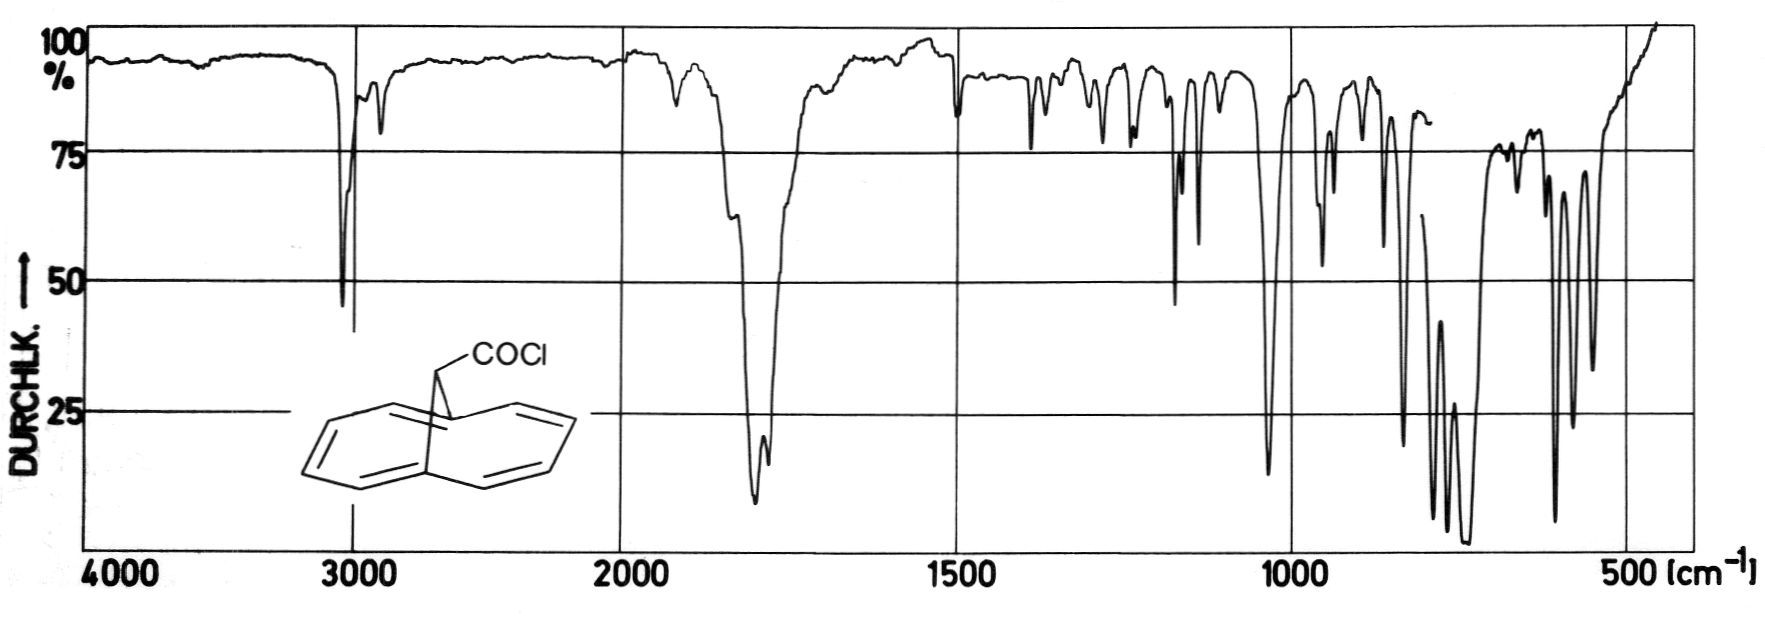
\includegraphics[width=14.94cm]{IR_033}
\begin{alltt}

3050 cm\raise0.5ex\hbox{-1}   =C-H    Valenzschwingung
2920 cm\raise0.5ex\hbox{-1}1  -C-H    Valenzschwingung (Brücke)
1810 cm\raise0.5ex\hbox{-1}   -C=O    Valenzschwingung
1790 cm\raise0.5ex\hbox{-1}
 750 cm\raise0.5ex\hbox{-1}   =C-H    Out-of-Plane-Schwingung

\(\overline{\hspace{7cm}}\)
\leavevmode\raise0.5ex\hbox{*}) destilliert 1. mit Chinolin, 2. mit Leinöl; Kp = 77\degree{}C

\newpage
\makebox[0.8\textwidth][c]{- 82 -}


UV-Spektrum (in Dioxan)

\(\lambda\)\lower0.5ex\hbox{max} = 256 (\(\epsilon\) = 52000), 295 (5700), 374 (270, Sch.), 383 (350),
392 (390) und 402 nm (290)

\leavevmode\raise0.5ex\hbox{1}H-NMR-Spektrum (in CCl\lower0.5ex\hbox{4}/TMS) s. Abb. 2 auf S. 10
  \(\tau\) [ppml
2.25 - 3.35 2 überlagerte AA'BB'-5ysteme   8 Annulenprotonen
9.33        Singulett                      1 Brückenproton

4.7 1,6-Methano-[10]annulen-11-carbonsäureazid (29)

Aktives Natriumazid \raise0.5ex\hbox{[121]}
In einem Mörser werden 20.0 g (0.3 Mol) Natriumazid und 1 ml
Hydrazinhydrat innig miteinander verrieben und 12 h stehen gelas-
sen. Man löst in 40 ml warmen Wasser und gibt die filtrierte
Lösung unter Rühren in 0.5 - 1 l dest. Aceton. Man saugt ab,
wäscht mit dest. Aceton und ebs. Äther und trocknet 15 min im
Hochvakuum. Es resultieren 15.0 - 17.0 g (75 - 85 \% d.Th.) eines
feinen weißen Pulvers.

Eine Lösung von 4.1 g (0.02 Mol) Carbonsäurechlorid (2B) in 40 ml
abs. Aceton wird auf 0\degree{}C gekühlt (Methanol/Trockeneis), wonach man
2.0 g (0.03 Mol) aktives Natriumazid in 8 ml Wasser so zutropft,
daß die Temperatur unter 0\degree{}C bleibt. Man rührt 15 min Bei 0\degree{}C
nach, gießt in 25 ml Eiswasser und extrahiert mit 2 x 50 ml Methy-
lenchlorid. Nach Trocknen über Magnesiumsulfat wird das Lösungs-
mittel abgezogen und der hellgelbe Rückstand (4.2 g) an Säule 1
mit Methylenchlorid chromatographiert. Nach dem Abziehen des Eluens
erhält man 4.0 g (0.019 Mol = 95 \% d.Th.) hellgelbe Nadeln mit dem
Zersetzungspunkt 111 - 115\degree{}C.
0.3 g Säureazid (29) werden in 2 ml Methylenchlorid gelöst und mit
2 ml Pentan versetzt. Bei -20\degree{}C erhält man 0.22 g (73 \% Ausbeute)
gelbe Quader vom Zersetzungsounkt 112 - 115\degree{}C.

\newpage
\makebox[0.8\textwidth][c]{- 83 -}


Elementaranalyse
C12H9N3O     ber.   C  68.24   H  4.30   N  19.89
211.225      gef.      67,92      4,23      


IR-Spektrum (4000-820 cm\raise0.5ex\hbox{-1} in CCl\lower0.5ex\hbox{4}, 820-500 cm\raise0.5ex\hbox{-1} in CS\lower0.5ex\hbox{2})
\end{alltt}
\hspace*{-0.5cm}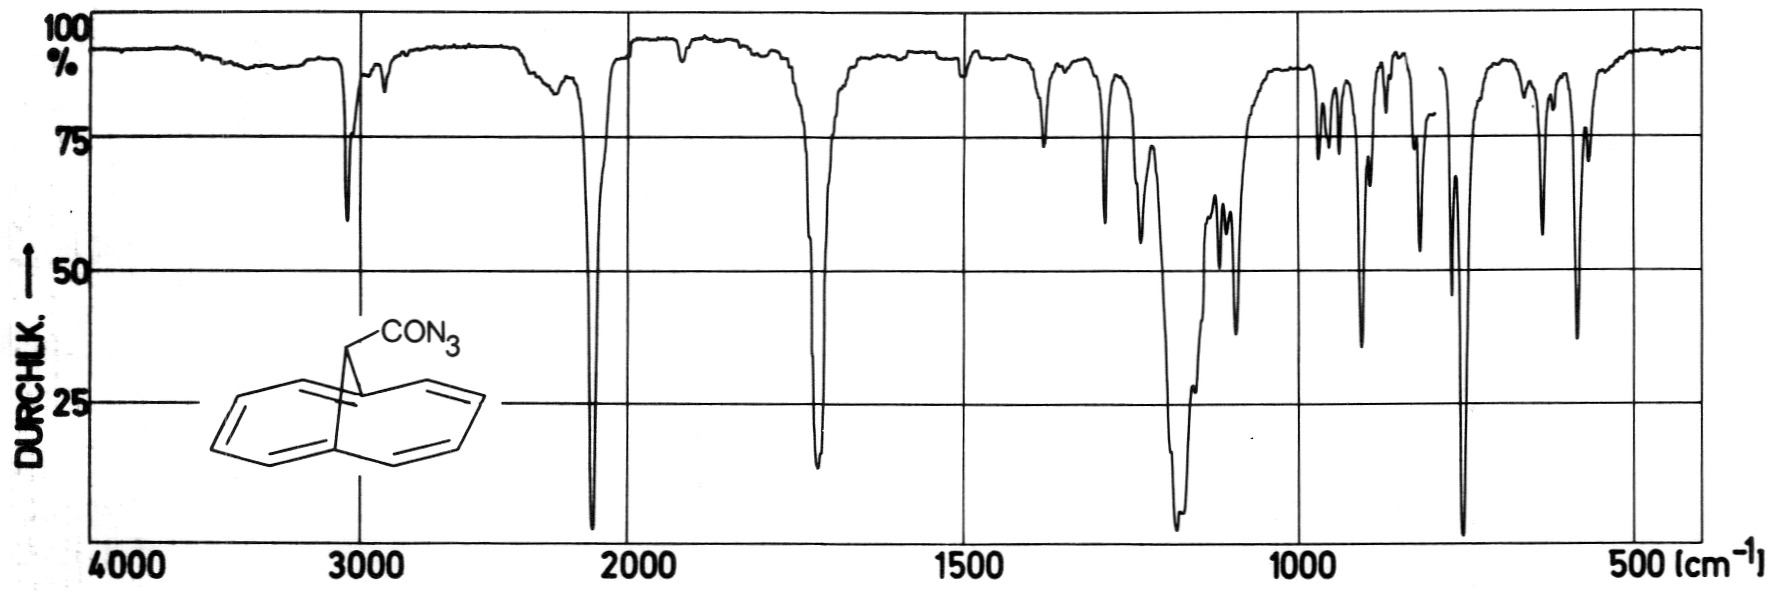
\includegraphics[width=14.94cm]{IR_034}
\begin{alltt}

3060 cm\raise0.5ex\hbox{-1}   =C-H    Valenzschwingung
2920 cm\raise0.5ex\hbox{-1}   -C-H    Valenzschwingung
2150 cm\raise0.5ex\hbox{-1}   -N3     Asymmetrische Streckschwingung
1725 cm\raise0.5ex\hbox{-1}   -C=O    Valenzschwingung
 764 cm\raise0.5ex\hbox{-1}   =C-H    Out-of-Plane-Schwingung

UV-Spektrum (in Dioxan)

\(\lambda\)\lower0.5ex\hbox{max} = 256 (\(\epsilon\) = 54800), 297 (6100), 374 (270, Sch.), 384 (330),
             393 (370) und 403 nm (270)

\leavevmode\raise0.5ex\hbox{1}H-NMR-Spektrum (in CD\lower0.5ex\hbox{2}Cl\lower0.5ex\hbox{2}/TM5) s. Abb. 3 auf S. 11
  \(\tau\) [ppm]

2.25 - 3.32  2 überlagerte AA‘BB‘-Systeme   8 Annulenprotonen
9.57         Singulett                      1 Brückenproton

\newpage
\makebox[0.8\textwidth][c]{- 84 -}


4.8 4-Nitrophenyl-N-[1,6-methano-[10]annulen-11-yl]carbaminat (31a)

Man erhitzt 3.2 g (0.015 Mal) Carbonsäureazid (29) mit 4.2 g (0.03
Mol) 4-Nitrophenol in 20 ml Benzol auf 70 - 80\degree{}C, wobei sich die
zunächst klare gelbe Lösung unter Gasentwicklung braun Färbt. Nach
15 min erhöht man die Temperatur auf 80 - 90\degree{}C. Nach 2.5 h lässt man
abkühlen, gibt die Lösung, aus der unter Umständen schon 4-Nitro-
phenol auskristallisiert, auf Säule 2 und eluiert mit Methylen-
chlorid. Der Rückstand nach Abziehen des Lösungsmittels (3.6 g)
wird in wenig Methylenchlorid aufgenommen und erneut chromatogra-
phiert (Säule 4; Eluens: Methylenchlorid). Nach Abziehen des Lösungs-
mittels hinterbleiben 3.4 g (0.011 Mol = 70 \% d.Th.) hellgelbes
Kristallpulver vom Fp = 143 - 145\degree{}C, das für weitere Reaktionen
so eingesetzt werden kann.
0.3 g Carbaminat (31a) werden in 1.5 ml Chloroform gelöst und mit
1 ml Pentan versetzt. Bei -20\degree{}C kristallisieren 0.2 g (67 \% Aus-
beute) feine hellgelbe Nadeln vom Fp = 144 - 145\degree{}C aus.

Elementaranalyse
C18H14N204     ber.    C  67.08   H  4.38   N  8.69
 322.323       gef.       66.98      4.29      8.58

IR-Spektrum (in Kaliumbromid)
\end{alltt}
\hspace*{-0.4cm}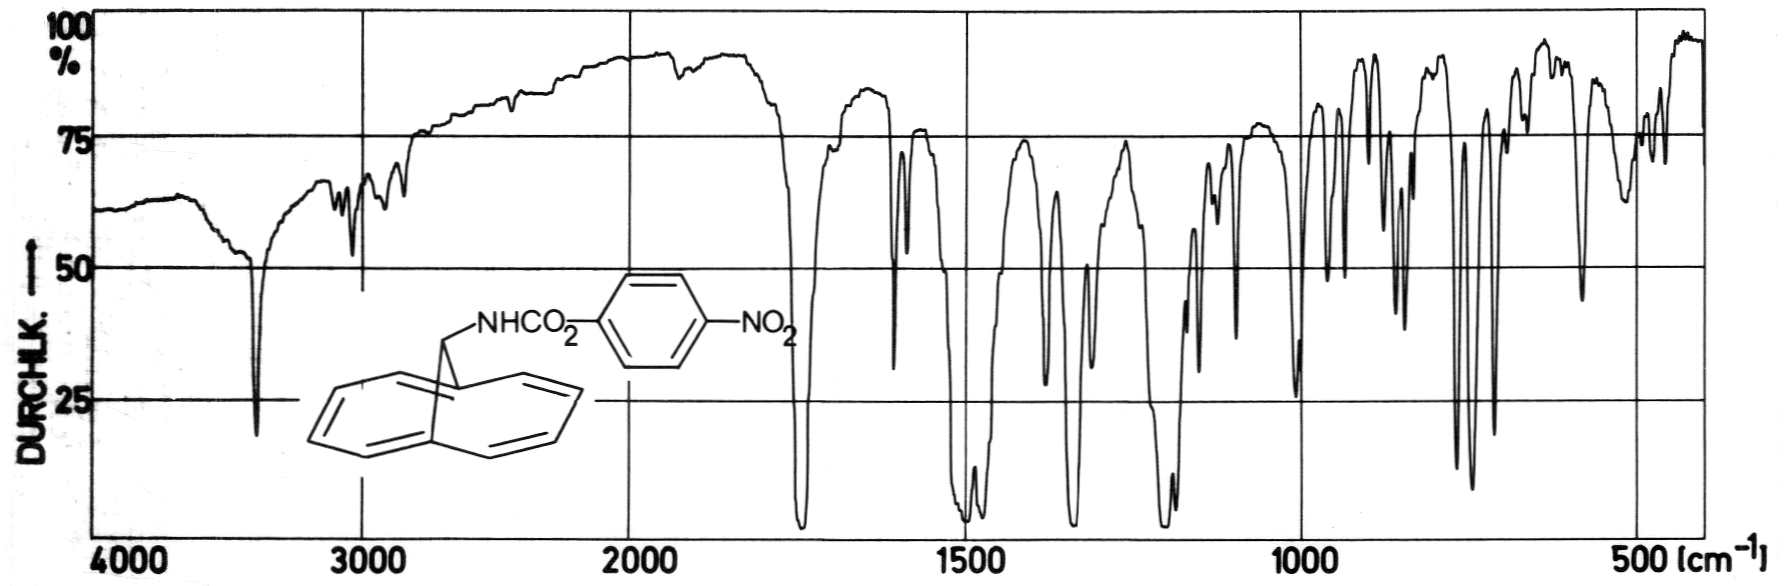
\includegraphics[width=15.12cm]{IR_035}
\begin{alltt}

3410 cm\raise0.5ex\hbox{-1}    -N-H     Valenzschwingung
3115 cm\raise0.5ex\hbox{-1}
3090 cm\raise0.5ex\hbox{-1}

\newpage
\makebox[0.8\textwidth][c]{- 85 -}


3055 cm\raise0.5ex\hbox{-1}    =C-H     Valenzschwingung
2935 cm\raise0.5ex\hbox{-1}    -C-H     Valenzschwingung
1752 cm\raise0.5ex\hbox{-1}    -C=O     Valenzschwingung
1214 cm\raise0.5ex\hbox{-1}    -C-O     Valenzschwingung
 780 cm\raise0.5ex\hbox{-1}    =C-H     Out-of-Plane-Schwingung

UV-Spektrum (in Dioxan)

\(\lambda\)\lower0.5ex\hbox{max} = 256 (\(\epsilon\) = 58700), 295 (13400, Sch.), 887 (282, Sch.)
             und 397 nm (188, Sch.)

\leavevmode\raise0.5ex\hbox{1}H-NMR-Spektrum (in CDCl\lower0.5ex\hbox{3}/TMS) s. Abb. 4 auf S. 14
  \(\tau\) [ppm]
1.85 - 3.18   AB-System der 4 Benzolprotonen    12 aromatische Protonen
               \(\nu\)\lower0.5ex\hbox{A} = 1.94 \(\tau\)
               \(\nu\)\lower0.5ex\hbox{B} = 2.94 \(\tau\)
               J\lower0.5ex\hbox{AB} 5 Hz

2.42 - 3.18   2 AA'BB'-Systeme der 8 Annulen-
              protonen, überlagert vom B-Teil
              der Benzolprotonen
6.16          Dublett (J = 13 Hz)                1 Amidproton
8.43          Dublett (J = 1a Hz)                1 Brückenproton


4.9 1,6-Methano-[10]annulen-11-isocyanat (30)

Man löst 0.644 g (0.002 M01) 4-Nitrophenylcarbaminat (31a) in 10 ml
Methylenchlorid und gibt bei 0\degree{}C zunächst 0.245 g (0.0024 Mol) Tri-
äthylamin zu. Danach werden 0.26 g (0.0024 M01) Trimethylchlorsilan
in 4 ml Methylenchlorid tropfenweise zugefügt. Man rührt 5 h bei
Raumtemperatur und zieht das Lösungsmittel bis auf einen kleinen
Rest am Rotationsverdampfer ab. Der Rückstand wird mit Methylen-
chlorid an Säule 2 chromatographiert, wobei man die bei 350 nm

\newpage
\makebox[0.8\textwidth][c]{- 86 -}


hellblau fluoreszierende Substanz auffängt. Nach Abziehen des
Methylenchlorids verbleiben 0.26 g (0.0014 Mal = 71 \% d.Th.) hell-
gelbe Kristalle vom Fp = 63 - 64\degree{}C. Umkristallisieren aus 4 ml
Äther und 2 ml Pentan ergibt 0.18 g (0.001 Mol = 50 \% d.Th.) gelbe
Kristallplatten vom Fp = 64 - 65\degree{}C.

Elementaranalyse
C12H9NO    ber.     C  78.67   H  4.95   N  7.65
183.212    gef.        78.50      5.11      7.70

IR-Spektrum s. Abb. 5 auf S. 15

3042 cm\raise0.5ex\hbox{-1}    =C-H     Valenzschwingung
2950 cm\raise0.5ex\hbox{-1}    -C-H     Valenzschwingung
2258 cm\raise0.5ex\hbox{-1}    -N=C=O   Asymmetrische Streckschwingung
 766 cm\raise0.5ex\hbox{-1}    =C-H     Out-of-Plane-Schwingung
 594 cm\raise0.5ex\hbox{-1}    -N=C=O   Bending-Schwingung

UV-Spektrum (in Dioxan)

\(\lambda\)\lower0.5ex\hbox{max} = 255 (s = 61800), 297 (5750), 381 (300), 390 (320)
und 400 nm (225, Sch.)

 

\leavevmode\raise0.5ex\hbox{1}H-NMR-Spektrum (in CCl\lower0.5ex\hbox{4}/TMS) s. Abb. 6 auf S. 16
  \(\tau\) [ppm]
2.45 - 3.22   2 enge AA'BB'-Systeme  8 Annulenprotonen
8.79          Singulett              1 Brückenproton

\newpage
\makebox[0.8\textwidth][c]{- 87 -}


4.10 11-Acetoxy-1,6-methano-[10]annulen (35) \raise0.5ex\hbox{[42]}
 
Man erhitzt 11.0 g (0.05 Mol) 11-Brom-1,6-methano-[10]annulen (25)
und 12.5 g (0.075 Mol) Silber(I)acetat in 600 ml Eisessig 24 h
unter Rückfluss. Nach dem Abkühlen filtriert man von den ausgeschie-
denen Silbersalzen ab und gibt auf 1.2 l Wasser. Der Filterinhalt
wird sorgfältig mit 600 ml Pentan gewaschen, das dann zum Ausschüt-
teln der wässrigen Phase dient. Nach Abtrennen der organischen
Phase wird mit weiteren 4 x 400 ml Pentan ausgeschüttelt und mit
5 \%iger Natriumhydrogencarbonat-Lösung neutral gewaschen. Nach
Trocknen über Magnesiumsulfat und Abziehen des Lösungsmittels hin-
terbleiben 7.8 - 9.0 g gelber Rückstand, der aus 150 - 180 ml
Petroläther (40-70) umkristallisiert wird. Man erhält 7.1 - 7.8 g
(0.036 - 0.039 Mol = 71 - 78 \% d.Th.) gelbe Kristallnadeln vom
Fp = 92 - 93\degree{}C.


4.11 11-Hydroxy-1,5-methano-[10]annulen (20) \raise0.5ex\hbox{[42,59]}

Unter Argon tropft man zu 4.4 g (0.18 Mol) Magnesiumspänen eine
Lösung von 25.5 g (0.18 Mol) Methyljodid\leavevmode\raise0.5ex\hbox{*}) in 300 ml Äther. Zu-
nächst lässt man schnell zutropfen, wenn dann jedoch die Reaktion
angesprungen ist, tropft man so zu, daß die Mischung eben am Rück-
flußkühler siedet. Nach beendeter Zugabe wird 5 min nachgerührt
und auf 0\degree{}C abgekühlt. Innerhalb von 10 min werden 6.0 g (0.03 Mol)
Acetat (35) in fester Form zugegeben. Man rührt 1 h bei 0\degree{}C -
dabei fallen Magnesiumsalze aus - und eine weitere Stunde bei Raum-
temperatur. Es wird in Eiswasser gekühlt und tropfenweise mit
gesättigter Ammoniumchlorid-Lösung versetzt. Nach Zersetzung der
überschüssigen GRIGNARD-Verbindung kann der Rest der Ammoniumchlo-
ridlösung (insgesamt 180 ml) schnell zugegeben werden. Man gießt in
200 ml Äther, trennt die Phasen und wäscht die ätherische Phase mit
100 ml gesättigter Ammoniumchlorid-Lösung und 100 ml Wasser. Nach

\(\overline{\hspace{7cm}}\)
\leavevmode\raise0.5ex\hbox{*}) Uber Quecksilber mit Kolonne destilliert; Kp = 42.5\degree{}C

\newpage
\makebox[0.8\textwidth][c]{- 88 -}


Trocknen über Natriumsulfat wird das Lösungsmittel im Vakuum ent-
fernt und der verbleibende hellgelbe Rückstand (4.8 g) in 30 ml
Äther gelöst und mit 30 ml Pentan versetzt. Nach Zugabe eines
Impfkristalls kristallisieren bei -20\degree{}C 3.4 g (0.022 Mol = 72 \% d.
Th.) monokline Prismen vom Fp = 70 - 71\degree{}C.


4.12 Oxidation des 11-Hydroxy-1,6-methano-[10]annulens (20) \leavevmode\raise0.5ex\hbox{*})

mit Chrom(VI)oxid/Pyridin in Methylenchlorid \raise0.5ex\hbox{[66]}
Unter Eiskühlung werden zu 0.95 g (0.012 Mol) Pyridin in 15 ml
abs. Methylenchlorid 0.6 g (0.006 Mol) gepulvertes Chrom(VI)oxid
gegeben. Nach 15 min Nachrühren gibt man zu der burgunderroten
Lösung 0.158 g (0.001 Mol) Alkohol (20) in 1 ml Methylenchlorid,
wobei sofort ein schwarzer Niederschlag ausfällt, von dem nach
15 min Rühren abdekantiert wird. Das Lösungsmittel wird im Vakuum
abgezogen, der Rückstand mit 20 ml Äther aufgenommen und mit
5 \%iger Natronlauge, 5\%iger Salzsäure und Wasser (jeweils 10 ml)
gewaschen. Nach Trocknen über Magnesiumsulfat wird der Äther ab-
gezogen. Der Rückstand (0.08 g = 63 \% d.Th.] besteht laut Gas-
chromatogramm (Säule A) zu über 95 \% aus Naphthalin.

mit Blei(IV)acetat in Pyridin \raise0.5ex\hbox{[65]}
Unter Eiskühlung gibt man zu 5 ml Pyridin und 0.158 g (0.001 Mol)
Alkohol (20) 0.443 g (0.001 Mol) Blei(IV)acetat. Nach 1 h Rühren
gießt man die braune Lösung in 20 ml Wasser und extrahiert mit 2 x
10 ml Äther. Nach Waschen mit jeweils 10 ml 5\%iger Salzsäure und
Wasser trocknet man über Magnesiumsulfat und zieht das Lösungsmit-
tel ab. Der Rückstand (0.11 g = 85 \% d.Th.J besteht laut Gaschroma-
togramm (Säule A) zu über 95 \% aus Naphthalin.

 
\(\overline{\hspace{7cm}}\)
\leavevmode\raise0.5ex\hbox{*}) Versuche mit ähnlichen Oxidationsmitteln wurden bereits von
   H. Lepper \raise0.5ex\hbox{[42]} beschrieben.

\newpage
\makebox[0.8\textwidth][c]{- 89 -}


mit aktivem Mangan(IV)oxid in Aceton \raise0.5ex\hbox{[63]}
Zu einer Lösung von 0.158 g (0.001 Mol) Alkohol (20) in 12 ml abs.
Aceton gibt man unter Eiskühlung 1.7 g (0.02 Mol) aktives Mangan-
(IV)oxid. Man lässt 1 d bei Raumtemperatur rühren, filtriert und
engt das Filtrat ein. Der Rückstand (0.09 g = 70 \% d.Th.) besteht
laut Gaschromatogramm (Säule A) zu über 90 \% aus Naphthalin.

 

4.13 11-Oxo-1,6-methano-[10]annulen (15)

Oxidation mit Dimethylsulfoxid und Acetanhydrid
Zu einer Lösung von 0.158 g (0.001 Mal) Alkohol (20) in 3 ml
DMSO \leavevmode\raise0.5ex\hbox{*}) gibt man 2 ml Acetanhydrid und lässt vier Tage bei Raum-
temperatur rühren. Man gießt in 20 ml Wasser, extrahiert mit 2 x
10 ml Äther, wäscht mit 2 x 5 ml gesättigter Natriumhydrogencarbo-
natlösung und 10 ml Wasser. Nach Trocknen über Magnesiumsulfat und
Abziehen des Äthers hinterbleiben 0.8 g gelbes Öl, aus dem beim
Stehenlassen gelbe Kristalle ausfallen. Man chromatographiert an
Säule 4 mit Chloroform, wobei zwei Fraktionen eluiert werden:

1) Thiomethoxymethyl-[1,6-methano-[10]annulen-11-yl]äther (39):
Man isoliert 0.1 g (0.0005 Mol = 46 \% d.Th.) hellgelbe Kri-
stalle, die beim Umkristallisieren aus 3 ml n-Hexan 0.05 g
(0.0002 Mol = 28 \% d.Th.) hellgelbe Nadeln vom Fp = 81 - 83\degree{}C
ergeben. Abermaliges Umkristallisieren führt zur Schmelz-
punktskonstanz bei 83 - 85\degree{}C.

Elementaranalyse
C13H14OS    ber.   C   71.52   H    6.46    S 14.69
218.32      gef.       71.86        6.40      14.36

 
\(\overline{\hspace{7cm}}\)
\leavevmode\raise0.5ex\hbox{*}) Zur Reinigung des käuflichen DMSO gibt man etwa 1 l auf einen
   mit Aluminiumoxid Woelm basisch Akt. II gefüllten 500 ml Tropf-
   trichter (25 cm lang; \(\Phi\)\lower0.5ex\hbox{i} = 7.5 cm) und lässt die Flüssigkeit
   langsam durchsickern, wobei sich die Säulenfüllung zunächst
   stark erwärmt. Wenn sich die Säule abgekühlt hat, besitzt das
   auslaufende DMSO die benötigte Qualität.

\newpage
\makebox[0.8\textwidth][c]{- 90 -}


IR-Spektrum (in Kaliumbromid)
\end{alltt}
\hspace*{-0.4cm}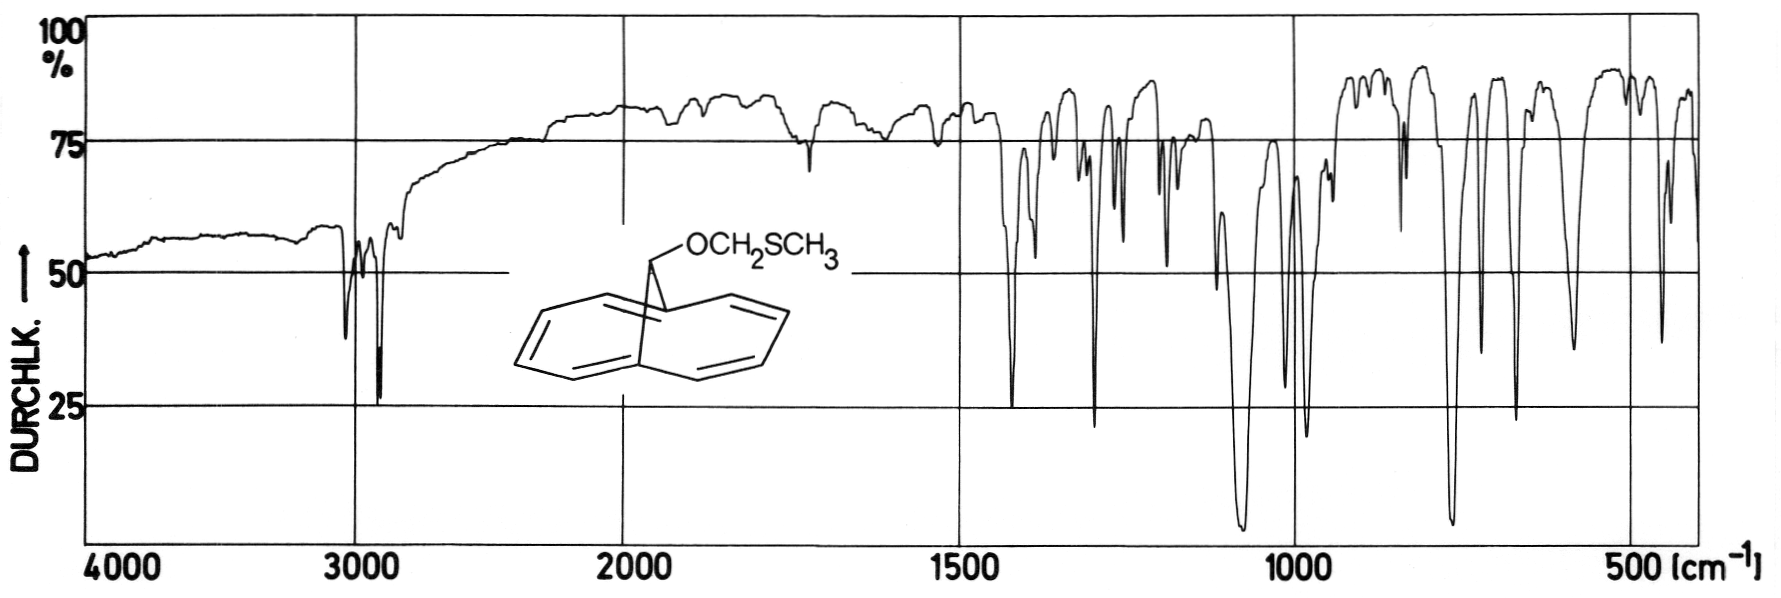
\includegraphics[width=15.08cm]{IR_036}
\begin{alltt}

3045 cm\raise0.5ex\hbox{-1}    =C-H     Valenzschwingung
2080 cm\raise0.5ex\hbox{-1}    -C-H     Valenzschwingung
2030 cm\raise0.5ex\hbox{-1}    O-C-H    Valenzschwingung
2020 cm\raise0.5ex\hbox{-1}
1429 cm\raise0.5ex\hbox{-1}    -CH2-    Deformationsschwingung
1392 cm\raise0.5ex\hbox{-1}    -CH3     Deformationsschwingung
1084 cm\raise0.5ex\hbox{-1}    -C-O     Valenzschwingung
 778 cm\raise0.5ex\hbox{-1}    =C-H     Out-of-Plane-Schwingung


UV-Spektrum (in Cyclohexan)

\(\lambda\)\lower0.5ex\hbox{max} = 256 (\(\epsilon\) = 54800), 294 (5800), 380 (220), 389 (240)
und 399 nm (175)

\leavevmode\raise0.5ex\hbox{1}H-NMR-Spektrum (in CCl\lower0.5ex\hbox{4}/TMS) s. Abb. 9 auf S. 24
  \(\tau\) [ppm]
2.43 - 3.25      2 AA'BB'-Systeme     8 Annulanpratonen
6.20             Singulett            2 Methylenprotonen
8.27             Singulett            3 Methylprotonen
8.50             Singulett            1 Brückenproton

\newpage
\makebox[0.8\textwidth][c]{- 91 -}


2) 11-Oxo-1,6-methano-[10]annulen (15)
   Es werden 0.7 g gelbes Öl, aus dem sich Kristalle abscheiden,
   erhalten. Man digeriert mit 3 x 3 ml eiskaltem Pentan, wobei
   0.055 g (0.0004 Mol = 35 \% d.Th.) 11-Oxo_1‚6-methano-[10]an-
   nulen (15) als gelbgrüne Kristallblättchen vom Fp = 185 - 186\degree{}C
   resultieren.


Oxidation mit Dimethylsulfoxid und Dicyclohexylcarbodiimid

Pyridintrifluoracetet (PTFA)
Zu einer Lösung von 11.4 g (0.1 Mol) Trifluoressigsäure in 100 ml
abs. Äther tropft man unter Eiskühlung und Rühren eine Lösung von
7.9 g (0.1 Mol) abs. Pyridin in 100 ml Äther. Nach Verdünnen mit
200 ml abs. Pentan wird abgenutscht, mit Pentan gewaschen und im
Hochvakuum getrocknet. Man erhält 18.0 g (93 \% d.Th.) eines weißen
hygroskopischen Kristallpulvers.

Zu einer Mischung von 2.0 g (0.01 Mol) PTFA, 12.4 g (0.05 M01) DCC,
50 ml DMSO und 50 ml abs. Benzol gibt man 3.2 g (0.02 Mol) Alkohol
(20) in fester Form. Man fügt jeweils nach 5 h, 20 h, 30 h und
40 h Reaktionszeit 0.1 g (0.0005 Mol) PTFA zu. Dünnschichtchroma-
tographisch können nach 48 h nur noch geringe Mengen Edukt (20)
nachgewiesen werden. Man verdünnt die nun gelbbraune, intensiv nach
Dimethylsulfid riechende Reaktionsmischung, aus der sich Dicyclo-
hexylharnstoff abgeschieden hat, mit 150 ml Äther, filtriert, wäscht
das Filter mit 2 x 50 ml Äther und verdünnt mit weiteren 200 ml
Äther, worauf mit 3 x 100 ml Wasser gewaschen wird. Nach Trocknen
über Magnesiumsulfat und Abziehen des Äthers im Vakuum hinterblei-
ben etwa 10 g öliger, halbkristalliner Rückstand, der mit 100 ml
eiskaltem Pentan digeriert wird. Man saugt ab und kocht den festen
Filterinhalt (2.7 g) mit 250 ml warmen Äther und filtriert vom Un-
gelösten. Bei -20\degree{}C kristallisieren 2.0 g (0.013 Mol = 54 \% d.Th.)
hellgelb-grüne Nadeln vom Fp = 185 - 186\degree{}C aus.

\newpage
\makebox[0.8\textwidth][c]{- 92 -}


Oxidation mit Dimethylsulfoxid und Äthyl-[3-(dimethylamino)propyl]-
carbodiimid-hydrochlorid

Unter Rühren gibt man 25 ml Benzol, 1.0 g (0.005 Mol) PTFA, 5.7 g
(0.08 Mol) Äthyl-[3-(dimetnylamino)propyl]carbodiimid-hydrochlo-
rid \raise0.5ex\hbox{[75]} und 2e ml DMSO zusammen und fügt 1.6 g (0.01 Mol) Alkohol
(20) in fester Form zu. Innerhalb von 10 min klärt sich die schau-
mige Suspension unter leichter Wärmeentwicklung zu einer hellgelben
Lösung. Jeweils nach 5 h, 20 h, 30 h und 40 h versetzt man mit
0.05 g (0.00025 Mal) PTFA. Nach 40 h Rühren verdünnt man mit 100 ml
Äther und gießt auf 100 ml Wasser. Man trennt die Phasen und extra-
hiert das Wasser nochmals mit 50 ml Äther. Die Ätherphase wird mit
4 x 50 ml Wasser gewaschen und über Magnesiumsulfat getrocknet.
Abziehen des Lösungsmittels im Vakuum ergibt 1.6 g gelben, festen
Rückstand, der in 100 ml Äther gelöst wird. Beim Abkühlen auf
-20\degree{}C resultieren 1.2 g (0.008 Mol = 77 \% d.Th.) hellgelb-grüne
Kristallnadeln vom Fp = 186 - 188\degree{}C. '
Umkristallisieren von 0.3 g Keton (15) aus 7 ml Methanol führt zu
0.22 g (73 \% Ausbeute) hellgelb-grüner Kristallblättchen vom Fp =
188 - 189\degree{}C.

Elementaranalyse
C11H8O        ber. C  84.59   H  5.16
156.186               84.36      5.44

IR-Spektrum (in Caesiumjodid)
\end{alltt}
\hspace*{-0.4cm}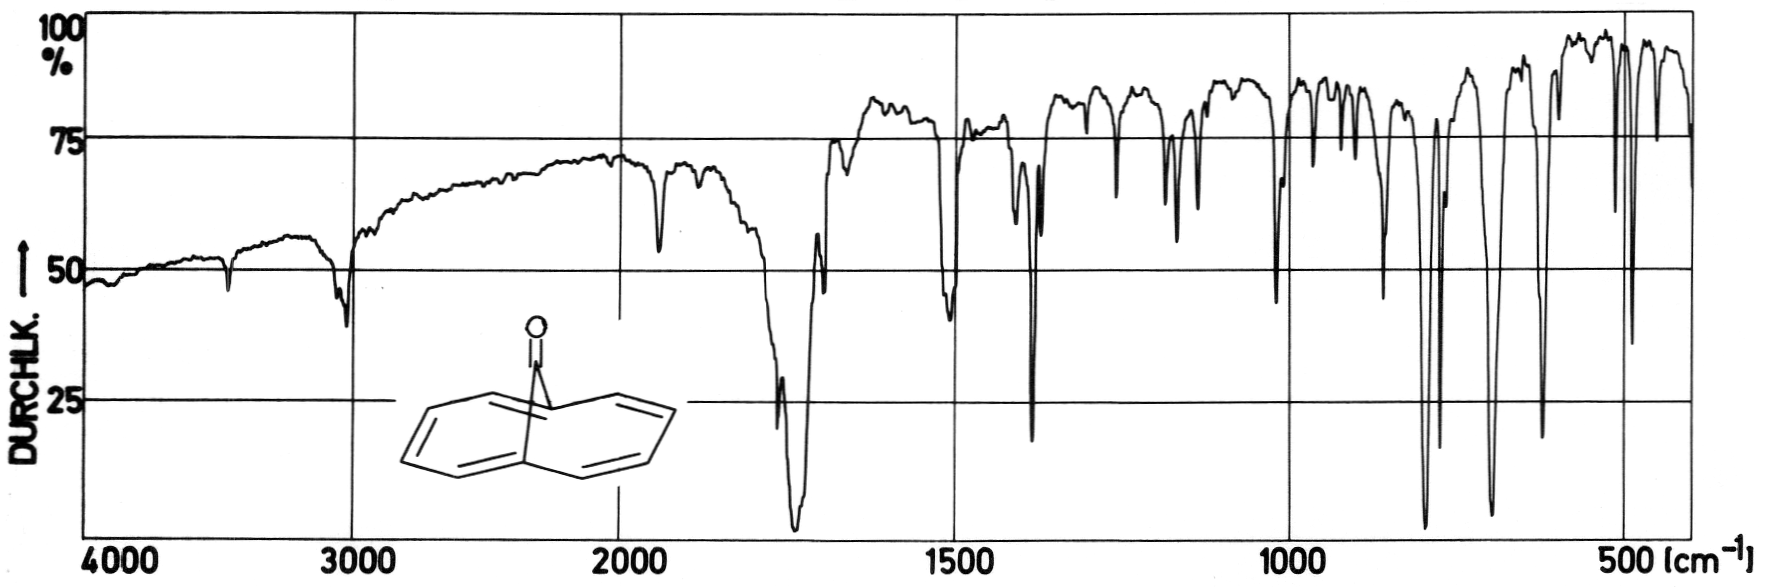
\includegraphics[width=15.15cm]{IR_037}
\begin{alltt}

\newpage
\makebox[0.8\textwidth][c]{- 93 -}


3065 cm\raise0.5ex\hbox{-1}    =C-H     Valenzschwingung
3030 cm\raise0.5ex\hbox{-1}
1740 cm\raise0.5ex\hbox{-1}    -C=O     Valenzschwingung
1510 cm\raise0.5ex\hbox{-1}    -C=C-
 780 cm\raise0.5ex\hbox{-1}    =C-H     Out-of-Plane-Schwingung

UV-Spektrum (in Cyclohexan)

\(\lambda\)\lower0.5ex\hbox{max} = 252 (\(\epsilon\) = 74000), 296 (6700), 352 (75), 364 (105), 372 (149),
       381 (198), 389 (206), 295 (157, Sch.) und 403 nm (216)


\leavevmode\raise0.5ex\hbox{1}H-NMR-Spektrum (in CDCl\lower0.5ex\hbox{3}/TMS, 60 MHz) s. Abb. 11 auf S. 28
  \(\tau\) [ppm]
2.27 - 2.90    AA'BB'-System     8 Annulenprotonen


\leavevmode\raise0.5ex\hbox{1}H-NMR-Spektrum (in CD\lower0.5ex\hbox{2}Cl\lower0.5ex\hbox{2}, TMS als Lock, 100 MHz)

Die exakten Parameter der Protonenanalyee des 11-Oxo-1‚6-methano-
[10]annulens (35) sind in Tabelle 2 auf S. 33 aufgeführt.

\leavevmode\raise0.5ex\hbox{13}C-NMR-Spektrum (in CCl\lower0.5ex\hbox{4}/CDCl\lower0.5ex\hbox{3}/TMS) s. Abb. 12 auf S. 29
\end{alltt}
\hspace{3.5cm}
% 11-Oxo- 1,6-methano-[10]annulen (15) mit Atomnummern
\chemfig[atom style={scale=\normalscale}]{%
=_[:60,,,,shrtdbl={0pt}{3.5pt}]@{n9}%
-[:12]@{n10}%
=_[:-12]@{n1}%
(-[:-252]?@{n11}(=[:90,0.6]O))% 1,6 Brücke
-[:12]@{n2}%
=_[:-12,,,,shrtdbl={4pt}{0pt}]@{n3}%
-[:-120]@{n4}%
=_[:-168]@{n5}%
-[:168]?@{n6}%
=_[:-168,,,,shrtdbl={1pt}{1pt}]@{n7}%
-[:168]@{n8}%
}%
\chemmove{
    \node at (n1) [above right=-0.05 and -0.1] {\scriptsize\textsf{1}};
    \node at (n2) [above right=-0.05 and -0.1] {\scriptsize\textsf{2}};
    \node at (n3) [right=-0.05] {\scriptsize\textsf{3}};
    \node at (n4) [right=0.03] {\scriptsize\textsf{4}};
    \node at (n5) [below=-0.05] {\scriptsize\textsf{5}};
    \node at (n6) [below=-0.05] {\scriptsize\textsf{6}};
    \node at (n7) [below=-0.05] {\scriptsize\textsf{7}};
    \node at (n8) [left=-0.05] {\scriptsize\textsf{8}};
    \node at (n9) [left=0] {\scriptsize\textsf{9}};
    \node at (n10) [above=-0.05] {\scriptsize\textsf{10}};
    \node at (n11) [right] {\scriptsize\textsf{11}};
}%
\begin{alltt}
          \(\delta\) = 129.4           C-1, C-6
          \(\delta\) = 123.3           C-2, C-5, C-7, C-10
          \(\delta\) = 123.7           C-3, C-4, C-8, C-9
          \(\delta\) = 197.4           C-11

Massenspektrum (100 eV) s. Abb. 10 auf S. 27

m/e       156     (3 \%)       M+
          128   (100 \%)       M+ - CO
          127    (15 \%)       M+ - CO - H

\newpage
\makebox[0.8\textwidth][c]{- 94 -}


Alternativsynthese nach S. Ito \raise0.5ex\hbox{[112]}

11-Oxobicyclo[4.4.1]undecatrien-(2‚4,8) (59)

In einer 100 ml - Ampulle kondensiert man ca. 30 ml (~0.4 Mol)
Butadien-(1,3) bei -78\degree{}C und gibt 0.2 g 1,4-Hydrochinon, 5.3 g
(0.05 Mol) Tropon \raise0.5ex\hbox{[106]} und 30 ml Xylol zu, wonach man 12 h bei
130\degree{}C erhitzt. Nach dem Abkühlen spült man die gelbe homogene
Lösung mit Methylenchlorid in einen Kolben und zieht alle flüch-
tigen Bestandteile im Wasserstrahlvakuum ab. Der Rückstand wird
im Hochvakuum destilliert, wobei 7.0 g (0.044 Mol = 87 \% d.Th.)
Cycloadditionsprodukt (59) vom Kp = 58 - 62\degree{}C bei 0.15 mm Hg als
schwach grünliche Flüssigkeit übergehen. Für die nachfolgende
Dehydrierung ist diese Substanz rein genug. Eine weitergehende
Säuberung erfolgt durch Ketalisierung und anschließende Ketal-
spaltung.

11-Oxobicyclo[4.4.1]undecatrien-(2,4,8)-äthylenketal (60)
Man erhitzt 1.6 g (0.01 Mol) Keton (59) mit etwas p-Toluolsulfon-
säure, 2 ml Benzol und 0.75 g (0.012 Mol) Äthylenglykol 14 h am
Wasserabscheider. Nach dem Abkühlen nimmt man die rotbraune
Lösung mit 10 ml Äther auf, wäscht mit 10 ml Wasser, schüttelt
die wässrige Phase nochmals mit 10 ml Äther aus und wäscht dann
die ätherischen Phasen mit 10 ml 5 \%iger Natronlauge sowie 10 ml
Wasser. Nach dem Trocknen über Kaliumcarbonat und Abziehen des
Lösungsmittels hinterbleiben 2.1 g grünlicher kristalliner Bück-
stand, der im Hochvakuum bei 82 - 88\degree{}C und 0.1 mm Hg destilliert
wird. Das übergehende farblose Öl (1.6 g) wird in 2 ml Methanol
unter Erwärmen gelöst und mit 3 ml Hexan versetzt. Bei 5\degree{}C kri-
stallisieren allmählich 1.1 g (0.005 Mol = 54 \% d.Th.) farblose,
rhombische Platten vom Fp = 75 - 76\degree{}C. Zweimaliges Umkristalli-
sieren einer kleinen Probe aus Methanol/Hexan führt zur Schmelz-
punktskonstanz bei 77 - 78\degree{}C.

Elementaranalyse
C13H16O2     ber.    C  76.44   H  7.90
204.271      gef.       76.28      8.00

\newpage
\makebox[0.8\textwidth][c]{- 95 -}


IR-Spektrum (4000-820 cm\raise0.5ex\hbox{-1} in CCl\lower0.5ex\hbox{4}, 820-500 cm\raise0.5ex\hbox{-1} in CS\lower0.5ex\hbox{2})
\end{alltt}
\hspace*{-0.5cm}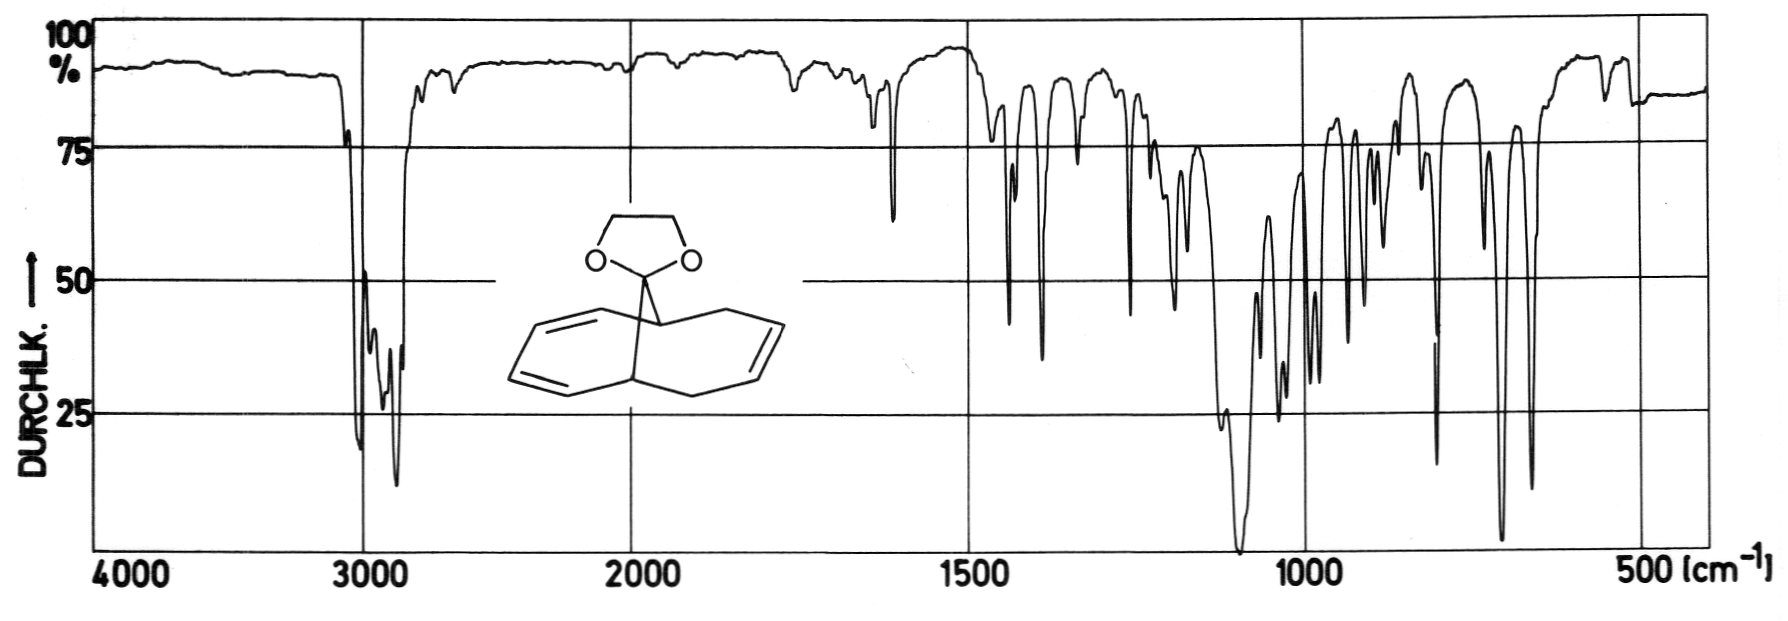
\includegraphics[width=15.14cm]{IR_038}
\begin{alltt}

3020 cm\raise0.5ex\hbox{-1}     =C-H     Valenzschwingung
2985 cm\raise0.5ex\hbox{-1}     -C-H     Valenzschwingung
2940 cm\raise0.5ex\hbox{-1}
2890 cm\raise0.5ex\hbox{-1}
1646 cm\raise0.5ex\hbox{-1}     -C=C-
1616 cm\raise0.5ex\hbox{-1}
1448 cm\raise0.5ex\hbox{-1}     -CH2-    Deformationsschwingung
1400 cm\raise0.5ex\hbox{-1}
1108 cm\raise0.5ex\hbox{-1}     -C-O     Valenzschwingung


\leavevmode\raise0.5ex\hbox{1}H-NMR-Spektrum (in CDCl\lower0.5ex\hbox{3}/TMS)
\end{alltt}
\hspace*{-0.25cm}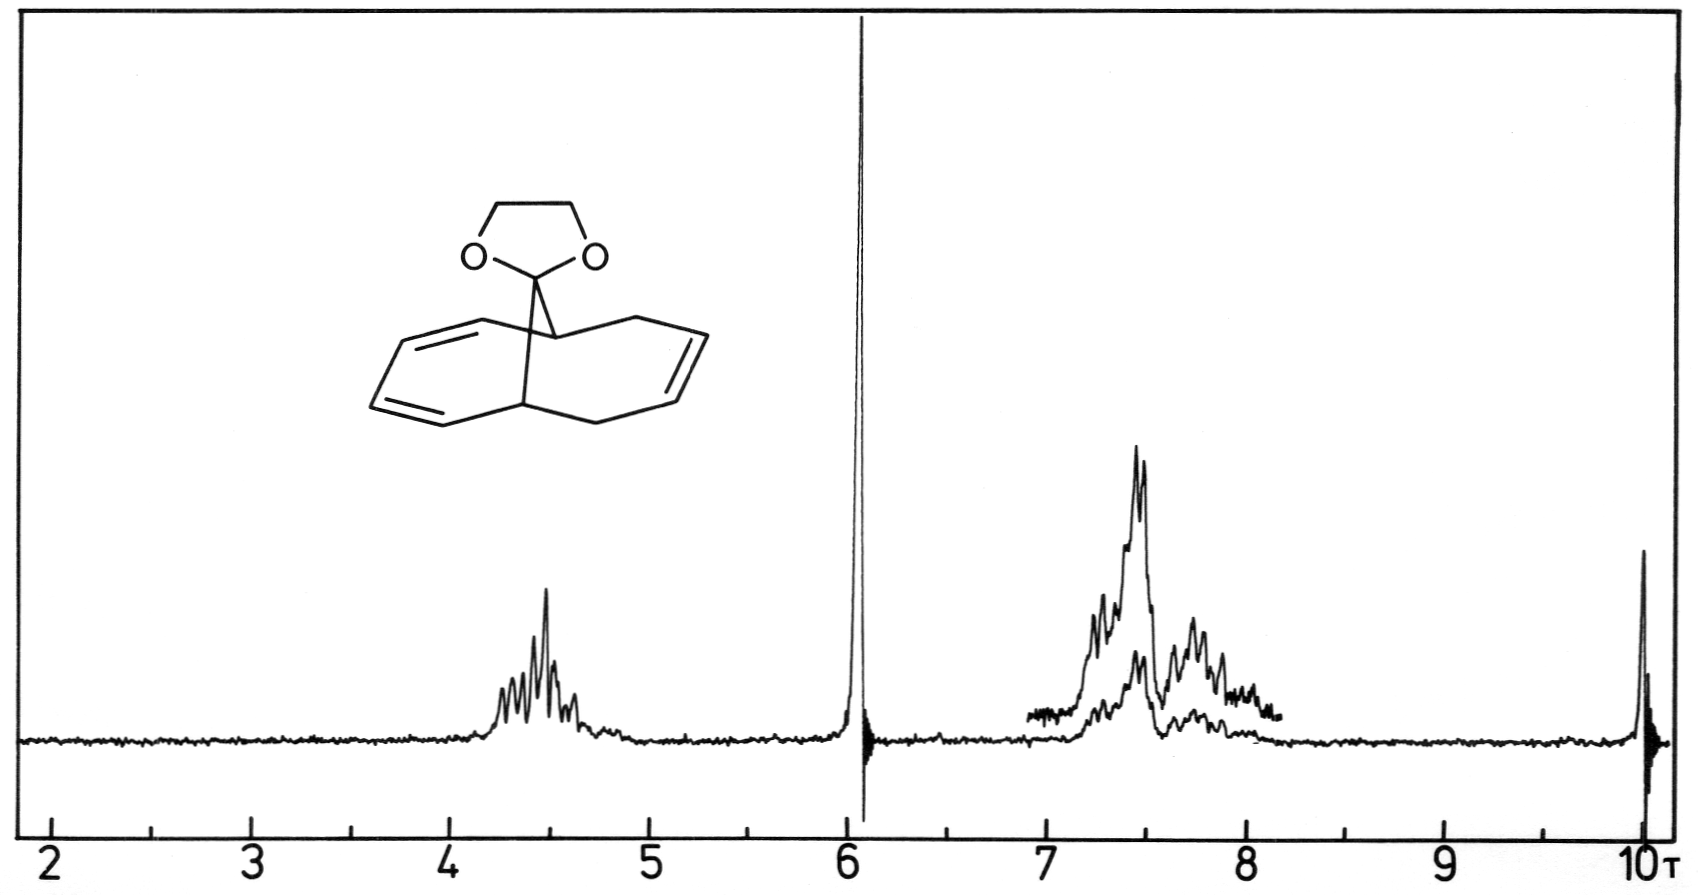
\includegraphics[width=14.38cm]{NMR_039}
\begin{alltt}
\newpage
\makebox[0.8\textwidth][c]{- 96 -}


  \(\tau\) [ppm]
4.13 - 4.92    Multiplett        6 olefinische Protonen
6.06           Singulett         4 Ketalprotonen
7.13 - 8.15    Multiplett        6 allylische Protonen

UV-Spektrum (in Cyclohexan)

\(\lambda\)\lower0.5ex\hbox{max} = 241 (\(\epsilon\) = 4300, Sch.), 247 (6400), 256 (7450)
             und 267 nm (4800)

11-Oxobicyclo[4.4.1]undecatrien-(2,4,5) (59) durch Spaltung
des 11-Oxobicyclo[4.4.1]undecatrien-(2,4,8)-äthylenketals (60)

In 10 ml THF werden 1.0 g (0.005 Mol) Ketal (50) gelöst. Man ver-
setzt mit 10 ml 3 n Perchlorsäure (4.4 g 70 \%ige Perchlorsäure mit
Wasser auf 10 ml auffüllen) und rührt 1 h bei 40 - 60\degree{}C. Nach Ver-
dünnen mit 20 ml Äther gießt man in 40 ml mit Natriumhydrogencarbo-
nat und Natriumchlorid gesättigtes Wasser, trennt die Phasen und
extrahiert mit 5 x 10 ml Äther. Die organische Phase wird mit 2 x
10 ml Wasser gewaschen und nach dem Trocknen über Magnesiumsulfat
am Rotationsverdampfer abgezogen. Das hinterbleibende Öl (0.8 g)
wird destilliert (Kp = 59 - 60\degree{}C bei 0.15 mm Hg), wobei 0.7 g
(0.004 Mol = 57 \% d.Th.) Keton (59) als schwach gelbe Flüssigkeit
resultiert.

Elementaranalyse
C11H12O     ber.   C 82.46     H   7.55
160.218     gef.     82.01         7.18

UV-Spektrum (in Cyclohexan)

\(\lambda\)\lower0.5ex\hbox{max} = 247 (\(\epsilon\) = 4100, Sch.), 255 (4400), 265 (3100, Sch.),
             293 (420, Sch.), 303 (310, Sch.) und 315 nm (144, Sch.)

\newpage
\makebox[0.8\textwidth][c]{- 97 -}


IR-Spektrum (Flüssigkeitsfilm)
\end{alltt}
\hspace*{-0.5cm}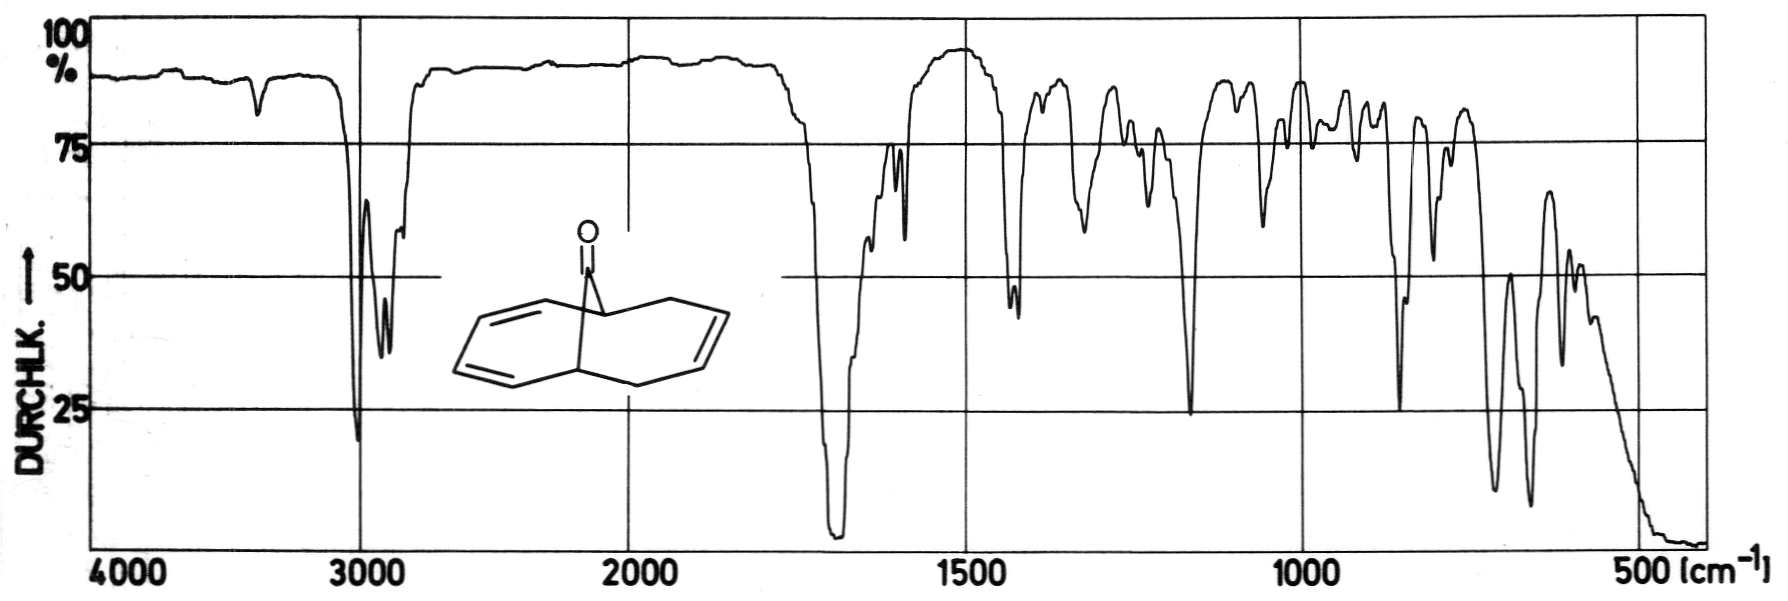
\includegraphics[width=14.38cm]{IR_040}
\begin{alltt}

3025 cm\raise0.5ex\hbox{-1}   =C-H Valenzschwingung
2940 cm\raise0.5ex\hbox{-1}   -C-H Valenzschwingung
2907 cm\raise0.5ex\hbox{-1}
1699 cm\raise0.5ex\hbox{-1}   -C=O Valenzschwingung
1598 cm\raise0.5ex\hbox{-1}   -C=C-
1444 cm\raise0.5ex\hbox{-1}   -CH2- Deformationsschwingung
1432 cm\raise0.5ex\hbox{-1}
 726 cm\raise0.5ex\hbox{-1}   =C-H


\leavevmode\raise0.5ex\hbox{1}H-NMR-Spektrum (in CDCl\lower0.5ex\hbox{3}/TMS)
\end{alltt}
\hspace*{-0.25cm}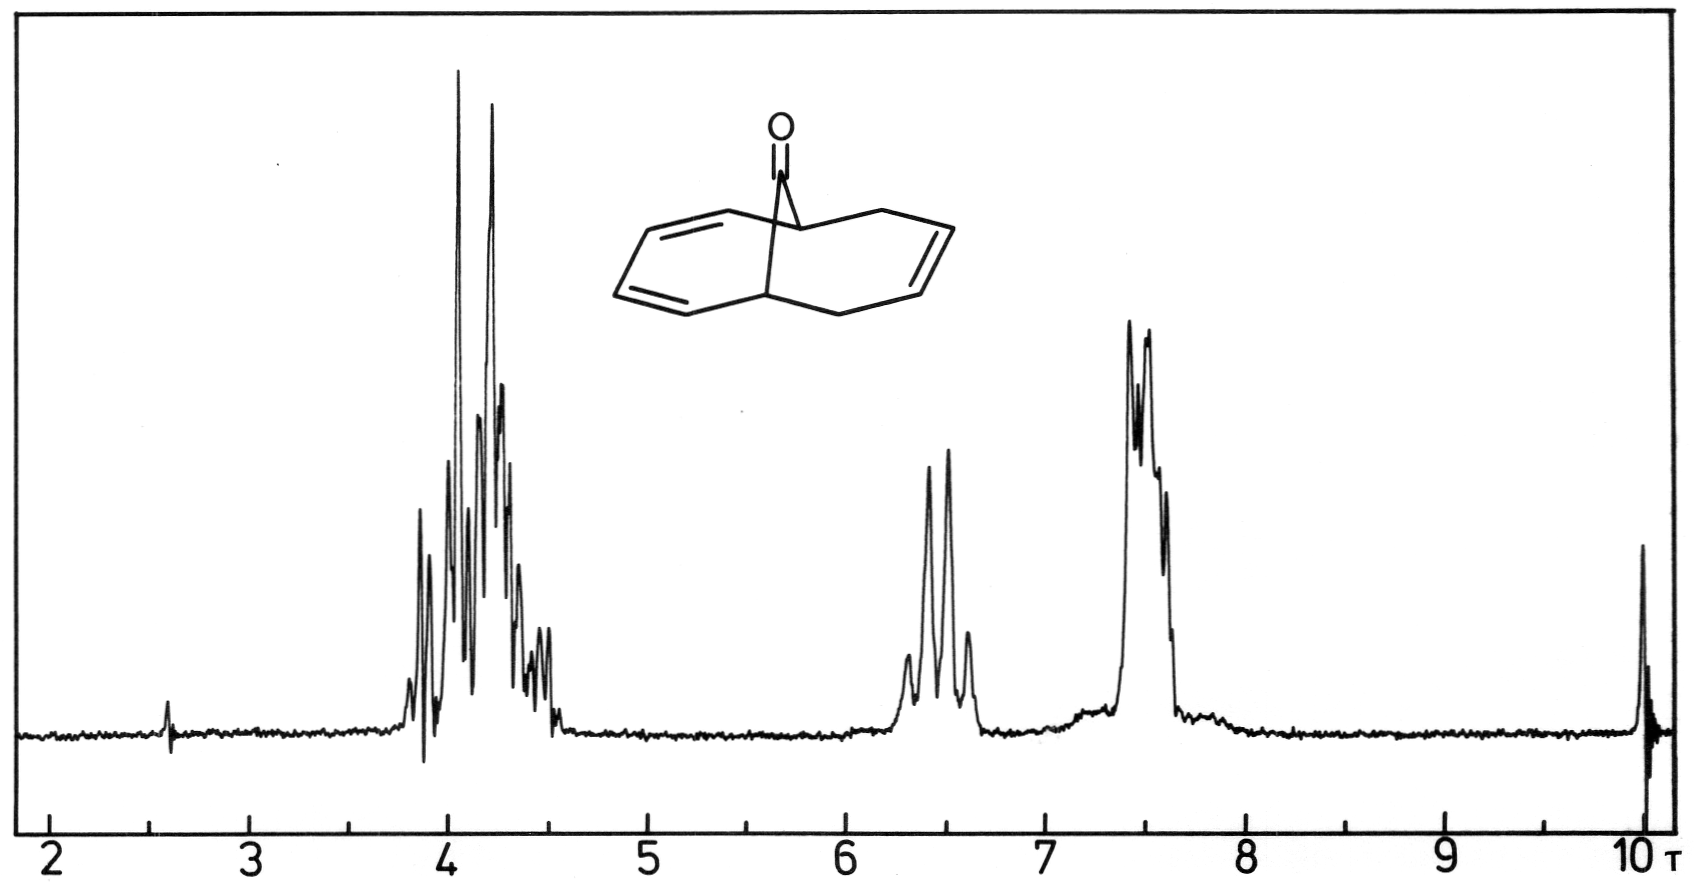
\includegraphics[width=14.38cm]{NMR_041}
\begin{alltt}

  \(\tau\) [ppm]
3.78 - 4.60     Multiplett     6 olefinische Protonen
6.48            Quartett       2 tertiäre Protonen
7.08 - 7.98     Multiplett     4 allylische Protonen

\newpage
\makebox[0.8\textwidth][c]{- 98 -}


Dehydrierung des 11-Oxobicyclo[4.4.1]undecatriens-(2‚4,8) (59)

In einer 100 ml Ampulle werden 1.6 g (0.01 Mol) Cycloadditions-
produkt (59) mit 6.8 g (0.03 Mol) DDCh und 50 ml Benzol 24 h auf
120\degree{}C erhitzt. Nach dem Abkühlen gibt man den gesamten Ampullen-
inhalt auf Säule 6 und eluiert mit Methylenchlorid. Durch Abziehen
des Eluens erhält man 0.2 g gelben, kristallinen Rückstand, der an
Säule 2 weiter aufgetrennt wird. Mit Methylenchlorid eluiert man
als Hauptfraktion 0.13 g (0.0008 Mol = 8 \% d.Th.) aromatisches
Keton (15) vom Fp = 183 - 184\degree{}C.


4.14 11-\underline{endo}-Brombicyclo[4.4.1]undecatetraen-(1,3,5‚8) (45)

Die gesammelten Mutterlaugen von fünf Dehydrierungsansätzen des
11-Bromtricyclo[4.4.1.0\raise0.5ex\hbox{1,6}]undecadiens-(3,8) (24) mit DDCh werden
im Vakuum eingeengt, und der Rückstand (15 - 16 g) mit Methylen-
chlorid auf 40 - 60 g Aluminiumoxid neutral nach Brockmann aufge-
zogen und auf Säule 5 gegeben. Man eluiert mit Pentan, wobei zum
Auffangen der Fraktionen ein automatischer Fraktionssammler ver-
wendet wird. Man isoliert zwei Komponenten:

1) 11-\underline{endo}-Brombicyclo[4.4.1]undecatetraen-(1,3,5‚8) (45)
   Man erhält 8.0 g Substanz, die nach Umkristallisieren aus
   40 ml Methanol in Form weißer Kristallnadeln (5.3 g; 0.024
   Mol = 5 \% d.Th.) vom Fp = 49\degree{}C anfallen. Aus der Mutterlauge
   werden noch 1.3 g (0.006 Mol; Gesamtausbeute: 6 \% d.Th.)
   Bromid (45) vom Fp = 48 - 49\degree{}C gewonnen.

UV-Spektrum (in Cyclohexan)

\(\lambda\)\lower0.5ex\hbox{max} = 253 nm (e = 4000, Sch.)

\newpage
\makebox[0.8\textwidth][c]{- 99 -}


IR-Spektrum (Schmelze)
\end{alltt}
\hspace*{-0.5cm}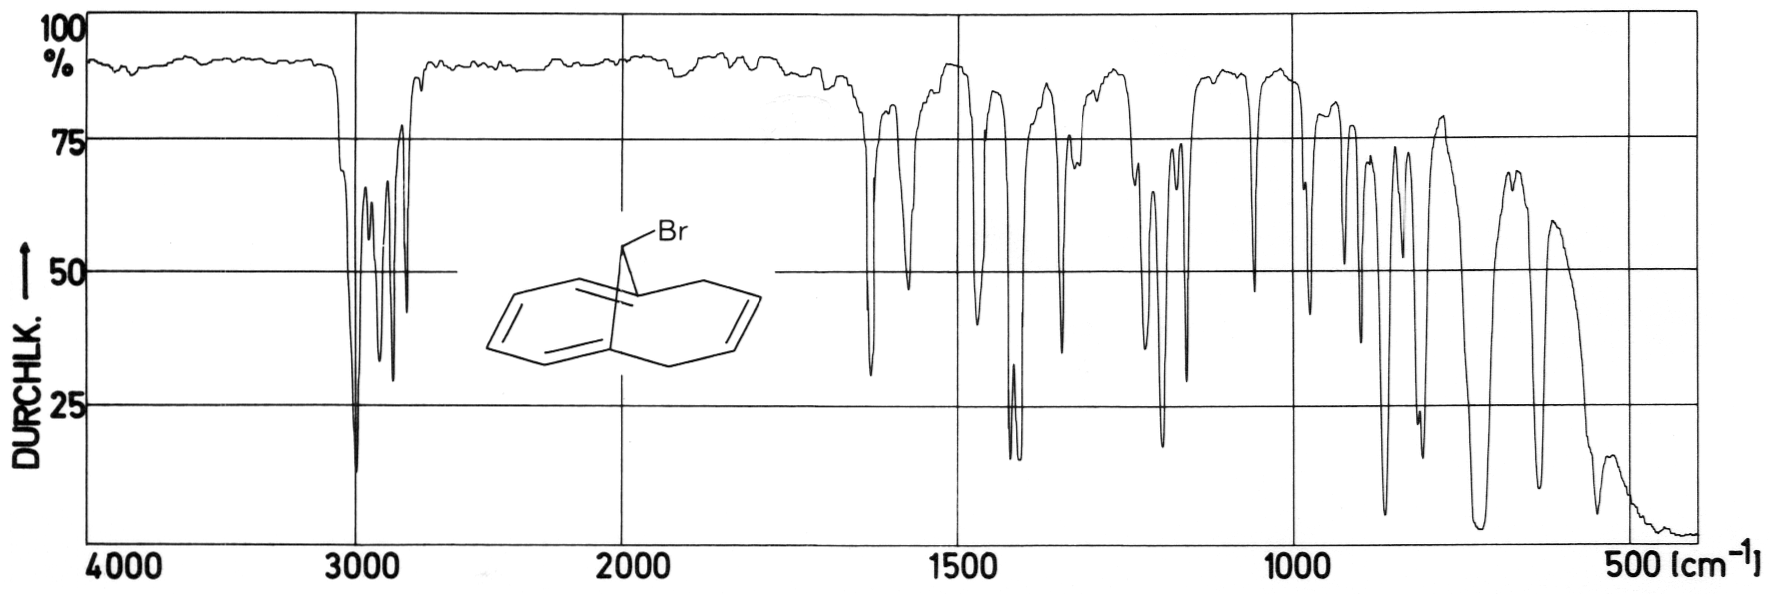
\includegraphics[width=15.07cm]{IR_042}
\begin{alltt}

3020 cm\raise0.5ex\hbox{-1} =C-H Valenzschwingung
2935 cm\raise0.5ex\hbox{-1} -C-H Valenzschwingung
2880 cm\raise0.5ex\hbox{-1}
2830 cm\raise0.5ex\hbox{-1}
1640 cm\raise0.5ex\hbox{-1} -C=C-
1586 cm\raise0.5ex\hbox{-1}
1482 cm\raise0.5ex\hbox{-1} -CH2- Deformationsschwingung
1434 cm\raise0.5ex\hbox{-1}
1420 cm\raise0.5ex\hbox{-1}
 652 cm\raise0.5ex\hbox{-1} -C-Br

\leavevmode\raise0.5ex\hbox{1}H-NMR-Spektrum (in CDCl\lower0.5ex\hbox{3}/TMS) s. Abb. 16 auf S. 40
  \(\tau\) [ppm]
3.02 - 4.30 AA'XX'-System              4 olefinische Protonen
            \(\nu\)\lower0.5ex\hbox{A} = 3.22\(\tau\)
            \(\nu\)\lower0.5ex\hbox{B} = 4.03\(\tau\)
            N = 5.5 Hz
4.35 - 4.73 Multiplett                 2 olefinische Protonen
6.83        Singulett                  1 Brückenproton
6.22 - 7.35 Multiplett mit AB-Charak-  4 allylische Protonen
            ter; J\lower0.5ex\hbox{AB} = 14 Hz


2) 11-Brom-1‚6-methano-[10]annulen (25)
   Es fallen 7.0 g (0.03 Mol = 6 \% d.Th.) Bromid (25) an.

\newpage
\makebox[0.8\textwidth][c]{- 100 -}


4.15 11-\underline{endo}-Acetoxybicyclo[4.4.1]undecatetraen-(1‚3,5,8) (46)

Unter Rückfluss werden 5.7 g (0.03 Mol) Tetraenbromid (45) in 300 ml
Eisessig mit 7.5 g (0.045 Mol) Silber(I)acetat für 24 h erhitzt.
Man lässt abkühlen und gießt nach Filtration in 600 ml Wasser. Das
zur Extraktion verwendete Pentan (5 x 200 ml) wird vorher jeweils
dazu benutzt, die abfiltrierten Silbersalze auszuwaschen. Nach
Waschen mit 5 \%iger Natriumhydrogencarbonat-Lösung und Trocknen
über Magnesiumsultat wird das Lösungsmittel abgezogen und der
weiße kristalline Rückstand (5.4 g) aus 50 ml Petroläther (40-60)
umkristallisiert, wobei 3.8 g (0.019 Mol = 63 \% d.Th.] Kristall-
nadeln vom Fp = 85 - 86\degree{}C resultieren.
0.45 g Acetat (46) werden aus 5 ml Petroläther umkristallisiert.
Das anfallende Produkt (0.3 g = 67 \% Ausbeute) schmilzt bei
85 - 87\degree{}C. Durch nochmaliges Umkristallisieren wird Schmelzpunkts-
konstanz bei 86 - 87\degree{}C erreicht.

Elementaranalyse
C13H14O2 ber.   C  77.20  H  6.98
202.255  gef.      77.06     7.06


IR-Spektrum (4000-520 cm\raise0.5ex\hbox{-1} in CCl\lower0.5ex\hbox{4}, 520-500 cm\raise0.5ex\hbox{-1} in CS\lower0.5ex\hbox{2})
\end{alltt}
\hspace*{-0.5cm}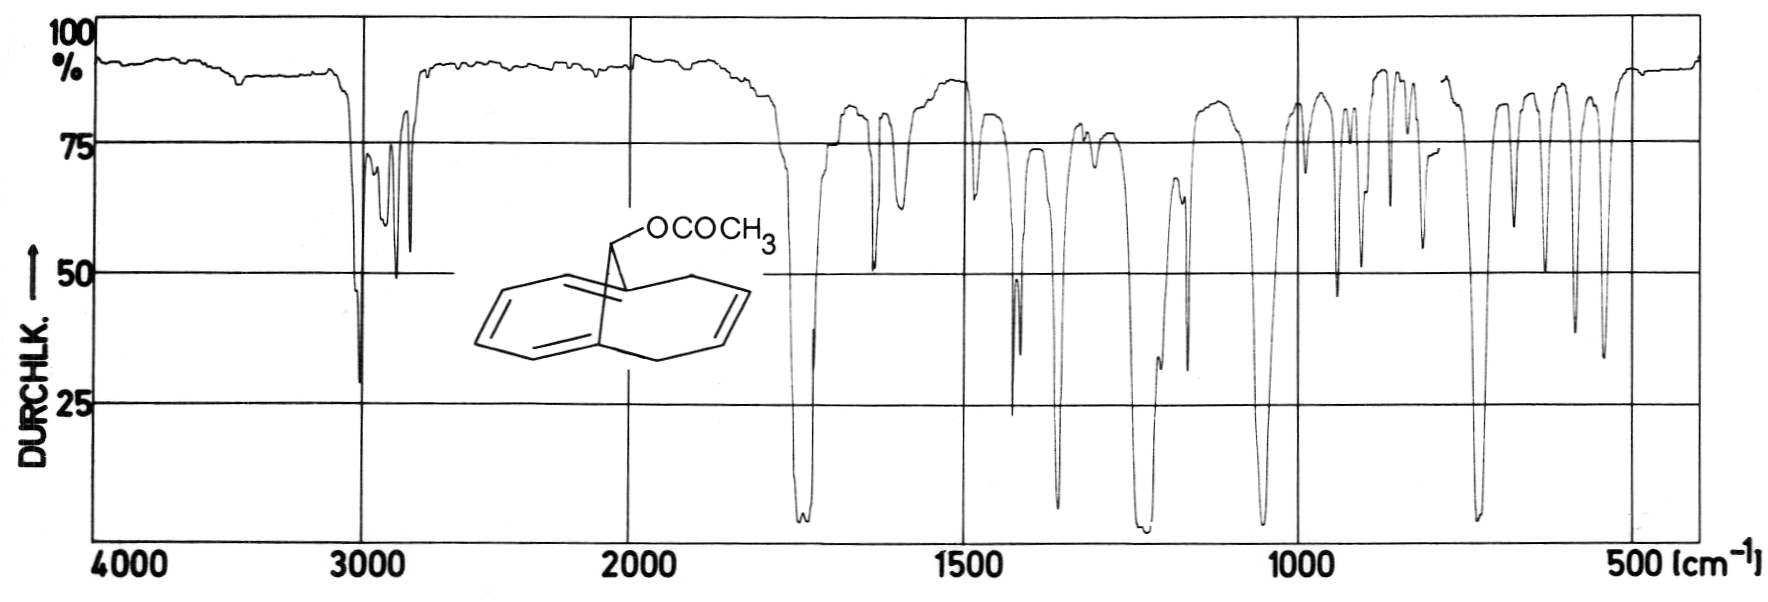
\includegraphics[width=14.97cm]{IR_043}
\begin{alltt}

8030 cm\raise0.5ex\hbox{-1} =C-H Valenzschwingung
2940 cm\raise0.5ex\hbox{-1} -C-H Valenzschwingung
2595 cm\raise0.5ex\hbox{-1}
2840 cm\raise0.5ex\hbox{-1}

\newpage
\makebox[0.8\textwidth][c]{- 101 -}


1756 cm\raise0.5ex\hbox{-1} -C=O Valenzschwingung
1742 cm\raise0.5ex\hbox{-1}
1646 cm\raise0.5ex\hbox{-1} -C=C-
1606 cm\raise0.5ex\hbox{-1}
1438 cm\raise0.5ex\hbox{-1} -CH2- Deformationsschwingung
1240 cm\raise0.5ex\hbox{-1} -C-O Valenzschwingung
1064 cm\raise0.5ex\hbox{-1}
 750 cm\raise0.5ex\hbox{-1} =C-H

UV-Spektrum (in Cyolohexan)

\(\lambda\)\lower0.5ex\hbox{max} = 252 nm (s = 4400)


\leavevmode\raise0.5ex\hbox{1}H-NMR-Spektrum (in CCl\lower0.5ex\hbox{4}/TMS) s. Abb. 17 auf S. 41
  \(\tau\) [ppm]
3.08 - 4.27 AA'XX‘-System                4 Trienprotonen
            \(\nu\)\lower0.5ex\hbox{A} = 3.23\(\tau\)
            \(\nu\)\lower0.5ex\hbox{X} = 4.15\(\tau\)
            N = 5.5 Hz
4.43 - 4.68 Multiplett                   2 olefinische Protonen
6.45        Singulett                    1 Brückenproton
6.57 - 7.45 Multiplett mit AB-Charakter  4 allylische Protonen
7.99        Singulett 3 Methylprotonen


4.46 11-\underline{endo}-Hydroxybicyclo[4.4.1]undecatetraen-(1‚3,5,8) (47)

Man bereitet aus 2.9 g (0.12 Mol) Magnesium, 17.0 g (0.12 Mol)
Methyljodid und 200 ml abs. Äther die GRIGNARD-Verbindung. Bei 0\degree{}C
gibt man innerhalb 10 min 4.0 g (0.02 Mol) Acetat (46) in fester
Form zu und rührt 1 h bei 0\degree{}C sowie 1 h bei Raumtemperatur, wobei
Magnesiumsalze ausfallen. Man kühlt in Eiswasser und versetzt
tropfenweise mit gesättigter Ammoniumchloridlösung. Nach Zersetzung
der überschüssigen GRIGNARD-Verbindung kann der Rest der Lösung
(insgesamt 120 ml) schnell zugegeben werden. Nach Zugabe von 120 ml

\newpage
\makebox[0.8\textwidth][c]{- 102 -}


Äther trennt man die Phasen und wäscht mit 60 ml Ammoniumehlorid-
lösung und 60 ml Wasser. Entfernung des Lösungsmittels nach Trock-
nen über Magnesiumsulfat ergibt 3.2 g weißen Rückstand, der in
50 ml Äther gelöst und mit 40 ml Hexan versetzt wird. Beim Abküh-
len auf -20\degree{}C scheiden sich 2.2 g (0.014 Mal = 69 \% d.Th.) quader-
förmige Kristalle vom Fp = 124 - 127\degree{}C ab.
Umkristallisieren von 0.3 g Alkohol (47) aus 4 ml Äther und 3 ml
Hexan führt zu 0.18 g (60 \% Ausbeute) Kristallen mit Fp = 126 -
127\degree{}C.

Elementaranalyse
C11H12O ber. C  82.46   H  7.55
160.218 gef.    82.06      7.76

IR-Spektrum (in Kaliumbremid)
\end{alltt}
\hspace*{-0.5cm}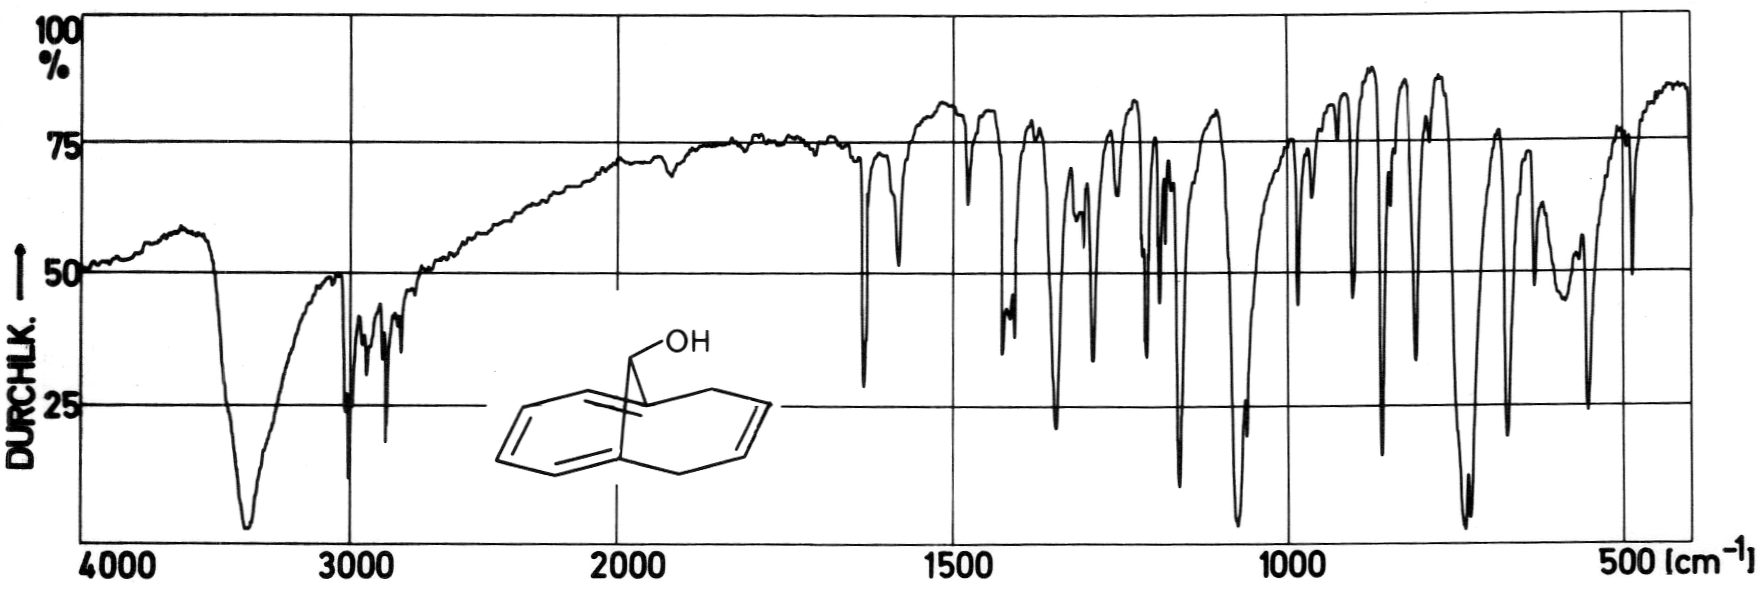
\includegraphics[width=14.92cm]{IR_044}
\begin{alltt}

3390 cm\raise0.5ex\hbox{-1} -O-H Valenzschwingung
302D cm\raise0.5ex\hbox{-1} =C-H Valenzschwingung
2955 cm\raise0.5ex\hbox{-1} -C-H Valenzschwingung
2880 cm\raise0.5ex\hbox{-1}
164D cm\raise0.5ex\hbox{-1} -C=C-
1592 cm\raise0.5ex\hbox{-1}
1490 cm\raise0.5ex\hbox{-1} -CH2- Deformationsschwingung
1436 cm\raise0.5ex\hbox{-1}
1418 cm\raise0.5ex\hbox{-1}
1084 cm\raise0.5ex\hbox{-1} -C-O Valenzschwingung
 748 cm\raise0.5ex\hbox{-1} =C-H

\newpage
\makebox[0.8\textwidth][c]{- 103 -}


UV-Spektrum (in Cyclohexan)

\(\lambda\)\lower0.5ex\hbox{max} = 253 nm (\(\epsilon\) = 3800)


\leavevmode\raise0.5ex\hbox{1}H-NMR-Spektrum (in CDCl\lower0.5ex\hbox{3}/TM5) s. Abb. 18 auf S. 43
  \(\tau\) [ppm]
2.98 - 4.27 AA'XX‘-System                4 Trienprotonen
            \(\nu\)\lower0.5ex\hbox{A} = 3.23\(\tau\)
            \(\nu\)\lower0.5ex\hbox{X} = 4.10\(\tau\)
            N = 5.5 Hz
4.27 - 4.72 Multiplett                   2 olefinische Protonen
6.28 - 7.52 Multiplett mit AB-Charakter  4 allylische Protonen
7.35 Singulett (breit)                   1 Brückenproton und
                                         1 Alkoholproton

4.17 11-Oxobicyclo[4.4.1]undecatetraen-(1‚3,5,8) (14)

Zu einer Mischung von 25 ml Benzol, 1.0 g (0.005 Mol) PTFA, 5.7 g
(0.03 Mol) Äthyl-[3-(dimethylamino)propyl]carbodiimid-hydrochlorid
und 25 ml DMSO fügt man 1.6 g (0.01 Mol) Alkohol (47) in fester
Form zu. Unter leichter Wärmeentwicklung klärt sich die schaumige
Suspension zu einer hellgelben Lösung. Man lässt 36 h bei Raumtempe-
ratur rühren, wobei man jeweils nach 5 h, 15 h und 30 h 0.05 g
(0.00025 Mal) PTFA zusetzt. Nach Zugabe von je 100 ml Äther und
Wasser trennt man die Phasen und extrahiert mit weiteren 100 ml
Äther. Man wäscht mit 4 x 50 ml Wasser, trocknet über Magnesiumsul-
fat und entfernt das Lösungsmittel im Vakuum. Der resultierende
weiße kristalline Rückstand (1.6 g) wird in 15 ml Äther gelöst,
filtriert und mit 10 ml Hexan versetzt. Bei -20\degree{}C kristallisieren
1.1 g (0.007 Mol = 70 \% d.Th.) weiße Kristallblättchen vom Fp =
93 - 95\degree{}C.
Umkristallisieren von 0.2 g Keton (14) ergibt 0.14 g (70 \% Ausbeu-
te) Kristalle mit Fp = 94 - 95.5\degree{}C.

\newpage
\makebox[0.8\textwidth][c]{- 104 -}


Elementaranalyse

C11H10O   ber. C  83.52    H  6.37
158.202   gef.    84.02       6.41

IR-Spektrum (4000-820 cm\raise0.5ex\hbox{-1} in CCl\lower0.5ex\hbox{4}, 820-500 cm\raise0.5ex\hbox{-1} in CS\lower0.5ex\hbox{2})
\end{alltt}
\hspace*{-0.5cm}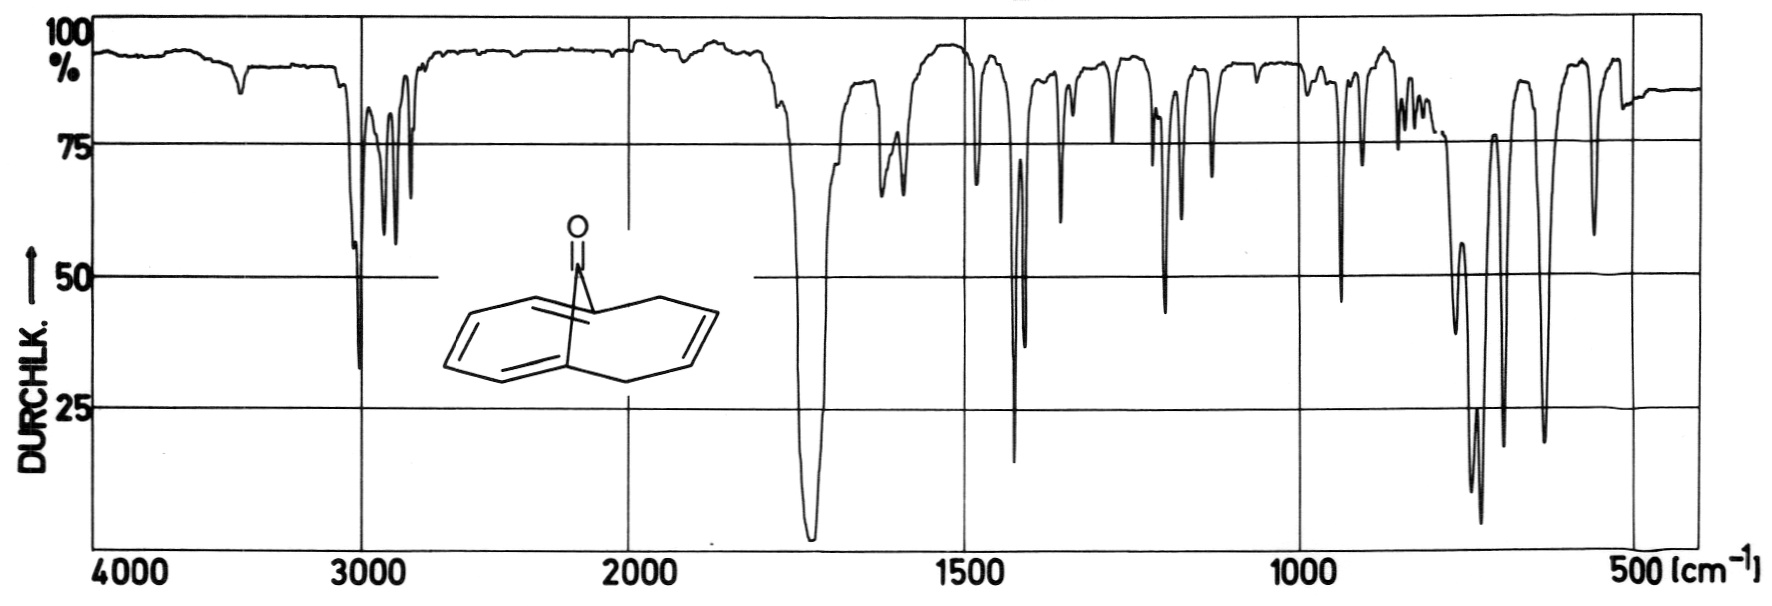
\includegraphics[width=15.0cm]{IR_045}
\begin{alltt}

3020 cm\raise0.5ex\hbox{-1} =C-H Valenzschwingung
2925 cm\raise0.5ex\hbox{-1} -C-H Valenzschwingung
2880 cm\raise0.5ex\hbox{-1}
2830 cm\raise0.5ex\hbox{-1}
174D cm\raise0.5ex\hbox{-1} -C=O Valenzschwingung
1632 cm\raise0.5ex\hbox{-1} -C=C-
1598 cm\raise0.5ex\hbox{-1}
1492 cm\raise0.5ex\hbox{-1} -CH2- Deformationsschwingung
1436 cm\raise0.5ex\hbox{-1}
1420 cm\raise0.5ex\hbox{-1}


UV-Spektrum (in Cyclohexan) s. Abb. 29 auf S. 60

\(\lambda\)\lower0.5ex\hbox{max} = 235 (\(\epsilon\) = 5600) und 251 nm (5800)


\leavevmode\raise0.5ex\hbox{1}H-NMR-Spektrum (in CDCl\lower0.5ex\hbox{3}/TMS, 60 MHz) s. Abb. 21 auf S. 47
\(\tau\) [ppm]
3.00 - 4.02   AA'XX'-System          4 Trienprotonen
              \(\nu\)\lower0.5ex\hbox{A} = 3.23\(\tau\)
              \(\nu\)\lower0.5ex\hbox{X} = 3.77\(\tau\)Lock
              N = 6.0 Hz

\newpage
\makebox[0.8\textwidth][c]{- 105 -}


  \(\tau\) [ppm]
4.12 - 4.73   Multiplett                    2 olefinische Protonen
6.32 - 7.48   Multiplett mit AB-Charakter   4 allylische Protonen


\leavevmode\raise0.5ex\hbox{1}H-NMR-Spektrum (in CD\lower0.5ex\hbox{2}Cl\lower0.5ex\hbox{2}, TMS als Lock, 100 MHz)
\end{alltt}
\hspace{3.5cm}
% 11-Oxo- 1,6-methano-undecatetraen-1,3,5,8 (14) mit Atomnummern
\chemfig[atom style={scale=\normalscale}]{%
=_[:60,,,,shrtdbl={0pt}{3.5pt}]@{n3}%9
-[:12]@{n2}%10
=_[:-12]@{n1}%1
(-[:-252]?@{n11}(=[:90,0.6]O))% 1,6 Brücke
-[:12]@{n10}%2
-[:-12]@{n9}%3
=_[:-120,,,,shrtdbl={0pt}{3.5pt}]@{n8}%4
-[:-168]@{n7}%5
-[:168]?@{n6}%6
=_[:-168,,,,shrtdbl={1pt}{1pt}]@{n5}%7
-[:168]@{n4}%8
}%
\chemmove{
    \node at (n1) [above right=-0.05 and -0.1] {\scriptsize\textsf{1}};
    \node at (n2) [above=-0.05] {\scriptsize\textsf{2}};
    \node at (n3) [left=0] {\scriptsize\textsf{3}};
    \node at (n4) [left=-0.05] {\scriptsize\textsf{4}};
    \node at (n5) [below=-0.05] {\scriptsize\textsf{5}};
    \node at (n6) [below=-0.05] {\scriptsize\textsf{6}};
    \node at (n7) [below=-0.05] {\scriptsize\textsf{7}};
    \node at (n8) [right=0] {\scriptsize\textsf{8}};
    \node at (n9) [right=-0.05] {\scriptsize\textsf{9}};
    \node at (n10) [above=-0.05] {\scriptsize\textsf{10}};
    \node at (n11) [right] {\scriptsize\textsf{11}};
}%
\begin{alltt}

Chemische Verschiebungen:   \(\delta\)(2,5) = 6.769
                            \(\delta\)(3,4) = 6.228
Kopplungskonstanten:        J(2,3) =  5.73 Hz
                            J(2,4) =  0.02 Hz
                            J(2,5) = -0.67 Hz
                            J(3,4) = 11.02 Hz

\leavevmode\raise0.5ex\hbox{13}C-NMR-Spektrum (in CCl\lower0.5ex\hbox{4}/CDCl\lower0.5ex\hbox{3}/TMS) s. Abb. 20 auf S. 46

          \(\delta\) = 125.6         C-1, C-5
          \(\delta\) = 117.9         C-2, C-5
          \(\delta\) = 129.4         C-3, C-4
          \(\delta\) =  30.96        C-7, C-10
          \(\delta\) = 122.8         C-8, C-9
          \(\delta\) = 202.7         C-11

Massenspektrum (100 eV) s. Abb. 19 auf S. 44

m/e       158   (0.6 \%)     M\raise0.5ex\hbox{+}
          157   (1.3 \%)     M\raise0.5ex\hbox{+} - H
          131  (11.6 \%)
          130  (98.9 \%)     M\raise0.5ex\hbox{+} - CO
          129 (100.0 \%)     M\raise0.5ex\hbox{+} - CO - H
          128  (73.7 \%)     M\raise0.5ex\hbox{+} - CO - 2 H
          116   (6.7 \%)     M\raise0.5ex\hbox{+} - CH2CO
          115  (63.9 \%)     M\raise0.5ex\hbox{+} - CH2CO - H

\newpage
\makebox[0.8\textwidth][c]{- 106 -}


11,11-Dimethoxybicyclo[4.4.1]undecatetraen-(1‚3,5,8) (14a)

Man löst 0.8 g (0.005 M01) 11-Oxobicyclo[4.4.1]undecatetraen-
(1,3,5,8) (14a) in 10 ml abs. Methanol und versetzt mit 1.1 g
(0.01 Mol) Orthoameisensäuremethylester und einer Spatelspitze
p-Toluolsulfonsäure. Nach dreitägigem Stehen gibt man festes
Natriumhydrogencarbonat zu, verdünnt mit 25 ml Wasser und extra-
hiert mit 2 x 20 ml Äther. Nach Waschen der organischen Phase
mit 2 x 10 ml Wasser wird über Natriumsulfat getrocknet und das
Lösungsmittel abgezogen. Der Rückstand (0.9 g) wird an Säule 2
(Eluens: Methylenchlorid) chromatographiert, wobei man 0.8 g
farbloses Öl isoliert, das in 5 ml Pentan gelöst wird. Beim Ab-
kühlen auf -20\degree{}C erhält man 0.6 g (0.003 Mol = 59 \% d.Th.) weiße
Kristalle vom Fp = 64 - 66\degree{}C.
Umlösen von 0.2 g Ketal (14a) aus 1 ml Pentan ergibt 0.15 g (75 \%
Wiedergewinnung) weiße Kristalle vom Fp = 66 - 68\degree{}C. Weiteres Um-
kristallisieren führt zur Schmelzpunktskonstanz bei 68 - 69\degree{}C.


IR-Spektrum (4000-820 cm\raise0.5ex\hbox{-1} in CCl\lower0.5ex\hbox{4}, 820-500 cm\raise0.5ex\hbox{-1} in CS\lower0.5ex\hbox{2})
\end{alltt}
\hspace*{-0.3cm}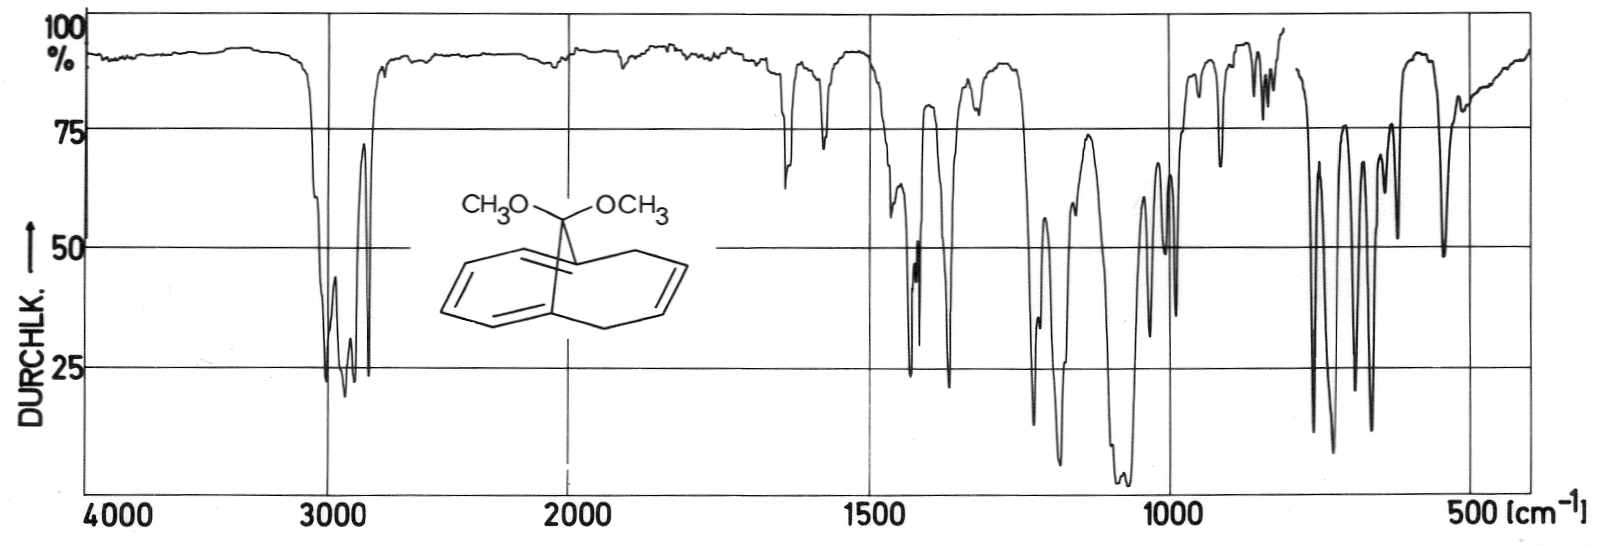
\includegraphics[width=13.53cm]{IR_046}
\begin{alltt}

3075 cm\raise0.5ex\hbox{-1} =C-H Valenzschwingung
3030 cm\raise0.5ex\hbox{-1}
2950 cm\raise0.5ex\hbox{-1} -C-H Valenzschwingung
2915 cm\raise0.5ex\hbox{-1}
2850 cm\raise0.5ex\hbox{-1} -OCH3 Valenzschwingung
1647 cm\raise0.5ex\hbox{-1} -C=C- Streckschwingung
1582 cm\raise0.5ex\hbox{-1}

\newpage
\makebox[0.8\textwidth][c]{- 107 -}


1470 cm\raise0.5ex\hbox{-1} -CH2- Deformationsschwingung
1439 cm\raise0.5ex\hbox{-1}
1373 cm\raise0.5ex\hbox{-1} -CH3  Symm. Deformationsschwingung
1095 cm\raise0.5ex\hbox{-1} -C-O  Valenzschwingung
1075 cm\raise0.5ex\hbox{-1}
 739 cm\raise0.5ex\hbox{-1}       Out-of-Plane-Schwingung


\leavevmode\raise0.5ex\hbox{1}H-NMR-Spektrum (in CCl\lower0.5ex\hbox{4}/TMS)
\end{alltt}
\hspace*{-0.25cm}\includegraphics[width=14.30cm]{NMR_047}
\begin{alltt}

  \(\tau\)[ppm]
3.25 - 4.08  AA'XX'-System                4 olefinische Protonen
\(\nu\)\lower0.5ex\hbox{A} = 3.36\(\tau\)
\(\nu\)\lower0.5ex\hbox{X} = 3.98\(\tau\)
N = 7.5 Hz
4.50 - 4.70  Multiplett                   2 olefinische Protonen
6.62 - 7.73  Multiplett mit AB-Charakter  4 allylische Protonen
J\lower0.5ex\hbox{AB} = 15 HZ
6.65         Singulett                    3 Methylprotonen
7.35         Singulett                    3 Methylprotonen über
                                            dem Trienteil


\newpage
\makebox[0.8\textwidth][c]{- 108 -}


4.18 1‚4,5,6‚7,8-Hexahydronaphthalin (50) \raise0.5ex\hbox{[103]}

Eine Lösung von 132.0 g (1.0 Mol) Tetralin in 500 ml Äther und
233 ml (184 g = 4.0 Mol) Äthanol lässt man unter Rühren bei -78\degree{}C
in 1 l kondensierten Ammoniak laufen und fügt 69.0 g (3.0 Tom)
Natrium in kleinen Stücken zu. Nach 5 h Nachrühren hebt man den
Dreihalskolben aus dem Kühlbad und lässt den Ammoniak über Nacht
verdampfen. Man hydrolysiert unter Schutzgas und Eiskühlung mit
1 l Eiswasser, trennt die organische Phase ab, extrahiert mit
200 ml Äther und trocknet über Magnesiumsulfat. Destillation des
Rückstandes (128 g) nach Abziehen des Lösungsmittels bei 85 - 86\degree{}C
und 16 mm Hg liefert 125.0 g einer farblosen Flüssigkeit, die
laut Gaschromatogramm (Säule A) zu 85 \% aus 1,4-Dihydrotetralin
(50) besteht (79 \% d.Th. Ausbeute).


4.19 11‚11-Dibromtricyclo[4.4.1.0\raise0.5ex\hbox{1,6}]undecen-3 [35]

Zu 158.0 g 85 \%igem (1.0 Mol) 1,4-Dihydrotetralin (50) in 500 ml
Äther gibt man 150 g (ca. 1.3 Mol) Kalium-t-butanolat und tropft
innerhalb 2 - 3 h bei -15\degree bis -10\degree{}C 252.0 g (1.0 Mol) Bromoform
zu. Nach 1 h Nachrühren hydrolysiert man mit 500 ml Wasser, trennt
die ätherische Phase ab und extrahiert mit 2 x 100 ml Äther. Trock-
nen über Magnesiumsulfat und Abziehen des Äthers liefert ein brau-
nes Öl, das im Hochvakuum destilliert wird. Nach einem Vorlauf, der
hauptsächlich aus unumgesetztem 1,4-Dihydrotetralin und Tetralin
besteht, geht bei 115 - 120\degree{}C und 0.2 mm Hg eine farblose Flüssig-
keit (ca. 120 g) über, die in 70 ml Äthylacetat gelöst und auf
-60\degree{}C gekühlt wird. Die sich abscheidenden Kristalle (40 g) werden
aus 250 - 300 ml Methanol (Wasserbad unter 40\degree{}C) umkristallisiert,
wobei man 36.0 g (12 \% d.Th.) weiße Kristallnadeln vom Fp = 44\degree{}C
erhält.


\newpage
\makebox[0.8\textwidth][c]{- 109 -}


4.20 11-Bromtricyclo[4.4.1.0\raise0.5ex\hbox{1,6}]undecaen-3 (52)

Unter Eiskühlung gibt man 61.0 g (0.2 Mol) Dibromcarbenaddukt (51)
und 58.0 g (0.2 Mol) Tri-n-butylzinnhydrid zusammen und erhitzt
nach Abklingen der exothermen Reaktion unter Wasserstrahlvakuum
auf 120 - 130\degree{}C. Nach 5 h wird im Hochvakuum destilliert, wobei
nach einem kleinen Vorlauf (ca. 1.6 g) bei 60 - 78\degree{}C und 0.1 mm Hg
42.0 g (0.19 Mol = 92 \% d.Th.) Bromidgemisch (52) als farbloses Öl
übergehen, das laut \raise0.5ex\hbox{1}H-NMR-Spektrum aus den beiden Isomeren im Ver-
hältnis 3:2 besteht.

Die Trennung der Isomeren erfolgt durch verlustreiche Säulenchro-
matographie:

2.0 g Bromidgemisch (52) werden auf Säule 3 gegeben und mit Pentan
eluiert, wobei Fraktionen zu etwa 20 ml genommen werden. Nach
einem Vorlauf von etwa 150 ml Pentan lässt sich erstmals dünn-
schichtchromatographisch (Al\lower0.5ex\hbox{2}O\lower0.5ex\hbox{3}/Pentan, Jodkammer) Substanz nach-
weisen. Man fängt jetzt noch etwa 10 Fraktionen auf, die jeweils
dünnschichtchromatographisch geprüft werden. Fraktionen gleichen
Inhalts werden vereinigt: Man erhält so neben einer großen Misch-
fraktion zwei Fraktionen, die jeweils nur ein Isomeres enthalten.

1) 11-\underline{endo}-Bromtrioyclo[4.4.1.0\raise0.5ex\hbox{1,6}]undecaen-3 (52a)
Man erhält 0.5 g (25 \% Ausbeute) farbloses Öl.

Elementaranalyse

C11H15Br ber. C 58.17 H 6.66 Br 35.18
227.146  gef.   58.23   6.48    35.42


\newpage
\makebox[0.8\textwidth][c]{- 110 -}


IR-Spektrum (Flüssigkeitsfilm)
\end{alltt}
\hspace*{-0.5cm}\includegraphics[width=14.92cm]{IR_048}
\begin{alltt}

304D cm\raise0.5ex\hbox{-1} =C-H  Valenzschwingung
2935 cm\raise0.5ex\hbox{-1} -C-H  Valenzschwingung
2905 cm\raise0.5ex\hbox{-1}
2880 cm\raise0.5ex\hbox{-1}
284D cm\raise0.5ex\hbox{-1}
1654 cm\raise0.5ex\hbox{-1} -C=C- Streckschwingung
1464 cm\raise0.5ex\hbox{-1} -CH2- Deformationsschwingung
1446 cm\raise0.5ex\hbox{-1}
1430 cm\raise0.5ex\hbox{-1}
 664 cm\raise0.5ex\hbox{-1} -C-Br

\leavevmode\raise0.5ex\hbox{1}H-NMR-Spektrum (in CCl\lower0.5ex\hbox{4}/TMS) s. Abb. 22 auf S. 50
  \(\tau\) [ppm]
4.25 - 4.73  Multiplett                  2 alefinische Protonen
6.72         Singulett                   1 Brückenproton
7.23 - 8.15  Multiplett (AB-System)      4 allylische Protonen
8.15 - 8.98  Multiplett                  8 alicyclische Protonen


2) 11-\underline{exo}-Bromtricyclo[4.4.1.0\raise0.5ex\hbox{1,6}]undecaen-3 (52b)

Es werden 0.1 g (5 \% Ausbeute) farbloses Öl isoliert.

Elementaranalyse

C11H15Br ber. C 58.17 H 6.66 Br 35.18
227.146  geF.   58.15   6.52    35.32

\newpage
 
\makebox[0.8\textwidth][c]{- 111 -}


IR-Spektrum (Flüssigkeitsfilm)
\end{alltt}
\hspace*{-0.5cm}\includegraphics[width=14.95cm]{IR_049}
\begin{alltt}

3040 cm\raise0.5ex\hbox{-1} =C-H Valenzschwingung
2935 cm\raise0.5ex\hbox{-1} -C-H Valenzschwingung
2900 cm\raise0.5ex\hbox{-1}
2870 cm\raise0.5ex\hbox{-1}
2840 cm\raise0.5ex\hbox{-1}
1676 cm\raise0.5ex\hbox{-1} -C=C- Streckschwingung
1464 cm\raise0.5ex\hbox{-1} -CH2- Deformationsschwingung
1448 cm\raise0.5ex\hbox{-1}
1426 cm\raise0.5ex\hbox{-1}
 655 cm\raise0.5ex\hbox{-1} -C-Br


\leavevmode\raise0.5ex\hbox{1}H-NMR-Spektrum (in CCl\lower0.5ex\hbox{4}/TMS) 5. Abb. 22 auf S. 50

  \(\tau\) [ppm]
4,33 - 4.72  Multiplett                 2 olefinische Protonen
7.02         Singulett                  1 Brückenproton
7.80         Singulett (AB-System)      4 allylische Protonen
7.93 - 8.90  Multiplett                 8 alicyclische Protonen


\newpage
\makebox[0.8\textwidth][c]{- 112 -}


4.21 11-Brombicyclo[4.4.1]undecatrien-(1‚3,5) (53)

Dehydrierung mit 2,3-Dichlor-5,6-dicyan-1,4-benzochinon
Man erhitzt 22.7 g (0.1 Mol) rohes Bromidgemisch (52) und 34.0 g
(0.15 Mol) DDCh in 150 ml Dioxan für 3 h auf 120\degree{}C. Man filtriert
über Säule 8 mit Pentan und erhält nach dem Abziehen des Lösungs-
mittels 19.0 g braunes Öl, das laut \raise0.5ex\hbox{1}H-NMR-Spektrum die beiden Iso-
meren im Verhältnis 3:1 enthält. Die Substanz wird mit Methylen-
chlorid auf 50 g Aluminiumoxid neutral nach Brockmann aufgezogen
und anschließend an Säule 3 mit Pentan chromatographiert..Man elu-
iert zwei Fraktionen:

1) 11.0 g (0.049 Mol = 49 \% d.Th.) 11-\underline{endo}-Brombicyclo[4.4.1]un-
decatrien-(1,3‚5) (53a) als farbloses Öl.

2) 4.4 g (0.02 Mol = 20 \% 0.Th.) 11-\underline{exo}-Brombicyclc[4.4.1]undeca-
trien-(1‚3,5) (53b) als weiße Kristalle.

Dehydrierung mit Selendioxid
In 300 ml Dioxan und 30 ml Wasser werden 22.7 g (0.1 Mol) rohes
Bromidgemisch (52) mit 22.2 g (0.2 Mol) Selendioxid und 8.1 g
(0.06 Mol) Kaliumdihydrogenphosphat für 5 h zum Rückfluß erhitzt.
Nach dem Abkühlen verdünnt man mit 500 ml Äther und filtriert vom
ausgeschiedenen Selen ab. Nach Zugabe von 1 1 Wasser trennt man
die Phasen und extrahiert mit 2 x 200 ml Äther. Trocknen über
Magnesiumsulfat und Abziehen des Äthers im Vakuum ergeben ca. 25 g
braunrotes Öl, das an Säule 3 nach Aufziehen auf 60 g Aluminium-
oxid neutral nach Brockmann mit Pentan chromatographiert wird.
Es resultieren zwei Fraktionen:

1) 11-\underline{endo}-Brombicyclo[4.4.1]undecatrien-(1‚3,5) (53a)
Man erhält 10.0 g (0.044 Mol = 45 \% d.Th.) farbloses Öl.
Zur Charakterisierung wird 1.0 g Bromid (53a) bei 75 - 77\degree{}C
und 0.15 mm Hg destilliert (0.9 g = 90 \% Ausbeute).

\newpage
\makebox[0.8\textwidth][c]{- 113 -}


Elementaranalyse
C11H13Br ber. C 58.69 H 5.82 Br 35.49
225.130  gef.   58.68   5.85    35.47

IR-Spektrum (Flüssigkeitsfilm)
\end{alltt}
\hspace*{-0.5cm}\includegraphics[width=14.87cm]{IR_050}
\begin{alltt}

3035 cm\raise0.5ex\hbox{-1} =C-H  Valenzschwingung
3010 cm\raise0.5ex\hbox{-1}
2930 cm\raise0.5ex\hbox{-1} -C-H  Valenzschwingung
2855 cm\raise0.5ex\hbox{-1}
1581 cm\raise0.5ex\hbox{-1} -C=C- Streckschwingung
1480 cm\raise0.5ex\hbox{-1} -CH2- Deformationsschwingung
 742 cm\raise0.5ex\hbox{-1} =C-H
 730 cm\raise0.5ex\hbox{-1}



UV-Spektrum (in Cyclchexan)

\(\lambda\)\lower0.5ex\hbox{max} = 253 nm (\(\epsilon\) = 5500)

\leavevmode\raise0.5ex\hbox{1}H-NMR-Spektrum (in CCl\lower0.5ex\hbox{4}/TMS] s. Abb. 23 auf S. 52
  \(\tau\) [ppm]
3.08 - 4.33  AA'XX'-System    4 olefinische Protonen
             \(\nu\)\lower0.5ex\hbox{A} = 3.33\(\tau\)
             \(\nu\)\lower0.5ex\hbox{B} = 4.13\(\tau\)
             N = 5.5 Hz
6.78         Singulett        1 Brückenproton
6.87 - 8.57  Multiplett       6 alicyclische Protonen
8.62 - 9.43  Multiplett       2 alicyclische Protonen

\newpage
\makebox[0.8\textwidth][c]{- 114 -}


2) 11-\underline{exo}-Brombicyclo[4.4.1]undecatrien-(1‚3,5) (53b)

Es werden 4.5 g (0.02 Mol = 20 \% d.Th.) weiße Kristalle iso-
liert. Zur Reinigung löst man in 35 ml Methanol und lässt bei
-20\degree{}C auskristallisieren, wobei 3.0 g (0.013 Mol = 13 \% d.Th.)
weiße Kristallnadeln vom Fp = 33 - 34\degree{}C anfallen.

Elementaranalyse
C11H13Br ber. C 58.69  H 5.82  Br 35.49
225.130  gef.   58.70    5.86     35.43

IR-Spektrum (4000-820 cm\raise0.5ex\hbox{-1} in CCl\lower0.5ex\hbox{4}, 820-500 cm\raise0.5ex\hbox{-1} in CS\lower0.5ex\hbox{2})
\end{alltt}
\hspace*{-0.5cm}\includegraphics[width=14.85cm]{IR_051}
\begin{alltt}

3045 cm\raise0.5ex\hbox{-1} =C-H Valenzschwingung
3025 cm\raise0.5ex\hbox{-1}
2957 cm\raise0.5ex\hbox{-1} -C-H Valenzschwingung
2860 cm\raise0.5ex\hbox{-1}
1598 cm\raise0.5ex\hbox{-1} -C=C- Streckschwingung
1442 cm\raise0.5ex\hbox{-1} -CH2- Deformationsschwingung
 735 cm\raise0.5ex\hbox{-1} =C-H


UV-Spektrum (in Cyclohexan)

\(\lambda\)\lower0.5ex\hbox{max} = 234 (\(\epsilon\) = 13300), 262 (5800, Sch.) und 305 nm
     (600, Sch.)


\newpage
\makebox[0.8\textwidth][c]{- 115 -}


\leavevmode\raise0.5ex\hbox{1}H-NMR-Spektrum (in CDCl\lower0.5ex\hbox{3}/TMS) s. Abb. 23 auf S. 52
  \(\tau\) [ppm]
2.85 - 4.17  AA'XX'-System      4 olefinische Protonen
             \(\nu\)\lower0.5ex\hbox{A} = 3.08\(\tau\)
             \(\nu\)\lower0.5ex\hbox{B} = 3.92\(\tau\)
             N = 6.5 Hz
4.40         Singulett          1 Brückenproton
6.67 - 9.35  Multiplett         8 alicyclische Protonen


4.22 11-\underline{endo}-Acetoxybicyclo[4.4.1]undecatrien-(1‚3,5) (54)

9.0 g (0.04 Mol) \underline{endo}-Bromid (53a) werden in 400 ml Eisessig mit
10.0 g (0.06 Mol) 5i1ber(I)acetat 24 h bei 120\degree{}C gerührt. Man lässt
abkühlen und filtriert die ausgeschiedenen Silbersalze ab, wobei
man jeweils mit dem zum Ausschütteln bestimmten Pentan nachwäscht.
Die Essiglösung wird mit 800 ml Wasser verdünnt und mit 4 x 300 ml
Pentan extrahiert. Die Pentanlösung wird mit 2 x 300 ml 5 \%iger
Natriumhydrogencarbonat-Lösung gewaschen, über Magnesiumsulfat ge-
trocknet, und das Lösungsmittel im Vakuum abgezogen. Der feste
Rückstand (7.7 g) wird in 40 ml Petroläther (40-60) bei Raumtem-
peratur gelöst. Bei -20\degree{}C kristallisieren 5.4 g (0.026 Mol = 66 \%
d.Th.) weiße Kristallnadeln vom Fp = 54 - 55\degree{}C.

Umkristallisieren von 0.2 g Acetat (54) aus 1 ml Petroläther führt
zu 0.15 g (75 \% Ausbeute) Substanz mit konstantem Schmelzpunkt
bei 55 - 56\degree{}C.

Elementaranalyse
C13H16O2  ber.  C 76.44 H 7.90
204.271   gef.    76.19   7.90

UV-Spektrum (in Cyclohexan)

\(\lambda\)\lower0.5ex\hbox{max} = 252 nm (\(\epsilon\) = 5500)

\newpage
\makebox[0.8\textwidth][c]{- 116 -}


IR-Spektrum (4000-820 cm\raise0.5ex\hbox{-1} in CCl\lower0.5ex\hbox{4}, 820-500 cm\raise0.5ex\hbox{-1} in CS\lower0.5ex\hbox{2})
\end{alltt}
\hspace*{-0.5cm}\includegraphics[width=15.04cm]{IR_052}
\begin{alltt}

3030 cm\raise0.5ex\hbox{-1} =C-H     Valenzschwingung
2935 cm\raise0.5ex\hbox{-1} -C-H     Valenzschwingung
2835 cm\raise0.5ex\hbox{-1}
1752 cm\raise0.5ex\hbox{-1} -C=O     Valenzschwingung
1598 cm\raise0.5ex\hbox{-1} -C=C-    Streckschwingung
1444 cm\raise0.5ex\hbox{-1} -CH2-    Deformationsschwingung
1440 cm\raise0.5ex\hbox{-1}
1366 cm\raise0.5ex\hbox{-1} O-CO-CH3
1236 cm\raise0.5ex\hbox{-1} -C-O     Valenzschwingung
 738 cm\raise0.5ex\hbox{-1} =C-H

\leavevmode\raise0.5ex\hbox{1}H-NMR-Spektrum (in CCl\lower0.5ex\hbox{4}/TMS) s. Abb. 24 auf S. 54
  \(\tau\) [ppm]
3.22 - 4.37  AA'XX'-System           4 olefinische Protonen
             \(\nu\)\lower0.5ex\hbox{A} = 3.32\(\tau\)
             \(\nu\)\lower0.5ex\hbox{X} = 4.20\(\tau\)
             N = 5.5 Hz
6.38         Singulett               1 Brückenproton
7.93         Singulett               3 Methylprotanen
7.13 - 9.35  Multiplett              8 alicyclische Protonen

\newpage
\makebox[0.8\textwidth][c]{- 117 -}


4.23 11-\underline{endo}-Hydroxybicyclo[4.4.1]undecatrien-(1‚3,5) (55)

Aus 2.9 g (0.12 Mol) Magnesiumspänen, 17.0 g (0.12 Mol) Methyl-
jodid und 200 ml Äther bereitet man die GRIGNARD-Verbindung, wo-
nach man bei 0\degree{}C innerhalb 10 min 4.1 g (0.02 Mol) Acetat (54)
zugibt. Nach 10 min entfernt man das Eisbad und lässt 2 h bei
Raumtemperatur rühren, wobei Magnesiumsalze ausfallen. Es wird
auf 0\degree{}C gekühlt und tropfenweise mit gesättigter Ammoniumchlorid-
Lösung versetzt, bis die überschüssige GRIGNARD-Verbindung zer-
setzt ist. Danach kann der Rest der Ammoniumchlorid-Lösung (ins-
gesamt 120 ml) schnell zugegeben werden. Man gibt 120 ml Äther
zu und trennt die wässrige Phase ab. Die Ätherlösung wird mit
60 ml Ammoniumchlorid-Lösung sowie 60 ml Wasser gewaschen und
über Natriumsulfat getrocknet. Abziehen des Lösungsmittels im
Vakuum ergibt 3.4 g weißen festen Rückstand, der bei Raumtempe-
ratur in 5 ml Äther aufgenommen und mit 5 ml Hexan versetzt wird.
Durch kurzes Frieren auf - 78\degree{}C werden Impfkristalle erzeugt, da-
nach lässt man bei -20\degree{}C auskristallisieren. Es resultieren 1.5 g
(0.009 Mol = 46 \% d.Th.) rhombische weiße Kristalle vom Schmelz-
punkt 68 - 72\degree{}C.

Verlustreiches dreimaliges Umkristallisieren aus Äther/Hexan
führt zur Schmelzpunktskonstanz bei 72 - 73\degree{}C.

IR-Spektrum (in Kaliumbromid)
\end{alltt}
\hspace*{-0.5cm}\includegraphics[width=15.43cm]{IR_053}
\begin{alltt}

3265 cm\raise0.5ex\hbox{-1} -C-H Valenzschwingung
3020 cm\raise0.5ex\hbox{-1} =C-H Valenzschwingung


\newpage
\makebox[0.8\textwidth][c]{- 118 -}


2925 cm\raise0.5ex\hbox{-1} -C-H Valenzschwingung
2850 cm\raise0.5ex\hbox{-1}
1592 cm\raise0.5ex\hbox{-1} -C=C- Streckschwingung
1492 cm\raise0.5ex\hbox{-1} -CH2- Deformationsschwingung
1436 cm\raise0.5ex\hbox{-1}
1076 cm\raise0.5ex\hbox{-1} -C-O Valenzschwingung
 736 cm\raise0.5ex\hbox{-1} =C-H

UV-Spektrum (in Cyclohexan)

\(\lambda\)\lower0.5ex\hbox{max} = 255 nm (\(\epsilon\) = 5200)

\leavevmode\raise0.5ex\hbox{1}H-NMR-Spektrum (in CDCl\lower0.5ex\hbox{3}/TMS) s. Abb. 25 auf S. 56

  \(\tau\) [ppm]
3.08 - 4.42   AA'XX’-System    4 olefinische Protonen
              \(\nu\)\lower0.5ex\hbox{A} = 3.32 \(\tau\)
              \(\nu\)\lower0.5ex\hbox{X} = 4.17 \(\tau\)
              N = 5.5 Hz
7.25          Singulett        1 Brückenproton
7.35          Singulett        1 Alkoholproton
6.95 - 7.55   Multiplett       2 alicyclische Protonen
7.55 - 8.57   Multiplett       4 alicyclische Protonen
8.62 - 9.43   Multiplett       2 alicyclische Protonen


4.24 11-Oxobicyclo[4‚4‚1]undecatrien-(1‚3,5) (13)

Man löst 1.0 g (0.005 Mol) PTFA und 5.7 g (0.03 M51) Äthyl-
[3-(dimethylamino)propyl]carbodiimid-hydrochlorid in 25 ml Benzol
und 25 ml DMSO und fügt 1.6 g (0.01 Mol) Alkohol (55) hinzu. Die
schaumige Suspension klärt sich innerhalb 10 min unter leichter
Wärmeentwicklung zu einer hellgelben Lösung, die nach 24 h Rühren
dunkelgelb geworden ist und intensiv nach Dimethylsulfid riecht.
Dünnschichtchrometographisch (SiO\lower0.5ex\hbox{2}/CH\lower0.5ex\hbox{2}Cl\lower0.5ex\hbox{2}) ist zu diesem Zeitpunkt
kein Edukt (55) mehr festzustellen. Man verdünnt mit 100 ml Äther


\newpage
\makebox[0.8\textwidth][c]{- 119 -}


und 100 ml Wasser. Nach Trennen der Phasen wird nochmals mit 50 ml
Äther extrahiert. Man wäscht die organische Phase mit 4 x 50 ml
Wasser, trocknet über Magnesiumsulfat und zieht das Lösungsmittel
im Vakuum ab. Das hinterbleibende weiße Kristallpulver (1.5 g)
wird in 8 ml Äther gelöst, filtriert und mit 2 ml Hexen versetzt.
Bei -20\degree{}C kristallisieren 1.2 g (0.0075 Mol = 75 \% d.Th.) farblose
Nadeln vom Fp = 62.5 - 64\degree{}C.
0.2 g Keton (13) werden aus 1 ml Äther und wenig Hexan umkristalli-
siert, wobei 0.15 g (75 \% Ausbeute) Kristalle vom konstanten
Fp = 63 - 65\degree{}C resultieren.

Elementaranalyse
C11H12O ber. C 82.46 H 7.55
160.218 geF.   82.29   7.70

IR-Spektrum (4000-820 cm\raise0.5ex\hbox{-1} in CCl\lower0.5ex\hbox{4}, 820-500 cm in CS\lower0.5ex\hbox{2})
\end{alltt}
\hspace*{-0.5cm}\includegraphics[width=15.0cm]{IR_054}
\begin{alltt}

3050 cm\raise0.5ex\hbox{-1}  =C-H   Valenzschwingung
3025 cm\raise0.5ex\hbox{-1}
2945 cm\raise0.5ex\hbox{-1}  -C-H   Valenzschwingung
2862 cm\raise0.5ex\hbox{-1}
1729 cm\raise0.5ex\hbox{-1}  -C=O   Valenzschwingung
1602 cm\raise0.5ex\hbox{-1}  -C=C-  Streckschwingung
1454 cm\raise0.5ex\hbox{-1}  -CH2-  Deformationsschwingung
1440 cm\raise0.5ex\hbox{-1}
 740 cm\raise0.5ex\hbox{-1}  =C-H


\newpage
\makebox[0.8\textwidth][c]{- 120 -}


UV-Spektrum (in Cyclohexan) s. Abb. 29 auf S. 50

\(\lambda\)\lower0.5ex\hbox{max} = 237 (\(\epsilon\) = 6800) und 247 nm (6600)


\leavevmode\raise0.5ex\hbox{1}H-NMR-Spektrum (in CDCl\lower0.5ex\hbox{3}/TMS) 5. Abb. 27 auf S. 59
  \(\tau\) [ppm]
3.12 - 4.05   AA'XX'-System    4 oleFinische Protonen
              \(\nu\)\lower0.5ex\hbox{A} = 3.33 \(\tau\)
              \(\nu\)\lower0.5ex\hbox{X} = 3.83 \(\tau\)
              N = 6.0 Hz
7.05 _ 9.17   Multiplett       8 alicyclische Protonen

\leavevmode\raise0.5ex\hbox{13}C-NMR-Spektrum (in CCl\lower0.5ex\hbox{4}/CDCl\lower0.5ex\hbox{3}/TMS) s. Abb. 28 auf S. 59
\end{alltt}
\hspace{3.5cm}
% 11-Oxo- 1,6-methano-undecatrien (13) mit Atomnummern
\chemfig[atom style={scale=\normalscale}]{%
=_[:60,,,,shrtdbl={0pt}{3.5pt}]@{n3}%9
-[:12]@{n2}%10
=_[:-12]@{n1}%1
(-[:-252]?@{n11}(=[:90,0.6]O))% 1,6 Brücke
-[:12]@{n10}%2
-[:-12]@{n9}%3
-[:-120]@{n8}%4
-[:-168]@{n7}%5
-[:168]?@{n6}%6
=_[:-168,,,,shrtdbl={1pt}{1pt}]@{n5}%7
-[:168]@{n4}%8
}%
\chemmove{
    \node at (n1) [above right=-0.05 and -0.1] {\scriptsize\textsf{1}};
    \node at (n2) [above=-0.05] {\scriptsize\textsf{2}};
    \node at (n3) [left=0] {\scriptsize\textsf{3}};
    \node at (n4) [left=-0.05] {\scriptsize\textsf{4}};
    \node at (n5) [below=-0.05] {\scriptsize\textsf{5}};
    \node at (n6) [below=-0.05] {\scriptsize\textsf{6}};
    \node at (n7) [below=-0.05] {\scriptsize\textsf{7}};
    \node at (n8) [right=0] {\scriptsize\textsf{8}};
    \node at (n9) [right=-0.05] {\scriptsize\textsf{9}};
    \node at (n10) [above=-0.05] {\scriptsize\textsf{10}};
    \node at (n11) [right] {\scriptsize\textsf{11}};
}%
\begin{alltt}
          \(\delta\) = 133.0          C-1, C-6
          \(\delta\) = 118.0          C-2, C-5
          \(\delta\) = 128.7          C-3, C-4
          \(\delta\) =  29.23         C-7, C-10
          \(\delta\) =  25.73         C-8, C-9
          \(\delta\) = 202.1          C-11


Massenspektrum (100 eV) s. Abb. 26 auf 5. 57

m/e
          160   (0.5 \%)      M\raise0.5ex\hbox{+}
          159   (0.5 \%)      M\raise0.5ex\hbox{+} - H
          132   (5.0 \%)      M\raise0.5ex\hbox{+} - CO
          131  (43.3 \%)      M\raise0.5ex\hbox{+} - CO - H
          130  (14.1 \%)      M\raise0.5ex\hbox{+} - CO - H2
          128   (4.6 \%)      M\raise0.5ex\hbox{+} - CO - 2 H2
          117  (16.1 \%)      M\raise0.5ex\hbox{+} - CH2CO - H
          115  (14.6 \%)      M\raise0.5ex\hbox{+} - CH2COO - H2 - H
          104 (100.0 \%)      M\raise0.5ex\hbox{+} - C4H8

\newpage
\makebox[0.8\textwidth][c]{- 121 -}


4.25 11-Oxo-3’‚6',3,4,9,10-hexahydro-1,2-benzo-4,9-methano-
     [10]annulen (64)

3,6-Dihydrophthalylalkohol \raise0.5ex\hbox{[122]}
Man kocht 26.6 g (0.7 Mol) Lithiumalanat in 600 ml abs. THF für
30 min, kühlt auf 0\degree{}C und lässt unter Argon innerhalb 3 - 5 h 117.7 g
(0.6 Mol) 3,6-Dihydrophthalsäuredimethylester in 1 l abs. THF zu-
tropfen. Es wird über Nacht bei Raumtemperatur nachgerührt, wonach
bei -20\degree{}C mit 50 ml (2.8 Mol) Wasser hydrolysiert wird. Der Alumi-
niumhydroxid-Niederschlag wird abgesaugt, in 1 l gesättigter Seig-
nettesalz-Lösung aufgenommen und mit 2 x 400 ml Äther extrahiert.
Die organische Phase wird mit dem Filtrat vereinigt, über Magnesium-
sulfat getrocknet und am Rotationsverdampfer abgezogen. Der Rück-
stand (ca. 60 g) wird im Hochvakuum bei 110 - 130\degree{}C und 0.2 mm Hg
destilliert, wobei 44.2 g (0.32 Mol = 52.5 \% d.Th.) fast farbloses
viskoses Öl resultieren.

3,6-Dihydrophthalylbromid \leavevmode\raise0.5ex\hbox{*})
Unter Erwärmen werden 30.8 g (0.22 Mol) Dihydrophthalylalkohol in
300 ml abs. Äther gelöst und mit 11.6 g (0.15 Mol) Pyridin versetzt.
In einer Argonatmosphäre wird bei 0\degree{}C unter Rühren eine Lösung von
40.8 g (0.15 Mol) frisch destilliertem Phosphortribromid (Kp = 51\degree{}C
bei 12 mm Hg) in 50 ml abs. Äther zugetropft. Man rührt 1 h bei 0\degree{}C
und 12 h bei Raumtemperatur, gießt die Reaktionsmischung in 250 ml
argongesättigtes Eiswasser und extrahiert mit 3 x 50 ml argonge-
sättigtem Äther. Man wäscht mit 2 x 50 ml eiskalter, argongesättig-
ter Natriumhydrogencarbonat-Lösung und 3 x 50 ml Eiswasser. Nach
Trocknen über Magnesiumsulfat und Abziehen des Lösungsmittels hin-
terbleiben 31.6 g (0.12 Mol = 54 \% d.Th.) schwach gelbe Kristalle.


\(\overline{\hspace{7cm}}\)
\leavevmode\raise0.5ex\hbox{*}) Das entstehende 3,6-Dihydrophthalylbromid ist haut- und augen-
   reizend. Alle Operationen sollten daher im Abzug vorgenommen
   werden. Beim Ausschütteln empfiehlt es sich, Gummihandschuhe zu
   tragen.


\newpage
\makebox[0.8\textwidth][c]{- 122 -}


1‚6-Dimethylencyclohexen-3

Innerhalb von 2 - 3 h tropft man unter Eiskühlen und Argondurch-
leiten zu einer Suspension von 59.0 g (0.9 Mol) Zinkpulver in
300 ml abs. DMF eine Lösung von 31.6 g (0.12 Mol) Dihydrophthalyl-
bromid in 190 ml abs. DMF und lässt noch 3 h bei Raumtemperatur
nachrühren, wonach laut Dünnschichtchromatogramm (SiO2/Pentan)
kein Edukt mehr nachzuweisen ist. Man nutscht ab, wäscht das Filter
mit 50 ml DMF und 50 ml Pentan und gießt das Filtrat in 250 ml Eis-
wasser und 200 ml Pentan (jeweils argongesättigt). Man extrahiert
die wässrige Phase mit 3 x 60 ml Pentan und wäscht die vereinigten
organischen Phasen mit 4 x 60 ml Wasser. Trocknen über Magnesium-
sulfat und Abziehen des Lösungsmittels am Rotationsverdampfer
(Wasserbad unter 20\degree{}C) ergibt 9.0 g (0.005 Mol = 71 \% d.Th.)
Farblosses 01.

Cycloaddition des 1,6-Dimethylencyclohexens-3 an Tropon
In einer 50 ml Ampulle werden 2.3 g (0.021 Mol) Tropon (1) mit
15 ml Xylol, 9.0 g (0.085 Mol) 1‚6-Dimethylencyclohexen-3 und
0.1 g Hydrochinon 15 h auf 130\degree{}C erhitzt. Nach dem Abkühlen spült
man die gelbe Lösung in einen Kolben und zieht alle flüchtigen
Bestandteile bis zu einer Badtemperatur von 70\degree{}C am Rotationsver-
dampfer ab. Der braune, ölige Rückstand (ca. 12 g) wird an Säule 4
mit Methylenchlorid chromatographiert, wobei im wesentlichen zwei
Fraktionen isoliert werden:

1) Dimeres des 1,6-Dimethylencyclohexens-3
   Nach Abziehen des Eluens erhält man 4.0 g (0.019 Mol = 44 \%
   d.Th.) Farbloses 01.

2) 11-Oxo-3'‚6'‚3,4‚9,10-hexahydro-1,2-benzo-4,9-methano-
   [10]annulen (64)
   Man eluiert 5.4 g fast farbloses Öl, das teilweise durchkri-
   stallisiert. Man löst den Kristallbrei in 12 ml Äther, fil-
   triert, versetzt mit 5 ml Pentan und kühlt auf -20\degree{}C, wobei
   3.3 g (0.015 Mol = 18 \% d.Th.; 74 \% d.Th. bezogen auf Tropon)


\newpage
\makebox[0.8\textwidth][c]{- 123 -}


farblose Kristalle vom Fp = 38 - 42\degree{}C anfallen. Umkristalli-
sieren aus 5 ml Äther und 3 ml Pentan führt zu 2.6 g (0.012
Mol = 14 \% d.Th‚; 58 \% d.Th. bezogen auf Tropon) Keton (64)
vom Fp = 40 - 42.5\degree{}C.
Umlösen einer kleinen Substanzprobe (Äther/Pentan; 79 \% Wiedr-
dergewinnung) ergibt Schmelzpunktskonstanz bei 41 - 42.5\degree{}C.

Elementaranalyse
C15H16O ber. C 84.87 H 7.60
212.294 gef.   84.90   7.51

IR-Spektrum (Schmelze)
\end{alltt}
\hspace*{-0.5cm}\includegraphics[width=14.9cm]{IR_055}
\begin{alltt}

3030 cm\raise0.5ex\hbox{-1} =C-H Valenzschwingung
2960 cm\raise0.5ex\hbox{-1} -C-H Valenzschwingung
2875 cm\raise0.5ex\hbox{-1}
2850 cm\raise0.5ex\hbox{-1}
2820 cm\raise0.5ex\hbox{-1}
1702 cm\raise0.5ex\hbox{-1} -C=O Valenzschwingung
1654 cm\raise0.5ex\hbox{-1} -C=C- Streckschwingung
1608 cm\raise0.5ex\hbox{-1}
1452 cm\raise0.5ex\hbox{-1} -CH2- Deformationsschwingung
1424 cm\raise0.5ex\hbox{-1}

UV-Spektrum (in Cyclohexan)

\(\lambda\)\lower0.5ex\hbox{max}max = 247 (\(\epsilon\) = 3600, Sch.), 258 (4600), 267 (4000), 294 (440,
Sch.), 303 (314, Sch.), 315 (183) und 327 nm (60, Sch.)

\newpage
\makebox[0.8\textwidth][c]{- 124 -}


\leavevmode\raise0.5ex\hbox{1}H-NMR-Spektrum (in CDCl\lower0.5ex\hbox{3}/TMS)
  \(\tau\) [ppm]
3.95 - 4.73  Multiplett                4 olefinische Protonen
4.39         Singulett                 2 olefinische Protonen
                                         an C-4' bzw. C-5'
6.50         Pseudoquartett (breit)    2 tertiäre Protonen
7.20 - 8.00  2 überlagerte AB-Systeme  4 allylische Protonen
             J\lower0.5ex\hbox{AB} = 14.5 Hz               an C-3 bzw. C-10
7.37         Singulett                 2 allylische Protonen
                                         an C-3' bzw. C-6'


4.26 11-Oxo-3,4,9,10-tetrahydro-1,2-benzo-4,9-methano-
[10]annulen (65)

In 25 ml Benzol werden 2.1 g (0.01 Mol) Hexahydroketon (64) unter
Eiskühlung mit 2.5 g (0.011 Mol) DDCh versetzt. Innerhalb kurzer
Zeit (1 min) fällt aus der sich zunächst rot färbenden Lösung ein
weißer Niederschlag aus. Nach 3 h Nachrühren gibt man die Reaktions-
mischung auf Säule 1 und eluiert mit Methylenchlorid. Aus dem Eluat
isoliert man 2.1 g (0.01 Mol = 100 \% d.Th.) weiße Kristalle, die in
10 ml Äther gelöst, filtriert und mit 3 ml Pentan versetzt werden.
Bei -20\degree{}C kristallisieren 1.6 g (0.008 Mol = 76 \% d.Th.) Keton (65)
vom Fp = 74 - 75\degree{}C aus.

Elementaranalyse
C15H14O   ber.    C  85.68   H  6.71
210.278   gef.       85.44      6.60

UV-Spektrum (in Cyclohexan)

\(\lambda\)\lower0.5ex\hbox{max} = 246 (\(\epsilon\) = 3100, Sch.), 256 (4900), 267 (4700), 293 (370, Sch.),
             304 (285), 315 (177) und 326 nm (63, Sch.)

\newpage
\makebox[0.8\textwidth][c]{- A 126 -}


5. ANHANG: COMPUTERRECHNUNGEN


Einige der bei der Anfertigung dieser Arbeit auftretenden Probleme
wurden mit Hilfe der Computer CDC 7200 und CDC 7600 des hiesigen
Rechenzentrums der Universität Köln gelöst. Es handelt sich hier-
bei insbesondere um die Auswertung - die Digitalisierung - und das
Auszeichnen der von den einzelnen Verbindungen aufgenommenen Spek-
tren, deren Bearbeitung "von Hand" sonst erhebliche Zeit bean-
sprucht hätte.

Die im folgenden abgedruckten Programme sind ausnahmslos in der
Programmiersprache FORTRAN IV (\underline{for}mula \underline{tran}slation) abgefasst, die
speziell auf die Bedürfnisse mathematisch-naturwissenschaftlicher
Arbeitsweise zugeschnitten ist. Nähere Einzelheiten zu den Pro-
grammen - insbesondere das Ablochen der Datenkarten - sind jeweils
zu Beginn jeder Programmliste in den Kommentarkarten beschrieben.
Es handelt sich bei allen Programmen um sogenannte "Plotprogramme",
d.h. die vom Computer errechneten Daten werden mit Hilfe spezieller
gespeicherter Unterprogramme auf ein Magnetband geschrieben, das
als "software" für einen Datenplotter dient, der dann die Zeichnung
anfertigt.

Die Wirkungsweise der Programme sei nur kurz angedeutet:

1) LAOCPL (s. A 1 - A 9):
   Das abgedruckte Programm stellt eine modifizierte Version eines
   bereits von H. Meisenheimer erstellten Programms YNMR dar. Es
   dient zur Simulation von NMR-Spektren, nachdem die chemischen
   Verschiebungen und Kopplungskonstanten - etwa mit Hilfe des
   Rechenprogramms LAOC2 - bekannt sind. Zur Veranschaulichung
   diene Abb. 14 auf S. 34.

2) MASSE (s. A 10 - A 14):
   Zur Verdeutlichung des oben Gesagten ist der gesamte Programm-
   "Output" abgedruckt. Zunächst wird vom Computer die Programm-
   liste ausgegeben, der sich die Auswertung (s. S. A 13) an-
   schließt. Auf S. A 14 findet sich das sogenannte "dayfile", das
\newpage
\makebox[0.8\textwidth][c]{- 127 -}


   dem Benutzer nähere Informationen über den "Lauf" seines Pro-
   grammes liefert. Links wird die Zeit abgedruckt, zu der der
   Computer die einzelnen Schritte, die rechts spezifiziert sind,
   abarbeitet. Alle Angaben rechts, die mit einem Bindestrich be-
   ginnen, stellen die Befehle dar, die der Benutzer vor den
   eigentlichen Programmkarten auf "Steuerkarten" eingeben muB.
   Die gesamte benötigte Rechenzeit (2.034 sec!) wird in der vor-
   letzten Zeile angegeben. Nach Beendigung des Rechenvorganges
   wird ein Massenspektrum ausgezeichnet. Die Darstellung des
   Spektrums für das gewählte Beispiel findet sich auf S. 27.

3) PERIMET (s. A 15 - A 19):
   Mit Hilfe dieses Programms wurden die in dieser Arbeit abgebil-
   deten Formeln mit Annulenperimeter - jedoch ohne Substituenten -
   gezeichnet.

4) VIOLET (s. A 20 - A 28):
   Dieses Programm produziert ein Ultraviolettabsorptionsspektrum‚
   das bei Eingabe der Wellenlänge in nm und der Extinktion den
   Logarithmus der Extinktion in Abhängigkeit wahlweise von der
   Wellenlänge (in nm) oder der Wellenzahl (in cm\raise0.5ex\hbox{-1}) in Form der
   an die Datenpunkte best angepassten Kurve graphisch darstellt.
   Ein entsprechendes Spektrums ist z.B. auf B. 35 abgebildet.
\newpage\singlespacing
\makebox[0.8\textwidth][c]{- A 1 -}

      PROGRAM LAOCPL (INPUT,OUTPUT,TAPE5=INPUT,TAPE6=OUTPUT)
!     PROGRAMMLISTE
!     FORTRAN IV PROGRAMM ZUR SIMULATION VON NMR-SPEKTREN, DEREN SIGNALE
!     (FREOUENZEN UND INTENSITAETEN) MIT HILFE DES UNTERPRDGRAMMS *LAOCOON*
!     BERECHNET WERDEN.
!     AUTOR: H.MEISENHEINER‚ INST.ORG.CHEM., KOELN 1972
!     BEARBEITER: E.KUESTER‚ INST.ORG.CHEM.‚ KOELN FEBRUAR 1975
!     LAUFFAEHIG AUF COMPUTERN DER CYBER-SERIE - CDC 7200 UND 7600
!     1. DATENKARTE: NPLOT, FARBE, BREITE, INA FORMAT (#12)
!       NPLOT = ANZAHL DER PLOTTLAEUFE
!       FARBE = KODEZAHL FUER SCHREIBERBREITE (4=SCHHARZ)
!       BREITE = KODEZAHL FUER SCHREIBERBREITE (5=TUSCHE 0.5 MM)
!       INA = SCHRITTWEITE (0 FNTSPRICHT 0.01 MM)
!     2. DATENKARTE: FRE1, FRE2, SCALE, PEEK, WHAL FORMAT (5F10.0)
!       FRE1 = UNTERE FREQUENZ IN HZ, FRE2 = OBERE FREDUENZ IN HZ
!       SCALE = MASSSTABSFAKTOR (SPREIZUNG IN HZ/50.)
!       PEEK = MAXIMALE SIGNALHOEHE IN CM (HOECHSTENS 22.0 CM)
!     3. UND WEITERE DATENKARTEN: FORMAT (5F10.0)
!       WIE 2. DATENKARTE: DIE ANZAHL RICHTET SICH NACH DER MENGE DER
!       PLOTTLAEUFE (NPLOT) UND BETRAEGT MAXIMAL 10.
!     ES FOLGEN DIE DATENKARTEN FUER DAS LAOCOON-UNTERPROGRAMM, DIE
!     EINZELNEN BEISPIELE WERDEN DURCH EINE LEERKARTE GETRENNT.
!
      INTEGER BREITE,FARBE
!     PUT VARIABLES IN SECOND LEVEL STORAGE OF CDC MACHINE
!     LEVEL2,NAME,ISO,W,A,B,VA,NO,LL,NP,FZ,E,IDEN,J1,J2,Z,VB,MOB,KNTRL
!     LEVEL2,AMP,F,FRE1,FRE2,LCT,PEEK,SCALE,WHAL,X,XLANG,Y
      COMMON/LAOC1/NAME(15),ISO(6),W(6),A(6,6),B(6,6),VA(20,20),NO(7),&
      LL(7),NP(64),FZ(64,6),E(64),IDEN(792),J1(792),J2(792)
      COMMON/LAOC2/Z(20,20),VB(20,20),MOB,KNTRL
      COMMON/LAOC3/F(792),AMP(792),LCT
      COMMON/PLOTT/X(8000),Y(8000),FRE1(10),FRE2(10),WHAL(10),PEEK(10),&
      SCALE(10),XLANG(10)
      DATA B/36*0./,PLAENGE/15./
      READ (5,1) NPLOT,FARBE,BREITE,INA
    1 FORMAT (4I2)
      IF (FARBE.EQ.3) FARBE=4
      DO 3 I=1,NPL0T
      READ(5,2)FRE1(I),FRE2(I),SCALE(I),PEEK(I),WHAL(I)
    2 FORMAT(5F10.0)
    3 CONTINUE
      DO 111 I=1,NPLOT
      XLANG(I) = (FRE2(I)-FRE1(I))/SCALE(I) + 5.
  111 PLAENGE = PLAENGE + XLANG(I)
      IZ=1
      CALL PSTART (PLAENGE,FARBE,BREITE,2)
      CALL PLOT (3.,3.,-3)
   25 CALL LAOCOON
      NLM=LCT-1
      LCTT=LCT+1
      F(LCTT)=FRE2(IZ)+10.*WHAL(IZ)
      AMP(LCTT)=0.
      INL=1
      CLIMIT=5.*WHAL(IZ)
\newpage
\makebox[0.8\textwidth][c]{- A 2 -}

      IF(INA)7,8,9
    7 STEP=0.05*SCALE(IZ)
      GO TO 10
    8 STEP=0.01*SCALE(IZ)
      GO TO 10
    9 STEP=0.02*SCALE(IZ)
   10 DO 11 I=INL,LCTT
      K=I
      IF(F(I)-FRE1(IZ)+CLIMIT-0.01)11,12,12
   11 CONTINUE
   12 INL=K
      KT=K
      Y(1)=0.
      CENT=FRE1(IZ)
      N=1
   14 DIS=CENT-F(KT)
      DISA=ABS(DIS)
      IF((CLIMIT-DISA).LT.0.)GO TO 340
      IF ((STEP-DISA).LE.0.) GO TO 224
      IF(DIS)13,224,224
   13 CENT=F(KT)
      DISA=0.
  224 FAC=(DISA+DISA)/WHAL(IZ)
      FAC=2./(2.+(FAC+1.)*FAC*FAC)
      Y(N)=Y(N)+FAC*AMP(KT)
      KT=KT+1
      IF(KT-LCT)14,14,15
   15 X(N)=CENT
      N=N+1
      Y(N)=0.
      CENT=CENT+STEP
      KT=K 
  320 IF(CENT-FRE2(IZ))14,14,560
  340 IF(DIS)16,99,17
   17 KT=KT+1
      K=K+1
      IF(KT-LCTT)14,14,560
   16 IF(KT-1)99,18,19
   18 X(N)=F(1)-CLIMIT
      CENT=F(KT)-CLIMIT+0.01
      N=N+1
      Y(N)=0.
      GO TO 14
   19 KL=KT-1
      IF(CENT-F(KL)-CLIMIT)15,15,20
   20 X(N)=CENT
      Y(N)=0.
      N=N+1
      X(N)=F(KT)-CLIMIT
      Y(N)=0.
      CENT=F(KT)-CLIMIT*0.01
      N=N+1
\newpage
\makebox[0.8\textwidth][c]{- A 3 -}

      Y(N)=0.
      K=KT
      GO TO 320
  560 WRITE (6,50) IZ,FRE1(IZ),FRE2(IZ),SCALE(IZ),WHAL(IZ),N
   50 FORMAT (1H0//23X,12HPLOTT NUMMER,I3//23X,5HFRE1=,F8.3/23X,5HFRE2=&
      ,F8.3/23X,13HSKALENFAKTOR=,F8.3/23X,16HHALBWERTSBREITE=,F5.3/23X,&
      29HAUSGEFUEHRTE ZEICHENSCHRITTE=,I5)
      N1=N-1
      YMAX=Y(1)
      DO 21 I=2,N1
      IF(YMAX.LT.Y(I))YMAX=Y(I)
   21 CONTINUE
      YTMAX= 1./YMAX
      TSCALE=1./SCALE(IZ)
      DO 22 I=1,N1
      X(I)=(X(I)-FRE1(IZ))*TSCALE
      Y(I)= Y(I)*PEEK(IZ)*YTMAX
   22 CONTINUE
      K = N1-1
      DO 30 I=1,K
      X1 = X(I)
      Y1 = Y(I)
   30 CALL PLOT (X1,Y1,2)
      IF (IZ-NPLOT) 24, 26, 26
   24 ANFANG = XLANG(IZ)
      CALL PLOT(ANFANG,0.,-3)
      IZ = IZ + 1
      GO TO 25
   26 CALL PEND
   99 STOP
      END

      SUBROUTINE LAOCOON
!     INST.ORG.CHEM.,KOELN
!     DIESES PROGRAMM ERLAUBT DIE QUANTENMECHANISCHE ANALYSE VON MEHR-
!     SPINSYSTEMEN IN DER KERNRESONANZSPEKTROSKOPIE. ES BERECHNET ZU
!     EINEM EINZUGEBENDEN PARAMETERSATZ DIE THEORETISCH MOEGLICHEN
!     LINIEN.
!     S.CASTELLANO U. A.A.BOTHNER-BY, J.CHEM.PHYS. 41,3863 (1964)
!
!     PUT VARIABLES IN SECOND LEVEL STORAGE OF CDC MACHINE
!     LEVEL2,NAME,ISO,W,A,R,VA,NO,LL,NP,FZ,E,IDEN,J1,J2,X,VB,MOB,KNTRL,&
!     F,AMP,LCT
      COMMON/LAOC1/NAME(15),ISO(6),W(6),A(6,6),B(6,6),VA(20,20),NO(7),&
      LL(7),NP(64),FZ(64,6),E(64),IDEN(792),J1(792),J2(792)
      COMMON/LAOC2/X(20,20),VB(20,20),MOB,KNTRL
      COMMON/LAOC3/F(792),AMP(792),LCT
 8005 NNO = 0
!     READ INPUT DATA
   10 READ (5,5000) NC,NN,NANE
      IF (NC) 8050, 8042
 9999 WRITE (6,4958)
 8042 RETURN
 8050 READ (5,5001) FR1,FR2,AMIN
\newpage
\makebox[0.8\textwidth][c]{- A 4 -}


 8060 READ (5,5002) (ISO(I),I=1,6)
 8070 READ (5,5001) (W(I),I=1,6)
!     STORE OFF-DIAGONAL ELEMENTS
 8080 NNH = NN - 1
 8090 DO 8339 J=1,NNH
      JP = J + 1
      READ (5,5001) (A(J,K),K=JP,NN)
      DO 8339 K=JP,NN
      IF (ISO(J)-ISO(K)) 8335, 8337
 8335 A(K,J) = 0.
      B(K,J) = 0.
      GO TO 8339
 8337 A(K,J)=0.5*A(J,K)
      B(K,J)=0.5*B(J,K)
 8339 CONTINUE
!     STORE MATRIX ORDERS,NO,AND INITIAL SUBSCRIPTS FOR EACH MATRIX
 9350 IF (NN-NNO) 9351, 535, 9351
 9351 NNO = NN
 8351 NO(1) = 1
 8352 LL(1) = 1
 8353 DO 8357 J=1,NN
 8354 JP = J + 1
      JD = NN + 1 - J
      NO(JP) = NO(J)*JD/J
 8357 LL(JP) = LL(J)+NO(J)
!     STORE BINARY FUNCTIONS IN ORDER
      NNP = NN + 1
      MAX = 2**NN
      MAXM = MAX - 1
      NP(1) = 0
      DO 8371 J=1,MAXM
      ISUM = 1
      DO 8368 M=1,NN
      MEX2 = 2**M
      IZ = 2*J/MEX2 - 2*(J/MEX2)
 8368 ISUM = ISUM + IZ
      K = LL(ISUM)
      NP(K) = J
 8371 LL(ISUM) = LL(ISUM) + 1
      DO 8373 J=2,NNP
 8373 LL(J) = LL(J)-NO(J)
!     STORE Z'COMPONENTS OF NUCLEAR SPINS IN FUNCTIONS, NP
      DO 8379 K=1,MAX
      N = NP(K)
      DO 8379 M=1,NN
      MEX2 = 2**M
      FZ(K,M) = 2*(N/MEX2) - 2*N/MEX2
 8379 FZ(K,M) = FZ(K,M) + 0.5
!     WRITE INPUT DATA
  535 WRITE (6,1002) NO,NAME,NN,FR1,FR2,AMIN
      DO 1535 K=1,NN
      WRITE (6,1003) ISO(K),K,W(K)
 1535 CONTINUE
\newpage
\makebox[0.8\textwidth][c]{- A 5 -}


      NNM = NN-1
      DO 1536 J=1,NNM
      JP = J + 1
      DO 1536 K=JP,NN
      WRITE (6,1004) J,K,A(J,K)
 1536 CONTINUE
!     COMPUTE 1*1 MATRIX ELEMENT
  380 X(1,1)=0.
  381 DO 382 J=1,NN
  382 X(1,1)=X(1,1)+W(J)
  383 X(1,1)=X(1,1)/2.
  384 DO 387 J=1,NNM
  385 JP=J+1
  386 DO 387 K=JP,NN
  387 X(1,1)=X(1,1)+.25*A(J,K)+.5*B(J,K)
      J=1
  388 VB(1,1)=1.
  391 NA=1
  392 NB=2
  393 LINE=0
  394 LCT=0
!     COMPILE ALLOW*VB=VA
  841 MOA=NO(NA)
  842 MOB=NO(NB)
 1842 DO 1844 JA=1,MOA
 1843 DO 1844 JB=1,MOB
 1844 VA(JA,JB)=0.
  843 DO 857 JB=1,MOB
  844 NPB=JB+LL(NB)-1
  845 DO 857 JA=1,MOA
  846 NPA=JA+LL(NA)-1
  847 NDIF=NP(NPB)-NP(NPA)
  848 DO 851 M=1,NN
  849 MEX2=(2**M)/2
  850 IF(NDIF-MEX2) 851,855,851
  851 CONTINUE
 1852 GO TO 857
  855 DO 856 JC=1,MOA
  856 VA(JC,JB)=VA(JC,JB)+VB(JA,JC)
  857 CONTINUE
  858 DO 859 J=1,MOA
  859 E(J)=X(J,J)
!     ASSEMBLE HAMILTONIAN MATRIX
  520 DO 600 J=1,MOB
  525 DO 600 K=J,MOB
  530 JL=LL(NB)+J-1
      KL=LL(NB)+K-1
  540 IF(J-K) 545,575,545
  545 KINV=0
  550 DO 567 M=1,NN
  555 P=FZ(JL,M)*FZ(KL,M)
  560 IF(P) 561,567,567
  561 KINV=KINV+1
\newpage
\makebox[0.8\textwidth][c]{- A 6 -}


  562 IF(KINV-1) 567,563,565
  563 MA=M
  564 GO TO 567
  565 IF(KINV-2) 567,566,572
  566 MB=M
  567 CONTINUE
      X(J,K)=A(MB,MA)-B(MB,MA)
  570 X(K,J)=X(J,K)
  571 GO TO 600
  572 X(J,K)=0.
  573 X(K,J)=0.
  574 GO TO 600
  575 X(J,J)=0.
  576 DO 577 M=1,NN
  577 X(J,J)=X(J,J)+FZ(JL,M)*W(M)
  578 DO 581 M=1,NNM
  579 MP=M+1
  580 DO 581 N=MP,NN
  581 X(J,J)=X(J,J)+FZ(JL,M)*FZ(JL,N)*(A(M,N)+2.*B(M,N))
  600 CONTINUE
  601 KNTRL=0
      CALL DEMETER
!     COMPILE INTENSITIES
  900 DO 917 KA=1,MOA
  901 DO 917 KB=1,MOB
  902 S=0.
  903 LINE=LINE+1
  904 DO 905 KD=1,MOB
  905 S=S+VA(KA,KD)*VB(KD,KB)
  906 S=S*S
  907 IF(S-AMIN) 917,917,908
  908 FR=E(KA)-X(KB,KB)
  911 IF(FR-FR1) 917,912,912
  912 IF(FR2-FR) 917,1913,1913
 1913 LCT=LCT+1
  913 F(LCT)=FR
  914 AMP(LCT)=S
  915 IDEN(LCT)=LINE
      J1(LCT)=KA
      J2(LCT)=KB
  917 CONTINUE
  920 NA=NA+1
  921 NB=NB+1
      IF (NB-NN-1) 841, 841, 928
  928 WRITE (6,1005)
  929 DO 930 L=1,LCT
  930 WRITE (6,1007) J1(L),J2(L),IDEN(L),F(L),AMP(L)
!     ORDER LINES IN STORAGE
      LCTM = LCT-1
  931 DO 948 J=1,LCTM
 1931 NOTE=0
  932 FSM=F(J)
  933 DO 937 K=J,LCT
\newpage
\makebox[0.8\textwidth][c]{- A 7 -}


  934 IF(FSM-F(K)) 937,937,935
  935 FSM=F(K)
  936 NOTE=K
  937 CONTINUE
  938 IF(NOTE) 10,948,939
  939 FSAVE=F(J)
  940 ASAVE=AMP(J)
  941 IDENS=IDEN(J)
      JS1=J1(J)
      JS2=J2(J)
  942 F(J)=F(NOTE)
  943 AMP(J)=AMP(NOTE)
  944 IDEN(J)=IDEN(NOTE)
      J1(J)=J1(NOTE)
      J2(J)=J2(NOTE)
  945 F(NOTE)=FSAVE
  946 AMP(NOTE)=ASAVE
  947 IDEN(NOTE)=IDENS
      J1(NOTE)=JS1
      J2(NOTE)=JS2
  948 CONTINUE
!     OUTPUT LINES
      WRITE (6,1006)
  960 DO 962 L=1,LCT
      WRITE (6,1007) J1(L),J2(L),IDEN(L),F(L),AMP(L)
  962 CONTINUE
      GOTO 10
 1002 FORMAT (1H1//21X,11HLAOCOON III//21X,4HFALL,I4,15A4///21X,4HNN =,&
      I2,2X,"FREQUENZBEREICH",2F10.3,2X,"KLEINSTE INTENSITAET",F8.5///&
      21X,12HEINGABEDATEN//)
 1003 FORMAT (21X,I1,9X,2HW(,I1,F9.3)
 1004 FORMAT (31X,2HA(,I1,1H,,I1,2H)=,F9.3)
 1005 FORMAT (1H1,21X,44HLINIENFREQUENZEN (LINIENNUMMERN AUFSTEIGEND)//&
      23X,2HJ1,6X,2HJ2,6X,5HLINIE,6X,8HFREQUENZ,7X,11HINTENSITAET/)
 1006 FORMAT (1H1,21X,26HGEORDNETE LINIENFREQUENZEN//23X,2HJ1,6X,2HJ2,&
      6X,5HLINIE,6X,8HFREQUENZ,7X,11HINTENSITAET/)
 1007 FORMAT (22X,I3,5X,I3,7X,I3,2F15.3)
 4958 FORMAT (21X,13HFALSCHE DATEN)
 5000 FORMAT (2I3,15A4)
 5001 FORMAT (7F10.3)
 5002 FORMAT (7I1)
      END SUBROUTINE LAOCOON
\newpage
\makebox[0.8\textwidth][c]{- A 8 -}

      SUBROUTINE DEMETER
!     PUT VARIABLES IN SECOND LEVEL STORAGE OF CDC MACHINE
!     LEVEL2,X,E,N,KNTRL
      COMMON/LAOC2/X(20,20),E(20,20),N,KNTRL
      ABSF(Y)=ABS(Y)
      SQRTF(Y)=SQRT(Y)
      NSQP=3*N*N/2
      ITER=0
      IF(N-1) 87,2,3
    2 E(1,1)=1.
      GO TO 87
    3 IF(KNTRL) 7,9,7
!     ENTER E MATRIX
    9 DO 11 I=1,N
      DO 10 J=1,N
   10 E(I,J)=0.0
   11 CONTINUE
      DO 12 K=1,N
   12 E(K,K)=1.
!     FIND LARGEST OFF-DIAGONAL ELEMENT
    7 ITER=ITER+1
   21 K=1
      L=2
   22 BIGX=ABSF(X(2,1))
      DO 26 J=3,N
      JM1=J-1
      DO 25 I=1,JM1
      DIFR=BIGX-ABSF(X(I,J))
      IF(DIFR)23,25,25
   23 BIGX=ABSF(X(I,J))
      K=I
      L=J
   25 CONTINUE
   26 CONTINUE
      IF (BIGX-0.00001) 76,76,27
!     COMPUTE ROTATION
   27 TS=X(K,L)*X(K,L)
   28 DEL=X(K,K)-X(L,L)
      R=SQRTF(ABSF(DEL*DEL+4.*TS))
      A=SQRTF(ABSF((R+DEL)/(2.*P)))
      IF(.707-A)30,30,29
   29 B=0.-A
      A=SORTF(1.-B*B)
      GO TO 32
   30 B=-SQRTF(1.-A*A)
   32 IF(DEL/X(K,L))33,60,60
   33 B=0.-B
!     ORTHOGONAL ROTATION 0F MATRIX
   60 DO 65 J=1,N
      IF(K-J)61,65,61
   61 IF(L-J)62,65,62
   62 X(K,J)=A*X(J,K)-B*X(J,L)
      X(L,J)=B*X(J,K)+A*X(J,L)
   65 CONTINUE
\newpage
\makebox[0.8\textwidth][c]{- A 9 -}


      DO 70 J=1,N
   67 X(J,K)=X(K,J)
      X(J,L)=X(L,J)
   70 CONTINUE
      D=X(K,K)+X(L,L)
      X(K,K)=A*A*X(K,K)+B*B*X(L,L)-2.*A*B*X(K,L)
      X(L,L)=D-X(K,K)
      X(L,K)=0.
      X(K,L)=0.
!     ENTER ROTATION IN EIGENVECTOR MATRIX
   71 DO 75 J=1,N
      F1=E(J,K)
      E(J,K) = A*F1-B*E(J,L)
   75 E(J,L) = B*F1+A*E(J,L)
      IF(ITER-NSQP)7,90,90
   90 ITER=0
      WRITE(6,91)
   91 FORMAT(26H TOUGH MATRIX, SKIPPED OUT)
      GO TO 87
   76 BIGR=0.00004
      NMI=N-1
      DO 86 I=1,NMI
      IPI=I+1
      DO 86 J=IPI,N
      IF(X(I,J))77,86,77
   77 DEL=X(I,I)-X(J,J)
      IF(DEL) 79,86,79
   79 ROT=ABSF(X(I,J)/DEL)
      IF(ROT-BIGR)86,86,78
   78 BIGR=ROT
      K=I
      L=J
   86 CONTINUE
      IF(BIGR.GT..00005) GO TO 27
   87 RETURN
      END SUBROUTINE DEMETER
\newpage
\makebox[0.8\textwidth][c]{- A 10 -}


      PROGRAN MASSE(INPUT,OUTPUT‚TAPE1=INPUT‚TAPE2=OUTPUT)
!     PROGRAMMLISTE *MASSENSPEKTRUM*
!     FORTRAN IV PROGRAMM ZUR AUSWERTUNG UND ZUM AUSZEICHNEN VON MASSEN-
!     SPEKTREN
!     1. DATENKARTE                FORMAT (3F5.3,I1,2I2,6A10)
!       ANF‚FAKTX‚FAKTY‚KONTROL,FARBE,BREITE,TITEL
!       ANF = ANFANGSWERT DER MASSENZAHLEN
!       FAKTX = FAKTOR FUER DIE X-ACHSE (MEISTENS 0.10)
!       FAKTY = FAKTOR FUER DIE Y-ACHSE (MEISTENS'0.15)
!       KONTROL = 1 WERTETABELLE UND PLOTTEN
!       KONTROL = 2 NUR PLOTTEN
!       KONTROL = 3 NUR WERTETABELLE
!       FARBE = KODEZAHL FUER SCHREIBERFARBE (4=SCHWARZ)
!       BREITE = KODEZAHL FUER SCHREIBERBREITE (5=TUSCHE 0.5 MM)
!       TITEL = NAME DER VERBINDUNG
!     2. DATENKARTE                FORMAT (F3.0,F7.2)
!       AMAT(1,1)‚AMAT(2,1)
!      IN DEN ERSTEN 3 SPALTEN STEHT RECHTSBUENDIG DIE MASSENZAHL,
!      DANN FOLGT DIE INTENSITAET DES PEAKS (IN BELIEBIGER EINHEIT)
!     3. UND WEITERE DATENKARTEN   FORMAT (F3.09F7.2)
!     W IE 2. DATENKARTE
!     ES KANN JEWEILS NUR EIN BEISPIEL GERECHNET WERDEN.
!     AUTOREN: H.BRODWOLF UND E.KUESTER‚ INST.ORG.CHEM.‚ KOELN 1975
!     LAUFFAEHIG AUF COMPUTERN DER CYBER-SERIE: CDC 7200 UND 7600
!      
      INTEGER FARBE,BREITE
!     LEVEL2,AMAT,BMAT,M,Y
      DIMENSION TITEL(6)
      COMMON/SPEKTRA/AMAT(2,SO),BMAT(2,50),M(59),Y(50)
      COMMON/PLOTT/ANF,BREITE,FARBE,FAKTX,FAKTY,KOUNT,TITEL
      DATA BMAT/100*10000./
      READ (1,100) ANF,FAKTX,FAKTY,KONTROL,FARBE,BREITE,TITEL
  100 FORMAT (3F5.3o119212y6A10)
      KONTROL = MAX0(1,MIN0(KONTROL,3))
      DO 10 J=1,50
      READ (1,200) (AMAT(I,J),I=1,2)
  200 FORMAT (F3.0,F7.2)
      IF (EOF(1)) 1, 10
   10 KOUNT = J
    1 XMIN = 10000.
      YMAX = 0.
      DO 40 K=1,KOUNT
      DO 20 I=1,KOUNT
      XMIN = AMIN1(XMIN,AMAT(1,I))
      YMAX = AMAX1(YMAX,AMAT(2,I))
   20 CONTINUE
      BMAT(1,K) = XMIN
      DO 30 L=1,KOUNT
      IF (AMAT(1,L)-BMAT(1,K)) 30, 2
    2 BMAT(2,K) = AMAT(2,L)
      AMAT(1,L) = 10000.
      XMIN = 10000.
      AMAT(2,L) = 0.
\newpage
\makebox[0.8\textwidth][c]{- A 11 -}


   30 CONTINUE
   40 CONTINUE
      GO TO (3,4,3) KONTROL
!     AUSGABE DER DATEN
    3 WRITE (2,300) TITEL
  300 FORMAT (1H1/1H0/T30,6A10/1H0,T40,'AUSHERTUNG DES MASSENSPEKTRUMS'&
      /1H0,T45,'M/E',T51,'I',T55,'REL. INT.'/1X,T43,8('-'),'+',16('-'))
      DO 50 K=1,KOUNT
      Y1K) = BMAT(2,K)/YMAX*100.
      M(K) - IFIX(BMAT(1,K))
!     IN N STEHEN OIE MASSENZAHLEN, IN Y DIE RELATIVEN INTENSITAETEN
      50 WRITE (2,400) M(K),Y(K)
  400 FORMAT (1X,T45,I3,T51,'I',T55,F7.2,' %')
      JANF = IFIX(ANF)
      IF (JANF.GT.M(1)) GO TO 5
      GO TO (4,4,6) KONTROL
    4 CALL RUBENS
      GO TO 6
    5 WRITE (2,500) JANF
  500 FORMAT (11X,'EIN(IG)E MASSENZAHL(EN) SIND KLEINER ALS DER EINGELE&
      SENE ANFANGSWERT',I3/11X,'BITTE ABAENDERN.')
    6 STOP
      END

      SUBROUTINE RUBENS
      INTEGER FARBE,BREITE
!     LEVELZ,AMAT,BMAT,M,Y
      DIMENSION TITEL(6)
      COMMON/SPEKTRA/AMAT(2,50),BMAT(2,50),M(50),Y(50)
      COMMON/PLOTT/ANF,BREITE,FARBE,FAKTX,FAKTY,KOUNT,TITEL
!     ANFERTIGEN DER ZEICHNUNG
      XACHSE (M(KOUNT)-MOD(M(KOUNT),30)-ANF+30.)*FAKTX
      YACHSE = 100.*FAKTY
      PLAENGE = XACHSE+10.
      IF (YACHSE-25.) 1, 1, 3
!     AUFRUF DER PLOTTROUTINEN
    1 CALL PSTART (PLAENGE,FARBE,REITE,2)
      CALL PLOT (0.,1.5,-3)
      CALL SYMBOL (2.,0.,0.63,TITEL,90.,38)
      CALL PLOT (4.,0.,-3)
!     ZEICHNEN DES ACHSENKREUZES
      CALL PLOT (XACHSE,0.,2)
      CALL STRICH1 (FAKTX,XACHSE,-0.2,ANF)
      CALL PLOT (0.,0.,3)
      CALL PLOT (0.,YACHSE,2)
      CALL STRICH2 (FAKTY,YACHSE,-0.2)
!     ZEICHNEN DER MASSENPEAKS
      M5 = M(KOUNT) - 5
      DO 60 I=1,KOUNT
      X1 = (M(I)-ANF)*FAKTX
      Y1 = Y(I)*FAKTY
      IF (Y1.LT.0.2.AND.M(I).GE.M5) Y1 = Y1*10.
\newpage
\makebox[0.8\textwidth][c]{- A 12 -}


      Y1 = Y1 - 0.01
      CALL PLOT (X1,0.01,3)
  60  CALL PLOT (X1,Y1,2)
      CALL PEND
    2 RETURN
    3 CALL REMARK (38H***DIE Y-ACHSE IST GROESSER ALS 25.*\leavevmode\raise0.5ex\hbox{**})
      RETURN
      END SUBROUTINE RUBENS

      SUBROUTINE STRICH1 (FAKTOR,ALAENGE,SLAENGE,ANF)
      DO 10 I=1,30
      FI = FLOAT(I)
      ZAHL = FI*30.
      X = (ZAHL-ANF)*FAKTOR
      IF (X.LT.1.5) GO TO 10
      IF (X-ALAENGE) 1, 2, 2
      CALL PLOT (X,0.,3)
      CALL PLOT (X,SLAENGE,2)
      PUNKT = X - 0.28
      IF (ZAHL.GE.100.) PUNKT = X - 0.42
      CALL NUMBER (PUNKT,-0.6,0.28,ZAHL,0.,-1)
   10 CONTINUE
    2 CALL SYMBOL (0.35,-0.6,0.35,3HM/E,0.,3)
      RETURN
      END SUBROUTINE STRICH1

      SUBROUTINE STRICH2 (FAKTOR,ALAENGE,SLAENGE)
      DO 10 I=1,10
      FI = FLOAT(I)
      ZAHL = FI*30.
      Y = ZAHL*FAKTOR
      CALL PLOT (0.,Y,3)
      CALL PLOT (SLAENGE,Y,2)
      IF (AMOD(ZAHL,50.).NE.0.) GO TO 10
      X = 0.8
      IF (ZAHL.GE.100.) X = -1.1
      PUNKT = Y - 0.14
      CALL NUMBER (X,PUNKT,0.28,ZAHL,0.,-1)
   10 CONTINUE
      PUNKT = 100.*FAKTOR - 0.5
      CALL SYMBOL (-0.52,PUNKT,0.28,22,0.,-1)
      RETURN
      END SUBROUTINE STRICH2
\newpage
\makebox[0.8\textwidth][c]{- A 13 -}


11-OXO-1,6-METHANO-(10)ANNULEN

        AUSWERTUNG DES MASSENSPEKTRUMS

             M/E   I   REL. INT.
           --------+----------------
              18   I      2.68 \%
              19   I     12.32 \%
              26   I      1.96 \%
              28   I     24.82 \%
              50   I      6.34 \%
              51   I     13.30 \%
              52   I      1.52 \%
              61   I      1.25 \%
              62   I      2.50 \%
              63   I      9.20 \%
              64   I      8.84 \%
              74   I      5.36 \%
              75   I      5.63 \%
              76   I      4.82 \%
              77   I      5.63 \%
              78   I      4.02 \%
              80   I      1.79 \%
              82   I      1.70 \%
             101   I      3.39 \%
             102   I     10.80 \%
             126   I      8.04 \%
             127   I     15.18 \%
             128   I    100.00 \%
             129   I     11.96 \%
             156   I      2.68 \%

\newpage
\makebox[0.8\textwidth][c]{- A 14 -}


HH.MM.SS CPU SECOND ORIGIN 
          18.15.53* CCP.IAB.  UNI KOELN SCOPE3.4.1 STATION452 LEV 373
18.17.54 00000.006 JOB.      -A1006,T20,CP70.
18.17.54 00000.007 JOB.      -ACCOUNT(A1006,CHOGUSMO,X,KUESTER,3296)
18.17.54 00000.887 JOB.      -STAGE(TAPE3,POST,HD,NT,N,ST=CCP,VSN=200030)
18.17.54 00000.008 LOD.      -FTN.
18.18.11 00000.418 USR.             .402 CP SECONDS COMPILATION TIME
18.18.12 00000.422 JOB.      -ATTACH(PLOTP,PLOTP,MR=1)
18.18.13 00000.427 SYS.         PF254 - CYCLE    3 ATTACHED
18.18.13 00000.427 JOB.      -LDSET(LIB=PLOTP)
18.13.14 00000.431 LOD.      -LGO(PL=800)
18.18.17 00000.557 SYS.         LD610 - FLS REQUIRED TO LOAD - 0010477 OU.COG
18.18.18 00000.558 SYS.         LD603 - EXECUTION INITIATED OS.EXP
18.18.18 00000.558 USR.        FORTRAN LIBRARY 373 07/15/74
18.18.18 00000.577 USR.       **************************************************
18.18.18 00000.577 USR.        RLOT, FARRE = SCHWARZ
18.18.18 00000.577 USR.        PLOT, BREITE = 0000000000000005
18.18.18 00000.578 USR.        PLOT, LAENGE = 0000000000000037
18.18.18 00000.578 USR.       **************************************************
18.18.24 00001.013 USR.           STOP
18.18.24 00001.013 USR.             .454 CP SECONDS EXECUTION TIME
18.18.24 00001.014 LOD.      -RETURN(PLGTP)
18.18.26 00001.023 JOB.      -ATTACH(COPLOT,COPLOT,MR=1)
18.18.26 00001.028 SYS.         PF254 - CYCLE  2 ATTACHED
18.18.26 00001.028 LOD.      -COPLOT.
18.18.37 00002.020 SYS.       PAUSE.   $COPLOT% PLOT-ENDE  *********************
          18.19.53 CCP.       GO.
18.19.54 00002.021 CCP.         JM261 - STAGE NT OUT LFN=TAPE3   VSN=200030
          18.21.38 CCP.       NT20 BLOCKS WRITTEN- 00000243
          18.21.38 CCP.         JH513 - WORDS WRITTEN- 211367
18.21.40 00002.029 SYS.         RM770 - MAXIMUM ACTIVE FILES                   5
18.21.40 00002.029 SYS.         RM771 - OPEN/CLOSE CALLS                      21
18.21.40 00002.029 SYS.         RM772 - DATA TRANSFER CALLS                2.498
18.21.40 00002.038 SYS.         RM773 - CONTROL/POSITIONING CALLS             30
18.21.40 00002.038 SYS.         RM774 - BM DATA TRANSFER CALLS             1.306
18.21.40 00002.038 SYS.         RM775 - BM CONTROL/POSITIONING CALLS          74
18.21.40 00002.038 SYS.         RM776 - QUEUE MANAGER CALLS                  129
18.21.40 00002.038 SYS.         RM777 - RECALL CALLS                          82
18.21.40 00002.031 SYS.         SCM                 13.606  KWS
18.21.40 00002.031 SYS.         LCM                  0.298  KWS
18.21.40 00002.031 SYS.         I/O                  0.183  MW
18.21.40 00002.031 SYS.         RMS                  0.189  MWS
18.21.40 00002.032 SYS.         USER                 1.344  SEC
18.21.40 00002.032 SYS.         JOB                  2.034  SEC
18.21.40 00002.032 SYS.         SC050 - 000126 SC/LC SWAPS

\newpage
\makebox[0.8\textwidth][c]{- A 15 -}

      PROGRAM PERIMET (INPUT.OUTPUT.TAPE1=INPUT,TAPE2=OUTPUT)
!     PROGRAHMLISTE *PERIMETER*
!     FORTRAN IV PROGRAMM ZUM AUSZEICHNEN CHEMISCHER STRUKTUPFORNELN
!     VON CYCLISCHEN VERBINDUNGFN. EINGEGEBEN WERDEN DIE KARTESISCHEN
!     KOORDINATEN DER ECKPUNKTE DES RINGSYSTEMS.
!     DIE FORMELN WERDEN SPALTENNEISE GEZEICHNET, IN EINER SPALTE STEHT
!     IMMER DIESELBE FORMELART.
!     1. DATENKARTE FORMAT (2I2,3F5.0)
!       FARBE,BREITE,PLAENGE,XLAENGE,YHOEHE
!       FARBE = KODEZAHL FUER SCHREIBERFARBE (4=SCHHARZ)
!       BREITE = KODEZAHL FUER SCHREIBERBREITE (5=TUSCHE 0.5 MM)
!       PLAENGE = LAENGE DER ZFICHNUNG UEBER ALLES
!       XLAENGE = LAENGE DER FORMEL FUER FAKT = 1. IN RICHTUNG DER X-ACHSE
!       YHOEHE = HOEHE DER FORMEL FUER FAKT = 1. IN RICHTUNG DER Y-ACHSE
!     2. DATENKARTE FORMAT (2I2,F6.2,7A10)
!       FLAG,JANZAHL,FAKT,SYSNAM
!       FLAG = 1 ZEICHNEN OHNE ZUSAETZLICHE BINDUNGEN
!       FLAG = 2 ZEICHNEN MIT ZUSAETZLICHEN BINDUNGEN
!       FLAG = 3 WIE FLAG = 1, ES WIRD JEDOCH UEBER DIE GESAMTE PLOTT-
!         LAENGE IMMER DIESELBE FORMEL GEZEICHNET
!     FLAG = 4 WIE FLAG = 2. WEITERES SIEHE FLAG = 3
!     JANZAHL: DIESE GROESSE NUSS ANGEGEBEN WERDEN. WENN EINE FORMEL
!     IN MEHR ALS EINER SPALTE GEZEICHNET WERDEN SOLL, UND WENN FLAG=1
!     BZW. FLAG=2 IST. MAN GIBT DANN DIE GEWUENSCHTE SPALTENZAHL AN.
!     FAKT = MASSSTABSFAKTOR
!     SYSNAM = NAME DES SYSTEMS
!     3. DATENKARTE FORMAT (2I2,2F5.0)
!        NUMMER,XNERT,YWERT
!       NUMMER = NUMMER DES ATDMS
!       XWERT = X-KODRDINATE DES ATOMS
!       YWERT = Y-KOORDINATE
!     4. UND WEITERE DATENKARTEN FORMAT (I2.2F5.2)
!       WIE 3. DATENKARTE, NUMMER = 99 BEENDET DAS EINLESFN DER KOORDI-
!       NATEN FUER DIE ECKPUNXTE
!     NAECHSTE DATENKARTEN: FORMAT (I4,4F5.2)
!        KNTRL,X8INDA,YBINDA,XBINDE,YBINDE
!       AUF EINER DATENKARTE STEHEN JEWEILS DIE NUNHERN DER BEIDEN ATOME,
!       DIE DURCH DIE BINDUNG VERKNUEPFT WERDEN. SOWIE
!       XBINDA = X-KOORDINATE DES ANFANGSPUNKTES DER BINDUNG
!       YBINDA = Y-KOORDINATE
!       XBINDE = X-KOORDINATE DES ENDPUNKTES DER BINDUNG
!       YBINDE = Y-KOORDINATE
!       EINGABE VON 9999 BEENDET DAS EINLESEN DER KOORDINATEN FUER DIE
!       ZUSAETZLICHEN BINDUNGEN
!     BEI FLAG=1 BZW. FLAG=2 FOLGEN JETZT WEITERE DATENSAETZE.
!     DAS BEISPIEL MIT DEM GROESSTEN WERT FUER FAKT MUSS AN 1. STELLE
!     STEHEN.
!     AUTOR: E.KUESTER, INST.ORG.CHEM., KDELN DEZEMBER 1974
!     LAUFFAEHIG AUF COMPUTEPN DER CYBER-SERIE CDC 7200 UND 7600
!     LEICHT MODIFIZIERT FUER FORTRAN90 JANUAR 2014    

      INTEGER BREITE,FARBE,FLAG
      DIMENSION SYSNAM(7)
      DIMENSION XBINDA(10),YBINDA(10),XBINDE(10),YBINDE(10)
\newpage
\makebox[0.8\textwidth][c]{- A 16 -}

      DIMENSION AXBIND(10),AYBIND(10),EXBIND(10),EYBIND(10)
      DIMENSION XWERT(50),YWERT(50),FELDX(50),FELDY(50)
      DATA M/0/,N/1/,X/1./,Y/2./
!     EINLESEN DER ALLGEMEINEN DATEN
      READ (1,1000) FARBE,BREITE,PLAENGE,XLAENGE,YHOEHE
 1000 FORMAT (2I2,3F5.0)
    1 READ (1,100) FLAG,JANZAHL,FAKT,SYSNAM
  100 FORMAT(2I2,F6.2,7A10)
      IF (EOF(1)) 2,4
    2 CALL PEND
    3 STOP
    4 IF (FAKT) 6,5
    5 CALL REMARK (40HMASSSTABSFAKTOR=0, RECHNUNG ABGEBROCHEN.)
      GO TO (3,2) N
!     EINLESEN DER KOORDINATEN FUER DIE ECKPUMKTE
    6 DO 10 I=1,50
      READ (1,102) NUMMER,XWERT(I),YWERT(I)
  102 FORMAT (I2,2F5.2)
      IF (NUMMER.EQ.99) GO TO 7
   10 KOUNT1 = I
!     MODIFIZIEREN DER EINGEGEBENEN KOORDINATEN
    7 DO 20 J=1,KOUNT1
      FELDX(J) = XWERT(J)*FAKT
   20 FELDY(J) = YWERT(J)*FAKT
      FLAG = MAX0(1,MIN0(FLAG,4))
      GO TO (11,8,11,8) FLAG
!     EINLESEN DER ANFANGS- UND ENDKODRDINATEN ZUSAETZLICH EINZUFUEHRENDER
!     BINDUNGEN
    8 DO 30 J=1,10
      READ (1,103) KNTRL,XBINDA(J),YBINDA(J),XBINDE(J),YBINDE(J)
  103 FORMAT (I4,4F5.2)
      IF (KNTRL.EQ.9999) GO TO 9
   30 KOUNT2 = J
!     MODIFIZIEREN DER KOORDINATEN
    9 DO 40 K=1,KOUNT2
      AXBIND(K) = XBINDA(K)*FAKT
      AYBIND(K) = YBINDA(K)*FAKT
      EXBIND(K) = XBINDE(K)*FAKT
      EYBIND(K) = YBINDE(K)*FAKT
   40 CONTINUE
   11 LIMIT = IFIX(YHOEHE*FAKT + 0.9)
      LIMIT = 25/LIMIT
      ENDE = (XLAENGE + 0.5)*FAKT
      KOUNT3 = 0
      IF (N.GT.1) GO TO 12
      N = N+1
      MENDE = IFIX(XLAENGE/ENDE)
      CALL PSTART (PLAENGE,FARBE,BREITE,2)
   12 DO 70 L=1,LIMIT
      CALL PLOT (X,Y,-3)
      CALL PLOT (FELDX(1),FELDY(1),3)
      DO 50 K=2,KOUNT1
      CALL PLOT (FELDX(K),FELDY(K),2)
   50 CONTINUE
\newpage
\makebox[0.8\textwidth][c]{- A 17 -}

      GO TO (14,13,14,13) FLAG
   13 DO 60 K=1,KOUNT2
      CALL PLOT (AX8IND(K),AYBIND(K),3)
      CALL PLOT (EX8IND(K),EYBIND(K),2)
   60 CONTINUE
   14 X = 0.
      Y = YHOEHE*FAKT
   70 CONTINUE
      M = M+1
      IF (M-MENDE) 16,15
   15 CALL REMARK (15H***PLOTTENDE*\leavevmode\raise0.5ex\hbox{**})
      GO TO 2
   16 X = ENDE
      Y = YHOEHE*FAKT*(1-LIMIT)
      KOUNT3 = KOUNT3 + 1
      IF (KOUNT3-JANZAHL) 12,17,17
   17 GO TO (1,1,12,12) FLAG
      END

\newpage
\makebox[0.8\textwidth][c]{- A 18 -}


Tabelle der Koordinaten für PERIMET

\noindent\includegraphics[width=11.77cm]{PERIMET_Annulene}

1) Koordinaten der Kohlenstoffe

          X    Y
       1 2.80 1.00
       2 1.70 1.30
       3 0.50 1.00
       4 0.00 0.00
       5 1.10-0.30
       6 2.30 0.00
       7 3.40-0.30
       8 4.60 0.00
       9 5.10 1.00
      10 4.00 1.30
      11 2.50 1.90
      12 6.30 1.30
      13 7.40 1.00
      14 6.90 0.00
      15 5.70-0.30

2) Koordinaten von zusätzlichen Einfachbindungen

          xA   yA   xE   yE

     1 6 2.00 1.00 2.30 0.00
     8 9 4.60 0.00 5.10 1.00
    1101 1.90 2.20 2.50 1.90
    1102 2.50 1.90 3.10 2.20
     111 2.40 1.80 2.40 2.30
     211 2.60 1.80 2.60 2.30
\newpage
\makebox[0.8\textwidth][c]{- A 19 -}


3) Koordinaten von zusätzlichen Doppelbindungen

          xA   yA   xE   yE

     1 2 2.70 0.82 1.65 1.11
     1 3 1.62 1.08 0.70 0.85
     3 4 0.65 0.80 0.30 0.10
     4 5 0.25 0.11 1.10-0.12
     5 6 1.10-0.08 2.15 0.18
     6 7 2.55 0.11 3.40-0.12
     7 8 3.40-0.08 4.45 0.18
     8 9 4.45 0.15 4.85 0.95 *
     910 4.85 0.87 4.00 1.10
     110 3.00 0.85 3.92 1.08
     8 9 4.90 0.10 5.25 0.80 **
     912 5.30 0.85 6.22 1.08
    1213 6.30 1.10 7.15 0.87
    1314 7.15 0.95 6.75 0.15
    1415 6.75 0.18 5.70-0.08
    15 8 5.70-0.12 4.85 0.11

Beispiel:
11-Oxo-1,6-methano-[10]annulen (15)

Benötigt werden die Koordinaten der Punkte 1, 11, 6, 5, 4, 3, 2, 1,
10, 9, 8, 7, 6. Sie werden auf Datenkarten abgelocht und in dieser
Reihenfolge eingegeben. Eine Karte mit 99 schließt den Datensatz
ab. Es folgen Datenkarten mit den Koordinaten der zusätzlichen
Bindungen, und zwar 1,2; 3,4; 5,6; 7,8; 9,10; 111; 211. Eine Daten-
karte mit 9999 schließt die Eingabekarten ab.
\newpage
\makebox[0.8\textwidth][c]{- A 20 -}

      PROGRAM VIOLET (INPUT,OUTPUT,TAPE1=INPUT,TAPE2=OUTPUT)
C     PROGRAMMLISTE *VIOLET* "
C     FORTRAN IV PROGRAMM ZUR AUSWERTUNG VON ULTRAVIOLETTABSORPTIONS-
C     SPEKTREN
C     AUTOREN: E.KUESTER, J.WASSEN‚ INST.ORG.CHEM.‚ KOELN MAI 1974
C     1. DATENKARTE: FORMAT (5I2,I4,2F5.3)
C      KONTROLLZAHL KNTRL, KODEZAHL FUER TUSCHEFARBE (4=SCHHARZ)‚
C      KODEZAHL FUER SCHREIBERBREITE (5=TUSCHE 0.5 MM, 0=KUGELSCHREIBER)‚
C      KODEZAHL FUER DURCHSCHNITTLICHE LAENGE EINES SPEKTRUMS (1=10.0CM),
C      ANZAHL DER DATENSAETZE, ANFANGSWERT FUER DIE NANOMETERSKALA
C      ANFANGS- UND ENDNERT FUER DIE LG EPSILON SKALA.
C       KNTRL=1: WERTETABELLE + AUSURUCK DES SPEKTRUMS (NANOMETER)
C       KNTRL=2: WERTETABELLE + AUSDRUCK DES SPEKTRUMS (NANOHETER +
C        WELLENZAHLEN)
C       KNTRL=3: WERTETABELLE + AUSPLOTTEN (NANOMETER)
C       KNTRL=4: WERTETABELLE + AUSPLOTTEN (NANOMETER + WELLENZAHLEN)
C       KNTRL=5: NUR WERTETABELLE
C     2. DATENKARTE: FORMAT (2(F5.3‚1X)‚F8.4,6A10)
C      EINWAAGEN IN MG, MOLEKULARGEWICHT, TITEL
C     3. UND WEITERE DATENKARTEN: FORMAT (I1‚A1‚F5.3‚A1‚F5.3)
C      LETZTE ZIFFER DES NANOMETERWERTES, KENNBUCHSTABE DER 1. ABGELE-
C      SENEN KURVE, ZUGEHOERIGE EXTINKTION, EVTL. KENNBUCHSTABE DER
C      2. KURVE (WENN GLEICH‚FREILASSEN)‚ EXTINKTION DER 2. KURVE
C      DIE NANOMETERWERTE MUESSEN MINDESTENS ALLE 18 EINHEITEN ABGELESEN
C      WERDEN, SIE DUERFEN NICHT UNGEORDNET SEIN
C      NACH JEDEM BEISPIEL FOLGT EINE LEERKARTE
C     LAUFFAEHIG AUF COMPUTERN DER CYBER-SERIE: CDC 7288 UND 7608
!23456789!123456789!123456789!123456789!123456789!123456789!123456789!12
!     LEVEL 2,COUNT,EPSI,PEPSI,PROZ,EXT,KURVE,NM,KZAHL,LEPSI,WZAHL,ZEILE
      INTEGER A,ANFANG,B,BLANK,BREITE,COUNT,FARBE
      REAL KONZ(2),LEPSI(200),MG
      DIMENSION EINWAG(2)
      COMMON/X/COUNT,EPSI(200),PEPSI(2,200),PROZ(200),EXT(2,200),&
      KURVE(2,200)
      COMMON/Y/NM(200),KZAHL(200)
      COMMON/Z/LEPSI,WZAHL(200),ZEILE(100)
      COMMON/PLOTT/AMAX,AMIN,BREITE,FARBE,JANZAHL,KNTRL,PLANG,TITEL(6)
      DATA A/1HA/,B/1HB/,BLANK/1H /
      READ (1,99) KNTRL,FARBE,BREITE,NUM,JANZAHL,ANFANG,AMAX,AMIN
   99 FORMAT (512,I4,2F5,3)
      KNTRL = MAX0(1,MIN0(KNTRL,5))
C     NO BALLPEN WISHED
      IF (NUM.EQ.0) NUM = 5
      IF (JANZAHL.EQ.0) JANZAHL = 1
      IF (ANFANG.EQ.0) ANFANG = 220
      ANFANG = ANFANG - 10
      IF (AMAX.EQ.0.) AMAX = 5.
      IF (AMOD(AMIN,0.2).NE.0.) AMIN = FLOAT(IFIX(AMIN*10.)/2*2)/10.
      PLAENGE = 10. * NUM
      PLANG = JANZAHL*PLAENGE
    1 READ (1,100) EINWAG, HG, TITEL
  100 FORMAT (2(F5.3,1X),F8.4,6A10)
      IF (EOF(1).NE.0) STOP
      IF (EINWAG(2).EQ.0.) EINWAG(2) = EINWAG(1)
\newpage
\makebox[0.8\textwidth][c]{- A 21 -}


      WRITE (2,101) TITEL
  101 FORMAT (1H1///41X,6A10//1X,T21,*NM*,T35,*1/CM*,T46,*EPSILON1*,T59,&
      *EFSILON2*,T71,*MITTELWERT*,T86,*PROZENT*,T97,*LG EPSILON*)
      COUNT = 0
    2 COUNT = COUNT + 1
      READ (1,102) KZAHL(COUNT), KURVE(1,COUNT), EXT(1,COUNT), KURVE(2,C&
      OUNT), EXT(2,COUNT)
  102 FORMAT (I1,A1,F5.3,A1,F5.3)
      IF (KURVE(1,COUNT).EQ.BLANK) GO TO 3
      IF (KURVE(2,COUNT).EQ.BLANK) KURVE(2,COUNT) = KURVE(1,COUNT)
      IF (EXT(2,COUNT).EQ.0.) EXT(2,COUNT) = EXT(1,COUNT)
      GO TO 2
    3 COUNT = COUNT - 1
      DO 20 I=1,2
      KONZ(I) = 0.001*EINWAG(I)/MG
      DO 10 J=1,COUNT
      FAKTOR = 1.
      IF (KURVE(I,J).EQ.A) FAKTOR = 0.01
      IF (KURVE(I,J).EQ.B) FAKTOR = 0.1
      10 PEPSI(I,J) = EXT(I,J)*FAKTOR/KONZ(I)
      20 CONTINUE
      CALL DUNJA
      J = ANFANG
      KOUNT = COUNT + 1
      DO 30 I=1,COUNT
      J10 = J/10*10
      IF (KZAHL(I)) 5,4
    4 J = J10 + 10
      GO TO 6
    5 J = J10 + KZAHL(I)
    6 NM(I) = J
      K = KOUNT - I
      WZAHL(K) = 1.E7/NM(I)
      IF (EPSI(I)-1.) 7, 7, 8
    7 LEPSI(I) = 0.
      GO TO 9
    8 LEPSI(I) = ALOG10(EPSI(I))
    9 WRITE (2.104) NM(I),WZAHL(K),PEPSI(1,I),PEPSI(2,I),EPSI(I),PROZ(I)&
      ,LEPSI(I)
  104 FORMAT (1X,T21,I3,T34,F6.0,T47,F6.0,T60,F6.0,T73,F6.0,T86,F6.2,&
      T99,F6.4)
   30 CONTINUE
      CALL MAXINA
      GO TO (12,11,13,13,1) KNTRL
   11 CALL SYBIL1
   12 CALL SYBIL2
      GO TO 1
   13 CALL SYBIL3
      GO TO 1
      END
\newpage
\makebox[0.8\textwidth][c]{- A 22 -}


      SUBROUTINE DUNJA
!     LEVEL2, ZAEHLER,MAXEPS,PEPSI,PROZ
      INTEGER ZAEHLER
      REAL MAXEPS(200)
      COMMON/X/ZAEHLER,MAXEPS,POPSI(2,200),PROZ(2,200)
      DO 10 I=1,ZAEHLER
      MAXEPS(I) = AMAX1(POPSI(1,I),POPSI(2,I))
      PROZ(I) = POPSI(1,I) - POPSI(2,I)
      IF (PROZ(I)) 1, 10
    1 PROZ(I) = PROZ(I)/MAXEPS(I)*100.
    2 MAXEPS(I) = 0.5*POPSI(1,I) + 0.5*POPSI(2,I)
   10 CONTINUE
      RETURN
      END SUBROUTINE DUNJA

      SUBROUTINE HAXIHA
!     LEVEL 2,ZAEHLER,EPSILON,NANO,WZAHL
      INTEGER ZAEHLER
      COMMON/X/ZAEHLER,EPSILON(200)
      COMMON/Y/NANO(200),WZAHL(200)
      DATA FMT/9H(1H0////)/
      WRITE (2,FMT)
      J = 0
      IMAX = ZAEHLER - 1
      DO 10 I=2,IMAX
      IF (EPSILON(I)-EPSILON(I-1)) 10, 10, 1
    1 IF (EPSILON(I)-EPSILON(I+1)I 10, 10, 2
    2 J = J + 1
      WRITE(2,100) J, NANO(I), EPSILON(I)
  100 FORMAT (1X,T25,"DAS ",I2,". MAXIMUM LIEGT BEI ",I3,&
      " NM /EXTINKTIONSKOEFFIZIENT EPSILON = ",F6.0)
   10 CONTINUE
      RETURN
      END SUBROUTINE MAXIMA
!     PAGE BREAK, NEXT 27
      SUBROUTINE SYBILi
!     LEVEL 2,ZAEHLER,ZEILE,PEPSI,KAISER,DRUCK,LOPSI,WZAHL
      DIMENSION FMT(2),TITEL(6)
      INTEGER DIFF,DRUCK(200),VOSCHUB,ZAEHLER
      REAL LEPSI(200),LOPSI(200)
      COMMON/X/ZAEHLER,LEPSI,KAISER(200),DRUCK
      COMMON/Z/LOPSI,WZAHL(200),ZEILE(100)
      DATA BLANK/1H /,STERN/1H*/,TITEL/10HGRAPHISCHE,10H DARSTELLU,10HN&
      G DES UV-,10HSPEKTRUMS,,10HKAISER-SKA,2HLA/,FMT/8H(1X,T31,,H*I\leavevmode\raise0.5ex\hbox{*}))
      DATA ZEILE/100*1H /
      WRITE(2,100) TITEL
  100 FORMAT(1H1///1X,T31,6A10//1X,T10,"1/CM",T19,"LG EPSILON",T40,&
      "0.5",T50,"1.0",T60,"1.5",T70,"2.0",T80,"2.5",T90,"3.5",T100,&
      "3.5",T110,"4.0",T120,"4.5",T130,"5.0"/1X,T31,"+",10(9("-"),"+"))
      KOUNT=ZAEHLER+1
      DO 10 I=1,ZAEHLER
\newpage
\makebox[0.8\textwidth][c]{- A 23 -}


      K=KOUNT-I
      LEPSI(K)=LOPSI(I)
      KAISER(I)=IFIX(WZAHL(I))
      ICM=KAISER(I)/1000*1000
      DIFF=KAISER(I)-ICM
      KAISER(I)=ICM+1000
      IF(DIFF.LT.750) KAISER(I)=ICM+500
      IF(DIFF.LT.250) KAISER(I)=ICM
   10 CONTINUE
      DRUCK(1) = KAISER(1)
      L = 0
      DO 50 I=1,ZAEHLER
      K = 0
      FINDEX = LEPSI(I)/0.05
      IF (FINDEX.GT.100.4) FINDEX = FINDEX - 100.
      INDEX = IFIX(FINDEX)
      DIF = FINDEX - FLOAT(INDEX)
      IF (DIF-0.5) 2, 1, 1
    1 INDEX = INDEX+1
    2 IF (I-1) 3, 6
    3 VOSCHUB = KAISER(I) - KAISER(I-1)
      IF (VOSCHU3-500) 4, 5, 5
    4 KAISER(I) = KAISER(I-1)
      GO TO 50
    5 VOSCHUB = VOSCHUB/500
    6 K = K + 1
      L = L + 1
      WRITE (2,FMT)
      IF (L-1) 7, 19
    7 DRUCK(L) = DRUCK(L-1) + 500
      DRUCK(L+1) = DRUCK(L) + 500
      IF (L-2) 8, 18
    8 1F (MOD(DRUCK(L+1),1000) 99, 9
    9 LZAHL = DRUCK(L+1)/1000
      IF (MOD(LZAHL,5)) 99, 12
   99 IF (MOD(DRUCK(L-1),1000)) 14, 11
   11 LZAHL = DRUCK(L-1)/1000
      IF (MOD(LZAHL,S)) 14, 12
      DO 20 J=10,90,10
      IF (K.EQ.VOSCHUB.AND.J.EQ.INDEX) 20, 13
   13 ZEILE(J) = 1H!
      ZEILE(J-2) = BLANK
      ZEILE(J+2) = BLANK
   20 CONTINUE
      WRITE (2,101) ZEILE
  101 FORMAT (1H+,T32,100A1)
   14 IF (MOD(DRUCK(L),1000)) 18, 15
   15 LZAHL = DRUCK(L)/1000
      IF (MOD(LZAHL,5)) 18, 16
   16 DO 30 J=10,90,10
      ZEILE(J) = 1H+
      IF (K.EQ.VOSCHUB.AND.J.EQ.INDEX) ZEILE(J) = BLANK
      ZEILE(J+2) = 1H-
\newpage
\makebox[0.8\textwidth][c]{- A 24 -}


      IF (K.EQ.VOSCHUB.AND.(J+2).EQ.INDEX) ZEILE(J+2) = BLANK
      ZEILE(J-2) = 1H-
      IF (K.EQ.VOSCHUB.AND.(J-2).EQ.INDEX) ZEILE(J-2) = BLANK
   30 CONTINUE
      WRITE (2,101) ZEILE
   18 IF (K-VOSCHUB) 6, 19, 19
   19 IF (INDEX-1) 21, 98
   98 WRITE (2,102) WZAHL(I),LEPSI(I),STERN
  102 FORMAT (1H+,T10,F6.0,T21,F6.4,T31,A1)
      GO TO 50
   21 DO 40 J=10,90,10
   40 ZEILE(J-2) = ZEILE(J) = ZEILE(J+2) = BLANK
      ZEIL£(INDEX) = STERN
      WRITE(2,103) WZAHL(I),LEPSI(I),ZEILE
  103 FORMAT (1H+,T10,F6.0,T21,F6.4,T32,100A1)
      ZEILE(INDEX) = BLANK
   50 CONTINUE
      WRITE (2,104)
  104 FORMAT (///1H0,T88,"COPYRIGHT BY E.KUESTER AND J.WASSEN, &
      KOELN 1974")
      RETURN
      END SUBROUTINE SYBIL1

      SUBROUTINE SYBIL2
!     LEVEL 2.ZAEHLER,ZEILE,NANO,KENNZ,LOPSI,WZAHL
      INTEGER ZAEHLER
      REAL LOPSI(200),NORMALF
      DIMENSION FORM(2),TITEL(6),VARFOR(4)
      COMMON/X/ZAEHLER
      COMMON/Y/NANO(200),KENNZ(200)
      COMMON/Z/LOPSI,NZAHL(200),ZEILE(100)
      DATA BLANK/1H /,STERN/1H*/,TITEL/10HGRAPHISCHE,10H DARSTELLU,10HNG&
       DES UV-,10HSPEKTRUMS,,10HNAN0METER-,5HSKALA/,FORM/8H(1X,T31,,4H*I&
      *)/,VARFOR(1)/10H(1X,T11,I3/,VARFOR(2)/10H,T21,F6.4,/,VARFOR(3)/10&
      HT31,"I",T3/,NORMALF/8H2,100A1)/,SONDERF/5H1,A1)/
      DATA ZEILE/100*1H /
      WRITE (2,100) TITEL
  100 FORMAT (1H1///1X,T31,6A10//1X,T11,"NM",T19,"LG EPSILON",T40,"0.5"&
      ,T50.*1.0*,T60,*1.5*,T70,*2.0*,T80,*2.5*,T90,*3.0*,T100,*3.5*,&
      T110,*4.0*,T120,*4.5*,T130,*5.0*/1X,T31,*+*,10(9(*-*),*+*))
      VARFOR(4) = NORMALF
      DO 50 I=1,ZAEHLER
      IF (KENNZ(I)) 1, 2
    1 IF (KENNZ(I)-5) 50, 2, 50
    2 FINDEX = LOPSI(I)/0.05
      IF (FINDEX.GT.100.4) FINDEX = FINDEX - 100.
      IF (FINDEX-0.5) 3, 6, 6
    3 VARFOR(4) = SONDERF
      IF (I-1) 4, 5
    4 IF (J.EQ.5.AND.KENNZ(I).EG.0) WRITE (2,FORM)
    5 WRITE (2,VARFOR) NANO(I), LOPSI(I), STERN
      VARFOR(4) = NORMALF
\newpage
\makebox[0.8\textwidth][c]{- A 25 -}


      GO TO 50
      INDEX = IFIX(FINDEX)
      A = FINDEX - FLOAT(INDEX)
      IF (A-0.5) 8, 7, 7
    7 INDEX = INDEX + 1
    8 ZEILE(INDEX) = STERN
      IF (I-1) 9, 10
    9 IF (J.EQ.5.AND.KENNZ(I).EG.0) WRITE (2,FORM)
   10 WRITE (2,VARFOR) NANO(I), LOPSI(I), ZEILE
      J = KENNZ(I) + 5
      IF (MOD(NANO(I),50)) 13, 11
   11 DO 20 K=2,98,2
      IF (K-INDEX) 12, 20
   12 ZEILE(K) = 1H-
      IF (MOD(K,20).EQ.0) ZEILE(K) = 1H+
   20 CONTINUE
      ZEILE(INDEX) = BLANK
      WRITE (2,101) ZEILE
  101 FORMAT (1H+,T32,100A1)
      GO TO 16
   13 IF (MOD(NANO(I),10)) 16, 14
   14 DO 30 K=1,99
      ZEILE(K) = BLANK
      IF (K-INDEX) 15, 30
   15 IF (MOD(K,20).EQ.0) ZEILE(K) = 1H!
   30 CONTINUE
      WRITE (2,102) ZEILE
  102 FORMAT (1H+,T32,100A1)
   16 DO 40 K=1,100
   40 ZEILE(K) = BLANK
   50 CONTINUE
      WRITE (2,103)
  103 FORMAT (//////1H0,T88,"COPYRIGHT BY E.KUESTER AND J.WASSEN, &
      KOELN 1974")
      RETURN
      END SUBROUTINE SYBIL2
\newpage
\makebox[0.8\textwidth][c]{- A 26 -}


      SUBROUTINE SYBIL3
!     LEVEL 2, COUNT,LEPSI,XWERT,YWERT,NANO,KENNZ,LOPSI,WZAHL
      INTEGER BREITE,COUNT,CP1,CP2,FARBE
      REAL LEPSI(200),LOPSI(200)
      COMMON/X/COUNT,LEPSI,XWERT(202),YWERT(202)
      COMMON/Y/NANO(200),KENNZ(200)
      COMMON/Z/LOPSI,WZAHL(200)
      COMMON/PLOTT/AMAX,AMIN,BREITE,FARBE,ANZAHL,KNTRL,PLANG,TITEL(6)
      DATA IDEV/2/,INC/1/,INTEQ/0/,J/0/,LINTYP/0/
      CP1 = COUNT + 1
      CP2 = COUNT + 2
      DO 10 I=1,COUNT
      XWERT(I) = FLOAT(NANO(I))
      K =CP1 - I
      IF (LOPSI(I)-AMIN-0.1) 1, 1, 2
    1 CP1 = I
      CP2 = I + 1
      GO TO 3
    2 LEPSI(K) = LOPSI(I)
   10 YWERT(I) = LOPSI(I)
    3 COUNT = CP1 - 1
      J = J + 1
      IF (J-1) 5, 4
    4 CALL PSTART (PLANG,FARBE,BREITE,IDEV)
      CALL PLOT (0.,1.,-3)
    5 CALL SYMBOL (2.,0.,0.63,TITEL,90.,38)
      CALL PLOT (4.,0.,-3)
      BEGINX = XWERT(1)-10.
      XWERT(CP1) = BEGINX
      XWERT(CP2) = 10.
      IACHSE = (NANO(COUNT)-NANO(1)+15)/1O
      XACHSE = FLOAT(IACHSE) + 0.5
      CALL PLOT (XACHSE,0.,2)
      CALL STRICH1 (16HWELLENLAENGE(NM),16,XACHSE,0.2,BEGINX,10.)
      BEGINY = AMIN
      YWERT(CP1) = BEGINY
      YWERT(CP2) = 0.2
      IF (YACHSE.GT.25.) GO TO 7
      CALL PLOT (0.,YACHSE,2)
      CALL STRICH2 (10HLG EPSILON,10,YACHSE,0.2,BEGINY,0.2)
      NPTS = -COUNT
      CALL FLINE (XWERT,YWERT,NPTS,INC,LINTYP,INTEQ)
      CALL PLOT (0.,YACHSE,-3)
      CALL PLOT (XACHSE,0.,2)
      CALL STRICH3 (14HWELLENZAHL( K),14,XACHSE,-0.2,BEGINX,10.,1000.,&
      1.E7)
      CALL PLOT (0.,-YACHSE,-2)
      CALL STRICH2 (10HLG EPSILON,10,YACHSE,-0.2,BEGINY,0.2)
      IF (KNTRL-3) 6, 8
    6 DO 20 L=1,COUNT
      XWERT(L) = WZAHL(L)
   20 YWERT(L) = LEPSI(L)
\newpage
\makebox[0.8\textwidth][c]{- A 27 -}


      KAISER1 = IFIX(WZAHL(1))/1000*1000
      KAISER2 = IFIX(WZAHL(COUNT))/1000*1000 + 1000
      IACHSE = (KAISER2 - KAISER1)/1000
      XACHSE = FLOAT(IACHSE)
      BEGINX = FLOAT(KAISER1)
      CALL PLOT (4.,0.,-3)
      CALL PLOT (XACHSE,0.,2)
      CALL STRICH1 (14HWELLENZAHL( K),1A,XACHSE,0.2,BEGINX,1000.)
      CALL PLOT (0.,YACHSE,2)
      CALL STRICH2 (10HLG EPSILON,10,YACHSE,0.2,BEGINY,0.2)
      XWERT(CP1) = BEGINX
      XWERT(CP2) = 1000.
      CALL FLINE (XWERT,YWERT,NPTS,INC,LINTYP,INTEQ)
      CALL PLOT (0.,YACHSE,-2)
      CALL PLOT (XACHSE,0.,2)
      CALL STRICH3 (16HWELLENLAENGE(NM),16,XACHSE,-0.2,BEGINX,1000.,&
      10.,1.E7)
      CALL PLOT (0.,-YACHSE,-2)
      CALL STRICH2 (10HLG EPSILON,10,YACHSE,-0.2,BEGINY,0.2)
      GO TO 8
    7 WRITE (2,100) YACHSE,J
  100 FORMAT (11X,*DER WERT*,F6.1,* FUER DIE Y-ACHSE IST ZU GROSS*/&
      11X,"PLOTT NR.",I3," ABGEBROCHEN")
    8 IF (J-JANZAHL) 11, 9, 9
    9 CALL PEND
   11 RETURN
      END SUBROUTINE SYBIL3

      SUBROUTINE STRICH1 (TITEL,NUM,ALAENGE,SLAENGE,BEGINN,DIF)
      DIMENSION TITEL(2)
      LAENGE = IFIX(ALAENGE)
      DO 10 I=1,LAENGE
      X = FLOAT(I)
      CALL PLOT (X,0.,3)
      CALL PLOT (X,SLAENGE,2)
      ZAHL = BEGINN + I*DIF
      PUNKT = ZAHL/DIF
      IF (DIF.GE.1000.) ZAHL = PUNKT
      IF (AMOD(PUNKT,5.).NE.0.) GO TO 10
      PUNKT = X - 0.28
      CALL NUMBER (PUNKT,-0.5,0.28,ZAHL,0.,-1)
   10 CONTINUE
      PUNKT = ALAENGE/2. - NUM/2.*0.35
      CALL SYMBOL (PUNKT,-1.,0.35,TITEL,0.,NUM)
      CALL PLOT (0.,0.,3)
      RETURN
      END SUBROUTINE STRICH1
\newpage
\makebox[0.8\textwidth][c]{- A 28 -}


      SUBROUTINE STRICH2 (TITEL,NUM,ALAENGE,SLAENGE,BEGINN,DIF)
      DIMENSION TITEL(2)
      LAENGE = IFIX(ALAENGE)
      DO 10 I=1,LAENGE
      Y = FLOAT(I)
      CALL PLOT (0.,Y,3)
      CALL PLOT (SLAENGE,Y,2)
      ZAHL = BEGINN + I*DIF
      IF (AMOD(ZAHL,5.*DIF).NE.0.) GO TO 10
      PUNKT = Y - 0.14
      SLANG = -0.48
      IF (ZAHL.GE.10.) SLANG = -0.76
      IF (SLAENGE.LT.0.) SLANG = 0.2
      CALL NUMBER (SLANG,PUNKT,0.28,ZAHL,0.,-1)
   10 CONTINUE
      PUNKT = ALAENGE/2. - MUM/2.*0.35
      SLANG = -0.8
      IF (SLAENGE.LT.0.) SLANG = -SLANG + 0.35
      CALL SYMBOL (SLANG,PUNKT,0.35,TITEL,90.,NUM)
      CALL PLOT (0.,0.,3)
      RETURN
      END SUBROUTINE STRICH2

      SUBROUTINE STRICH3 (TITEL,NUM,ALAENGE,SLAENGE,BEGINN,DIF1,DIF2,&
      RMODUL)
      DIMENSION TITEL(2)
      ANFANG = RMODUL/BEGINN
      ANFANG = IFIX(ANFANG)/IFIX(DIF2)*DIF2
      I = 0
    1 I = I +1
      ZAHL = ANFANG - I*DIF2
      PUNKT = RMODUL/ZAHL
      PUNKT = (PUNKT-BEGINN)/DIF1
      IF (PUNKT - ALAENGE) 2, 3, 3
    2 CALL PLOT (PUNKT.0.,3)
      CALL PLOT (PUNKT,SLAENGE,2)
      IF (AMOD(ZAHL/DIF2,5.).NE.0.) GO TO 1
      PUNKT = PUNKT - 0.28
      IF (PUNKT.LE.0.) GO TO 1
      IF (DIF2.GE.1000.) ZAHL = ZAHL/DIF2
      GO TO 1
    3 PUNKT = ALAENGE/2. - NUM/2.*0.35
      CALL SYMBOL (PUNKT,0.65,0.35,TITEL,0.,NUM)
      CALL PLOT (ALAENGE,0.,-3)
      RETURN
      END SUBROUTINE STRICH3
\newpage
\makebox[0.8\textwidth][c]{- L 1 -}


6. Literaturverzeichnis


1 a) P.C.Pausson, Chem.Rev. 55, 9 (1955)
  b) F.Pietra, Chem.Rev. 73, 293 (1973)

2 a) M.J.S.Dewar, Nature 155, 790 (1950)
  b) T.Nozoe in L.Zechmeister "Fortschritte der Chemie organischer
     Naturstoffe", Bd. 13, Springer, Wien 1956, p. 232

3)   W.v.E.Doering u. F.L.Detert, J.Amer.Chem.Soc. 73, 876 (1951)

4)   H.J.Dauben Jr. u. H.J.Ringold, J.Amer.Chem.Soc. 73, 876 [1951)

5 a) Giacomo u. C.F.Smyth, J.Amer.Chem.Soc. 74, 4411 (1952)
  b) Y.Kurita, S.Seto, T.Nozoe u. M.Kubo,
     Bull.Chem.Soc.Jap. 26, 272 (1953)
  c) R.A.Creswell, J.Mol.Spectroscopy 51, 111 (1974)

6)   G.Mer1ing, Ber.dtsch.chem.Ges. 24, 3108 (1891)

7)   W.v.E.Doering u. L.H.Knox, J.Amer.Chem.Soc. 25, 3203 (1954)

8 a) E.Hückel, Z.Physik 29, 204 (1931)
  b) E.Hückel, Z.Elektrochem. 43, 752 (1937)
  c) E.Hückel,"Grundzüge der Theorie ungesättigter und aromatischer
     Verbindungen", Verlag Chemie, Berlin 1938

9 a) H.C.Longuet-Higgins u. L.Salem, Proc.Roy.Soc. (London)
     A251, 172 (1959); ibid. A257, 445 (1960)
  b) C.A.Coulson u. W.T.Dixon, Tetrahedron 17, 215 (1962)
  c) M.J.S.Dewar u. G.J.Gleicher, J.Amer.Chem.Soc. 87, 685 (1965)
  d) M.J.S.Dewar,"The Molecular Orbital Theory For Organic
     Chemistry", McGraw-Hill, New York 1969, p. 191

10)  Zur Nomenklatur der Annulene siehe
     F.Sondheimer u. R.Wolovsky, J.Amer.Chem.Soc. 84, 260 (1962)

11)  Monocyclische Annulene

  a) F.Sondheimer, I.C.Calder, J.A.Elix, Y.Gaoni, P.J.Garratt,
     K.Grohmann, G.diMaio, J.Mayer, M.V.Sargent u. R.Wolovsky in
     "Aromaticity", Special Publication No. 21, The Chemical
     Society, London 1957, p. 75

  b) F.Sondheimer, Proc.Robert A.Welch Found.Conf.Chem.Res.
     12, 125 (1968)

  c) F.Sondheimer, Acc.Chem.Res. 5, 81 (1972)
\newpage
\makebox[0.8\textwidth][c]{- L 2 -}


12 a) V.Boekelheide, Proc.Robert A.Welch Found.Conf.Chem.Res.
      12, 83 (1955)
   b) R.H.Mitchell u. V.Boekelheide, J.Amer.Chem.Soc. 92, 3510 (1970)
   c) V.Boekelheide u. T.A.Hylton, J.Amer.Chem.Soc. 92, 3669 (1970)
   d) H.Blaschke, C.E.Ramey, I.Calder u. V.Boekelheide,
      J.Amer.Chem.Soc. 92, 3675 (1970)
   e) V.Boekelheide u. W.Pepperdine, d.Amer.Chem.Soc. 92, 3684 (1970)
   f) R.H.Mitchell u. V.Boekelheide, Chem.Commun. 1970, 1555
   g) V.Boekelheide u. R.H.Mitchell in "Aromaticity, Pseudo-
      Aromaticity and Anti-Aromaticity", The Jerusalem Symposia
      on Quantum Chemistry and Biochemistry III, The Israel
      Academy of Sciences and Humanities, Jerusalem 1971

13 a) E.Vogel in "Aromaticity", Special Publication No. 21,
      The Chemical Society, London 1967, p. 113
   b) E.Vogel, Chimia 22, 21 (1968)
   c) E.Vogel, Proc.Robert A.Welch Found.Conf.Chem.Res.
      12, 215 (1968)
   d) E.Vogel, Pure Appl.Chem. 20, 237 (1969)
   e) E.Vogel, Pure Appl.Chem. 28, 355 (1971)

14)   R.C.Haddon, V.R.Haddon u. L.M.Jackman, Fortschr.chem.Forsch.
      16, 103; Springer, Berlin 1971

15 a) J.A.Elvidge u. L.M.Jackman, J.Chem.Soc. 1961, 859
   b) J.A.Pople u. K.G.Untch, J.Amer.Chem.Soc. 88, 4811 (1966)
   c) F.Baer, H.Kuhn u. W.Regel, Z.Naturforsch. 22a, 103 (1967)

16)   P.J.Garratt, N.E.Rowland u. F.Sondheimer,
      Tetrahedron 27, 3157 (1971)

17)   G.M.Pilling u. F.Sondheimer, J.Amer.Chem.Soc. 90, 5610 (1968)

18)   A.J.Jones, Rev.Pure Appl.Chem. 18, 253 (1968)

19)   R.B.Turner in "Theoretical Organic Chemistry, The Kekulé
      Symposium", Butterworths, London, p. 69

20)   H.J.Dauben Jr., J.D.Wilson u. J.L.Laity,
      J.Amer.Chem.Soc. 90, 811 (1968)

21 a) H.Götz, E.Heilbronner, A.R.Katritzky u. R.A.Jones,
      Helv.chim.Acta 47, 387 (1961)
   b) A.Krebs u. B.Schrader, Liebigs Ann.Chem. 709, 46 (1967)

22)   D.J.Bertelli u. T.G.Andrews, J.Amer.Chem.Soc. 91, 5280 (1969)
\newpage
\makebox[0.8\textwidth][c]{- L 3 -}


23)   D.J.Bertelli, T.G.Andrews u. P.O.Crews,
      J.Amer.Chem.Soc. 91, 5286 (1969)

24)   M.J.Barrow, O.S.Mills u. G.Fillippini, Chem.Commun. 1973, 66

25 a) 2-Chlortropon:
      D.J.Watkin u. T.A.Harmor, J.Chem.Soc. (B) 1971, 2167
   b) 3-Azidotropon:
      D.W.J.Cruickshank, G.Fillippini u. O.S.Mills,
      Chem.Commun. 1972, 101
   c) Tropolon:
      H.Shimanouchi u. Y.Sasada, Acta Cryst. B 29, 81 (1973)

26)   H.Hosoya u. S.Nagakura, Bull.Chem.Soc.Japan 39, 1414 (1966)

27)   E.Kloster-Jensen, N.Tarköy, A.Eschenmoser u. E.Heilbronner,
      Helv.chim.Acta 39, 786 (1956)

28 a) R.E.Harmon, R.Suder u. S.K.Gupta, Chem.Commun. 1969, 1170
   b) R.E.Harmon, R.Suder u. S.K.Gupta,
      J.Chem.Soc.Perkin 1, 1746 (1972)
   c) R.Guilard, P.Fournari u. M.Fontesse,
      Bull.Soc.Chim.France 1972, 4349

29)   Zur Nomenklatur der Metacyclophane siehe
      F.Vögtle U. P.Neumann, Tetrahedron Lett. 1969, 5329 u.
      Tetrahedron 26, 5847 (1970)

30)   Übersichtsartikel
   a) R.W.Griffin Jr., Chem.Rev. 63, 45 (1963)
   b) B.H.Smith in ”Bridged Aromatic Compounds", Academic Press,
      New York 1964
   c) D.J.Cram u. J.M.Cram, Acc.Chem.Res. 4, 204 (1971)
   d) T.Sato, Nippon Kagaku Zasshi 92, 277 (1971)
   e) F.Vögtle u. P.Neumann, Angew.Chem. 84, 75 (1972)
   f) F.Vögtle u. P.Neumann, Synthesis 1973, 85

31 a) V.Prelog u. K.Wiesner, Helv.chim.Acta 30, 1465 (1947)
   b) V.Prelog, K.Wiesner, W.Ingold u. O.Häfliger,
      Helv.chim.Acta 31, 1325 (1948)
   c) V.Prelog, D.Häfliger u. K.Wiesner,
      Helv.chim.Acta 31, 877 (1948)
   d) Zusammenfassung
      V.Prelog, J.Chem.Soc. 1950, 420

 32)  S.Hirano, T.Hiyama u. H.Nozaki, Tetrahedron Lett. 1973, 1331
\newpage
\makebox[0.8\textwidth][c]{- L 4 -}


33 a) T.Hiyama, Y.Ozaki u. H.Nozaki, Chem.Lett. 1972, 963
   b) R.Noyori, S.Makino u. H.Takaya, Tetrahedron Lett. 1973, 1745
   c) T.Hiyama, Y.Ozaki u. H.Nozaki, Tetrahedron 30, 2661 (1974)

34)   Übersichtsartikel
   a) E.Voge1, Angew.Chem. 74, 829 (1962)
   b) G.Maier, Angew.Chem. 79, 446 (1967)

35)   E.Vogel, W.Wiedemann, H.D.Roth, J.Eimer u. H.Günther,
      Liebigs Ann.Chem. 759, 1 (1972)

36)   E.Vogel u. H.D.Roth, Angew.Chem. 76, 145 (1964)

37 a) F.Weyres, Dissertation Köln 1966
   b) E.Vogel, F.Weyres, H.Lepper u. V.Rautenstrauch,
      Angew.Chem. 78, 754 (1966)

38 a) E.Hecker, Cancer Res. 28, 2338 (1968)
   b) W.Adolf, H.J.Opferkuch u. E.Hecker,
      Fette,Seifen,Anstrichmittel 70, 850 (1968)
   c) K.Zechmeister, F.Brandl, W.Hoppe, E.Hecker, H.J.Opferkuch
      u. W.Adolf, Tetrahedron Lett. 1970, 4057

39 a) D.Uemura, H.Ohwaki u. Y.Hirata, Tetrahedron Lett. 1974, 2527
   b) D.Uemura u. Y.Hirata, Tetrahedron Lett. 1974, 2529

40)   Übersichtsartikel
      K.B.Wiberg in "Oxidation in Organic Chemistry", Academic
      Press, New York 1965

41 a) Mangan(IV)oxid
      A.N.Wilson u. S.A.Harris, J.Amer.Chem.Soc. 73, 4693 (1951)
   b) Kaliumpermanganat
      S.S.Rawa1ay u. H.Shechter, J.Org.Chem. 32, 3129 (1967)
   c) Kaliumferrat(VI)
      R.J.Audette, J.W.Quail u. P.J.Smith,
      Tetrahedron Lett. 1971, 279

42 a) H.Lepper, Dissertation Köln 1967
   b) E.Vogel, F.Weyres, H.Lepper u. V.Rautenstrauch,
      Angew.Chem. 78, 754 (1966)

43)   H.D.Roth, Dissertation Köln 1965

44)   Übersichtsartikel
   a) D.Wa1ker u. J.D.Hiebert, Chem.Rev. 67, 153 (1967)
\newpage
\makebox[0.8\textwidth][c]{- L 5 -}


44 b) E.A.Braude, L.M.Jackman, R.P.Linstead u. G.Lowe,
      J.Chem.Soc. 1961, 3123 ff.

45)   E.Küster, Diplomarbeit Kö1n 1971

46)   Eine Zusammenfassung findet sieh bei
      C.Naege1i u. G.Stefanovitsch, Helv.chim.Acta 11, 609 (1928)

47 a) P.A.S.Smith in Org.React. Bd. 3, J.Wiley and Sons,
      New York 1946, p. 337 ff.
   b) F.Möller in Houben-Weyl, "Methoden der organischen Chemie",
      Bd. 11/1, Georg Thieme Verlag, Stuttgart 1957, p. 862 ff.

48)   "Organikum", VEB Deutscher Verlag der Wissenschaften,
      Berlin 1967, p. 409

49)   H.H.Bosshard, R.Mory, M.Schmid u. H.Zollinger,
      Helv.chim.Acta 42, 1653 (1959)

50)   J.F.Normant, J.P.Foulon u. H.Deshayes,
      Compt.rend.Serie C269, 1325 (1969)

51)   Die Zuordnung der Frequenzen in den IR-Spektren erfolgte nach
   a) L.J.Bellamy in "The Infra-red Spectra of Complex Molecules",
      Methuen, London 1962
   b) CRC Handbook of Chemistry and Physics 48\raise0.5ex\hbox{th} Edition, CRC-
      Press, Cleveland 1967, p. F 159 ff.

52 a) J.A.Berson u. M.R.Willcott III, J.Amer.Chem.Soc. 87, 2752 (1965)
   b) J.A.Berson u. M.H.Willcott III, J.Amer.Chem.Soo. 88, 2494 (1966)
   c) J.A.Berson, Acc.Chem.Res. 1, 17 (1968)
   d) H.E.Zimmerman u. W.Eberbach, J.Amer.Chem.Soc. 95, 3970 (1973)

53)   G.Greber u. H.R.Kricheldorf, Angew.Chem. 80, 1028 (1968)

54)   D.H.Williams u. I.Fleming in "Spektroskopische Methoden in
      der organischen Chemie", Georg Thieme Verlag, Stuttgart 1968,
      p. 128 f.

55)   C.Naegeli, L.Grüntuch u. P.Lendorff,
      Helv.chim.Acta 12, 227 (1929)

56 a) G.Jabs, Dissertation Köln 1971
   b) D.Oppelt, Dissertation Köln 1973
   c) U.H.Brinker, Dissertation Köln 1973, p. 74

57)   W.Schröck, Dissertation Köln 1967
\newpage
\makebox[0.8\textwidth][c]{- L 6 -}


58)   L.F.Fieser u. M.Fieser in "Reagents for Organic Synthesis",
      J.Wiley and Sons, New York 1967
   a) Bd. 1, p. 303 ff.
   b) Bd. 2, p. 160 ff.
   c) Bd. 3, p. 121 ff.

59)   V.Rautenstrauch, unveröffentliche Versuche

60)   H.Günther in "NMR-Spektroskopie", Georg Thieme Verlag,
      Stuttgart 1973, p. 241 f.

61 a) K.Bowden, I.M.Heilbron, E.R.H.Jones u. B.C.L.Weedon,
      J.Chem.Soc. 1946, 39
   b) P.Bladon, J.M.Fabian, H.B.Henbest, H.P.Koch u. B.W.Wood,
      J.Chem.Soc. 1951, 2402
   c) A.Bowers, T.G.Halsall, E.R.H.Jones u. A.J.Lemin,
      J.Chem.Soc. 1953, 2555

62 a) G.I.Poos, G.E.Arth, R.E.Beyler u. L.H.Sarett,
      J.Amer.Chem.Soc. 75, 422 (1953)
   b) R.H.Cornforth, J.W.Cornforth u. B.Popjak,
      Tetrahedron 18, 1351 (1962)

63 a) S.Ball, T.W.Goodwin, L.H.Sarett, Biochem.J. 42, 516 (1948)
   b) R.M.Everns, Quart.Rev. 13, 61 (1959)
   c) I.T.Harrison, Proc.Chem.Soc. 1964, 110

64)   Übersichtsartikel
      C.Djerassi in Org.React. Bd. 6, J.Wiley and Sons,
      New York 1961, p. 207

65)   R.E.Partch, J.Org.Chem. 30, 2498 (1965)

66)   R.Ratcliffe u. R.Rodehorst, J.Org.Chem. 35, 4000 (1970)

67)   K.E.Pfitzner u. J.G.Moffatt, J.Amer.Chem.Soc. 85, 3027 (1963)

68 a) K.E.Pfitzner u. J.G.Moffatt, J.Amer.Chem.Soc. 87, 5661 (1965)
   b) K.E.Pfitzner u. J.G.Moffatt, J.Amer.Chem.Soc. 87, 5670 (1965)

69)   A.H.Fenselau u. J.G.Moffatt, J.Amer.Chem.Soc. 88, 1762 (1966)

70 a) J.D.Albright u. L.Goldman, J.Org.Chem. 30, 1107 (1965)
   b) J.D.Albright u. L.Goldman, J.Amer.Chem.Soc. 87, 4214 (1965)
   c) J.D.Albright u. L.Goldman, J.Amer.Chem.Soc. 89, 2416 (1967)

71)   J.B.Jones u. D.C.Wigfield, Canad.J.Chem. 44, 2517 (1966)
\newpage
\makebox[0.8\textwidth][c]{- L 7 -}


72)   G.H.Jones u. J.G.Moffatt, unveröffentliche Versuche,
      zitiert in Fußnote 13) von A.F.Cook u. J.B.Moffat,
      J.Amer.Chem.Soc. 89, 2697 (1967)

73)   M.Goodman u. G.W.Kennes, Adv. in Protein Chem. 12, 488 (1957)

74 a) J.C.Sheehan u. J.J.Hlarka, J.Org.Chem. 21, 439 (1956)
   b) J.C.Sheehan, P.A.Cruickshank u. G.L.Boshart,
      J.Org.Chem. 26, 2525 (1961)

75)   J.C.Sheehan u. P.A.Cruickshank, Org.Synth. 48, 83 (1968)

76)   J.O.Halford, J.Chem.Phys. 24, 830 (1956)

77)   G.Roth, Dissertation Köln 1973

78)   R.T.Aplin u. S.Sate, Chem.Commun. 1967, 140

79)   J.M.Wilson, M.Ohashi, H.Budzikiewicz, C.Djerassi, S.Ito u.
      T.Nozoe, Tetrahedron 19, 2247 (1963)

80)   J.H.Beynon, G.R.Lester u. A.E.Williams,
      J.Chem.Phys. 63, 1861 (1959)

81)   J.B.Stothers in "Carbon-13 NMR-Spectroscopy", Academic Press,
      New York 1972

82)   H.Günther, H.Schmickler u. G.Jikeli,
      J.Magn.Res. 11, 344 (1973)

83)   H.Schmiokler, Dissertation Köln 1974

84)   Messungen von K.Müllen

85)   E.Heilbronner u. H.Bock in "Das HMO-Modell und seine Anwen-
      dung", Bd. 1, Verlag Chemie, Weinheim 1968, p. 267 ff.

86)   H.M.McConnell, J.Chem.Phys. 24, 632 (1956)

87)   F.Gerson, E.Heilbronner, W.A.Böll u. E.Vogel,
      Helv.chim.Acta 48, 1494 (1965)

88)   H.Günther, H.Schmickler, W.Bremser, F.Straube u. E.Vogel,
      Angew.Chem. 85, 585 (1973)

89)   A.J.Jones u. D.M.Grant, Chem.Commun. 1968, 1670

90)   E.Vogel, M.Biskup, W.Pretzer u. W.A.Böll,
      Angew.Chem. 76, 785 (1964)

91)   H.Günther, Z.Naturforsch. 20b, 948 (1965)
\newpage
\makebox[0.8\textwidth][c]{- L 8 -}


 92)   H.Günther, H.-H.Hinrichs, Tetrahedron 24, 7033 (1968)

 93)   J.B.Pawliczek u. H.Günther, Tetrahedron 26, 1755 (1970)

 94 a) B.Dischler u. W.Maier, Z.Naturforsch. 16a, 318 (1961)
    b) B.Dischler u. G.Englert, Z.Naturforsch. 16a, 1180 (1961)

 95 a) S.Castellano u. A.A.Bothner-By, J.Chem.Phys. 41, 3863 (1964)
    b) A.A.Bothner-By u. S.Castellano in D.F.Detar, "Computer
       Programs For Chemistry", Bd. 1, W.A.Benjamin, New York 1968

 96)   S.Ito u. Y.Fukazawa, Tetrahedron Lett. 1974, 1045 (1974)

 97)   M.Dobler u. J.D.Dunitz, Helv.chim.Acta 48, 1429 (1965)

 98)   C.M.Gramaccioli u. M.Simonetta, Aota Cryst. B27, 2231 (1971)

 99)   International Tables for X-Ray Crystallography, Vol. 3,
       Kynoch Press, Birmingham 1962, p. 276

100)   Gleiche Ergebnisse wurden auch von anderer Seite mitgeteilt
    a) S.Ito, persönliche Mitteilung
    b) U.H.Brinker, persönliche Mitteilung

101)   P.H.Nelson u. K.G.Untch, Tetrahedron Lett. 1969, 4475

102 a) H.Günther u. H.-H.Hinrichs, Tetrahedron Lett. 1966, 787
    b) H.Günther u. H.-H.Hinrichs, Liebigs Ann.Chem. 706, 1 (1967)

103)   W.Hückel u. U.Wörffel, Chem.Ber. 69, 2098 (1956)

104)   W.Sturm, Dissertation Köln 1969

105 a) J.Reisdorff, Dissertation Köln 1970
    b) J.Sombroek, unveröffentliche Versuche

106)   Ph.Radlick, J.Org.Chem. 29, 960 (1964)

107)   G.L.Closs u. L.E.Closs, J.Amer.Chem.Soc. 83, 599 (1961)

108)   R.Noyori, S.Makino u. H.Takaya,
       J.Amer.Chem.Soc. 93, 1272 (1971)

109 a) Die Versuche zur Darstellung des 11-Oxo-1,2-benzo-4,9-methano-
       [10]annulens (61) wurden zusammen mit R.Schäfer unternommen.
    b) R.Schäfer, Dissertation Köln 1974

110)   D.Cremer u. H.Günther, Liebigs Ann.Chem. 763, 87 (1972)

111)   R.T.Weavers u. F.Sondheimer, Angew.Chem. 86, 167 (1974)
\newpage
\makebox[0.8\textwidth][c]{- L 9 -}


111 b) M.Iyoda u. M.Nakagawa, Tetrahedron Lett. 1972, 3161
    c) H.Günther, H.Schmickler, H.Königshofen, K.Recker u.
       E.Vogel, Angew.Chem. 85, 261 (1973)

112)   S.Ito, H.Ohtani, S.Narita u. H.Honma,
       Tetrahedron Lett. 1972, 2223

113)   Übersichtsartikel
    a) R.V.Ammon u. R.D.Fischer, Angew.Chem. 84, 737 (1972)
    b) J.-P.Begue, Bull.Soc.Chim.Franoe 1972, 2072
    c) B.C.Mayo, Chem.Soc.Rev. 2, 49 (1973)
    d) R.E.Sievers, "Nuclear Magnetic Resonance Shift Reagents",
       Academic Press, New York 1973

114 a) A.J.Birch, A.R.Murray u. H.Smith,
       J.Chem.Soc. 1951, 1947
    b) W.Hückel u. H.Schlee, Chem.Ber. 88, 346 (1955)

115)   Zur Darstellung von Isotetralin im Technikums-Maßstab siehe
       W.Klug, Dissertation Köln 1972
       W.Söhngen, Dissertation Köln 1972

116 a) H.G.Kuivila, Acc.Chem.Res. 1, 289 (1968)
    b) H.G.Kuivila, Synthesis 1970, 499

117 a) E.Helferich, Ber.dtsch.chem.Ges. 54, 155 (1921)
    b) E.Helferich u. H.G.Bodenbender,
       Ber.dtsch.chem.Ges. 56, 1112 (1923)

118)   D.Walker u. Th.Waugh, J.Org.Chem. 30, 3240 (1965)

119)   CRC-Handbook of Chemistry and Physics 54\raise0.5ex\hbox{th} Edition, CRC-
       Press, Cleveland 1973, p. D 89

120 a) U.Schöllkopf in Houben-Weyl, "Methoden der organischen
       Chemie", Bd. 13/1, Georg Thieme Verlag, Stuttgart 1970, p. 136
    b) J.A.Beel, W.G.Koch, G.E.Tomasi, E.Hermansen u. P.Fleetwood,
       J.Org.Chem. 24, 2036 (1959)

121)   J.Nelles, Ber.dtsch.chem.Ges. 65, 1345 (1932)

122)   J.Keil, Dissertation Köln 1969

123)   CRC Handbook of Chemistry and Physics 48\raise0.5ex\hbox{th} Edition, CRC-
       Press, Cleveland 1967, p. C 17
\newpage


\makebox[0.8\textwidth][c]{LEBENSLAUF}


Name:           Erich Friedrich Hermann Küster
          
Geburtsdatum:   15. August 1947

Geburtsort:     Düsseldorf

Eltern:         Bürovorsteher Friedrich Küster und
                Ehefrau Hildegard, geb. Bergermann


Bildungsweg:


1954            Kath. Volksschule in Düsseldorf

1958            Staatl. Görres-Gymnasium in Düsseldorf

1966            Abitur dortselbst (altsprachl. Zweig)

1966 (WS)       Beginn des Chemie-Studiums an der
                Universität zu Köln

1969 (SS)       Diplom-Chemiker-Vorexamen

1970 (SS)       Diplom-Chemiker-Hauptexamen

1970 - 71       Diplomarbeit - Leitung: Prof. Dr. E. Vogel

1971 - 75       Dissertation - Leitung: Prof. Dr. E. Vogel
\end{alltt}
\end{document}
